%\documentclass[11pt,english,a4paper]{report}
\documentclass[11pt,english,a4paper,twoside,openright]{report}
\usepackage{geometry}
\geometry{
	%	a4paper,
	%	total={170mm,257mm},
	%	left=20mm,
		top=30mm,
		inner=40mm,
		outer=25mm,
%		bottom=30mm
		bottom=40mm
}

\usepackage{indentfirst}
\usepackage{booktabs}
\usepackage{siunitx}
\usepackage{url}
\usepackage{amsmath}
\usepackage{graphicx}
\graphicspath{ {Images/} }
\usepackage{subcaption}
\usepackage[font=small,labelfont=bf]{caption}
\usepackage{multirow}
\usepackage{setspace}
\usepackage{array}
\usepackage{color}
\usepackage{lettrine}
\usepackage{titlesec}
\usepackage{pifont}% http://ctan.org/pkg/pifont
\newcommand{\cmark}{\ding{51}}%
\usepackage{fancyhdr}
\usepackage{makeidx}
\makeindex
\usepackage{textcomp}
\usepackage{longtable}

% \usepackage[none]{hyphenat}
% \hyphenpenalty=750

\pagestyle{fancy}
\fancyhead{}
\fancyfoot{}
\fancyheadoffset[LE, RO]{1.1cm}
\fancyhead[RO]{$\mid$\makebox[1cm][l]{\enskip\fontfamily{ppl}\thepage}}
\fancyhead[LE]{\makebox[1cm][r]{\fontfamily{ppl}\thepage\enskip}$\mid$}
\fancyfoot{}
\renewcommand{\headrulewidth}{0pt}

%\definecolor{TitleGreen}{RGB}{0,120,0}
%\definecolor{TitleBlue}{RGB}{0,30,100}
\definecolor{TitleGreen}{rgb}{0,0,0}
\definecolor{TitleBlue}{rgb}{0,0,0}

%\titleformat{\chapter}[display]
%{\fontfamily{ppl}\selectfont\bfseries}
%{\flushright\color{TitleBlue}\Huge\lettrine[lines=2]{\thechapter}{}\color{TitleGreen}\titlerule[2pt]}
%{1ex}
%{\vspace{3ex}%
%	\flushleft\color{TitleBlue}\LARGE\MakeUppercase}
%[%
%{\color{TitleGreen}\titlerule[2pt]}]

\newcommand{\RegularTitle}{\titleformat{\chapter}[display]
	{\flushleft\fontfamily{ppl}\selectfont\bfseries}
	{}
	{1ex}
	{\Huge\lettrine[lines=2]{\thechapter}{}\vspace*{0.5ex}\titlerule[2pt]\linebreak\LARGE\MakeUppercase}
	[%
	{\vspace{1.0ex}\titlerule[2pt]}]}


\newcommand{\AlternativeTitle}{\titleformat{\chapter}[display]
	{\flushleft\fontfamily{ppl}\selectfont\bfseries}
	{}
	{1ex}
	{\titlerule[2pt]\vspace{1.5ex}\qquad\LARGE\MakeUppercase}
	[%
	{\vspace{0.2ex}\titlerule[2pt]}]}	

\titleformat{\section}{\sffamily\selectfont\bfseries}{}{0em}{\Large\thesection{ -- }\large\MakeUppercase}[]

\titleformat{\subsection}{\fontfamily{ppl}\selectfont}{}{0em}{\thesubsection\enskip\MakeUppercase}[]

% double spacing
% \doublespacing
\onehalfspacing

% for writing dimensionless numbers and making the kerning correct
\newcommand\Nuss{\mbox{\textit{Nu}}}

% for writing Hertz and making the kerning correct
\newcommand\Hertz{\mbox{\textit{Hz}}}

\newcommand\Reynolds{\mbox{\textit{Re}}}

\newcommand\Graetz{\mbox{\textit{Gz}}}


% for stretching the rows in tables slightly
\renewcommand{\arraystretch}{1.2}

\newcommand{\smallminus}{\scalebox{0.5}[1.0]{$-$}}

\newcommand{\ts}{\textsuperscript}

% creates new column type for tables that allows centering and specifying width.
\newcolumntype{C}[1]{>{\centering\let\newline\\\arraybackslash\hspace{0pt}}m{#1}}
\newcolumntype{L}[1]{>{\raggedright\let\newline\\\arraybackslash\hspace{0pt}}m{#1}}
\newcolumntype{R}[1]{>{\raggedleft\let\newline\\\arraybackslash\hspace{0pt}}m{#1}}

\usepackage[
backend=biber,
block=space,
firstinits=true, % render first and middle names as initials
uniquename=false,
maxcitenames=3,
maxbibnames=99,
style=numeric,
sortcites=false,
sorting=none,
%dashed=false, % re-print recurring author names in bibliography
terseinits=true, % 
natbib=true,
url=false,
isbn=false
]{biblatex}
% Spacing and other things
\DeclareNameAlias{author}{last-first}
%\renewcommand*{\bibinitdelim}{\addnbthinspace} 	% insert thin non-breaking space between author initials
\renewcommand*{\bibnamedelimb}{\addnbspace}			% insert non-breaking space within name parts
\renewcommand*{\nameyeardelim}{\addhighpenspace}
\renewcommand*{\ppspace}{\addthinspace} % insert thin space between p./pp. and page number
%\renewcommand*{\nameyeardelim}{\addcomma\addspace} % insert a comma between author and year in-text citations
\setlength\bibitemsep{1.5\itemsep} % increase spacing between entries in bibliography
\renewbibmacro{in:}{%
	\ifentrytype{article}{}{\printtext{\bibstring{in}\intitlepunct}}} % remove 'in:' preceding journal title
% Place volume number within parentheses:
\renewbibmacro*{volume+number+eid}{
	\printfield{volume}
	\setunit*{\unspace}% NEW (optional); there's also \addnbthinspace
	\printfield{number}
	\setunit{\addcomma\space}
	\printfield{eid}}
\DeclareFieldFormat[article]{number}{\mkbibparens{#1}}
% Avoid widows and orphan in reference list
\patchcmd{\bibsetup}{\interlinepenalty=5000}{\interlinepenalty=10000}{}{}
\renewcommand*{\revsdnamepunct}{} % Removes comma between author last name and initials

%\usepackage[backend=biber]{biblatex}
\addbibresource{BibliographyTest.bib}

\newcommand\frontmatter{%
	\cleardoublepage
	%\@mainmatterfalse
	\pagenumbering{roman}}

\newcommand\mainmatter{%
	\newpage
	\thispagestyle{empty}
	\cleardoublepage
	% \@mainmattertrue
	\pagenumbering{arabic}}


\renewcommand\contentsname{{\Huge T}able of {\Huge C}ontents}
\renewcommand\listtablename{{\Huge L}ist of {\Huge T}ables}
\renewcommand\listfigurename{{\Huge L}ist of {\Huge F}igures}

\usepackage[titles]{tocloft}
\usepackage{xcolor,xpatch}
\renewcommand\cftbeforechapskip{1.5ex}
%\renewcommand\cftchapfont{\fontfamily{ppl}\selectfont\large}
%\renewcommand\cftchappagefont{\fontfamily{ppl}\selectfont\large}
%\renewcommand\cftchappresnum{Chapter~}
\renewcommand\cftchapaftersnum{. }
\newlength\tocindent
\settowidth\tocindent{\cftchapfont\cftchappresnum9\cftchapaftersnum}
\edef\cftchapnumwidth{\the\tocindent}
\edef\cftsecindent{\the\tocindent}
\advance\tocindent2.3em
\edef\cftsubsecindent{\the\tocindent}
\advance\tocindent3.2em
\edef\cftsubsubsecindent{\the\tocindent}
%\renewcommand\cftsecdotsep{\cftnodots}
%\renewcommand\cftsubsecdotsep{\cftnodots}
\renewcommand\cftsubsubsecdotsep{\cftnodots}
\newcommand\tocmainmatter{\renewcommand\cftchapfont{\fontfamily{ppl}\selectfont\bfseries\scshape}\renewcommand\cftchappagefont{\fontfamily{ppl}\selectfont\large\bfseries}}
%\xapptocmd\mainmatter{\addtocontents{toc}{\protect\tocmainmatter}}{}{}
\addtocontents{toc}{\protect\tocmainmatter}

%\renewcommand{\cftfigfont}{Figure~}
%\renewcommand{\cfttabfont}{Table~}

\renewcommand{\cftfigpresnum}{Figure~}
\renewcommand{\cfttabpresnum}{Table~}

\newlength{\mylenf}
\settowidth{\mylenf}{\cftfigpresnum}
\setlength{\cftfignumwidth}{\dimexpr\mylenf+2.5em}
\setlength{\cfttabnumwidth}{\dimexpr\mylenf+2.5em}

%
%\makeatletter
%\newcommand\listoftablesandfigures{%
%	\phantomsection
%	\@starttoc{lot}}
%	\bigskip
%	\@starttoc{lof}%
%\makeatother

%\renewenvironment{leftbar}{   	\def\FrameCommand{{\vrule width 2pt depth 6pt} \hspace{10pt}}\MakeFramed {\advance\hsize-\width \FrameRestore}}
%
%\newif\ifschaptertoc
%\makeatletter
%\def\@chapter[#1]#2{%
%	\ifnum \c@secnumdepth >\m@ne
%	\if@mainmatter
%	\refstepcounter{chapter}%
%	\typeout{\@chapapp\space\thechapter.}%
%	\addtocontents{toc}%
%	{%
%		{\protect\parbox{4.5em}{\hfill\Huge\bfseries\thepage}}%
%		\protect\hspace*{.5em}%
%		\protect\parbox{\dimexpr\linewidth-5em\relax}{%
%			\protect\begin{leftbar}
%				{\scshape\small\chaptername~\thechapter}\\\sffamily#1%
%				\protect\end{leftbar}%
%		}\par\noindent%
%	}%
%	\else
%	\addcontentsline{toc}{chapter}{#1}%
%	\fi
%	\else
%	\addcontentsline{toc}{chapter}{#1}%
%	\fi
%	\chaptermark{#1}%
%	\addtocontents{lof}{\protect\addvspace{10\p@}}%
%	\addtocontents{lot}{\protect\addvspace{10\p@}}%
%	\if@twocolumn
%	\@topnewpage[\@makechapterhead{#2}]%
%	\else
%	\@makechapterhead{#2}%
%	\@afterheading
%	\fi%
%\makeatother

\begin{document}
	
		
	
	\begin{titlepage}
		\begin{center}
		\vspace{2cm}
		\begin{figure}
			\centering
			
\includegraphics[width=0.5\textwidth]{UniversityLogo}
		\end{figure}
		\Large 
		School of Engineering
		
		Institute for Materials and Processes
		
		\makebox[0.9\textwidth]{\titlerule[0.2ex]}
		
		{\fontfamily{ppl}\selectfont\textsc{Modelling Brain Temperatures in Healthy Patients and Those with Induced Hypothermia}}
		
		\vspace{2cm}
		
		{\fontfamily{ppl}\selectfont\textsc{Stephen Blowers}}
		
		\vspace{2cm}
		
		This dissertation is submitted for the degree of 
		
		\textit{Doctor of Philosophy}
		
		March, 2018
		
		\end{center}
	\end{titlepage}
	
	\thispagestyle{empty}
	
	\null
	
	\vfill
	\noindent
	Stephen Blowers: \textit{Modelling Brain Temperatures in Healthy Patients\\ and Those with Induced Hypothermia} \\
	\textcopyright~March, 2018
	
	\medskip
	
	\noindent
	{\fontfamily{ppl}\selectfont\textsc{Supervisors:}\\
	Dr.\ Prashant Valluri (The University of Edinburgh, UK)\\
	Dr.\ Ian Marshall (The University of Edinburgh, UK)
	
	\medskip
	
	\noindent
	{\fontfamily{ppl}\selectfont\textsc{Location:}\\
	Edinburgh
	
	\frontmatter
	\AlternativeTitle
	\chapter*{{\Huge D}eclaration}
	I declare that this thesis was composed by myself, that the work contained
	herein is my own except where explicitly stated otherwise in the text, and
	that this work has not been submitted for any other degree or professional
	qualification.
	
	\begin{flushright}
		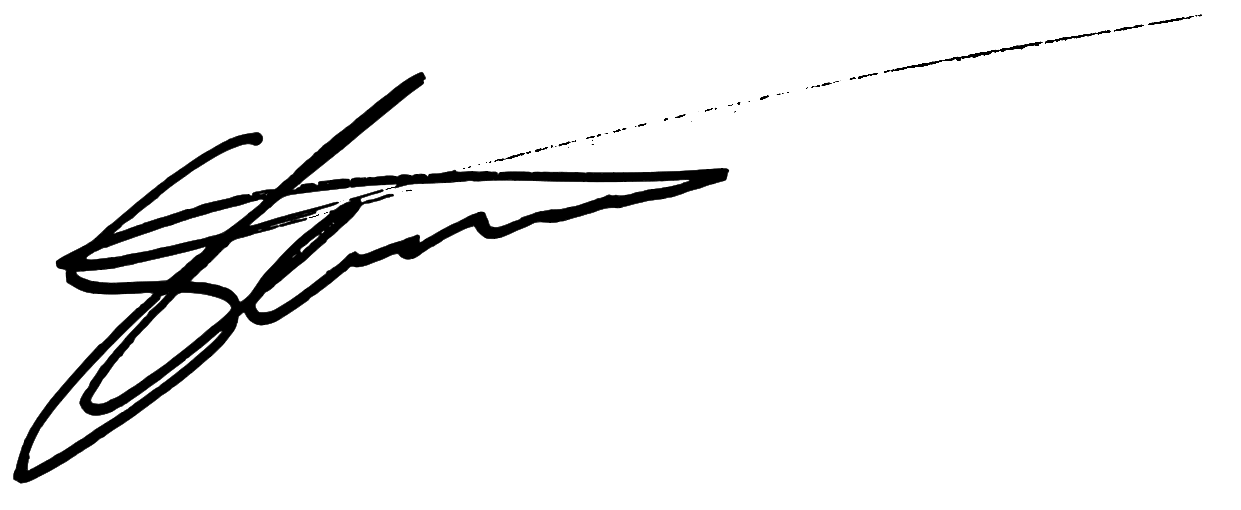
\includegraphics[width=0.5\textwidth]{Signature}\\
		\makebox[0.3\textwidth][r]{\titlerule[0.2ex]}
		
		\makebox[0.3\textwidth][r]{\fontfamily{ppl}\selectfont\textsc{Stephen Blowers}}
		
		\makebox[0.3\textwidth][r]{\fontfamily{ppl}\selectfont\textsc{Edinburgh, March 2018}}
	\end{flushright} 
	
	\fancyhead{}
	\fancyfoot[CO]{\fontfamily{ppl}\thepage}
	\fancyfoot[CE]{\fontfamily{ppl}\thepage}
	
	\newpage
	\thispagestyle{empty}	
	
	\chapter*{{\Huge L}ay {\Huge S}ummary}
	\addcontentsline{toc}{chapter}{Lay Summary}
	It has been demonstrated within the medical community that reducing the temperature of brain tissue after the event of trauma, such as a stroke or an impact to the head, provides protective benefits. An effective method to achieve this is to cool the entire body, however, this can lead to further complications such as the spread of infection in other organs. Alternatively, to avoid such developments, the brain temperature could be lowered independently to the rest of the body by cooling the surface of the head. Unfortunately, directly determining the effectiveness of this type of intervention is difficult due to the invasiveness of measuring temperatures in the brain. Instead, researchers have to rely on mathematical models and simulations to assess the outcomes of such procedures.
	
	It is believed that the current models and methods are oversimplified as they rely on Pennes Bioheat Equation, which omits any convective heat transfer caused by blood flowing through vessels and capillaries. In this thesis, an alternative method is proposed that includes blood flow in both the aforementioned vessels and capillaries to deliver a more physically representative simulation of heat transfer within the brain. This is then used to investigate how much of an effect cooling the head has on brain temperature.
	
	\newpage
	\thispagestyle{empty}
	
	\chapter*{{\Huge A}bstract}
	\addcontentsline{toc}{chapter}{Abstract}
	
	Hypothermia has been shown to provide protective benefits to the brain after head trauma. Current treatment methods employ full body hypothermia which can lead to further associated complications, such as a compromised immune system. Alternatively, cooling the brain individually can provide the same benefits whilst minimising the risks associated. Unfortunately, the feasibility of this is still uncertain due to the invasiveness of measuring cerebral temperatures directly and the unavailability of brain temperature maps.
	
	Mathematical modelling provides an important alternative avenue for predicting the outcome of hypothermic procedures, such as scalp cooling. However, these tend to rely on Pennes Bioheat Equation which simplifies the blood flow within the system as a single perfusion term. This removes any directional thermal advection which could play an important part in biological heat transfer. In this thesis, an alternative method is developed, tested, and proposed where the full cerebral circulatory system is modelled using vascular channels embedded in a porous tissue simulating the blood vessels and capillaries, respectively. This is dubbed the vascular porous (VaPor) method.
	
	This dissertation tests and discusses the feasibility of inducing hypothermia by cooling the scalp using the VaPor model. Initially, the blood vessels were modelled in 3D to fully capture the effects of flow, however, this was deemed computationally inefficient and difficult to manipulate so was subsequently replaced with a system of 1-Dimensional line segments. Temperatures produced from this method conform to expected ranges of values and agree with available data from studies in rat brains. It was observed that core brain temperatures can be impacted by scalp cooling but only with a large number of generated vessels. This is due to the tortuous nature of the vasculature which is not captured by the porous media alone. Various input parameters are also tested to ensure the validity of results from this model.
	
	One tested parameter that did not agree with \textit{in-vivo} results was the measurement of tissue perfusion which appeared to be grossly exaggerated by the VaPor model, although conservation of mass was conserved at each stage. This was investigated further by simulating tracer transport in the cerebral domain in the same manner that \textit{in-vivo} measurements use. While \textit{in-vivo} measurements and the predictions by tracer transport produce perfusion values of the same order of magnitude, a full quantitative match cannot be expected because of the differences in the measurement techniques used. Various approximations that can be imposed to resolve this are discussed.
	
	The versatility of the VaPor model was explored by simulating a variety of applications relevant to cerebral cooling. The inclusion of counter-current flow within the porous domain showed similar results to trials performed with dense vascular trees. Trials on the scale of a neonatal brain showed that hypothermia could be achieved from scalp cooling alone contrary to previous models. The transient response of scalp cooling was explored as well as the thermal response after simulating an ischemic stroke. All results demonstrated that, due to the inclusion of directional flow, scalp cooling has a larger impact on cerebral temperatures than seen with previous bioheat models. 
	
	
	\chapter*{{\Huge A}cknowledgements}
	\addcontentsline{toc}{chapter}{Acknowledgements}
	
	\begin{flushright}
		\parbox{0.7\textwidth}{\flushright\textit{``Do not pray for an easy thesis}$^{*}$\textit{, pray for the strength to endure a difficult one'' \qquad\qquad\qquad}}
		
		-- Bruce Lee
		
		\parbox{\textwidth}{\flushright\scriptsize{$^{*}$I believe, in his original phrasing, `life' was used. However, at this stage, I do not see the difference.}}
	\end{flushright}
	
	\bigskip
	\bigskip
	\medskip
	
	Firstly, I would like to thank my supervisors, Profs.\ Prashant Valluri and Ian Marshall, along with Drs.\  Bridget Harris, Peter Andrews, and Michael Thrippleton for there insight and support provided throughout this project. Their feedback and advice has been invaluable and it has been a pleasure working with them all.
	
	Additionally, I would like to extend thanks to colleagues working in the Sanderson Building. Patrick, Pedro, Esm\'e, and Nick to name just a few. James Young in particular, for giving me an outlet to vent at length about hunting nefarious bugs and `features' lurking within my jungle of code scripts.
	
	I would also like to extend my gratitude to my family, not only for supporting me over the last few years, but for their generosity and guidance that allowed me to get where I am today. I am also eternally grateful for the numerous hours of scouring this text that my father endured, weeding out the careless typos and errors that I ashamedly put in.
	
	Furthermore, I feel an acknowledgement must also go out to the Edinburgh University catering team for consistently providing me with the fuel to persevere in the form of endless gallons of coffee and an inordinate number of pastries. So frequent were my trips to the caf\'e that I believe the line between man and muffin has forever been irrevocably blurred.
	
	Suffice it to say that my greatest gratitude has to be given to Helen for putting up with the roller-coaster of emotions that the last four years has been. Many dark times, when my nerve faltered and my outlook was bleak, were brightened by your radiant smile and reassuring embrace. Understandably, this work would not have been completed without the loving care (and fantastic food!) that you provided. So, I hereby dedicate this work to you. Here's to a bright and exciting future together!
	
	\newpage
	\thispagestyle{empty}
	
	\tableofcontents

%	\cleardoublepage
%	\listoffigures%
%	\addcontentsline{toc}{chapter}{List of Figures}
%	
%	\cleardoublepage
%	\listoftables
%	\addcontentsline{toc}{chapter}{List of Tables}
\newpage
\thispagestyle{empty}

\chapter*{{\Huge L}ist of {\Huge F}igures and {\Huge T}ables}
\addcontentsline{toc}{chapter}{List of Figures and Tables}
	\begingroup
	\makebox[0.5\textwidth][l]{\sffamily\selectfont\bfseries\large\MakeUppercase{{\Large F}igures}}
	
	\makeatletter
	\@starttoc{lof}
	\makeatother
	\let\clearpage\relax
	
	\makebox[0.5\textwidth][l]{\sffamily\selectfont\bfseries\large\MakeUppercase{{\Large T}ables}}

	\makeatletter
	\@starttoc{lot}
	\makeatother
	
	\endgroup

\newpage
\thispagestyle{empty}
	\chapter*{{\Huge N}omenclature}
	\addcontentsline{toc}{chapter}{Nomenclature}
	\renewcommand{\arraystretch}{1.4}
	
	{\fontfamily{ppl}\selectfont\textsc{Latin Letters}
	\vspace*{-\baselineskip}
	\begin{center}
	\begin{longtable}[H]{L{0.1\textwidth} L{0.50\textwidth} R{0.15\textwidth}}

		$A$ & Interfacial area between voxels & $m^2$ \\
		$A_{surf}$ & Surface area of a vessel segment & $m^2$ \\
		$A_{Xsec}$ & Average cross sectional area of a vessel segment & $m^2$ \\
		$\mathbf{A}$ & Matrix of coefficients used in linear solver & -- \\
		$\mathbf{B}$ & Vector of constants used in linear solver & -- \\
		$c$ & Specific heat capacity of tissue & $J/kg/^{o}C$ \\
		$c_{b}$ & Specific heat capacity of blood & $J/kg/^{o}C$ \\
		$C$ & Concentration of tracer in blood flow & $kg/m^3$ \\
		$C_{0}$ & Initial concentration entering element & $kg/m^3$ \\
		$C_{a}$ & Arterial inlet function describing the concentration profile injected into the inlet nodes & $kg/m^3$ \\
		$C_{R}$ & Blood flow reversal factor for voxels  & --\\
		$D$ & Diameter of blood vessel segment & $m$ \\
		$D_{c}$ & Diameter of capillaries & $m$ \\
		$\mathcal{D}$ & Diffusion coefficient & $m^2/s$ \\
		$f$ & Arbitrary function used to describe convolution operation & -- \\
		$\dot{F}$ & Mass flowrate of blood & $kg/s$ \\
		$\dot{F}_{inlet}$ & Mass flowrate of blood at an inlet node & $kg/s$ \\
		$\overline{F}$ & Total mass flowrate of blood entering the brain & $kg/s$ \\
		$g$ & Arbitrary function used to describe convolution operation & -- \\
		$G$ & Conductance of blood flow through species &  $m{\cdot}s$\\
		$h_{bt}$ & Surface heat transfer coefficient for domain interface between tissue and blood phases in porous media & $W/m^2/^{o}C$ \\
		$h_{out}$ & Surface heat transfer coefficient for scalp & $W/m^2/^{o}C$ \\
		$I$ & Ideal concentration impulse function where all tracer is injected into element at $t=0$ & $kg/m^3$\\
		$I_{0}$ & Initial concentration injected into element at $t=0$ for ideal concentration impulse function & $kg/m^3$\\
		$\mathcal{I}$ & Modified Bessel function of the first kind & --\\
		$K$ & Thermal conductivity of tissue & $W/m/^{o}C$ \\
		$K_{b}$ & Thermal conductivity of blood & $W/m/^{o}C$ \\
		$K_{z}$ & Thermal conductivity of hemispherical tissue region, $z$ & $W/m/^{o}C$ \\
		$l$ & Length between 3-Dimensional voxels & $m$ \\
		$L$ & Length of vessel segments (distance between connected vessel nodes) & $m$ \\
		$m$ & Number of voxels intersected by a particular vessel segment & -- \\
		$m'$ & Number of vessel segments that intersect a particular voxel & -- \\
		$\dot{M}_{x\rightarrow y}$ & Inter-domain blood flow mass transfer (from domain $x$ to domain $y$) & $kg/s$ \\
		$n$ & Number of connections for a node, temporary node, or voxel & -- \\
		$N$ & Physical amount of tracer in blood flow & $kg$ \\
		$\mathcal{N}$ & Directional vector pointing towards adjacent element (voxel or node) & -- \\
		$\mathcal{O}$ & Order of magnitude of error from discretisation & - \\
		$P$ & Pressure & $N/m^2$ \\
		$Q_{gen}$ & Local metabolic heat generation of tissue & $W/m^3$ \\
		$Q_{gen}$ & Overall average metabolic heat generation of tissue & $W/m^3$ \\
		$Q_{C}$ & Energy transfer through conduction between elements (voxels or nodes) & $W$ \\
		$Q_{G}$ & Energy transfer from metabolic heat generation & $W$ \\
		$Q_{I}$ & Energy transfer from inter-domain conduction & $W$ \\
		$Q_{M}$ & Energy transfer from inter-domain convection from blood transfer & $W$ \\
		$Q_{Pen}$ & Energy transfer from perfusion term & $W$ \\
		$Q_{V}$ & Energy transfer from convection between elements (voxels or nodes) & $W$ \\
		$Q_{X}$ & Type of energy transfer within the VaPor model & $W$ \\  
		$r$ & Local radius length of brain & $m$ \\
		$r_{z1}$ & Lower boundary for specified hemispherical tissue region, $z$ & $m$ \\
		$r_{z2}$ & Upper boundary for specified hemispherical tissue region, $z$ & $m$ \\
		$R$ & Total radius length of brain & $m$ \\
		$\mathcal{R}$ & Normalised residual function of tracer passing through an element & -- \\
		$t$ & Time & $s$ \\
		$\overline{t}_{r}$ & Average transit time for flow through an element (voxel or node) & $s$ \\
		$\Delta t$ & Timestep & $s$ \\
		$T$ & Temperature of tissue & $^{o}C$ \\
		$T_{a}$ & Temperature of arterial blood from the body core & $^{o}C$ \\
		$T_{b}$ & Temperature of blood & $^{o}C$ \\
		$T_{out}$ & Temperature of outside environment & $^{o}C$ \\
		$T_{m}$ & Temperature rise due to metabolic heat generation & $^{o}C$ \\
		$T_{scalp}$ & Temperature of the scalp surface & $^{o}C$ \\
		$u$ & Arbitrary time variable used to describe convolution operation & $s$ \\
		$U$ & Superficial 
		velocity of blood & $m/s$ \\
		$U'$ & True 
		velocity of blood & $m/s$ \\
		$U_{r}$ & Radial superficial velocity of blood & $m/s$ \\
		$U_{R1}$ & Forward superficial velocity for voxels when using flow reversal factor & $m/s$ \\
		$U_{R2}$ & Backward superficial velocity for voxels when using flow reversal factor & $m/s$ \\
		$V$ & Volume of element (voxel or vessel segment) & $m^3$\\
		$\Delta x$ & Length step size & $m$ \\
		$\mathbf{x}$ & Vector of temperature variables used in linear solver & -- \\
		$z$ & Region of hemispherical tissue material bounded by $r_{z1}$ \& $r_{z2}$ & -- \\
		
	\end{longtable}
	\end{center}
	\pagebreak
	{\fontfamily{ppl}\selectfont\textsc{Greek Letters}
		\vspace*{-\baselineskip}
		\begin{center}
		\begin{longtable}[H]{L{0.1\textwidth} L{0.50\textwidth} R{0.15\textwidth}}
			
		$\alpha_{bt}$ & Specific surface area for domain interface between tissue and blood phases in porous media & $m^2/m^3$ \\ 
		$\beta_{x\leftrightarrow y}$ & Inter-domain heat transfer coefficient (between domain $x$ and domain $y$) & $W/^{o}C$ \\
		$\delta$ & Characteristic shielding length due to blood perfusion & $m$ \\
		$\epsilon$ & Volume fraction of domain in porous media & -- \\
		$\overline{\epsilon}$ & Average volume fraction of domain from neighbouring voxels & -- \\
		$\epsilon_{b}$ & Volume fraction of blood in porous media & -- \\
		$\kappa$ & Permeability of porous media & $m^2$ \\
		$\mu_{b}$ & Viscosity of blood & $Pa{\cdot}s$ \\
		$\rho$ & Density of tissue & $kg/m^3$ \\
		$\rho_{b}$ & Density of blood & $kg/m^3$ \\
		$\tau$ & Tortuosity of blood vessels & -- \\
		$\omega$ & Local perfusion rate of blood & $m^3/kg/s$ ($ml/100g/min$) \\
		$\overline{\omega}$ & Overall average perfusion rate of blood & $m^3/kg/s$ ($ml/100g/min$) \\
		$\Omega$ & Overall conductive thermal resistance for various head materials & $^{o}C/W$ \\
		$\Omega_{z}$ & Individual conductive thermal resistance for tissue region, $z$ & $^{o}C/W$ 
		
		\end{longtable}
		\end{center}
\vspace*{-\baselineskip}
	{\fontfamily{ppl}\selectfont\textsc{Superscripts}
		\vspace*{-\baselineskip}
		\begin{center}	
			\begin{longtable}[H]{L{0.1\textwidth} L{0.50\textwidth} R{0.15\textwidth}}
				$n$ & Denotes current timestep & -- \\
				$n+1$ & Denotes subsequent timestep & -- \\
			\end{longtable}
		\end{center}	
	\vspace*{-\baselineskip}
	{\fontfamily{ppl}\selectfont\textsc{Domain Subscripts}
		\vspace*{-\baselineskip}
	\begin{center}	
	\begin{longtable}[H]{L{0.1\textwidth} L{0.50\textwidth} R{0.15\textwidth}}
			
		$1$ & Blood within the arterial vessels & -- \\
		$2$ & Brain tissue (solid phase of porous media) & -- \\
		$3$ & Blood within capillaries (fluid phase of porous media) & -- \\
		$3a$ & Distributing blood within capillaries in counter-current model & -- \\
		$3b$ & Draining blood within capillaries in counter-current model & -- \\
		$4$ & Blood within the venous vessels & -- \\
		$adj$ & Denotes an adjacent voxel & -- \\
		$i,j,k$ & Denotes the location of a voxel in 3-Dimensional space & -- \\
		$b1$ & Distributing blood within the blood phase in counter-current hemispherical model & -- \\
		$b2$ & Draining blood within the blood phase in counter-current hemispherical model & -- \\
		$v$ & Denotes the a node within a vascular tree dataset & -- \\
		$v,adj$ & Denotes an adjacent node connected within a vasculature tree dataset & -- \\
					
	\end{longtable}
	\end{center}
	\vspace*{-\baselineskip}
		{\fontfamily{ppl}\selectfont\textsc{Dimensionless Parameters}
			\vspace*{-\baselineskip}
			\begin{center}	
				\begin{longtable}[H]{L{0.1\textwidth} L{0.30\textwidth} R{0.35\textwidth}}
					
					\Graetz & Graetz Number & $\Graetz = \frac{\rho_{b}c_{b}UD^{2}}{K_{b}L}$ \\	
					\Nuss & Nusselt Number & $\Nuss = \frac{hD}{2K_{b}}$ \\
					\Reynolds & Reynolds Number & $\Reynolds = \frac{\rho_{b}UD_{v}}{\mu_{b}}$ \\
					
				\end{longtable}
			\end{center}
			\vspace*{-\baselineskip}
		{\fontfamily{ppl}\selectfont\textsc{Acronyms}
			\vspace*{-\baselineskip}
			\begin{center}	
				\begin{longtable}[H]{L{0.1\textwidth} L{0.50\textwidth} R{0.15\textwidth}}
					AIF & Arterial Inlet Function & --\\
					CAD & Computer Aided Design & --\\
					CSF & Cerebral Spinal Fluid & --\\
					DiVa & Discrete Vasculature & --\\
					MRI & Magnetic Resonance Imaging & --\\
					MRS & Magnetic Resonance Spectroscopy & --\\
					SBC & Selective Brain Cooling & --\\
					SIMPLE & Semi-Implicit Method for Pressure Linked Equations & --\\
					STL & STereoLithography (type of file format) & --\\
					RRT & Rapidly-exploring Random Tree & -- \\
					TSE & Temperature Shielding Effect & -- \\
					TVD & Total Variance Diminishing & -- \\
					VaPor & Vascular Porous & --\\
					
				\end{longtable}
			\end{center}
	
	\renewcommand{\arraystretch}{1.2}
	
	\mainmatter	
	
	\RegularTitle
	\setcounter{chapter}{0}
	\chapter[Introduction]{{\Huge I}ntroduction}
	\fancyhead[LE]{\makebox[1cm][r]{\fontfamily{ppl}\thepage\enskip}$\mid$\enskip\makebox[1cm][l]{\fontfamily{ppl}\scriptsize\MakeUppercase{{\small I}ntroduction}}}
	\fancyfoot{}
	\thispagestyle{empty}
	
	\section[Background]{{\Large B}ackground}
	\fancyhead[RO]{\makebox[1cm][r]{\fontfamily{ppl}\small\thesection{ -- }\scriptsize\MakeUppercase{{\small B}ackground}}\enskip$\mid$\makebox[1cm][l]{\enskip\fontfamily{ppl}\thepage}}
	
	The human brain collectively stores a person's memories and personality, and therefore can be said to effectively define who somebody is. This makes it one of the most precious organs in the human body and should be protected at all costs. Fortunately, the body is engineered to defend its vital organs. The brain is surrounded by a layer of dense bone, the skull, and is cushioned by cerebral spinal fluid underneath. An arterial structure, the circle of Willis, provides a level of circulatory redundancy so that if one feeding artery becomes obstructed, the downstream tissue does not become ischemic (starved of oxygen). These are only a couple of the natural defence mechanisms that help to keep the brain protected in day-to-day life.
	
	That being said, there are still many ways brain injury can occur. Rapid sudden motion of the head, possibly caused by impact, can cause the brain to collide with the skull, causing a concussion. An example of such an injury is displayed in Figure~\ref{fig:1HeadImpactDiagram}. Associated swelling of the tissue can cause further damage as this prevents proper perfusion of blood through the tissue. Alternatively, occlusion of blood vessels (beyond the circle of Willis), such as in a stroke, or impairment of the full circulatory system in, for example, a heart attack, can cause regions of tissue to become ischemic (i.e.\ not receiving the correct level of oxygen and nutrients to sustain cellular metabolism). These injuries are not uncommon. Around 350,000 cases of acquired brain injury occurred in the UK alone between April 2013 and May 2014 \cite{headway2014statistics}. Head injuries accounted for $46.5\%$ of these while strokes accounted for $37.4\%$. Recently, there has been a drive for awareness for head injuries sustained in contact sports as it is thought that they are the source of mental disorders later on in life. Such injuries can appear minor initially, but develop into much more serious conditions.
	
	\begin{figure}[h]
		\centering
		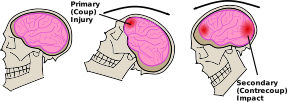
\includegraphics[width=\textwidth]{BrainConcussion}
		\caption[Example of whiplash injury]{Example of a brain injury caused by whiplash motion of the head. This can occur in situations where rapid impact is applied to the body such as in an automobile collision or receiving a tackle in a contact sport. Initially the head lurches backwards and the brain collides with the front of the skull causing the primary, or coup, injury. As the head returns sharply to its original position, a secondary, or contrecoup, injury occurs on the opposite side of the brain.}
		\label{fig:1HeadImpactDiagram}
	\end{figure}
	
	Outcomes of brain injury differ between patients and can present a wide variety of symptoms. Depending on the affected region, behavioural and emotional changes in ones personality can occur. Cognitive and physical functions such as speech or hand-eye coordination can become impaired. Some of these lost skills can be relearned by the patient but this process can take weeks, months or even years. Others are permanent.
	
	As the injury has already occurred on arrival to hospital, clinical intervention is directed towards minimising the risk of further damage generated from the biological responses to the initial injury. One method that has been shown to increase recovery is inducing hypothermia. This involves reducing the temperature of the tissue to below normal conditions which is generally considered to be $37^{o}C$ (but can fluctuate by ${\approx}0.5^{o}C$). Numerous animal and human studies have shown the benefit of induced hypothermia.
	
	As these injuries tend to warrant emergency treatment, the study of effects and experimentation of intervention methods become secondary to the overall outcome of the patient. Therefore, data is scarce and the opportunity to investigate or experiment is very limited. This is why exploration into hypothermic treatment methods tend to use predictive modelling to assess their potential benefits prior to clinical trials. Accuracy of these models is therefore crucial for determining the effectiveness of the methods in question. 
	
	\section[Objectives and Specific Aims]{{\Large O}bjectives and {\Large S}pecific {\Large A}ims}
	\fancyhead[RO]{\makebox[1cm][r]{\fontfamily{ppl}\small\thesection{ -- }\scriptsize\MakeUppercase{{\small O}bjectives and {\small S}pecific {\small A}ims}}\enskip$\mid$\makebox[1cm][l]{\enskip\fontfamily{ppl}\thepage}}
	
	It is considered that the current models used for modelling cerebral temperatures are too simplistic to correctly assess treatment methods. The majority of trials rely on the Pennes Bioheat Equation \cite{pennes1948analysis} which reduces all heat transfer associated with blood flow to a single perfusion source/sink term. While this simplification gives the model accessibility, the lack of any directional flow and advective effects of blood flow raises the question of its accuracy. Some models address this by including flow in major blood vessels but they revert back to this perfusion term at the capillary level. No current study includes the thermodynamic effects of directional flow in both large arteries and small capillaries combined.
	
	The objective of this work is two-fold. Firstly, it aims to produce a method for modelling bioheat transfer that includes the full directionality of blood flow by incorporating both macro-level flow using detailed blood vasculature and micro-level flow with porous media approximating the capillaries. Secondly, it aims to explore the feasibility and effectiveness of reducing core brain temperature non-invasively using the scalp cooling. Work towards these two objectives was performed in parallel, with the specific physical aspects required to model the brain influencing the methods used in the bioheat model. 
	
	\section[Overview of Dissertation]{{\Large O}verview of {\Large D}issertation}
	\fancyhead[RO]{\makebox[1cm][r]{\fontfamily{ppl}\small\thesection{ -- }\scriptsize\MakeUppercase{{\small O}verview of {\small D}issertation}}\enskip$\mid$\makebox[1cm][l]{\enskip\fontfamily{ppl}\thepage}}
	
	The remainder of this work is outlined as follows: Chapter~\ref{Sec:1Chapter1} explores the literature relevant to the treatment of head trauma using hypothermia along with the various methods of modelling bioheat temperatures. As many of these models omit the directionality of blood flow, Chapter~\ref{Sec:2Chapter2} introduces this concept to the subject of cerebral cooling. Initially simple 1-Dimensional models are used, as previously performed in literature, which are then expanded to full 3-Dimensional model with detailed vasculature. Due to limitations found in in applying this method, which would require infeasible levels of computational resource to overcome, the 3-Dimensional vasculature was replaced with 1-Dimensional line segments. This also allowed for more flexibility with the model. As this involves the embedding of 1-D vasculature in porous media, this method was dubbed the Vascular Porous (VaPor) model. The methods used for the VaPor model are detailed in Chapter~\ref{Sec:3Chapter3} along with results of temperature changes within the brain from instigating scalp cooling. Chapter~\ref{Sec:4Chapter4} explores the difference between blood perfusion measured within the VaPor model and those found in literature. This is mainly due to measurement techniques of flow which are explored by various means. Further exploration into aspects of the VaPor model along with some preliminary applications to clinically relevant situations are shown in Chapter~\ref{Sec:5Chapter5}. Lastly, the conclusion and direction of future work are given in Chapter~\ref{Sec:6Chapter6}.
	
	The VaPor code outlined and used in Chapter~\ref{Sec:3Chapter3} has been made open-source at [\texttt{https://github.com/sblowers/VaPor}].
	
	\newpage
	\thispagestyle{empty}
	\setcounter{chapter}{1}
	\chapter[Review of the Relevant Literature]{{\Huge R}eview of the {\Huge R}elevant {\Huge L}iterature}
	\fancyhead[LE]{\makebox[1cm][r]{\fontfamily{ppl}\thepage\enskip}$\mid$\enskip\makebox[1cm][l]{\fontfamily{ppl}\scriptsize\MakeUppercase{{\small R}eview of {\small R}elevant {\small L}iterature}}}
	\thispagestyle{empty}
	\label{Sec:1Chapter1}
	
	\section[Therapeutic Hypothermia]{{\Large T}herapeutic {\Large H}ypothermia}
	\fancyhead[RO]{\makebox[1cm][r]{\fontfamily{ppl}\small\thesection{ -- }\scriptsize\MakeUppercase{{\small T}herapeutic {\small H}ypothermia}}\enskip$\mid$\makebox[1cm][l]{\enskip\fontfamily{ppl}\thepage}}
	
	\subsection{History}
	
	Although not a novel concept, the use of induced hypothermia as an intervention method has only gained momentum in recent decades. It been recorded as early as 3500 {B.C.} in the Edwin Smith Papyrus, an ancient Egyptian text on medicine and surgery \cite{wang2006cold}. Throughout history, physicians have experimented with the application of cold to the human body to treat a wide variety of clinical disorders and in some cases used as a rudimentary anaesthetic \cite{karnatovskaia2014therapeutic}. Other instances have shown that subjecting the body to cooler temperatures can cause people to survive conditions which would otherwise prove fatal. There have been cases whereby following submersion in cold water (${<}10^{o}C$) for over 15 minutes (and in a single case over an hour), full recoveries were made with intact neurological function \cite{bolte1988use} (and sources therein). In 1650, it was recorded that on a particularly cold December day (precise temperature not given), a woman was hanged, but upon starting a dissection of the body the following day, she was discovered to be alive and proceeded to make a full recovery \cite{breathnach2009intensive}. In spite of the neuro-protective aspects of hypothermia being observed throughout history, the technique only entered modern day medicine in the latter half of the 20$^{\text{th}}$ century.
	
	Throughout the 1900s, interest in hypothermic treatment fluctuated. Although increased survival rates and neurological benefits were cited, due to the severity of the induced hypothermia, negative side effects overshadowed the positive results \cite{karnatovskaia2014therapeutic}. However, towards the late 1980s, a resurgence of interest occurred when it was shown that similar protective benefits to neurological outcome could be induced with milder hypothermia \cite{gilston1985another}. 
	
	Many studies performed in animals showed promise for hypothermia. Advantageous outcomes were demonstrated in rats with induced ischemic damage \cite{busto1987small}\cite{thoresen1996posthypoxic}. Sirimanne~\textit{et al.\ }found that to the most protection was obtained with 72 hours of induced hypothermia after the initial injury \cite{sirimanne1996effect}. This agrees with trials performed using canines which showed the best results were achieved with a treatment time of 48--96 hours for a similar ischemic injury \cite{leonov1990moderate}. Reducing the body temperature in neonatal piglets for a period of 12 hours reduced the severity of induced ischemic injuries \cite{thoresen1995mild}\cite{amess1997mild}. Trials in humans also showed positive long term outcomes for patients presenting with severe head trauma \cite{marion1993use}\cite{marion1997treatment}.
	
	Current medical practice advises the use of hypothermia as a treatment method. The National Institute for Health and Care Excellence recommends that comatose patients post-cardiac arrest should have their temperatures reduced to $32^{o}C$--$34^{o}C$ for 12--24 hours (IPG386, March 2011) \cite{nice2011therapeutic}. Although, by the time this recommendation was published, 85.9\% of UK hospitals had already adopted hypothermia treatment in their post-cardiac arrest care \cite{binks2010therapeutic}. The same advice is given by the American Heart Association but recommends a wider range of target temperature, $32^{o}C$--$36^{o}C$ \cite{neumar2015part}.
	
	\subsection{Effects of Inducing Hypothermia}
	
	Meta-analysis of studies performed shows that inducing hypothermia generally has positive effects on the neurological outcome for patients presenting with cardiac arrest \cite{arrich2016hypothermia} or head trauma \cite{crossley2014systematic}. The exact reason for the protection bestowed by hypothermia is still not known and probably varies from patient to patient. However, many favourable response mechanisms have been identified and the protective benefits are most likely a combination of these various factors. It has been shown that hypothermia reduces the rate of metabolism in cerebral tissue \cite{michenfelder1991relationship}. Not only does this prevent the tissue from becoming ischemic by reducing the oxygen demand, hypothermia also suppresses the biochemical responses to cells following the onset of ischemia \cite{busto1989effect}. The cooler temperatures can also suppress the inflammatory response of tissue following trauma \cite{karnatovskaia2014therapeutic} and additionally reduce intracranial pressure which can prevent damage caused by inflamed tissue \cite{polderman2004application}. Reintroducing blood to ischemic regions can cause reperfusion injuries, however, these appear to be curtailed with applied hypothermia \cite{karnatovskaia2014therapeutic}. Additionally, during this phase, hypothermia also helps to preserve the integrity of the blood brain barrier which helps prevent the diffusion of disruptive cytotoxic elements from the blood to the brain cells \cite{polderman2009mechanisms}.
	
	
	The clinical definition of hypothermia remains somewhat ambiguous. Some claim hypothermia is a core body temperature lower than $35^{o}C$ \cite{brown2012accidental}. However, Polderman \& Herold state hypothermia is defined as a core body temperature lower than $36^{o}C$  \cite{polderman2009therapeutic}. They also stress the difference between accidental hypothermia and therapeutically induced hypothermia which can initiate difference response mechanisms from the body. Because of this ambiguity, the exact target reduction in brain temperature to incite neurological protection is unknown. However in practice, target temperature is usually $32^{o}C$--$35^{o}C$ \cite{karnatovskaia2014therapeutic}\cite{arrich2016hypothermia}. It has also been shown that the elevation of cerebral temperatures in similar scenarios worsens outcomes, therefore even small changes in core brain temperature offsetting this could be clinically relevant \cite{mariak2002intracranial}.
	
	Care should be taken as too much cooling can have a detrimental effect on patient outcome. Gupta~\textit{et al.\ }state that reducing brain temperature to below $35^{o}C$ causes impairment of cerebral oxygenation and no improvement to neurological outcomes \cite{gupta2002effect}. In results from a multi-centre trial by Clifton~\textit{et al.}, reducing the brain temperature to $33^{o}C$ showed no overall improvements to traumatic brain injured patients \cite{clifton2001lack}. However, this trial included patients that arrived in an already hypothermic conditions, which could indicate a higher degree of injury severity.
	
	To ensure hypothermic conditions are met within the brain, most clinical methods apply full body hypothermia. This can be achieved via either internal methods through injecting cold saline solution intravenously \cite{bernard2003induced} or externally through surrounding the patient with cooling blankets or applying evaporative solutions such as alcohol to the skin \cite{polderman2004application}. Assuming the core body temperature is constant throughout the body, this allows for good control for achieving the targeted temperature as it is more easily measured. 
	
	Outside of intervention in emergency cases, it is possible that therapeutic cerebral hypothermia could have other neurological applications. Bagi{\'c}~\textit{et al.\ }showed a reduced frequency of epileptic seizures in patients after they underwent regular sessions of scalp cooling \cite{bagic2008towards}. Schwid~\textit{et al.\ }showed modest self-assessed improvement in patients suffering from multiple sclerosis after regular periods of light or intensive cooling \cite{schwid2003randomized}. The same application can be used to prevent the damaging elevation of cerebral tissue temperature in the event of inflammation or fever. In rats, increasing the temperature of ischemic brain tissue led to consistently worse neurological outcomes \cite{busto1987small}.
	
	\subsection{Selective Brain Cooling (SBC)}
	
	One of the drawbacks of inducing therapeutic full-body hypothermia is that it can lead to further complications \cite{karnatovskaia2014therapeutic}. Shivering might occur as a natural response to the induced hypothermia which can counteract the imposed cooling. This can also be troublesome if the patient has a sensitive injury that could be aggravated from violent movement. Additionally, at lower temperatures, the immune system can become compromised, posing further risk to the patient's well-being \cite{soleimanpour2014main}. 
	
	A solution to this would be to induce selective brain cooling (SBC) whereby the brain is cooled independently whilst maintaining the body's core temperature at normal levels. However, the mechanisms to allow this and theoretical feasibility of application in humans have been highly contentious \cite{white2011point}\cite{nybo2011counterpoint}. SBC has been shown to occur in many animals, including mammals, due to the presence of a carotid rete (also known as a rete mirablia) \cite{jessen2001selective}. This is a dense mesh of arteries near the brain that are cooled by venous blood from facial extremities. Humans do not possess this anatomical feature and generally resort to other methods for reducing bodily temperature, such as perspiration. Other mechanisms have been suggested that could allow similar effects to occur within humans but none have been proven. 
	
	Types of mechanism include the circulation of cerebral spinal fluid (CSF), the proximity of the upper airway passage to the brain, and the emissary veins in the skull. Zenker \& Kubik argue that many arterial branches are exposed to CSF and are of the order of magnitude similar to those found in carotid retes in other animals \cite{zenker1996brain}. These could benefit from the cooling as CSF is transported through the spine and therefore exposed by the large surface area of the back. Cabanac quotes that up to 100W is removed via evaporative cooling within the upper nasal passageway  \cite{cabanac1993selective}. As the roof of the nasal cavity is in such close proximity to the cranial cavity, they argue this must have an effect on cerebral temperatures. The emissary veins connect the vessels in the scalp to the superior cerebral veins. These are valveless which allows flow to occur in either direction. Cabanac \& Brinnel showed that during hyperthermia, blood flows from the cooler scalp towards the brain, but during hypothermia little to no flow occurs \cite{cabanac1985blood}. They use this as an argument to support SBC.
	
	The arguments vary with different angles on whether this phenomena occurs naturally or whether it can even be induced artificially. As the head is located relatively close to the heart, and due to the large relative blood flow it receives, it is argued that de-coupling the temperatures of the two regions is infeasible.
	
	\subsection{Cerebral Temperature Measurement}
	
	One of the main limiting aspects for determining the possibility of SBC in humans is the lack of direct brain temperature techniques. Direct measurements of cerebral temperature are rare due to the invasiveness of the procedure. Different locations and different techniques for acquiring surrogate temperatures could lead to misappropriation of SBC \cite{maloney2001rectal}. Proponents for SBC use the measurement of tympanic (eardrum) temperature as a good indication of cerebral temperature \cite{cabanac1979natural}. However, opponents to SBC in humans point to the fact that tympanic temperature is unreliable as it can be impacted by surface skin temperature \cite{nelson1998brain}.
	
	More recently, advances in magnetic resonance spectroscopy (MRS) has allowed temperature profiles of the human brain to be created non-invasively. Using the comparison of chemical shifts between water and N-acetylaspartate within the brain, a local estimate of tissue temperature can be produced \cite{cady1995estimation}. However, the accuracy of these methods has been questioned, and the lack of a `gold-standard' to compare results to inhibits validation of the method. Thrippleton~\textit{et al.\ }saw an average voxel-to-voxel variation of $0.54^{o}C$ in MRS imaging data of 31 healthy male volunteers  \cite{thrippleton2014reliability}. These unexpectedly large variations were attributed to possible systematic errors arising from the varying properties between grey and white matter.
	
	\subsection{Methods for Inducing SBC in Humans}
	
	There are a variety of methods available to attempt to artificially induce SBC in humans for intervention purposes. Non-invasive methods tend not to produce significant results. Andrews~\textit{et al.\ }attempted to reduce brain temperature using airflow passed through the respiratory tract in brain-injured patients but produced no statistically significant results \cite{andrews2005randomized}. Nybo~\textit{et al.\ }showed that face fanning had no effect on jugular venous blood temperature, an indication the brain temperature was unaffected \cite{nybo2002inadequate}. However, using MRS measurements, Harris~\textit{et al.\ }found in a study of five healthy adults that a convective cooling head device reduced average brain temperature by $0.45^{o}C$ while oesophageal temperatures were lowered by an average of only $0.16^{o}C$ \cite{harris2008forced}.
	
	While intra-vascular cooling has been deemed an effective method to achieve full body hypothermia, it is possible to use the carotid arteries to deliver a more local cooling. However, due to recirculation of blood, this method would eventually reduce the core body temperature as well, and therefore SBC would not be achieved. Choi~\textit{et al.\ }demonstrated introduction of isotonic saline into an internal carotid artery reduced jugular venous bulb temperature more than systemic temperature, indicating possible SBC \cite{choi2010selective}.
	
	Although it has not yet been shown to be successful, a non-invasive method for brain cooling following cerebral trauma makes intervention more accessible and therefore the beneficial effects outlined above may be introduced sooner. A cooling cap, for instance, if shown to be able to reduce core brain temperatures selectively, could be used as a first-response treatment for cases such as heart attack, stroke, or even concussions prior to the arrival of the emergency services.  
	
	\section[Modelling Bioheat Temperatures]{{\Large M}odelling {\Large B}ioheat {\Large T}emperatures}
	\fancyhead[RO]{\makebox[1cm][r]{\fontfamily{ppl}\small\thesection{ -- }\scriptsize\MakeUppercase{{\small M}odelling {\small B}ioheat {\small T}emperatures}}\enskip$\mid$\makebox[1cm][l]{\enskip\fontfamily{ppl}\thepage}}
	
	Due to the lack of cerebral temperature measurement techniques available, researchers have turned to mathematical bioheat modelling for investigating SBC in humans. The most common of these bioheat modelling methods are continuum models, whereby the tissue is simulated as a single physical entity, incorporating all features such as blood vessels and metabolic effects into a single equation. This simple approach allows good approximation of results without specialist computational knowledge. An alternative to the continuum model is the use of porous media whereby the tissue is split into its fluid and solid parts. Recently, discrete vasculature models have appeared, where the major vessels are modelled separately to the surrounding tissue in order to capture the associated heat transfer effects.
	
	\subsection{Continuum Models}
	
	Current continuum bioheat models for cerebral tissue temperatures generally adhere to the Pennes Bioheat Equation put forward by Pennes in 1948 \cite{pennes1948analysis}. Based on direct measurements in a human forearm, Pennes put forward a perfusion heat source term, $\omega$, that determines the heat provided (or removed) by the flowrate of blood to a certain region of tissue and the difference of temperature between the tissue and core. The overall bioheat equation can be written as:
	
	\begin{equation}
	\rho c\frac{\partial T}{\partial t} = K\nabla^{2}T - c_{b}\omega(T-T_{a}) + Q_{gen}
	\label{Eq:OrigPennes}
	\end{equation}
	
	Here, $\rho$ denotes density and $c$ represents specific heat capacity. The variables, $T$ and $t$, are temperature and time respectively. The value, $K$, is the conductive heat transfer coefficient, $T_{a}$ refers to the temperature of inlet arterial blood, and $Q_{gen}$ is the heat produced from metabolism. The subscript, $b$, denotes a property of blood whereas physical parameters without subscript refer to the tissue phase. 
	
	Within this model, the tissue temperature is governed by three parameters: conduction, blood perfusion, and metabolic heat generation shown on the right hand side of Equation~\ref{Eq:OrigPennes}. This means that only a handful of physical values are needed, which are relatively easy to obtain. 
	
	Due to its simplicity, Equation~\ref{Eq:OrigPennes} has been widely studied and applied to a variety of situations \cite{wissler1998pennes}. In the field of inducing hypothermia, a number of studies have been performed by approximating the brain to be hemispherical in shape and with cooling applied to the scalp, whereby the spherical form of Equation~\ref{Eq:OrigPennes} can be solved directly or through numerical methods \cite{nelson1998brain}\cite{xu1999mathematical}\cite{zhu2001theoretical}\cite{sukstanskii2004analytical}\cite{sukstanskii2007theoretical}. These all come to the same conclusion that scalp cooling is ineffective at inducing hypothermia within core regions of the brain as the temperature profile is predominantly uniform and unchanged between normothermia and applied cooling, save for a sharp decline towards the surface. The main cause for this was the high levels of perfusion present within the brain as it receives 20\% of cardiac output despite occupying only 2\% of the overall body weight. This phenomena was then dubbed the `temperature shielding effect' of blood perfusion within the brain tissue and the corresponding model was subsequently demonstrated in rat brains \cite{zhu2006body}\cite{zhu2009body}. Representative temperature profiles displaying this effect can be seen in Figure~\ref{fig:PennesTemperatureExample}.
	
	\begin{figure}[h]
		\centering
		\begin{subfigure}{0.49\textwidth}
			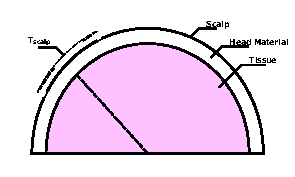
\includegraphics[width=\textwidth]{1DHemisphere/hemisphere3}
		\end{subfigure}
		\begin{subfigure}{0.49\textwidth}
			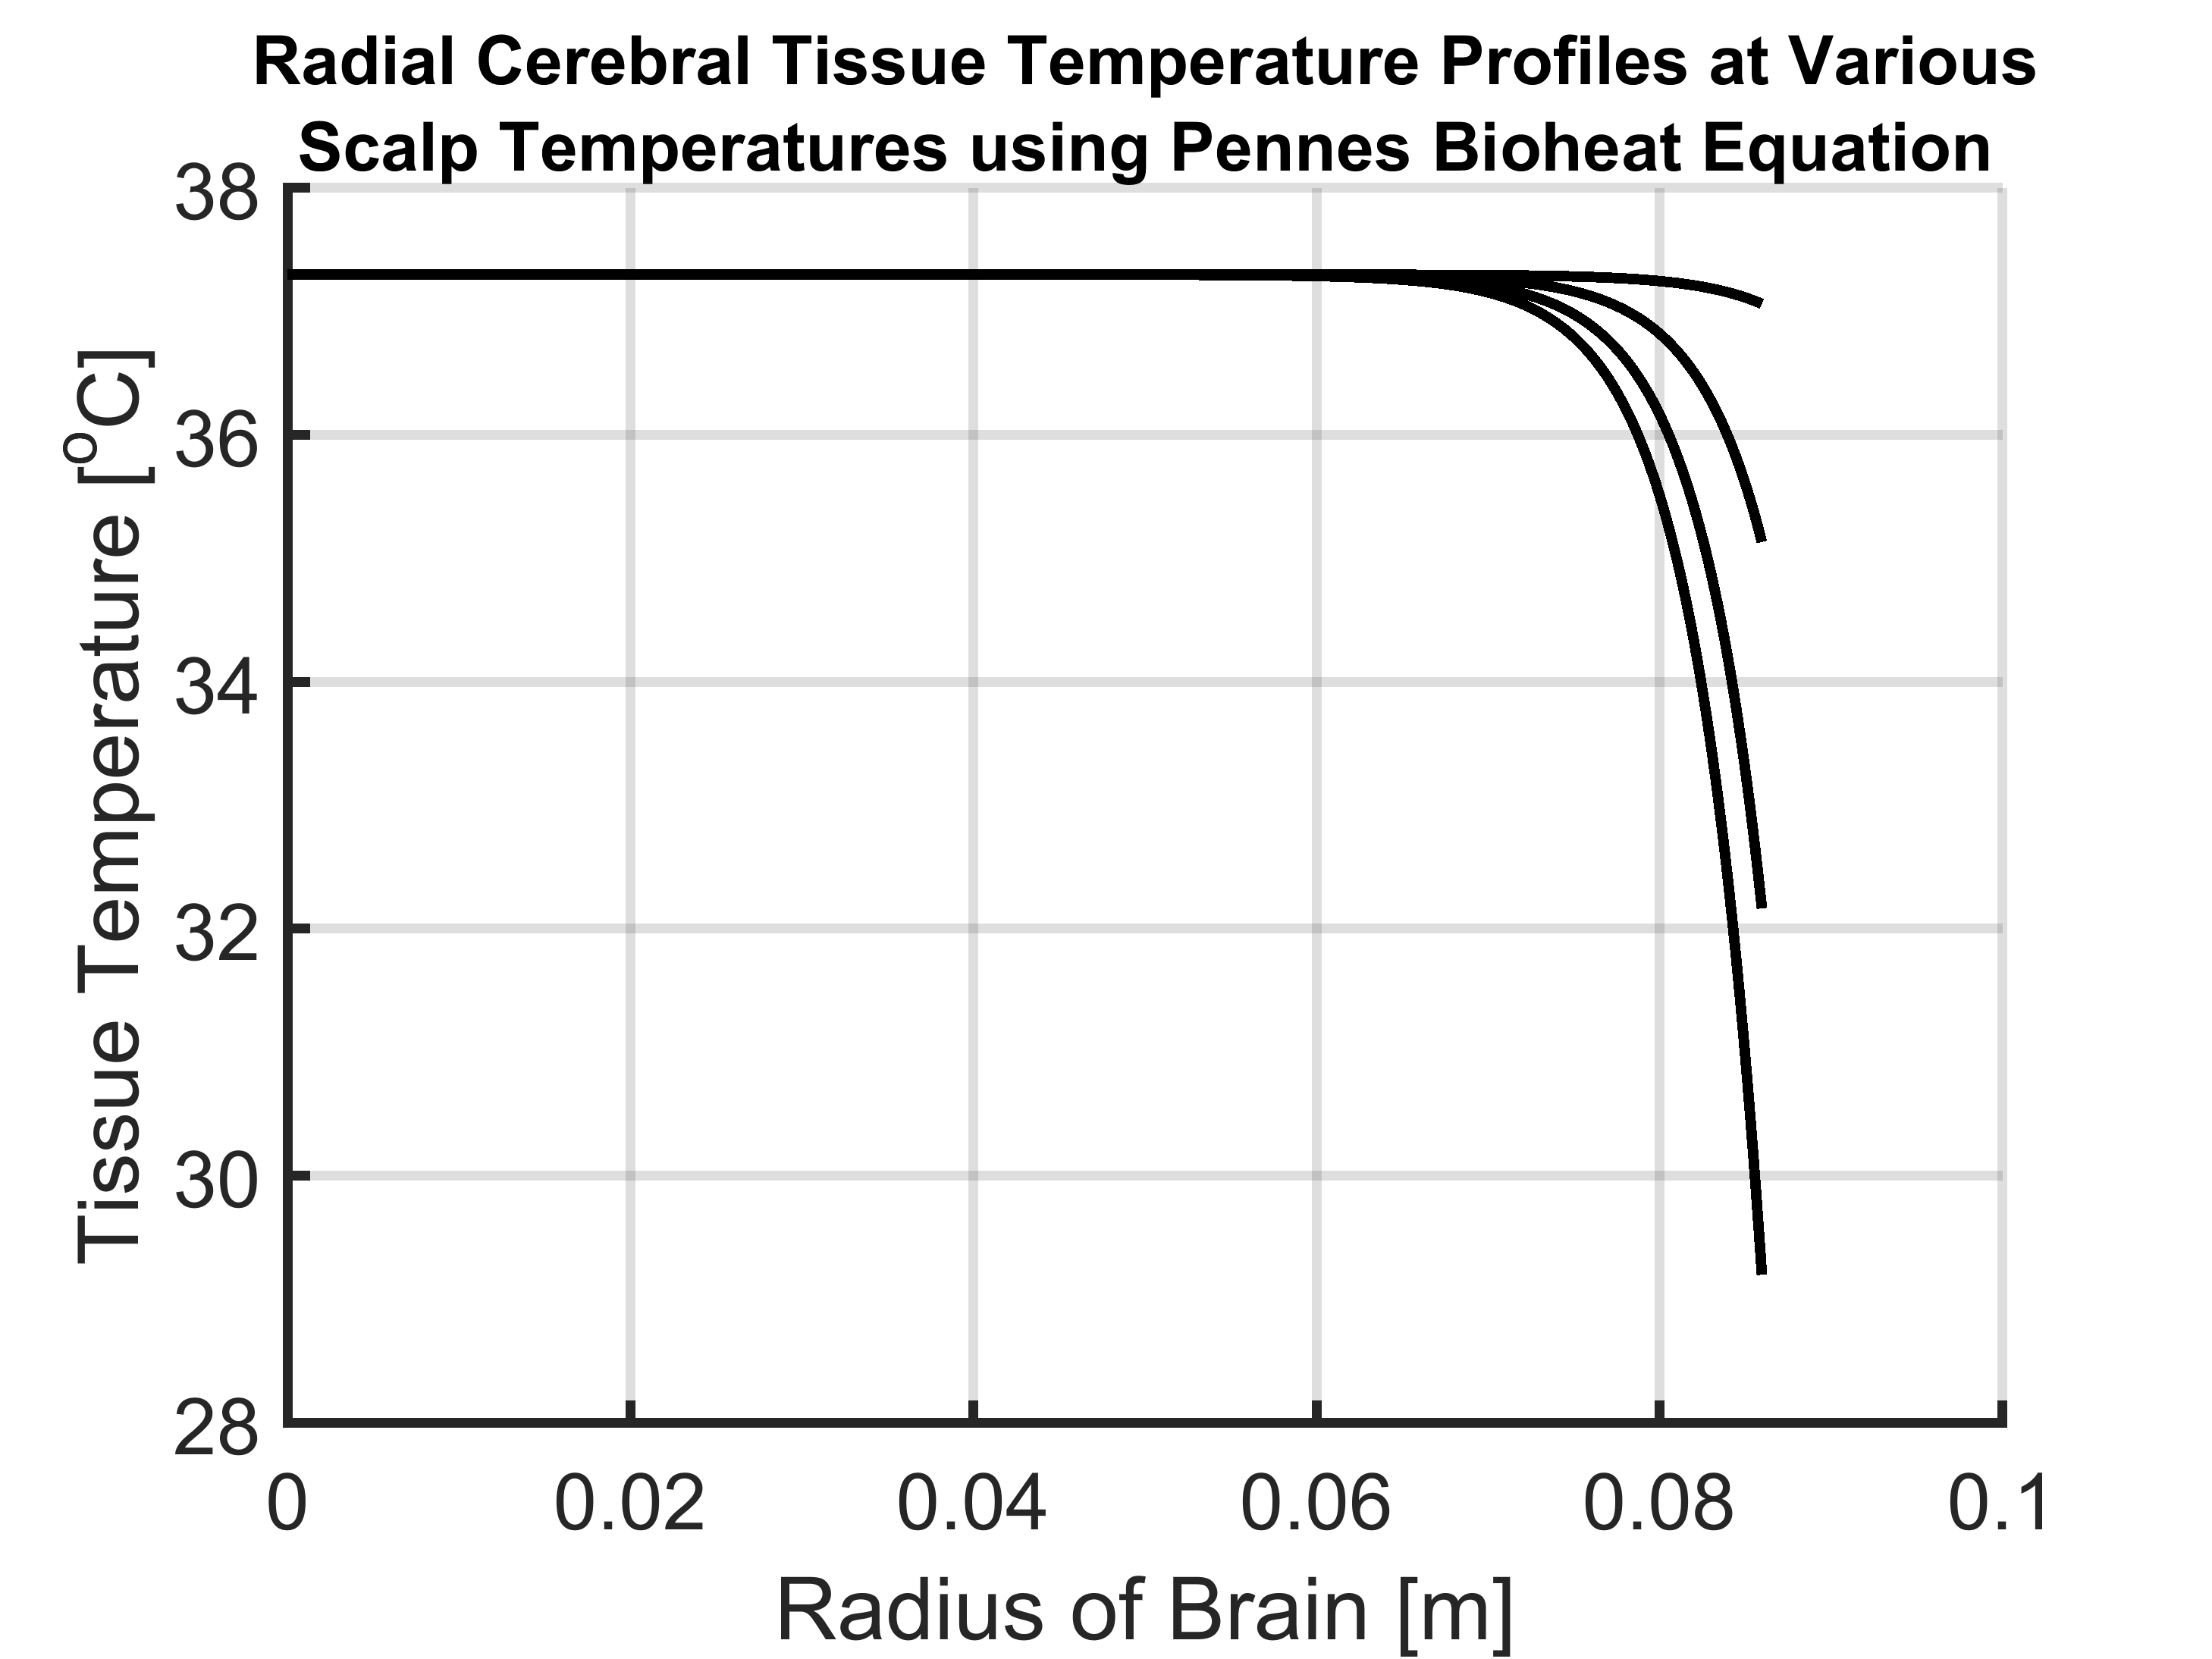
\includegraphics[width=\textwidth]{Chapter1_PennesProfiles}
		\end{subfigure}
		\caption[Typical domain and temperature profiles for cerebral bioheat models found in literature using Pennes Bioheat Equation]{Left: Typical domain for determining cerebral temperatures. The brain is approximated as a hemisphere surrounded by head material. For scalp cooling, the temperature at the scalp is set. Right: Typical radial temperature profiles generated for the domain shown on the left for different scalp temperatures. The four profiles from top to bottom are for scalp temperatures, $T_{scalp}$, of $36.5^{o}C$, $30^{o}C$, $20^{o}C$, and $10^{o}C$. Although the tissue temperatures nearer the surface are affected, temperatures beyond ${\approx}2cm$ deep into the brain are unaffected by scalp temperature. This is known as the `temperature shielding effect' of  blood flow \cite{zhu2006body}. The method for obtaining these results is explained in Section~\ref{Sec:21DHemisphere}.}
		\label{fig:PennesTemperatureExample}
	\end{figure}
	
	Alternative methods for inducing SBC have been investigated using a combination of Pennes Bioheat Equation and the directional flow of large arteries. A similar conclusion was reached when reducing inlet arterial blood temperatures through neck cooling \cite{nunneley1994limitations}\cite{zhu2000theoretical}. The relatively high levels of perfusing blood in tissue prevented the blood in the main vessels from being affected by surface cooling. However, positive theoretical results were shown if the carotid artery in question was directly cooled through invasive means \cite{wang2007targeted}. This was then validated \textit{in-vivo} with rats \cite{wang2008targeted}. Konstas~\textit{et al.\ }presented a model to explore the effects of intracarotid cooling to implement SBC \cite{konstas2007theoretical}. Although still relying on a hemispherical approximation of the brain, this domain was then segmented based on the vascular domains which receive blood from various outlets of the circle of Willis \cite{neimark2007integration}. Using this model, Neimark~\textit{et al.\ }showed a cooling cap could maintain hypothermic temperatures that were reached through intracarotid cooling \cite{neimark2008brain}. Although still relying on Pennes Bioheat Equation to solve the temperature distribution, this model had many physical parameters such as metabolism and perfusion coupled with temperature, adding some level of complexity omitted in the previous models. However, they still reached the same conclusion that scalp cooling alone was ineffectual \cite{neimark2008brain}.  
	
	Although widely used, Pennes Bioheat Equation has been subject to criticism \cite{nelson1998invited}. Wulff pointed out that the perfusion term does not take into account any directional blood flow and therefore any advective terms are omitted \cite{wulff1974energy}. He proposed a new bioheat equation that included this which was then generalised by Klinger \cite{klinger1978heat}:
	
	\begin{equation}
	\rho c\frac{\partial T}{\partial t} = K\nabla^{2}T -\rho_{b}c_{b}\nabla(UT) + Q_{gen}
	\label{Eq:OrigWulffKinger}
	\end{equation}
	
	Where $U$ is the velocity vector of blood flow, and all other variables are the same as in Equation~\ref{Eq:OrigPennes}. Although the advection term contains the physical parameters for blood, the tissue temperature is used as it is assumed that the blood and tissue temperatures rapidly reach equilibrium. Therefore, as in Equation~\ref{Eq:OrigPennes}, only a single temperature is used throughout.
	
	The addition of directionality of flow to heat transfer can dramatically affect the temperature profiles produced, most notably if the flow is directed towards or away from the cooler surface of the skin. Drawbacks to this is that the velocity profile of blood is usually not readily available and cannot be derived directly from the type of tissue present as with perfusion.
	
	Further improvements to Pennes' model looked to include the contribution of large arteries into the bioheat model as these act as strong heat sinks or sources. Chen \& Holmes developed a model that combined the advection of blood assumed to be in the larger arteries, with the perfusion term in Equation~\ref{Eq:OrigPennes} along with effective thermal conductivity associated with this perfusion \cite{chen1980microvascular}. Similarly, Weinbaum \& Jiji noted that many blood vessels operate in counter-current pairs of arteries and veins which would promote heat exchange and that this is the dominant mechanism in bioheat transfer \cite{weinbaum1985new}. 
	
	However, the last two models require additional inputs and knowledge of the inner vascular workings that are not always available or measured easily. Even the Wulff/Klinger equation requires knowledge of the velocity field of blood within the tissue. Therefore, very few applications of continuum models outside of Pennes Bioheat Equation are seen in literature due to the additional parameter requirements other than a single perfusion term for the tissue.
	
	\subsection{Porous Media}
	
	In contrast to modelling biological materials as a single entity, it is possible to subdivide them into two regions. The first includes the cells  and other structural matter of the tissue and the other contains the extra-cellular space where the blood flow occurs. This was shown in the Chen \& Holmes model \cite{chen1980microvascular}, however, by assuming the temperatures of the two regions tended to reach equilibrium quickly, they could combine their equations into a single model.
	
	Nicholson explores the mechanism of diffusion in biological porous medium in the context of mass transfer applications \cite{nicholson2001diffusion}. Nakayama \& Kuwahara were able to show that many of the continuum models could be expressed under the theory of porous media using different assumptions \cite{nakayama2008general}\cite{nakayama2011general}. Nakayama~\textit{et al.\ }proposed a three volume fraction method consisting of the tissue phase and then separate phases for the arterial and venous blood domains \cite{nakayama2010rigorous}. In this model, the heat transfer between phases was a combination of both an interfacial heat transfer term and a perfusion term as in Equation~\ref{Eq:OrigPennes}. Khaled \& Vafai also compare previous bioheat models to the theory of biological porous media \cite{khaled2003role}. The analytical solutions for these equations are then found for a variety of different physical conditions in a simple geometry \cite{mahjoob2009analytical} in the context of hyperthermia treatment. However, this model only uses a two phase system with only interfacial heat transfer.
	
	Applications of bioheat predictions using porous media include Majchrzak \& Turchan who showed that various configurations of porous media and blood flow affected the transient temperatures of a tumour undergoing hyperthermia treatment \cite{majchrzak2013numerical}. Xuan \& Roetzel simulated a three phase model in the human forearm whereby the directional flow of the arterial and venous blood to and from the extremities was counter-current \cite{xuan1997bioheat}. They also employed this model to investigate the transient response to thermal stimulus at the extremities \cite{roetzel1998transient}. These applications showed that the inclusion of directional flow, both unidirectional and counter-current had significant effects on the resultant temperature profiles.
	
	\subsection{Discrete Vascular (DiVa) Model}
	
	Implementing complex information such as vascular geometry into a continuum model is not straight-forward and can involve many assumptions of the effect of differently size vessels. Instead, it is possible to model the vessels themselves as a separate domain and calculate the interactions. Therefore, aspects such as the counter-current heat exchange need not be assumptions as the effects would be readily modelled by the geometries.
	
	The most prominent example of this is the Discrete Vascular (DiVa) model which embeds vessels as 1-Dimensional line segments into a 3-Dimensional domain \cite{kotte1996description}. Flow of blood is modelled along these segments and then transferred to the tissue domain via source and sink terms that correspond to a local perfusion term for the tissue. This is combined with convective heat transfer from direct interfacial contact of these segments with adjacent tissue. The model avoids simulating vessels smaller than $0.2mm$ in diameter \cite{kotte1999modelling} as these have been determined to be `thermally insignificant' by Chato \cite{chato1980heat}. Due to their small diameters, these vessels rapidly reach equilibrium with their surroundings and are then modelled using a perfusion term, as in Equation~\ref{Eq:OrigPennes}, but with the arterial temperature based on local surrounding arteries. This model was then validated with direct measurements from an artificially perfused bovine tongue \cite{raaymakers2000modelling}. 
	
	The model was applied to a neonatal head and results agreed with the continuum models where the core brain temperatures remained unaffected when cooled \cite{van2000numerical}. The only significant differences in temperature appeared around the large arteries and veins where blood flows were the highest. Other applications involve temperature distributions in the human eye \cite{flyckt2006modelling} and radio-frequency heating of the head \cite{van2012radiofrequency}. Both these cases also showed good qualitative agreement between the DiVa model and Pennes Bioheat Equation. 
	
	\subsection{Combining Discrete Vasculature with Porous Media}	
	
	While the DiVa model resolves the capillary bed stage of their model with a perfusion term, a combination of discrete 1-Dimensional segments inside 3-Dimensional tissue can be implemented within porous media instead. D'Angelo \& Quarteroni showed how theory for modelling water flow through a cracked porous rock bed could be applied to vascular perfused capillary bed \cite{d2008coupling}. This combined the two concepts of discrete vasculature and porous media but only simulated transport by diffusion in the porous phase. A similar approach has been performed for simulating oxygen perfusion in a capillary bed with embedded vascular structure \cite{secomb2000theoretical}\cite{secomb2004green}. Reichold~\textit{et al.\ }presented a `vascular graph' model which included both 1-Dimensional line segments in a porous 2-Dimensional area and described transport of an arbitrary scalar throughout the system \cite{reichold2009vascular}. This model was applied to drug delivery in various healthy and cancerous alveoli \cite{erbertseder2012coupled}. Recently, He \& Liu, proposed a coupled continuum-discrete bioheat model for implementing vasculature in porous tissue \cite{he2017coupled}. Many parallels can be drawn with this model and the DiVa model, such as mass transfer (and associated heat transfer) to the capillary region being condensed into a source term, and no advection from blood flow present at this level. The main difference between the two models is the resolution of interfacial heat transfer between the vessels and the adjacent tissue.
	
	Whilst there are prior examples to modelling both blood vessels and porous media, none have applied these methods to exploring hypothermia. The current work could help to expand upon this limited pool of simplified trials whereby the dominant heat transfer is dictated by the perfusion term in Pennes Bioheat Equation. 
	
	\section[Blood Flow Modelling]{{\Large B}lood {\Large F}low {\Large M}odelling}
	\fancyhead[RO]{\makebox[1cm][r]{\fontfamily{ppl}\small\thesection{ -- }\scriptsize\MakeUppercase{{\small B}lood {\small F}low {\small M}odelling}}\enskip$\mid$\makebox[1cm][l]{\enskip\fontfamily{ppl}\thepage}}
	
	\subsection{Types of Blood Flow Modelling}
	
	In order to determine the directionality of blood in the heat transfer equations, the overall flowrates have to be solved. Within the DiVa model, these are governed by the set flows at the inlets, outlets, and branch intersections of the vascular trees \cite{kotte1996description}. The advection of heat is then linearly interpolated over each branch segment. In Reichold~\textit{et al.}, the flows through the vascular tree are solved through the assumption that the hydraulic pressures in the 1-Dimensional system are analogous to voltages in an electrical circuit \cite{reichold2009vascular}. As the flowrates within blood vasculature have such low Reynold's Numbers ($\Reynolds{<}200$), they are almost certainly laminar and all the pressure drops for vessel segments can be resolved using the Hagen-Poiseuille equation. A similar method was employed in Neimark~\textit{et al.\ }to determine the distribution of blood by the circle of Willis to the various vascular beds within the brain \cite{neimark2007integration}. However, the main distributing factors in this model were the shear forces within the circle of Willis vessel segments and the downstream pressure drops of each vascular bed were not included. Moore~\textit{et al.\ }compared the flowrates predicted by both 1D and 3D models of the circle of Willis \cite{moore2005one}. Whilst the correlation between the two models was good, there was notably increased flow within the anterior communicating artery in the 1D model. This was mainly due to the lack of inertial factors and was resolved by artificially increasing the resistance of the vessel segment. In this case the output desired flowrates were set and the model was iterated, adjusting the resistances of a porous blocks at each branch termination, until these outputs were achieved.
	
	When dealing with transient pulsatile flow, the elasticity of the vessel walls becomes very important in the derivation of flow. This can be included as an extra parameter in the 1-Dimensional models by adjusting the cross-sectional area of each segment based on the applied pressure from flowrates \cite{sherwin2003one}. More complex relationships can be derived if needed to capture the proper response from the vascular network \cite{reymond2009validation}. This behaviour is crucial for replicating the pressure waves created by pulsatile cardiovascular flows but becomes less important if a steady-state flow solution is desired. A large area for 3-Dimensional blood flow simulations involves the investigation of aneurysms and stress on vessel walls \cite{appanaboyina2009simulation}\cite{steinman2003image}. These tend to focus on a small volume of vasculature with set flow boundary conditions. These vessel walls can be flexible but due to the large amount of computational requirements to calculate the fluid-solid interactions, many of these simulations use rigid wall boundaries for simplicity. 
	
	Some researchers propose a combination of 3-Dimensional and 1-Dimensional networks for flow. This means that the inertial effects present in some of the larger vessels can be resolved with the full 3-Dimensional flow and then computational costs can be saved in the regions where the vessels become smaller. Perdikaris~\textit{et al.\ }discuss the various scales of modelling blood flow within vasculature \cite{perdikaris2016multiscale}. They suggest that the large vessels can be modelled in 3D and the pressure boundaries at various cut-off points where branch radii reduce to a certain length can be derived using fractal trees of 1-Dimensional lines \cite{perdikaris2015effective}. Quarteroni~\textit{et al.\ }discuss the full coupling between 3-Dimensional and 1-Dimensional vasculature, including compliance within vessel walls \cite{quarteroni2016geometric}.
	
	\subsection{Heat Transfer in Blood Flow Modelling}
	
	The diameters of blood vessels lie within the order range of $10\mu m$ in capillaries to the order of $1$--$2cm$ in the larger arteries. This makes the regime of blood flow predominantly laminar. Wall heat transfer for laminar flow in circular pipes has been studied extensively. Heat transfer from the internal fluid to the wall is governed by the dimensionless Nusselt number, \Nuss: 
	
	\begin{equation}  
	\Nuss = \frac{hD}{2K_{b}} 
	\label{Eq:NusseltNumber}
	\end{equation}
	
	Where $h$ is the surface heat transfer coefficient and $D$ is the diameter of the vessel. This expression is the ratio of radial conductive heat transfer resistance to the heat transfer resistance at the vessel wall. It has been well established that for laminar flow in a pipe $\Nuss=4$ \cite{bergman2011fundamentals} and this value is used for the vessels within the DiVa model \cite{kotte1996description}.
	
	However, this value for {\Nuss} is based on an analytical solution for thermally-fully-developed laminar flow. This means that the thermal profile has developed a gradient between the bulk centreline and wall temperatures. If this gradient is disturbed, through mixing for example, then the heat transfer at the wall will be increased. As blood vessels are highly tortuous and bifurcate regularly, there are many instances where this mixing might occur. This effect is governed by the Graetz number, {\Graetz}, given by:
	
	\begin{equation}
	\Graetz = \frac{\rho_{b}c_{b}UD^{2}}{K_{b}L}
	\label{Eq:1GraetzNumber}	
	\end{equation} 
	
	Where $L$ is the length of the vessel segment. 
	
	Chato explored the effects of the thermal inlet effect on various sizes of blood vessel \cite{chato1980heat}. They concluded that largest vessels, with $\Graetz{>}103$, have almost no heat exchange with the surrounding tissue. On the other hand, small vessels with $\Graetz{<}0.4$ such as capillaries, arterioles, and venules, operate as perfect heat exchangers and rapidly reach equilibrium with the surrounding tissue. Therefore, it is concluded that this is the main source of heat transfer between blood and tissue. Hokkanen added that the vessels with that occupy the region $1{<}\Graetz{<}10$ could have significant thermoregulatory effects with fluctuating flowrates \cite{hokkanen1997thermal}. These conclusions were used in the DiVa model to limit the generation of blood vessels to $2mm$, and then replacing the vasculature with a perfusion term as in Equation~\ref{Eq:OrigPennes} \cite{van2000numerical}. However, although the heat exchange may be perfect, modelling the small vessels using a perfusion term removes any directionality of flow at this level, therefore omitting advection of heat that would be important when inducing hypothermia. 
	
	DiVa model assumes within the 1-Dimensional vessels, the cross-sectional temperature is uniform and, therefore, a single value for temperature can be used \cite{kotte1996description}. This would be valid in the smaller vessels where the radial length is small enough to make the variation in temperature negligible but larger vessels could potentially have a different wall temperature to the centreline temperature. 
	
	Issues such as these would be resolved inherently by using 3-Dimensional vessels. This would allow local values for temperature to be stored therefore heat transfer at vessel walls could be resolved on a node-by-node basis. All thermal inlet effects predicted by the developing temperature profile would be simulated, reducing the need for approximations. The actual level of mixing occurring at each bifurcation would also be resolved and need not to be assumed. However, this requires dramatically more computing power to solve all the local temperatures within the vessels.
	
	Some more macroscopic models of bioheat transfer focus on the whole body instead of a particular region, which involves employing a compartmental system \cite{leaning1983modelling}. The various organs and limbs are approximated as different compartments with blood flow networks connecting them. Various parameters such as pressure and drug concentration can be modelled passing through these regions. While some of these methods have been used for incorporating bioheat transfer, the brain tends to be a singular compartment, or simulated using Pennes Bioheat Equation for simplicity \cite{konstas2007theoretical}\cite{neimark2007integration}. Therefore, some of the complex heat advection associated with blood flow that occurs is not included. These do include the thermal response from the rest of the body which is important as the blood recirculates from the head, however, due to the simplicity of the method, this may not be accurate.
	
	\section[Application of Directional Flow Models to Scalp Cooling]{{\Large A}pplication of {\Large D}irectional {\Large F}low {\Large M}odels to {\Large S}calp {\Large C}ooling}
	\fancyhead[RO]{\makebox[1cm][r]{\fontfamily{ppl}\small\thesection{ -- }\scriptsize\MakeUppercase{{\small A}pplication of {\small D}irectional {\small F}low {\small M}odels to {\small S}calp {\small C}ooling}}\enskip$\mid$\makebox[1cm][l]{\enskip\fontfamily{ppl}\thepage}}
	
	Most of the results for modelling cerebral temperatures after scalp cooling found in literature have relied on the Pennes Bioheat Equation. Although the DiVa model also explored cooling using discrete vessels, the tissue phase still adhered to Pennes Bioheat Equation and therefore had no directionality. By implementing the discrete vasculature in porous media, full directionality of flow can be produced. It is expected that this will increase the effect of scalp cooling throughout the brain tissue. 
	
	To account for thermal inlet effects and the impact of blood vessels, a fully 3-Dimensional vasculature was used. The tissue and capillaries in between the larger vessels were modelled using porous media. It was assumed that, due to the high resistance within the porous media in relation to the larger vessels, the flow would naturally distribute itself evenly throughout the model. The methodology and results for this are shown in Chapter~\ref{Sec:2Chapter2}. However, due to limitations encountered from this approach, the 3D vessels were replaced with 1D line segments. This made it resemble more the scalar model proposed by Reichold~\textit{et al.\ }\cite{reichold2009vascular} but with additional transfer boundary conditions to account for thermal exchange with vessels. The methodology and results for this method given in detail within Chapter~\ref{Sec:3Chapter3}. 
	
	For the sake of simplicity and to reduce overall computational time, the solutions were derived at a steady-state. This means that the effects of pulsatile flow are ignored, however, within the expected range of biological frequencies, this has been shown to have a negligible impact on bioheat temperatures \cite{craciunescu2001pulsatile}. Additionally, some transient responses from tissue such as the recirculation of cooler blood to the body core or coupling blood flow to temperature were not included. As the flow is steady, the need for including elastic wall boundaries became redundant and were not included.
	
	Blood, as a fluid, is comprised of cells transported within plasma. This multi-phase composition gives rise to certain physical characteristics such as its non-Newtonian shear-thinning nature. However, in the interest of heat transfer, it has been shown that the particulate configuration of blood has negligible impact and therefore can be modelled as a single fluid \cite{victor1976steady}\cite{barozzi1991convective}. The effects of shear-thinning properties of blood on heat transfer were omitted for simplicity. It was also determined during the trials presented within this work that the variation of viscosity also had negligible impact on flow distribution so blood could be modelled as a simple Newtonian fluid. 
	
	Using these conditions, the full thermal transport effects of blood flow could be included within a bioheat model. This could then be used to explore the impact of scalp cooling on core brain temperature. If effective, it would be significant for inducing hypothermia in patients presenting with cerebral trauma as it is both simple and non-invasive and, therefore, could be used as a first-intervention method.

\newpage
\thispagestyle{empty}
\chapter[Introducing Directional Blood Flow into Cerebral Bioheat Models]{{\Huge I}ntroducing {\Huge D}irectional {\Huge B}lood {\Huge F}low into {\Huge C}erebral {\Huge B}ioheat {\Huge M}odels}
\fancyhead[LE]{\makebox[1cm][r]{\fontfamily{ppl}\thepage\enskip}$\mid$\enskip\makebox[1cm][l]{\fontfamily{ppl}\scriptsize\MakeUppercase{{\small I}ntroducing {\small D}irectional {\small B}lood {\small F}low}}}
\thispagestyle{empty}
\label{Sec:2Chapter2}

Previous bioheat models tend to avoid the use of convective flow in favour of a perfusion term. The simplicity of Pennes Bioheat Equation allows for quick results and even analytical solutions in certain cases	 \cite{okajima2009dimensionless}\cite{shih2007analytical}. However, this omits aspects of convectional heat transfer that can have an important role in cooling tissue, as shown below. To include the effects of blood flow, one has to first define how it flows which involves the addition of extra boundary conditions and physical parameters that might not be readily available. This chapter serves to illustrate the initial steps towards producing a bioheat model that includes directional blood flow. The resultant effects and developmental challenges are also discussed. 

\section[1D Hemispherical Model]{{\Large 1D H}emispherical {\Large M}odel}
\fancyhead[RO]{\makebox[1cm][r]{\fontfamily{ppl}\small\thesection{ -- }\scriptsize\MakeUppercase{{\small1D-H}emispherical {\small M}odel}}\enskip$\mid$\makebox[1cm][l]{\enskip\fontfamily{ppl}\thepage}}
\label{Sec:21DHemisphere}

\subsection{Theory}
\label{Sec:21DHemisphereTheory}

Models for cooling the brain within literature tend to implement Pennes Bioheat Equation in a hemispherical domain \cite{nelson1998brain}\cite{zhu2001theoretical}. This is a reasonable approximation for the brain in shape, however, a human head is longer in one axis which would increase the surface area to volume ratio. Additionally, it contains other complex geometries, such as the gyri and sulci, that further increase the surface area of the brain. Here, various models in a 1-Dimensional hemispherical system are presented to explore the impact of surface cooling on a simple level and compare results between models. 

The four types of model investigated here are the basic Pennes Bioheat Equation \cite{pennes1948analysis}, the Wulff/Klinger \cite{wulff1974energy,klinger1978heat} advective diffusive equation, a two-phase model using porous media and a counter-current two-phase model similar to that used by Xuan \& Roetzel \cite{xuan1997bioheat}. The main difference between the models is how heat advection due to the flow of blood is simulated. The various types of advection are shown and described in Figure~\ref{fig:1DHemisphere} (left).

\begin{figure}[h]
	\centering
	\begin{subfigure}[b]{0.49\textwidth}
		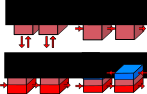
\includegraphics[width=\textwidth]{Thesis/drawing}
	\end{subfigure}
	\begin{subfigure}[b]{0.49\textwidth}
		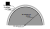
\includegraphics[width=\textwidth]{1DHemisphere/hemisphere2}
	\end{subfigure}
	\caption[Schematic for the various models and the domains used in the 1-Dimensional trials]{Left: Depictions of the four different blood transport models investigated in the 1-Dimensional trials. Pennes Bioheat Equation does not incorporate an advection term but instead assumes blood is directly delivered to each voxel. The Wulff/Klinger model assumes there is directional flow of blood between voxels and that blood is assumed to be equal to the tissue temperature. The Porous Two Phase Model divides each voxel into two parts with two temperatures, one for blood and one for the tissue. These two domains exchange heat between them however, the advection only occurs in the blood domain. The Counter-Current Model operates similarly but with each voxel divided into three, with one tissue domain and two blood domains that flow in opposite directions to each-other. As before, these two blood domains exchange heat with the tissue domain but do not interact with each other.  Right: Hemisphere domain used in 1-Dimensional trials.}
	\label{fig:1DHemisphere}
\end{figure}

Figure~\ref{fig:1DHemisphere} (right) displays a schematic of the domain used for these trials. When referring to the centre or the core of the hemisphere, the centre of base is intended rather than the geometric centroid of the shape. The surrounding scalp, skull and cerebral spinal fluid (CSF) regions depicted are not modelled but are instead used in calculating the surface heat flux.  

\subsubsection{Pennes Bioheat Equation}

Assuming the domain is homogeneous with full rotational symmetry, the spherical form of Pennes Bioheat Equation in the radial direction, $r$, is written as:

\begin{equation}
\rho c\frac{\partial T}{\partial t} = K\frac{1}{r^{2}}\frac{\partial}{\partial r}\bigg(r^{2}\frac{\partial T}{\partial r}\bigg)-c_{b}\overline{\omega}(T-T_{a}) + Q_{gen}
\end{equation}

With the bar in $\overline{\omega}$ denoting the total perfusion for the head, meaning the perfusion here is a single averaged value throughout the model. One temporal and two spatial boundary conditions are required to bound the system properly, one located at the centre of the hemisphere and the other at the surface. The boundary conditions used are steady-state, an adiabatic centre and a heat flux on the surface.

\begin{gather}
\frac{\partial T}{\partial t} = 0 \\
\frac{\partial T}{\partial r}\biggr|_{r=0} 	= 0 \\
K\frac{\partial T}{\partial r}\biggr|_{r=R} = h_{out}(T_{out}-T)\bigr|_{r=R}
\end{gather}

Where $r=0$ refers to the centre of the hemisphere and $r=R$ refers to the surface of the brain tissue. The variable, $h_{out}$, represents the surface heat transfer coefficient for the head model and $T_{out}$ is the environmental temperature at the surface.

\subsubsection{Wulff/Klinger Model}

The Wulff/Klinger equation in spherical form, in the radial direction, $r$, is written as:

\begin{equation}
\rho c\frac{\partial T}{\partial t} = K\frac{1}{r^{2}}\frac{\partial}{\partial r}\bigg(r^{2}\frac{\partial T}{\partial r}\bigg)-\rho_{b}c_{b}\bigg(\frac{1}{r^{2}}\frac{\partial}{\partial r}(r^{2}U_{r}T) \bigg) + Q_{gen}
\end{equation}

The superficial radial velocity, $U_{r}$, at $r$ within the hemisphere domain is:

\begin{equation}
U_{r} = \pm\frac{\overline{F}}{2\pi r^{2}\rho_{b}}
\label{Eq:SphericalVelocity}
\end{equation}

For a given overall blood mass flowrate, $\overline{F}$. The direction of flow is positive when blood flow is flowing towards the surface of the hemisphere and negative when the blood is directed towards the centre. 

The same boundary conditions are used as above with an additional source flux term added to the inlet. If flow is directed inwardly from the surface, the boundary conditions become:

\begin{gather}
\frac{\partial T}{\partial t} = 0 \\
\frac{\partial T}{\partial r}\biggr|_{r=0} = 0 \\
K\frac{\partial T}{\partial r}\biggr|_{r=R} = h_{out}(T_{out}-T)\bigr|_{r=R} + \frac{c_{b}\overline{F}}{2\pi R^{2}}(T_{a} - T)\bigr|_{r=R}
\end{gather}

If the flow direction is outward, then there is a singularity when determining velocity in Equation~\ref{Eq:SphericalVelocity} at the core where $\lim_{r\to0}$ and the source flux approaches infinity. To avoid this, instead of an adiabatic core, the temperature at the centre is assumed to equal the arterial blood temperature. Therefore, the boundary conditions are:

\begin{gather}
\frac{\partial T}{\partial t} = 0 \\
T\bigr|_{r=0}=T_{a} \\
\bigg(K\frac{\partial T}{\partial r} - \rho_{b}c_{b}\int_{r-\Delta r}^{r}\bigg(\frac{1}{r^{2}}\frac{\partial}{\partial r}(r^{2}U_{r}T)\partial r\bigg)\bigg)\biggr|_{r=R} = h_{out}(T_{out}-T)\bigr|_{r=R}
\end{gather}

\subsubsection{Porous Two Phase Model}

For a porous system, there are two phases within the hemisphere, a solid phase and a fluid phase that represent the tissue and blood respectively. Therefore, there are two sets of heat equations which include an inter-phase heat transfer term. As the two domains occupy the same space, a volume fraction, or porosity, $\epsilon$, has to be defined. The tissue phase volume fraction is given in terms of the blood phase volume fraction by $\epsilon=1-\epsilon_{b}$ and vice versa. For these trials, these terms are homogeneous constants. Equations~\ref{Eq:TissueSpherical}~\&~\ref{Eq:BloodSpherical} represent the spherical equations in the radial direction, $r$, for the tissue and blood phases respectively.

\begin{equation}
\epsilon\rho c\frac{\partial T}{\partial t} = \epsilon K\frac{1}{r^{2}}\frac{\partial}{\partial r}\bigg(r^{2}\frac{\partial T}{\partial r}\bigg) + h_{bt}\alpha_{bt}(T_{b}-T) + Q_{gen}
\label{Eq:TissueSpherical}
\end{equation}

\begin{equation}
\epsilon_{b}\rho_{b}c_{b}\frac{\partial T_{b}}{\partial t} = \epsilon_{b}K_{b}\frac{1}{r^{2}}\frac{\partial}{\partial r}\bigg(r^{2}\frac{\partial T_{b}}{\partial r}\bigg)-\rho_{b}c_{b}\bigg(\frac{1}{r^{2}}\frac{\partial}{\partial r}(r^{2}U_{r}T_{b}) \bigg)-h_{bt}\alpha_{bt}(T_{b}-T)
\label{Eq:BloodSpherical}
\end{equation}

Here, the terms $h_{bt}$ and $\alpha_{bt}$ represent respectively the surface heat transfer coefficient and specific surface area between the blood and tissue phases in the porous media. The same superficial velocity defined in Equation~\ref{Eq:SphericalVelocity} is used in Equation~\ref{Eq:BloodSpherical}. For the tissue phase, the steady-state, adiabatic centre, and surface heat flux boundary conditions are equivalent to the those used with the Pennes Bioheat Equation:

\begin{gather}
\frac{\partial T}{\partial t} = 0 \\
\frac{\partial T}{\partial r}\biggr|_{r=0} = 0 \\
K\frac{\partial T}{\partial r}\biggr|_{r=R} = h_{out}(T_{out}-T)\bigr|_{r=R}
\end{gather}

For the blood phase, the boundary conditions are equivalent to the boundary conditions used for the Wulff/Klinger Equation with the inclusion of the porosity term. For inward flow: 

\begin{gather}
\frac{\partial T_{b}}{\partial t} = 0 \\
\frac{\partial T_{b}}{\partial r}\biggr|_{r=0} = 0 \\
\epsilon_{b}K_{b}\frac{\partial T_{b}}{\partial r}\biggr|_{r=R} = \epsilon_{b}h_{out}(T_{out}-T_{b})\bigr|_{r=R} + \frac{c_{b}\overline{F}}{2\pi R^{2}}(T_{a} - T_{b})\bigr|_{r=R}
\end{gather}

And outward flow:

\begin{gather}
\frac{\partial T_{b}}{\partial t} = 0 \\
T_{b}\bigr|_{r=0} = T_{a} \\
\bigg(\epsilon_{b}K_{b}\frac{\partial T_{b}}{\partial r} - \rho_{b}c_{b}\int_{r-\Delta r}^{r}\bigg(\frac{1}{r^{2}}\frac{\partial}{\partial r}(r^{2}U_{r}T_{b})\partial r\bigg)\bigg)\biggr|_{r=R} = \epsilon_{b}h_{out}(T_{out}-T_{b})\bigr|_{r=R}
\end{gather}

On top of this, two extra parameters need to be defined in this situation, the inter-domain heat transfer parameters and the porosity.

Equations~\ref{Eq:TissueSpherical}~\&~\ref{Eq:BloodSpherical} can be reduced to both the Wulff/Klinger model and the Pennes Bioheat Equations under certain conditions. If the physical parameters of tissue and blood are assumed to be the same ($\rho=\rho_{b}$ \& $c=c_{b}$), and the inter-phase heat transfer is assumed to be infinite ($\lim_{h_{bt}\alpha_{bt}\to\infty}: T_{t}=T_{b}$) then the porous model operates equivalently to the Wulff/Klinger model. If in the porous model, $c_{b}$ is considered infinite and the initial condition $T_{b} = T_{a}$ is used, the porous model performs equivalently to the Pennes Bioheat Equation if $h_{bt}\alpha_{bt} = c_{b}\overline{\omega}$ where, here, $c_{b}$ equals its original physical value. Therefore, there are two cases for inter-domain heat transfer: one where there the blood and tissue reach an equilibrium instantaneously with $h_{bt}\alpha_{bt}=\infty$ and another where there is a fixed magnitude for the inter-domain heat transfer with $h_{bt}\alpha_{bt} = c_{b}\overline{\omega}$.

The porosity was estimated using values for cerebral blood volume obtained in literature \cite{larsson2009measurement}. Although, it is expected that, except in extreme cases, the porosity should not have much effect on the results. The physical parameters for the two phases are very similar meaning there would not be a large shift in specific energy of the system with varying porosity. 

\subsubsection{Counter-Current Model}

By splitting the fluid domain into two non-interacting fluid domains, counter-current blood flow can be simulated with the corresponding heat transfer. The equations used for this model are shown below:

\begin{equation}
\epsilon\rho c\frac{\partial T}{\partial t} = \epsilon K\frac{1}{r^{2}}\frac{\partial}{\partial r}\bigg(r^{2}\frac{\partial T}{\partial r}\bigg) + h_{bt}\alpha_{bt}(T_{b1}-T) + h_{bt}\alpha_{bt}(T_{b2}-T) + Q_{gen}
\label{Eq:TissueSphericalXR}
\end{equation}

\begin{equation}
\epsilon_{b}\rho_{b}c_{b}\frac{\partial T_{b1}}{\partial t} = \epsilon_{b}K_{b}\frac{1}{r^{2}}\frac{\partial}{\partial r}\bigg(r^{2}\frac{\partial T_{b1}}{\partial r}\bigg)-\rho_{b}c_{b}\bigg(\frac{1}{r^{2}}\frac{\partial}{\partial r}(r^{2}U_{r}T_{b1}) \bigg)-h_{bt}\alpha_{bt}(T_{b1}-T)
\label{Eq:BloodSphericalXR1}
\end{equation}

\begin{equation}
\epsilon_{b}\rho_{b}c_{b}\frac{\partial T_{b2}}{\partial t} = \epsilon_{b}K_{b}\frac{1}{r^{2}}\frac{\partial}{\partial r}\bigg(r^{2}\frac{\partial T_{b2}}{\partial r}\bigg)-\rho_{b}c_{b}\bigg(\frac{1}{r^{2}}\frac{\partial}{\partial r}(r^{2}(-U_{r})T_{b2}) \bigg)-h_{bt}\alpha_{bt}(T_{b2}-T)
\label{Eq:BloodSphericalXR2}
\end{equation}

With $T_{b1}$ and $T_{b1}$ being the temperatures of the two distinct blood phases. All physical properties in the blood domains can be assumed to be equal. As the blood domain has doubled in volume, the tissue porosity becomes $\epsilon = 1 - 2\epsilon_{b}$ to compensate. 

The inter-domain heat transfer is assumed to only occur between tissue and blood domains as the vessels are assumed never to be in contact. Similar values for the $h_{bt}\alpha_{bt}$ term can be used as in the single-blood domain model. However, the model breaks down at high inter-domain heat transfer as $T$, $T_{b1}$, \& $T_{b2}$ become equal. In this instance, the equations can be reduced to a single equation, such as before with the Wulff model. However, the velocity terms cancel out as they flow in opposite directions. This removes the advection completely from the model and it behaves as a purely conductive model instead. 

The boundary conditions for the tissue are similar to the uni-directional two-phase model:  

\begin{gather}
\frac{\partial T}{\partial t} = 0 \\
\frac{\partial T}{\partial r}\biggr|_{r=0} = 0 \\
K\frac{\partial T}{\partial r}\biggr|_{r=R} = h_{out}(T_{out}-T)\bigr|_{r=R}
\end{gather}

The blood flow is considered to originate from the centre of the model in the first phase ($b1$) and to return there in the second phase ($b2$). The boundary conditions for $b1$ are then: 

\begin{gather}
\frac{\partial T_{b1}}{\partial t} = 0 \\
T_{b1}\bigr|_{r=0} = T_{a} \\
\bigg(\epsilon_{b}K_{b}\frac{\partial T_{b1}}{\partial r} -\rho_{b}c_{b}\int_{r-\Delta r}^{r}\bigg(\frac{1}{r^{2}}\frac{\partial}{\partial r}(r^{2}U_{r}T_{b1})\partial r\bigg)\bigg)\biggr|_{r=R} = \epsilon_{b}h_{out}(T_{out}-T_{b1})\bigr|_{r=R}
\end{gather}

And for $b2$:

\begin{gather}
\frac{\partial T_{b2}}{\partial t} = 0 \\
\frac{\partial T_{b2}}{\partial r}\biggr|_{r=0} = 0 \\
\epsilon_{b}K_{b}\frac{\partial T_{b2}}{\partial r}\biggr|_{r=R} = \epsilon_{b}h_{out}(T_{out}-T_{b2})\bigr|_{r=R} + \frac{c_{b}\overline{F}}{2\pi R^{2}}(T_{b1} - T_{b2})\bigr|_{r=R}
\end{gather}

\subsection{Set-Up}

The radius of the hemisphere was set to $8.6cm$ which gives a cerebral volume of $\text{1,332}cm^{3}$, comparable to an adult brain \cite{hedman2012human} and the same size used by Nelson and Nunnely \cite{nelson1998brain}. The physical parameters used for the model are given in Table~\ref{tab:physicalparams}. The overall flowrate of blood, $\overline{F}$ can be calculated using the overall perfusion rate and the volume of tissue, giving $\overline{F} = 11.66g/s$. 

Two values for $h_{bt}\alpha_{bt}$ were used for the two-domain models. The first compares the Two Phase model to Pennes Bioheat Equation with $h_{bt}\alpha_{bt} = c_{b}\overline{\omega} = \text{34,914}W/m^{3}/^{o}C$ which is of the same order of magnitude to that used in Xuan \& Roetzel \cite{xuan1997bioheat} ($h_{bt} = 316.5 W/m^{2}/^{o}C$ and $\alpha_{bt} = 80m^{2}/m^{3}$ which give a value of $h_{bt}\alpha_{bt} = \text{25,320} W/m^{3}/^{o}C$). The other compares the Two Phase model to the Wulff/Klinger Equation by setting the inter-domain heat transfer to an arbitrary large value, $h_{bt}\alpha_{bt} = 10^8W/m^{3}/^{o}C$.

\begin{table}
	\centering
	\fontsize{8pt}{9pt}\selectfont
	\begin{tabular}{p{5.0cm} c c}
		\toprule
		\textbf{Physical Parameter} & \textbf{Value} & \textbf{Units}\\ \hline
		Density, $\rho$ & &\\
		\qquad Tissue & 1050$^{\dagger}$ & $kg/m^{3}$ \\ 
		\qquad Blood & 1050$^{\dagger}$ & $kg/m^{3}$ \\ 
		Thermal Conductivity, $K$ & &\\
		\qquad Tissue & 0.5$^{\dagger}$ & $W/m/^{o}C$ \\ 
		\qquad Blood & 0.492$^{\dagger}$ & $W/m/^{o}C$ \\
		Specific Heat Capacity. $c$  & &\\
		\qquad Tissue & 3700$^{\dagger}$ & $J/kg/^{o}C$ \\ 
		\qquad Blood & 3800$^{\dagger}$ & $J/kg/^{o}C$ \\
		Blood Volume Fraction, $\epsilon_{b}$ & 0.05$^{\ddagger}$ & - \\
		Overall Perfusion Rate, $\overline{\omega}$ & 9.188$^{\dagger}$ & $kg/m^{3}/s$ \\
		Metabolic Heat Generation, $Q_{gen}$ & 10,437$^{\dagger}$ & $W/m^{3}$ \\
		Arterial Blood Temperature, $T_{a}$ & 37$^{\dagger}$ & $^{o}C$ \\ \bottomrule
	\end{tabular}
	
	\caption[Table of physical parameters used in 1-Dimensional radial model]{Table of physical parameters used in 1-Dimensional radial model. $^{\dagger}$Zhu and Diao \cite{zhu2001theoretical}. $^{\ddagger}$Estimated from cerebral blood volumes taken from Larsson et al. \cite{larsson2009measurement}.}
	\label{tab:physicalparams}
\end{table}

The temperature boundary condition at the surface is a set scalp temperature, $T_{scalp}$. This avoids assuming a value for surface heat transfer coefficient for the scalp which is a generally assumed parameter \cite{nelson1998brain,xuan1997bioheat}. The heat flux from the brain surface is calculated using the scalp temperature and the sum of the resistances, $\Omega$, of the various tissues between the scalp and the brain. For a hemispherical system these are given as:

\begin{equation}
\Omega = \sum_{z}\Omega_{z}=\sum\frac{r_{z2}-r_{z1}}{2\pi r_{z2}r_{z1}K_{z}}
\end{equation}

Where $r_{z1}$ and $r_{z2}$ are the radii that bound a portion of surface tissue, $z$. Using the values provided in Table~\ref{tab:heattransfercoeff} gives an overall resistance of $2.42^{o}C/W$ or a surface heat transfer coefficient, $h_{out}=52.1W/m^{2}/^{o}C$, at the brain surface, $r = 8.6cm$. Two scalp temperatures were chosen to represent normal conditions and extreme cooling. Normal scalp temperature is assumed to be $36.5^{o}C$ and for the cooling scenario, the scalp temperature was assumed to be $10^{o}C$.

\begin{table}
	\centering
	\fontsize{8pt}{9pt}\selectfont
	\begin{tabular}{c c c}
		\toprule
		\textbf{Tissue Type} & \textbf{Thermal Conductivity, $K_{z}$} & \textbf{Thickness, $r_{z2}-r_{z1}$} \\ \hline
		CSF & 0.582$W/m/^{o}C$ & $2mm$ \\ 
		Skull & 1.16$W/m/^{o}C$ & $5mm$ \\ 
		Scalp & 0.340$W/m/^{o}C$ & $5mm$ \\ \bottomrule
	\end{tabular}
	\caption[Surface heat transfer properties of a human head]{Table of surface heat transfer properties of a human head. Found in Nelson and Nunneley \cite{nelson1998brain}.}
	\label{tab:heattransfercoeff}
\end{table}

The equations were discretised on a grid of 502 points and were solved as a linear system in the form of:

\begin{equation}
\mathbf{A}\mathbf{x}=\mathbf{B}
\end{equation}

Where $\mathbf{A}$ is a matrix of the coefficients, $\mathbf{x}$ is a vector containing the values for temperature at each point of the system and $\mathbf{B}$ is a vector of constants. Doubling the number of grid points showed changes of less than 1\% to results.

\subsection{Results \& Discussion}
\label{Sec:21DHemisphereResults}

\begin{figure}[h]
	\centering
	\begin{subfigure}[b]{0.49\textwidth}
		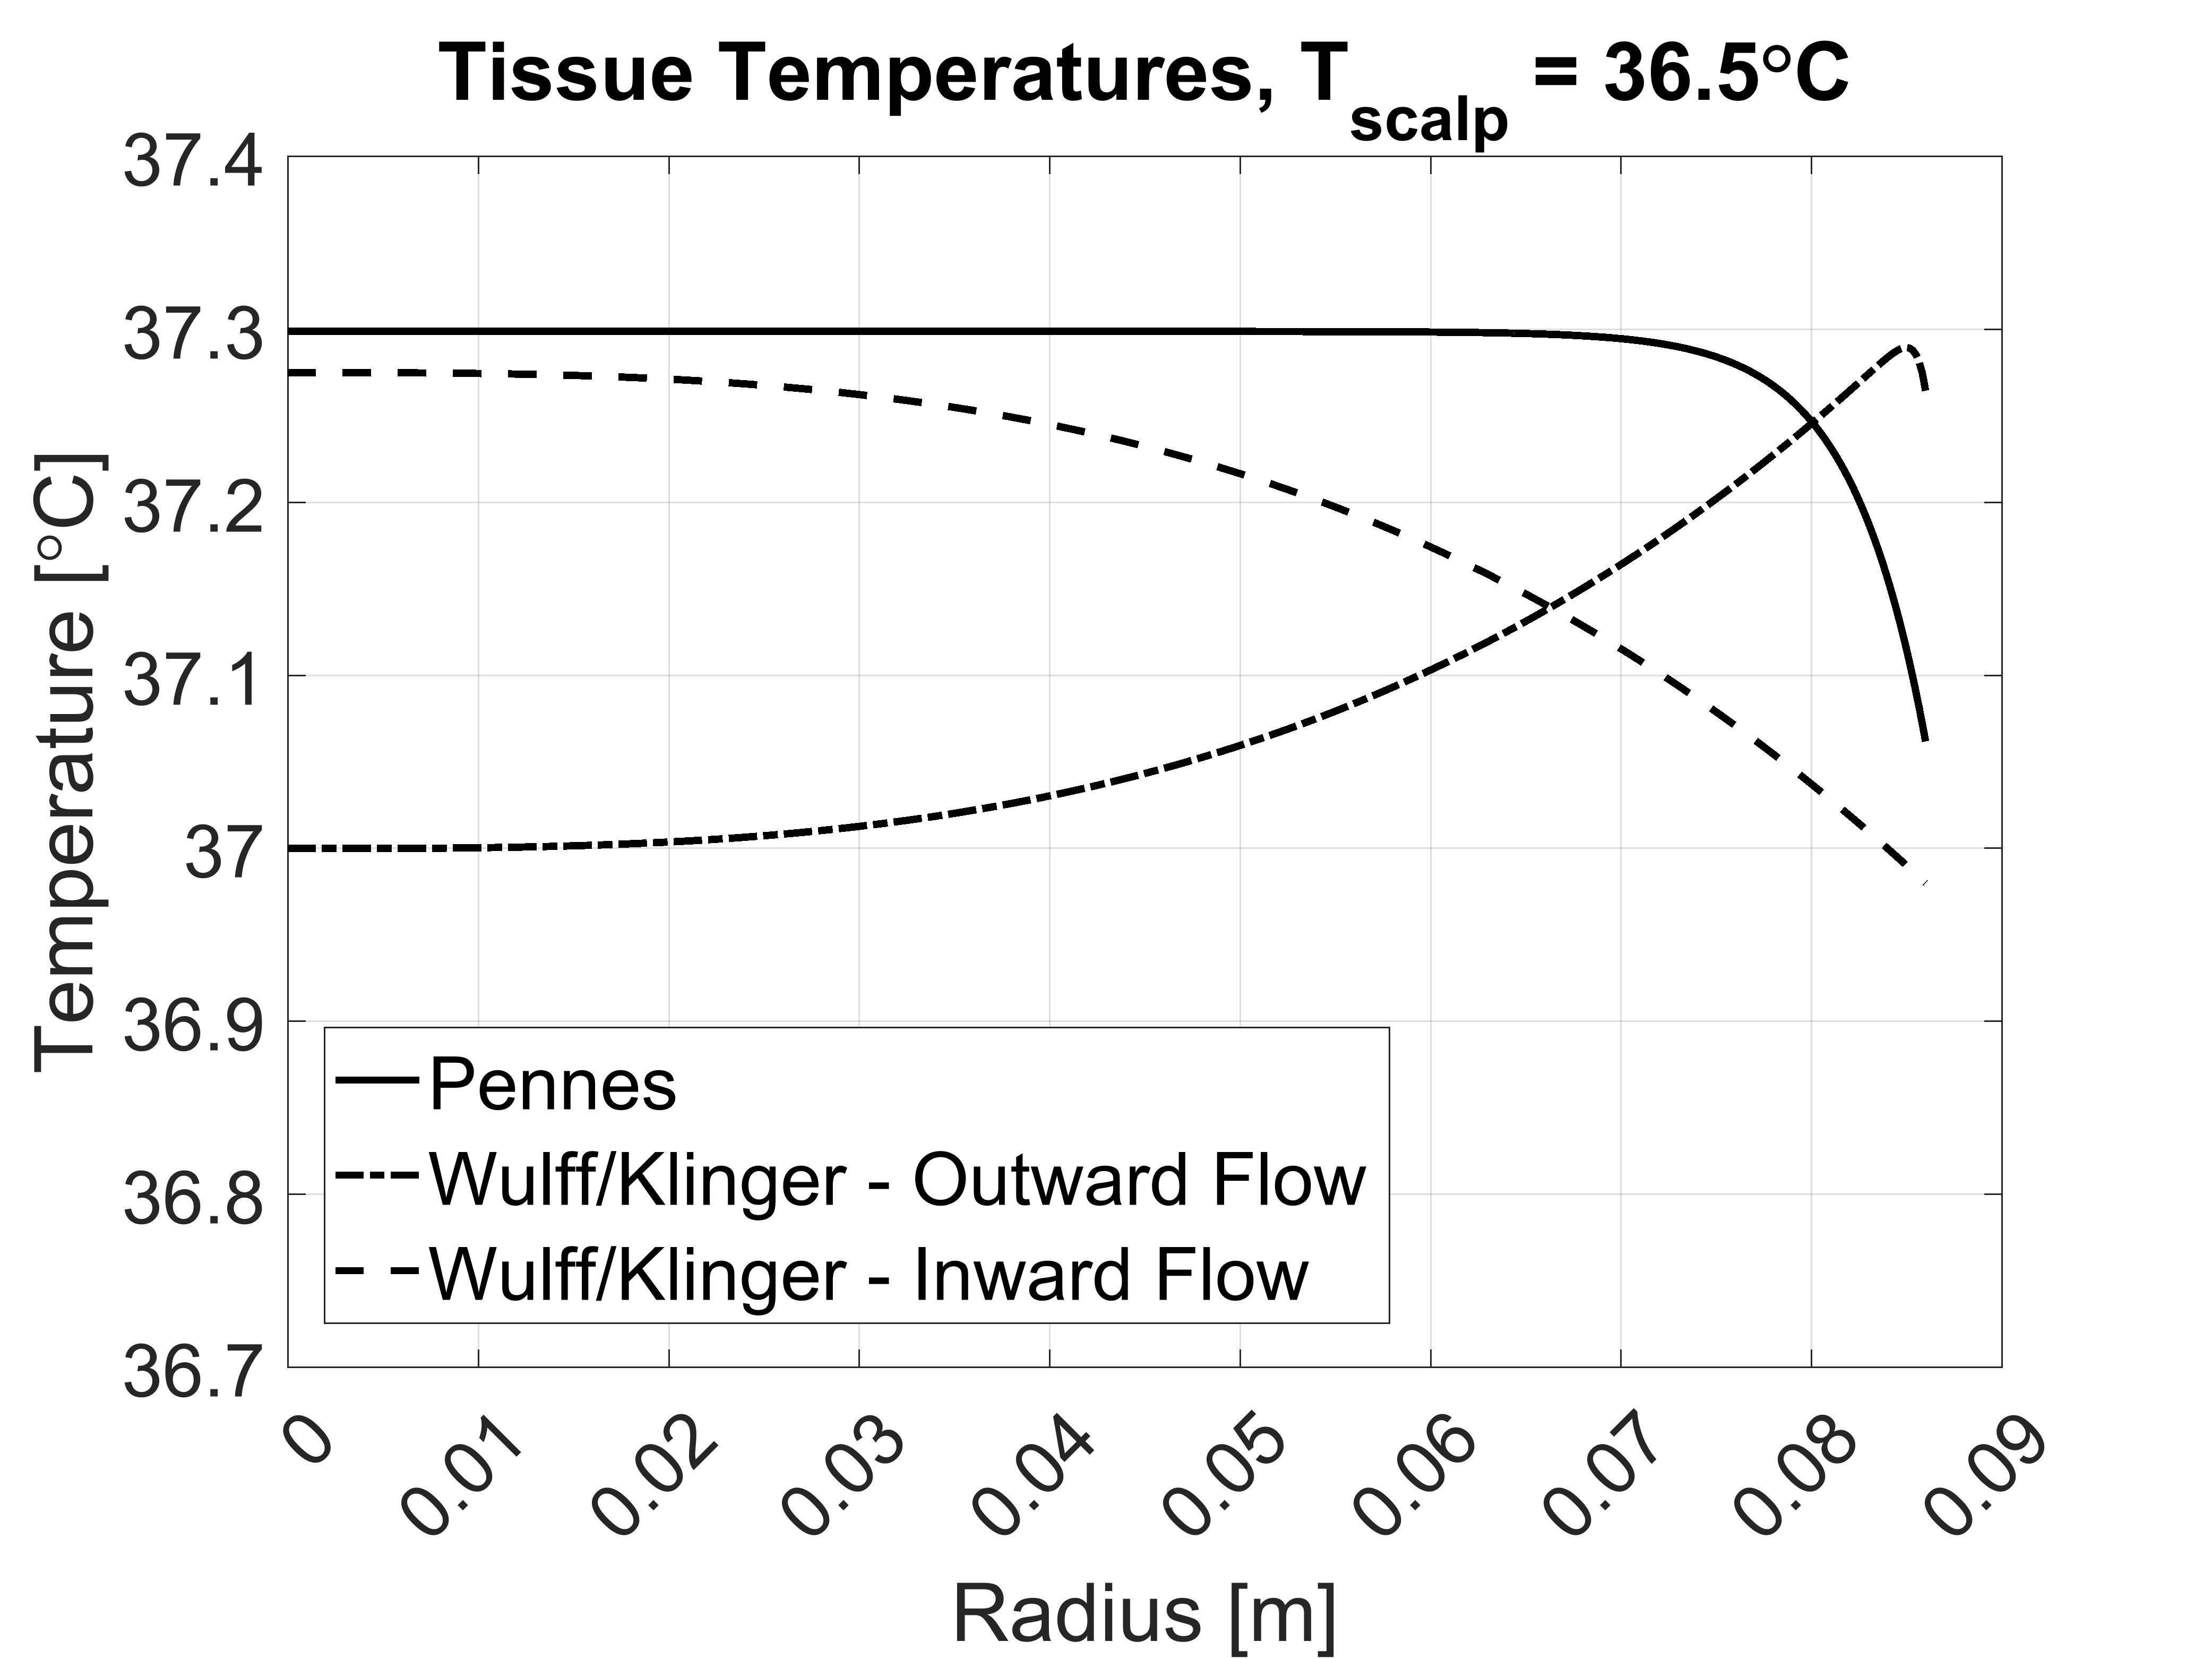
\includegraphics[width=\textwidth]{1DHemisphere/figure1}
	\end{subfigure}
	\begin{subfigure}[b]{0.49\textwidth}
		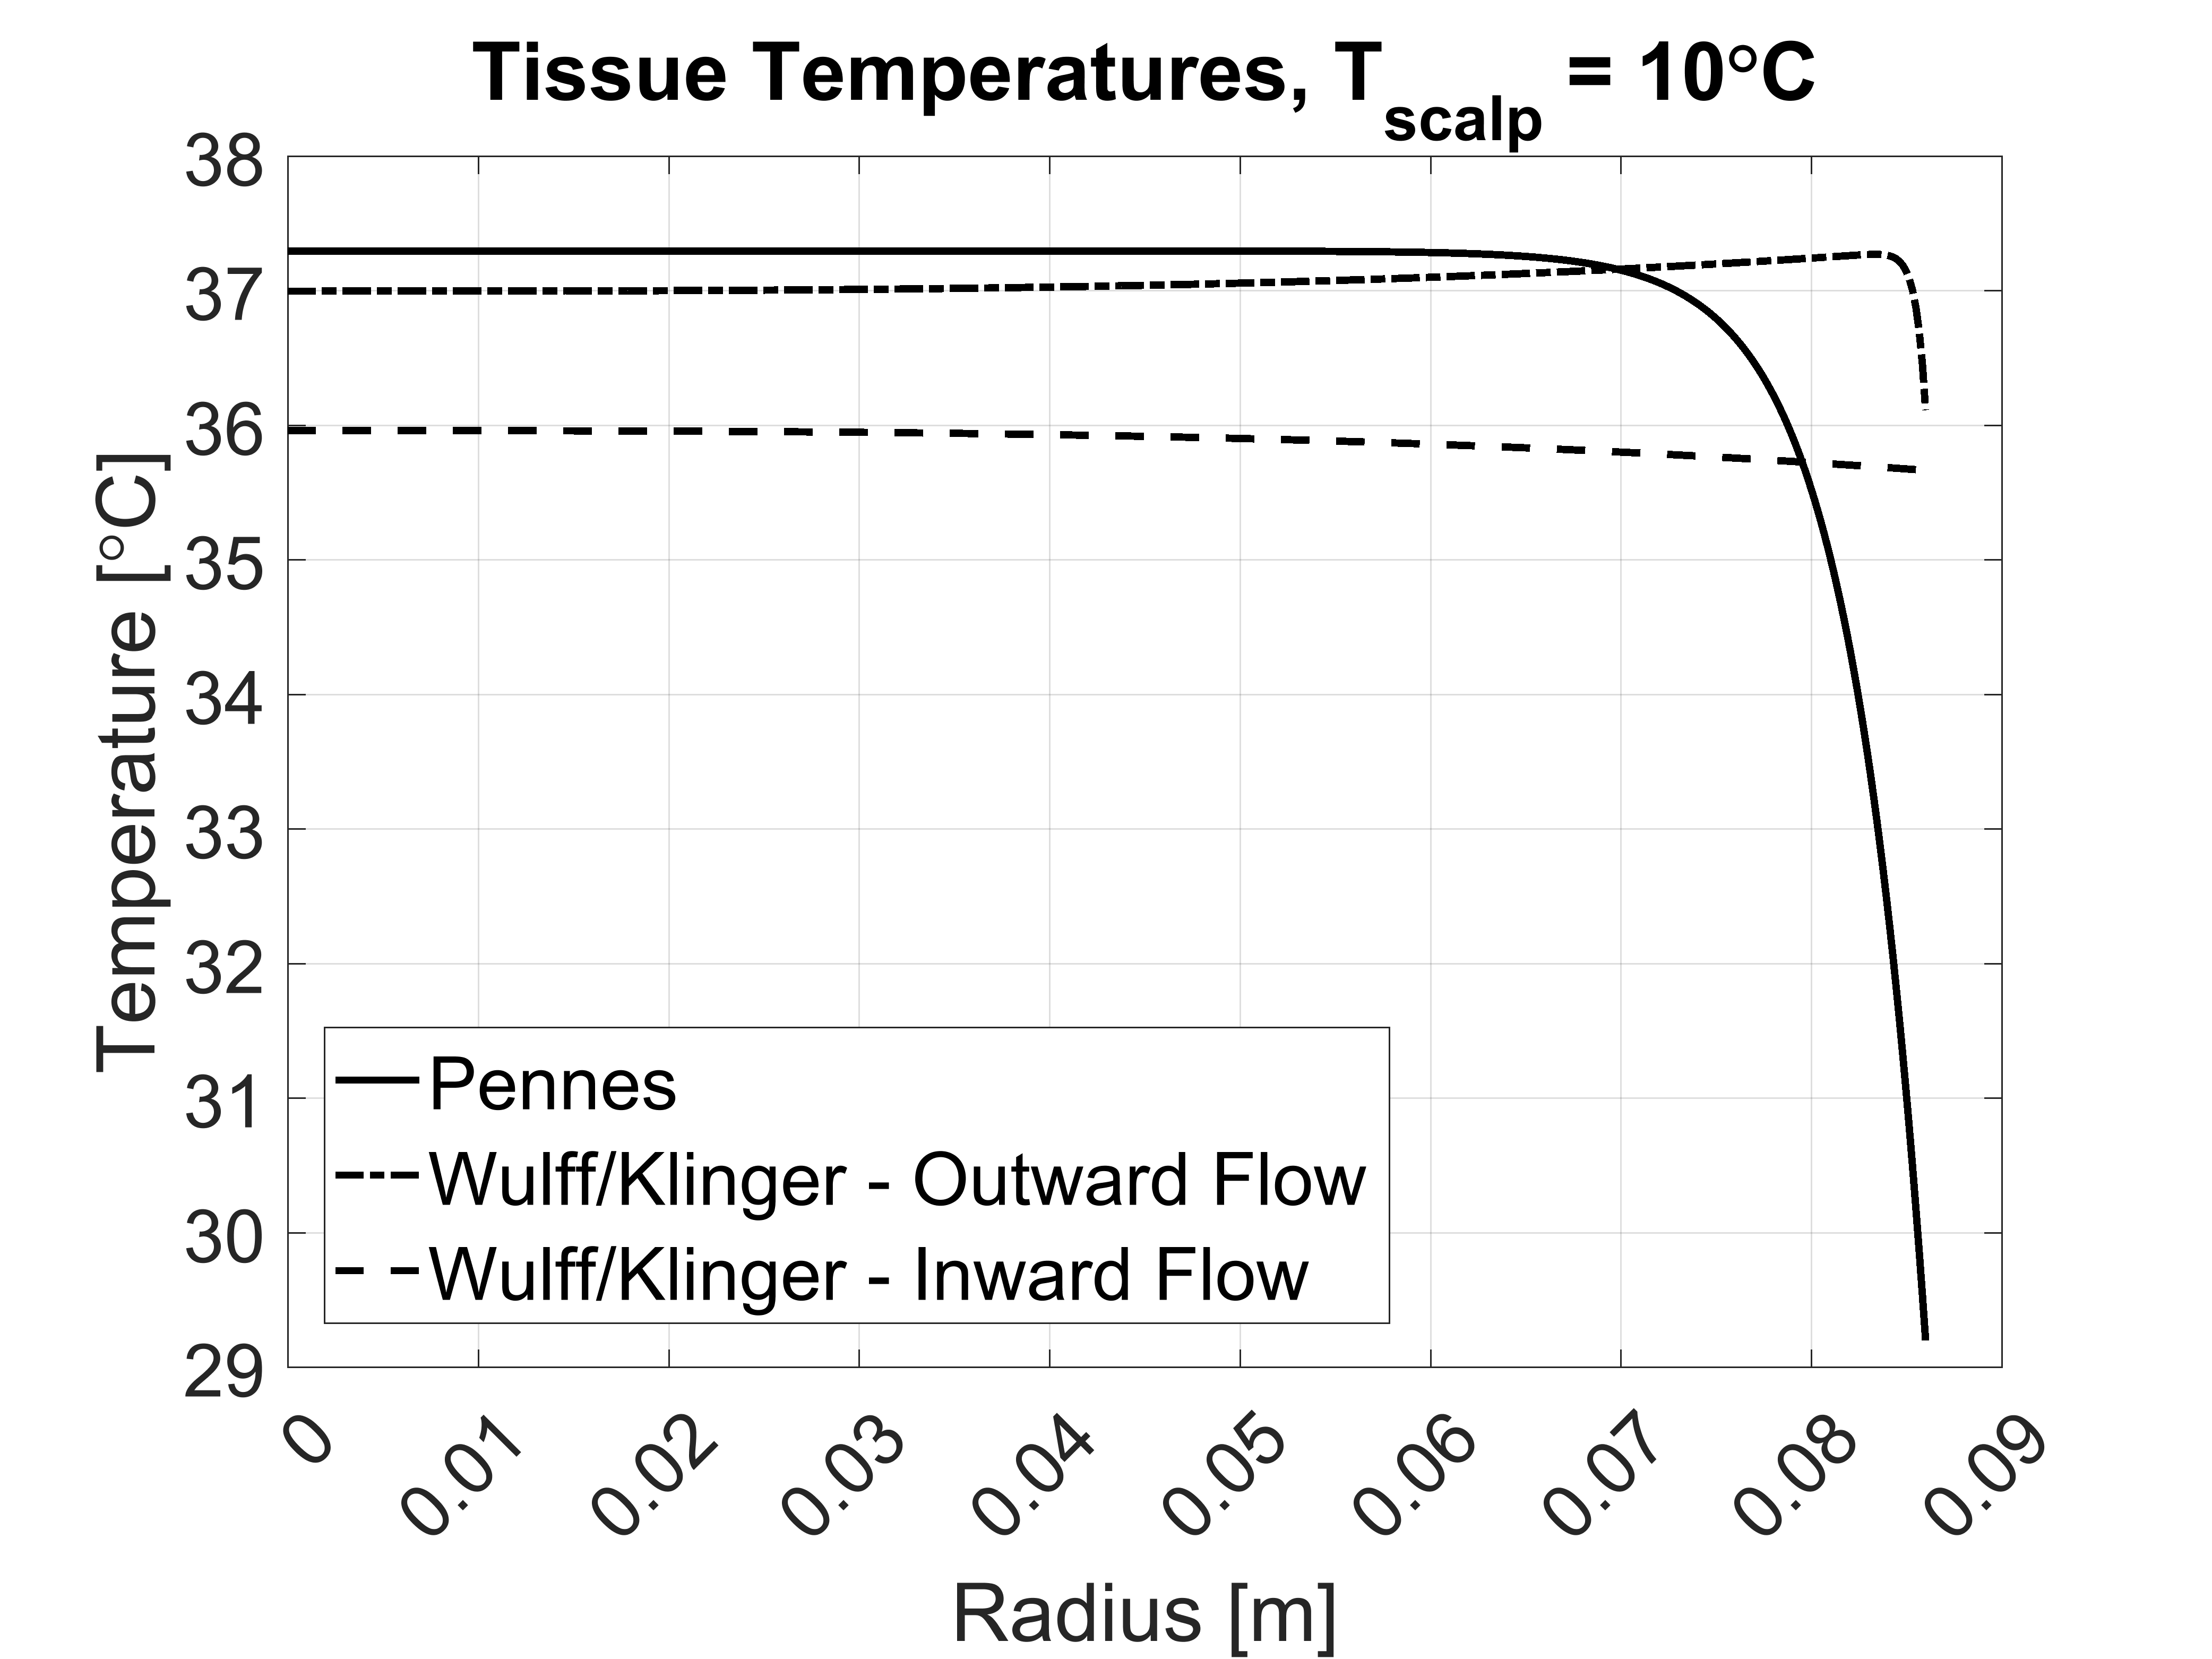
\includegraphics[width=\textwidth]{1DHemisphere/figure2}
	\end{subfigure}
	\caption[Radial temperature distributions for the Pennes Bioheat Equations and the Wulff/Klinger Equations for $T_{scalp}=36.5^{o}C$ and $T_{scalp}=10^{o}C$]{Radial temperature distributions for the Pennes Bioheat Equations and the Wulff/Klinger Equations for $T_{scalp}=36.5^{o}C$ (left) and $T_{scalp}=10^{o}C$ (right).}
	\label{fig:Results1}
\end{figure}

Figure~\ref{fig:Results1} shows the radial temperature profiles for the Pennes Bioheat Equations and Wulff/Klinger Equations under normal and cooling conditions. For Pennes Bioheat Equation, a large temperature gradient is present at the surface with a isothermal core temperature. This agrees with previous models and is the basis for the temperature shielding effect theory presented by Zhu et al. \cite{zhu2006body}. The Wulff/Klinger model shows a more varied profile for temperature throughout the model. This is the effect of including an advection term to represent the transport of blood instead of a perfusion source/sink term. Under normal conditions both the outward and inward flow directions display a lower average temperature, $37.15^{o}C$ and $37.13^{o}C$ respectively, compared to the Pennes Bioheat Equation average of $37.27^{o}C$. 

Ignoring boundary conditions, the tissue temperature in the Pennes Bioheat Equation should have a rise of $0.30^{o}C$ from arterial blood temperature due to the competition between the perfusion term and the metabolic heat generation ($\frac{\overline{Q}_{gen}}{c_{b}\overline{\omega}}=0.30^{o}C$). This can be observed in the Wulff/Klinger model too as the temperature increase steadily approaches this value as blood passes from inlet to outlet. However, contrastingly, the Wulff/Klinger model only peaks at this value whereas it is generally constant within the Pennes model. This highlights the difference in that the entire flowrate of blood is passing through each point within the Wulff/Klinger model while only portions of this flow are delivered to each point in the Pennes model. For inward flow in the Wulff/Klinger model, the peak temperature is slightly lower than the expected increase of $0.30^{o}C$ as the blood is initially cooled from the surface conditions. 

\begin{figure}[h]
	\centering
	\begin{subfigure}[b]{0.49\textwidth}
		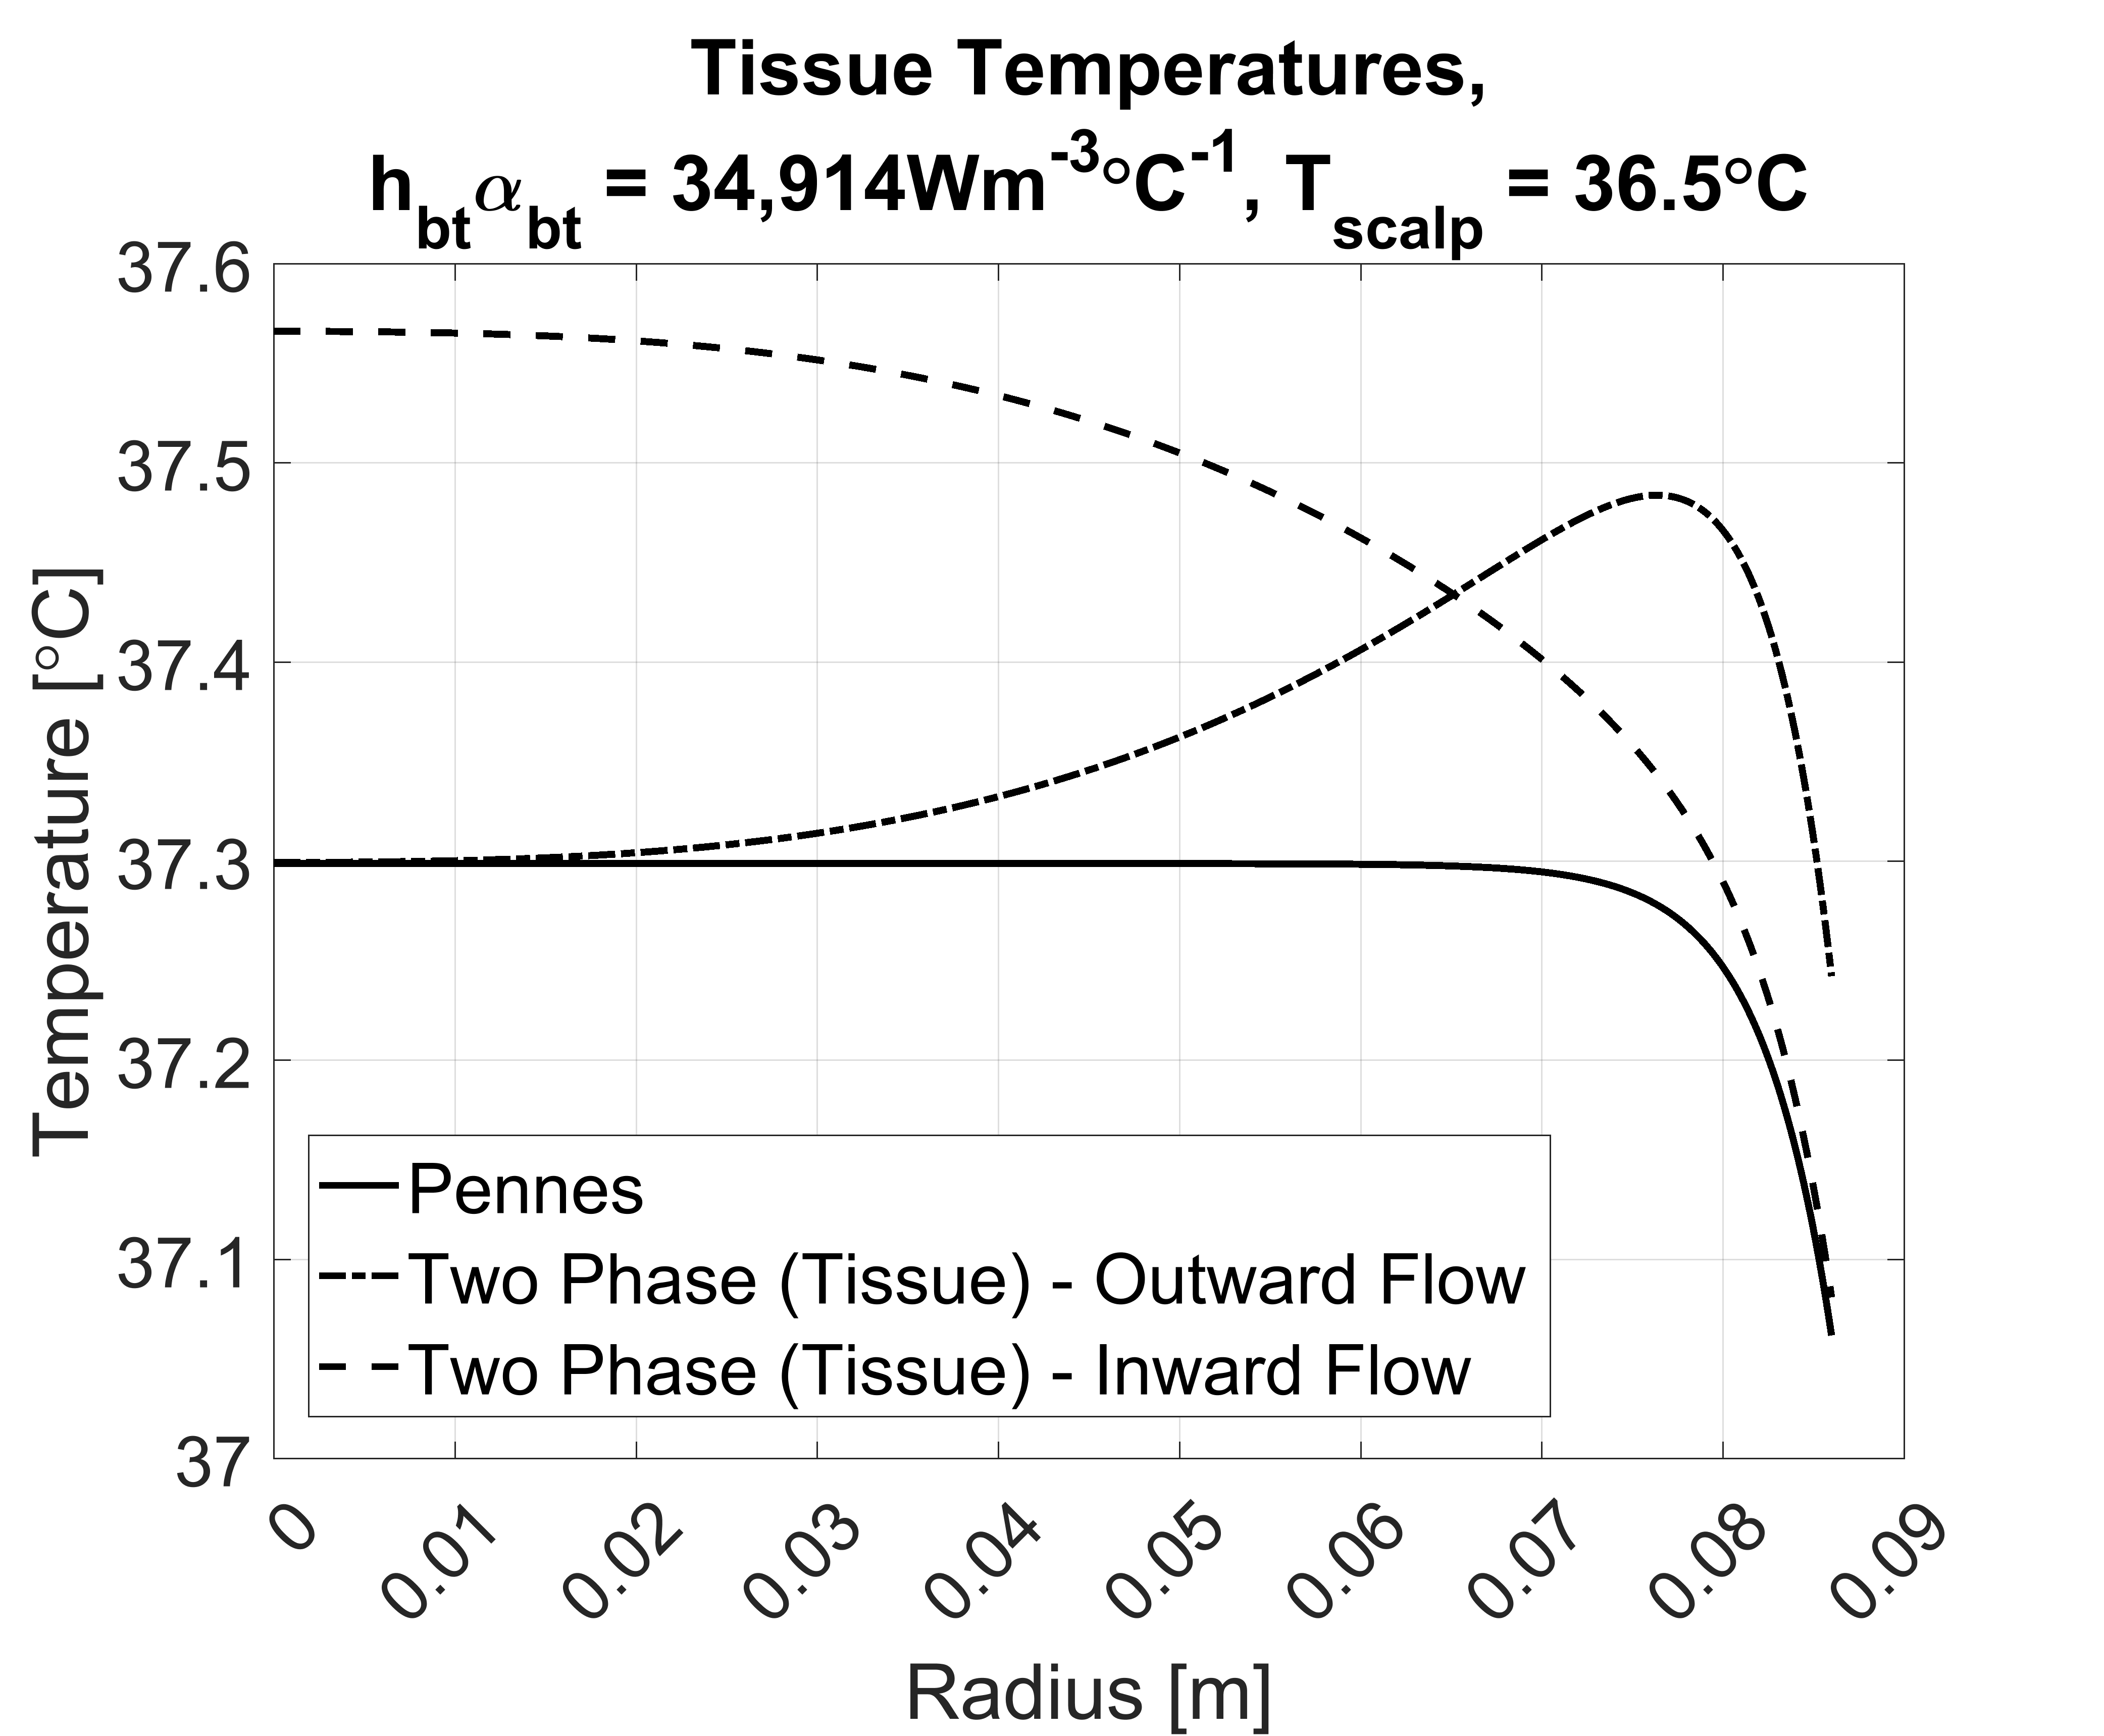
\includegraphics[width=\textwidth]{1DHemisphere/figure3}
	\end{subfigure}
	\begin{subfigure}[b]{0.49\textwidth}
		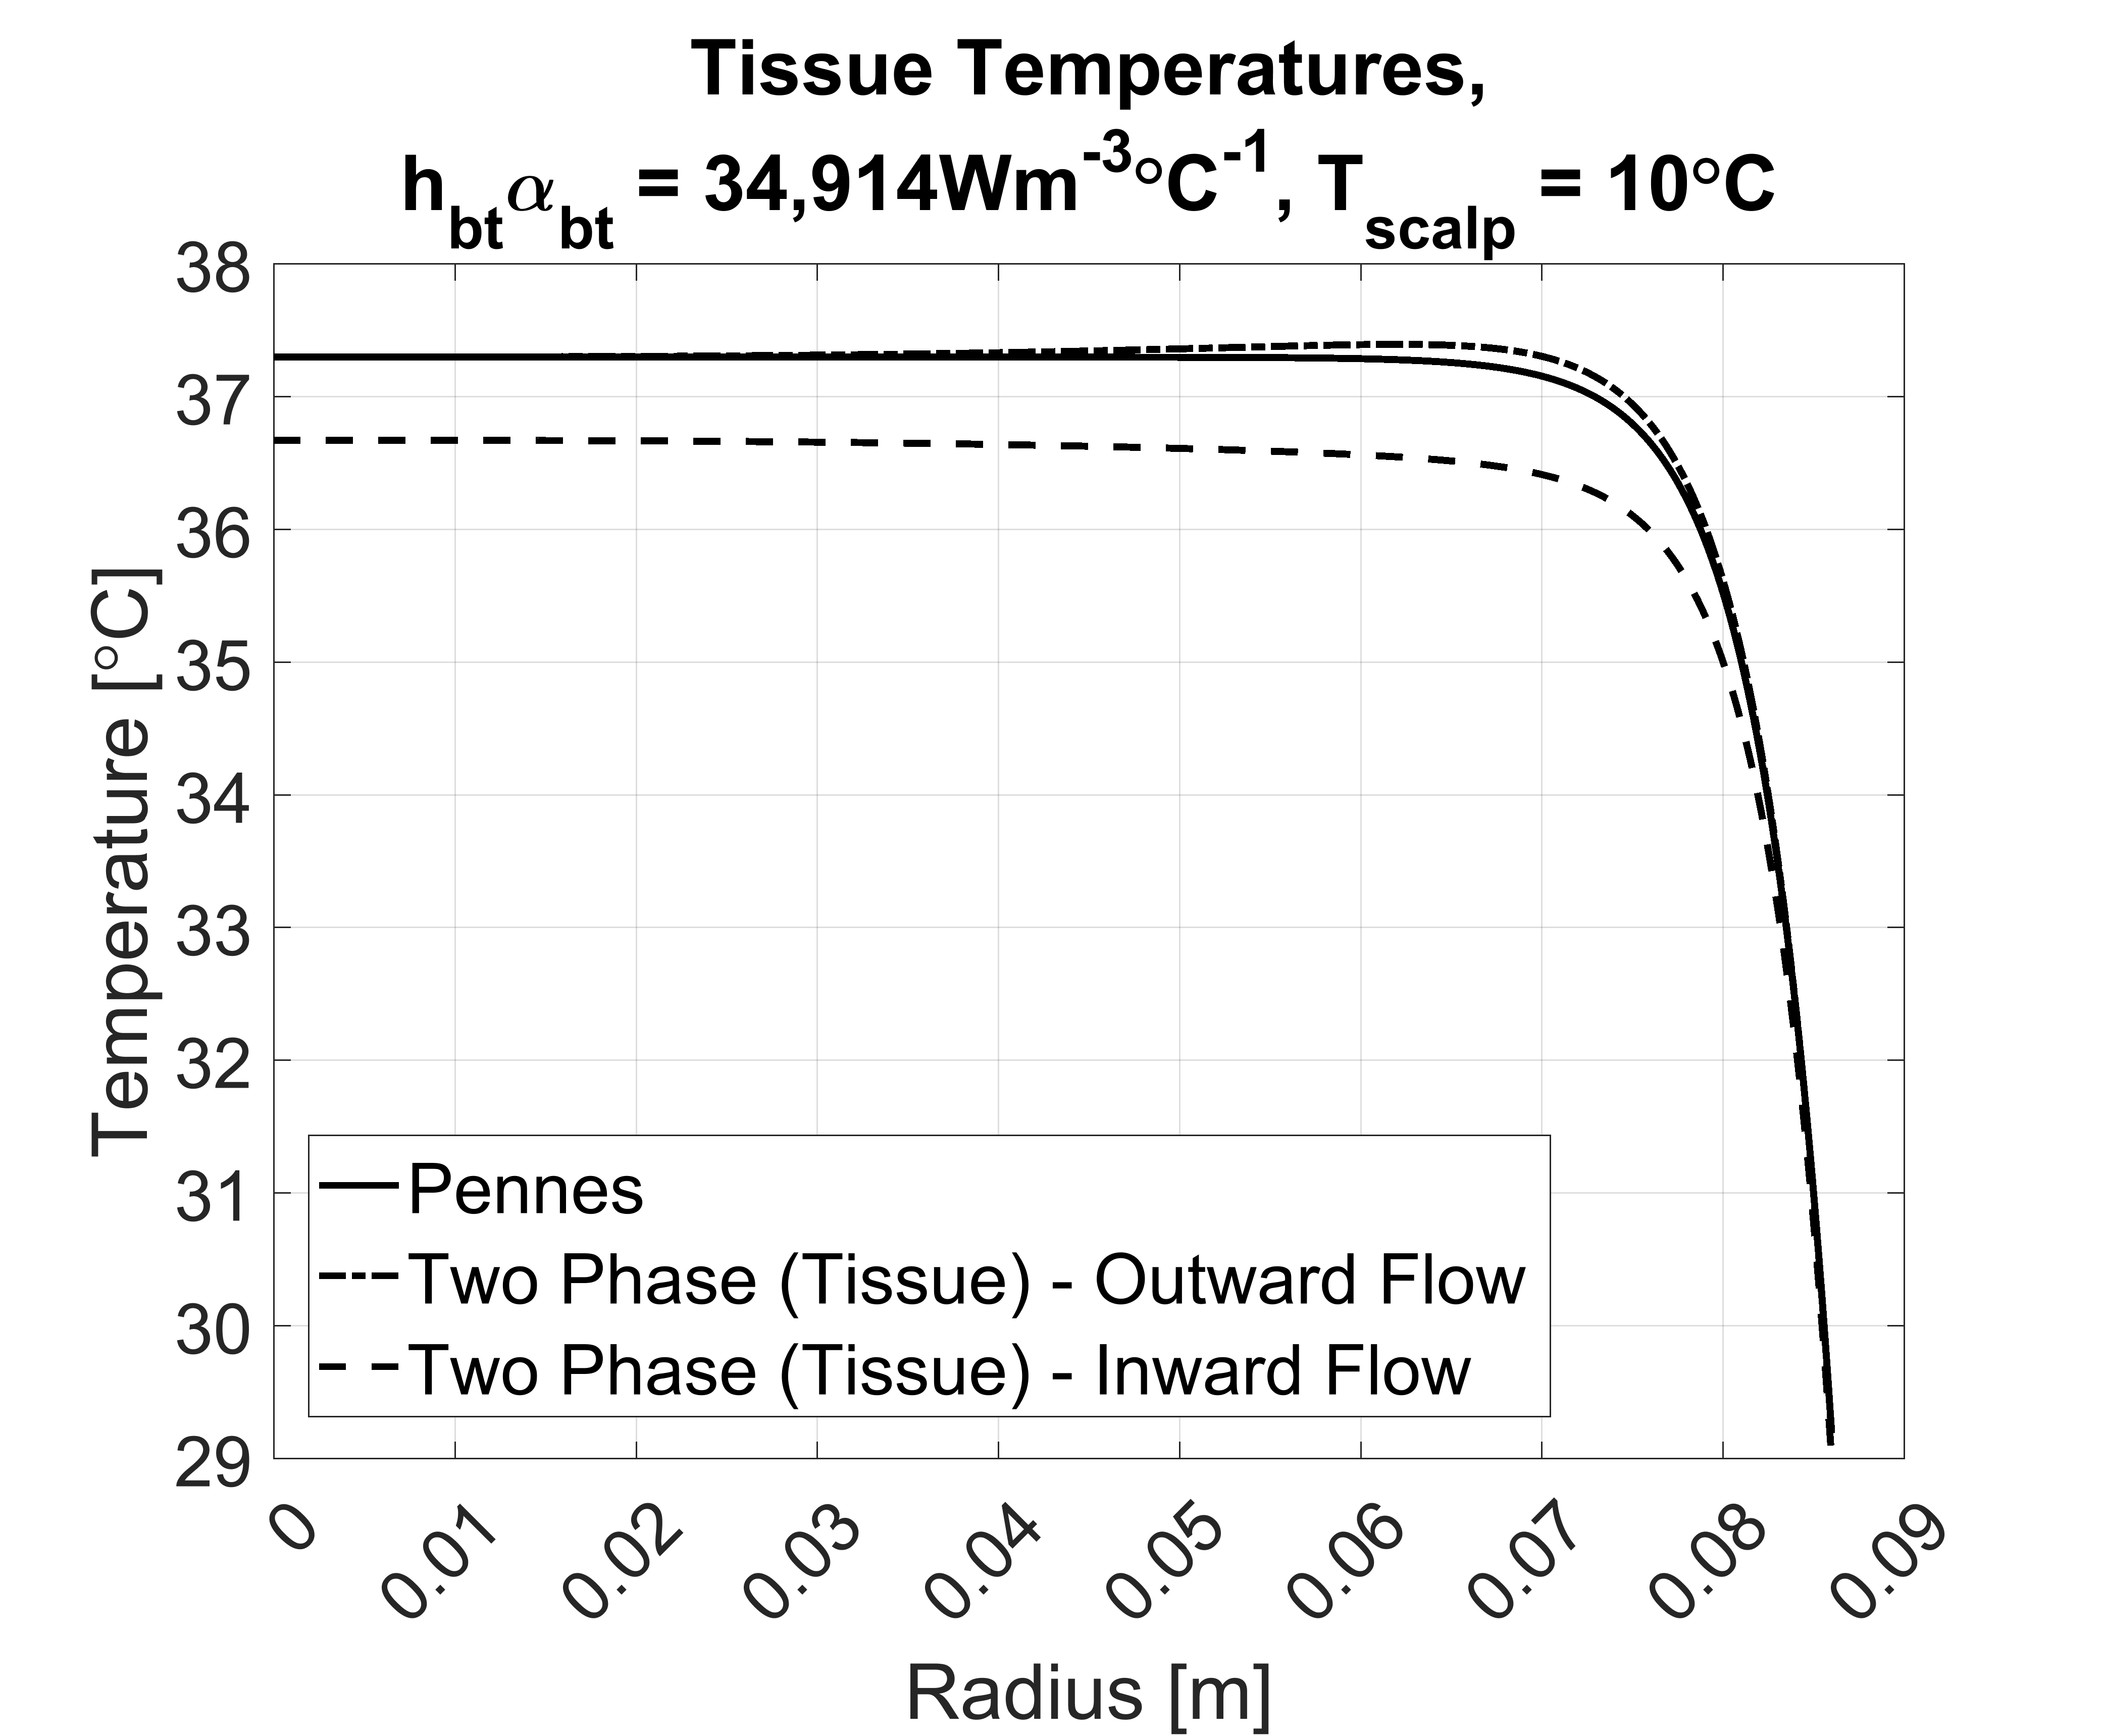
\includegraphics[width=\textwidth]{1DHemisphere/figure4}
	\end{subfigure}
	\caption[Radial temperature distributions for the Pennes Bioheat Equation and Porous Two Phase unidirectional models with $h_{bt}\alpha_{bt} = \text{34,914}W/m^{3}/^{o}C$ for $T_{scalp}=36.5^{o}C$ and $T_{scalp}=10^{o}C$]{Radial temperature distributions for the Pennes Bioheat Equation and Porous Two Phase unidirectional models with $h_{bt}\alpha_{bt} = \text{34,914}W/m^{3}/^{o}C$ for $T_{scalp}=36.5^{o}C$ (left) and $T_{scalp}=10^{o}C$ (right).}
	\label{fig:Results2}
\end{figure}

Figure~\ref{fig:Results2} shows the radial temperature profiles for the Pennes Bioheat Equations and Porous Two Phase model at $h_{bt}\alpha_{bt} = \text{34,914}W/m^{3}/^{o}C$ under normal and cooling conditions. The average temperatures for the Two Phase model with this inter-phase heat transfer are higher than Pennes at normal scalp temperature ($37.41^{o}C$ and $37.39^{o}C$ for outward and inward flow directions respectively). This is due to the imposed temperature driving force required for blood and tissue transfer. This effectively doubles the expected rise of tissue temperature to $0.6^{o}C$. The temperature profiles are similar in shape to the corresponding outward and inward flow profiles in the Wulff/Klinger model in Figure~\ref{fig:Results1} however, they exist over a larger temperature range.

\begin{figure}[h]
	\centering
	\begin{subfigure}[b]{0.49\textwidth}
		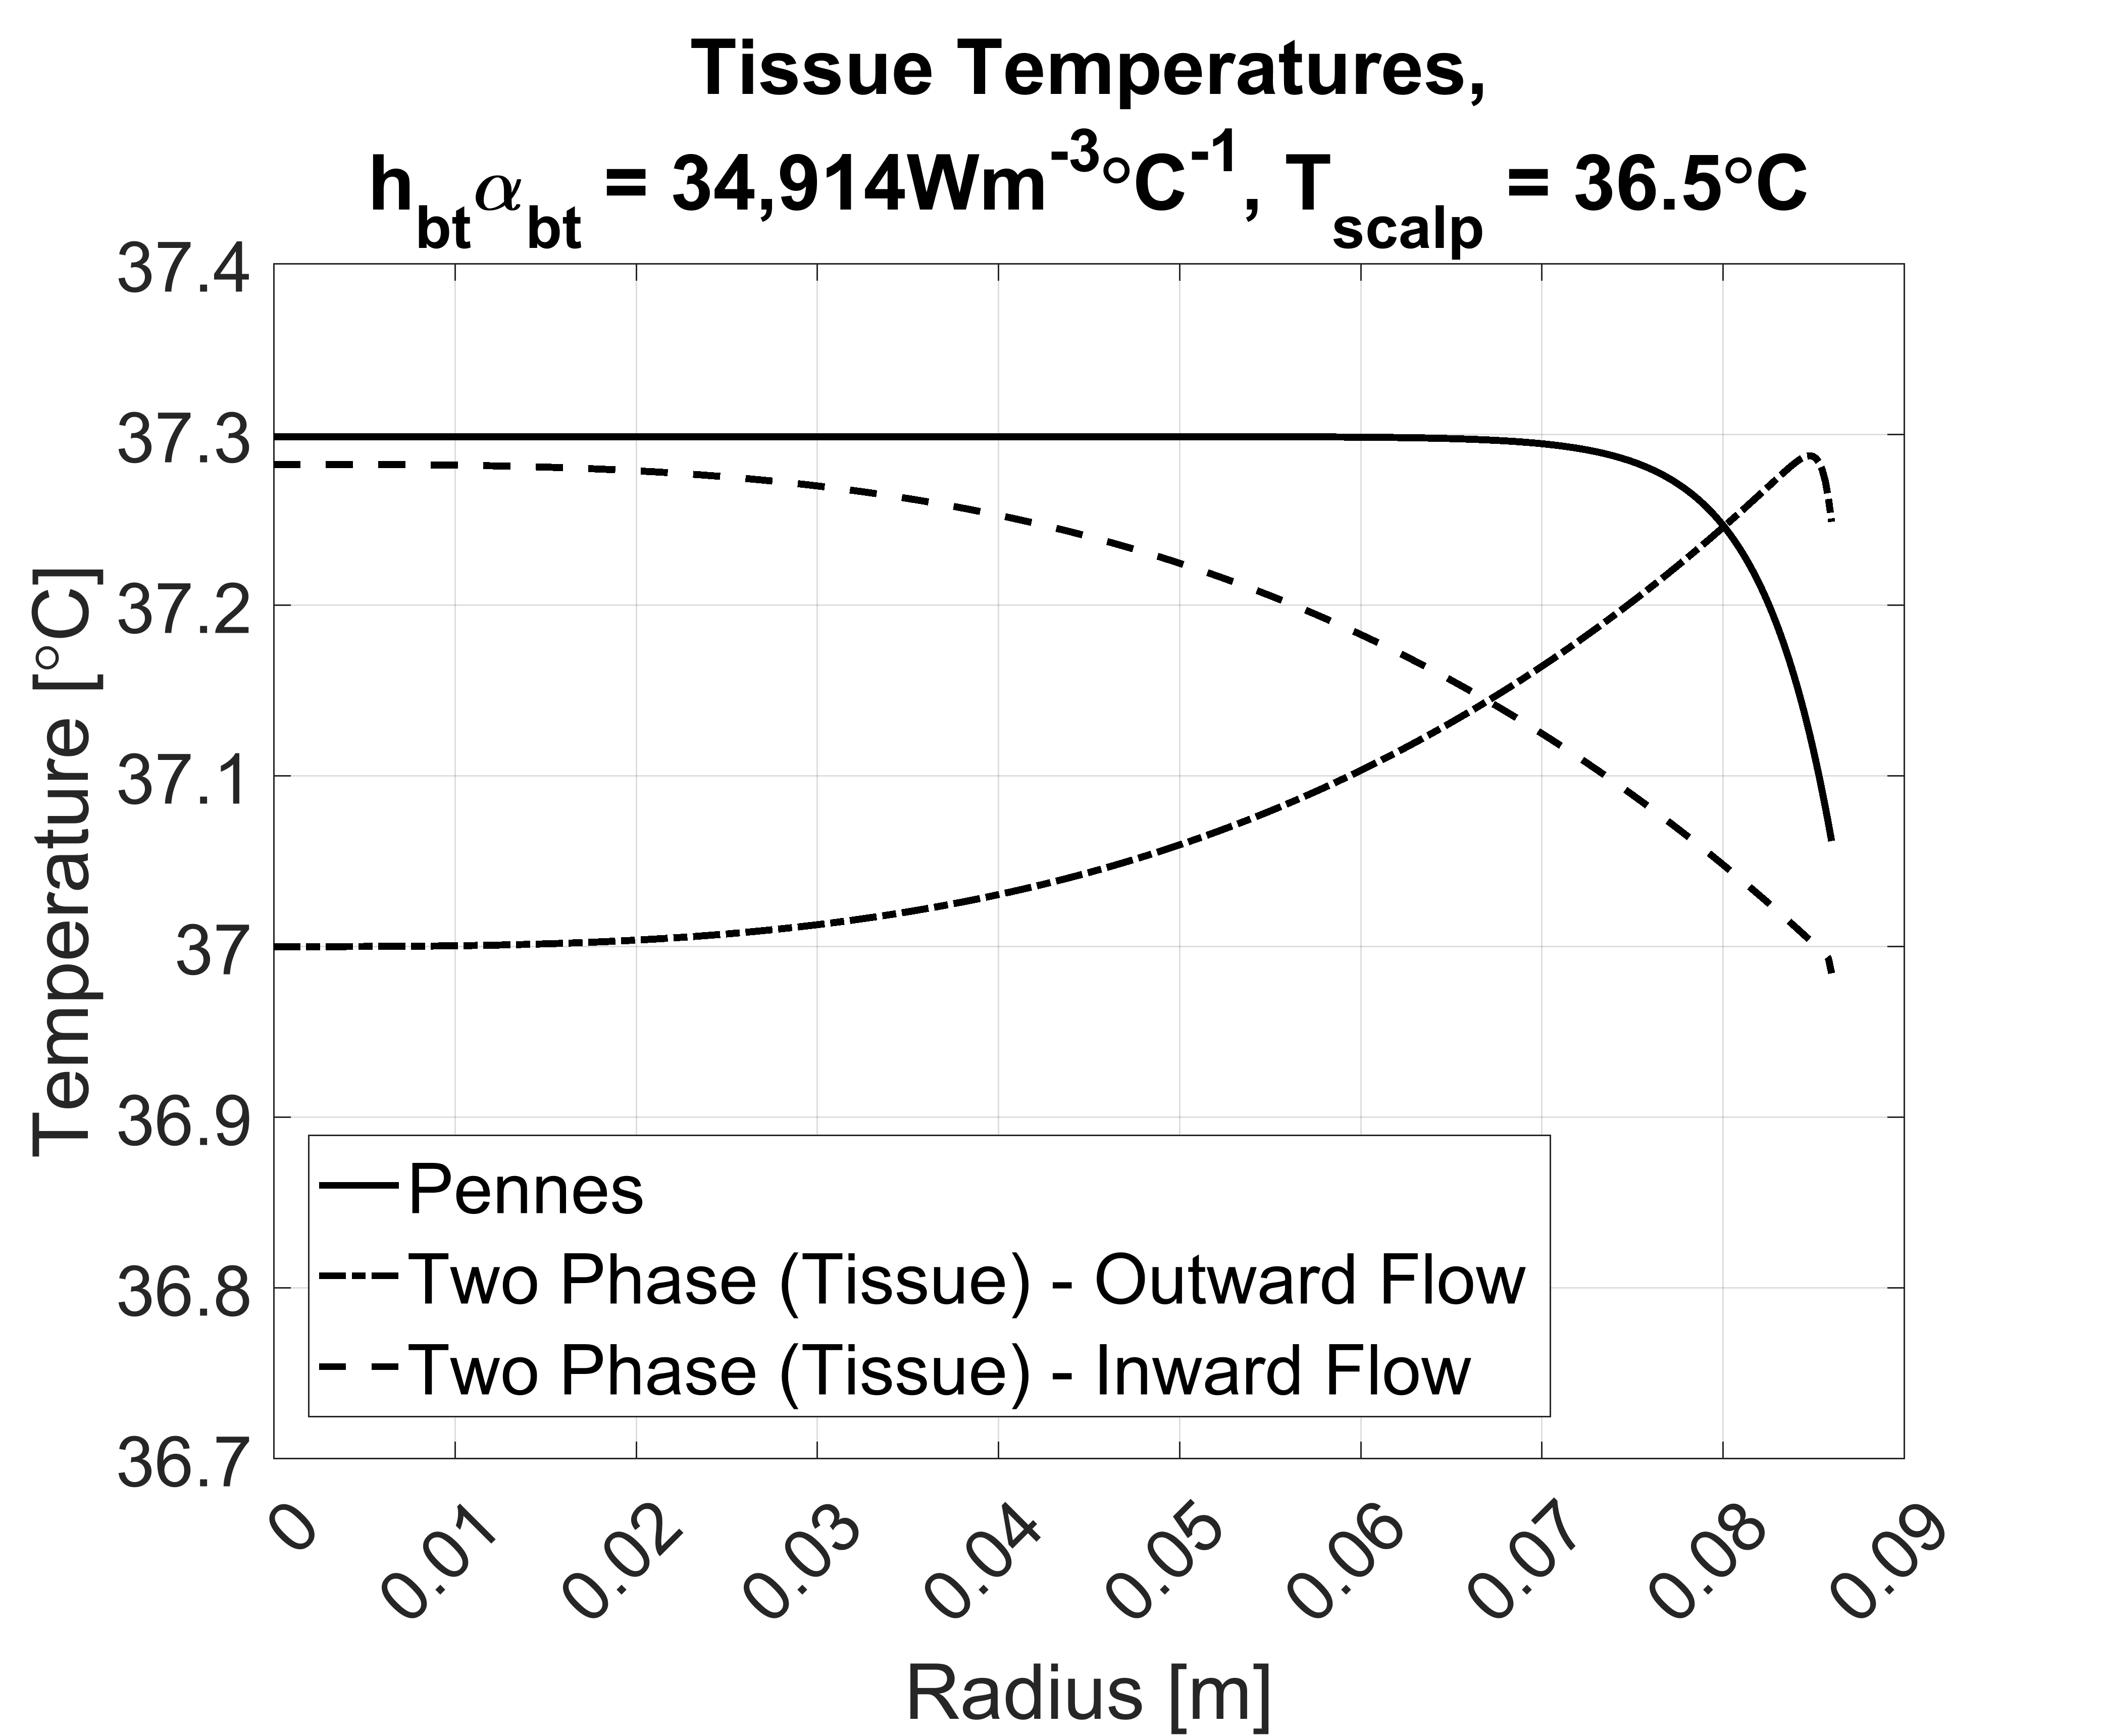
\includegraphics[width=\textwidth]{1DHemisphere/figure5}
	\end{subfigure}
	\begin{subfigure}[b]{0.49\textwidth}
		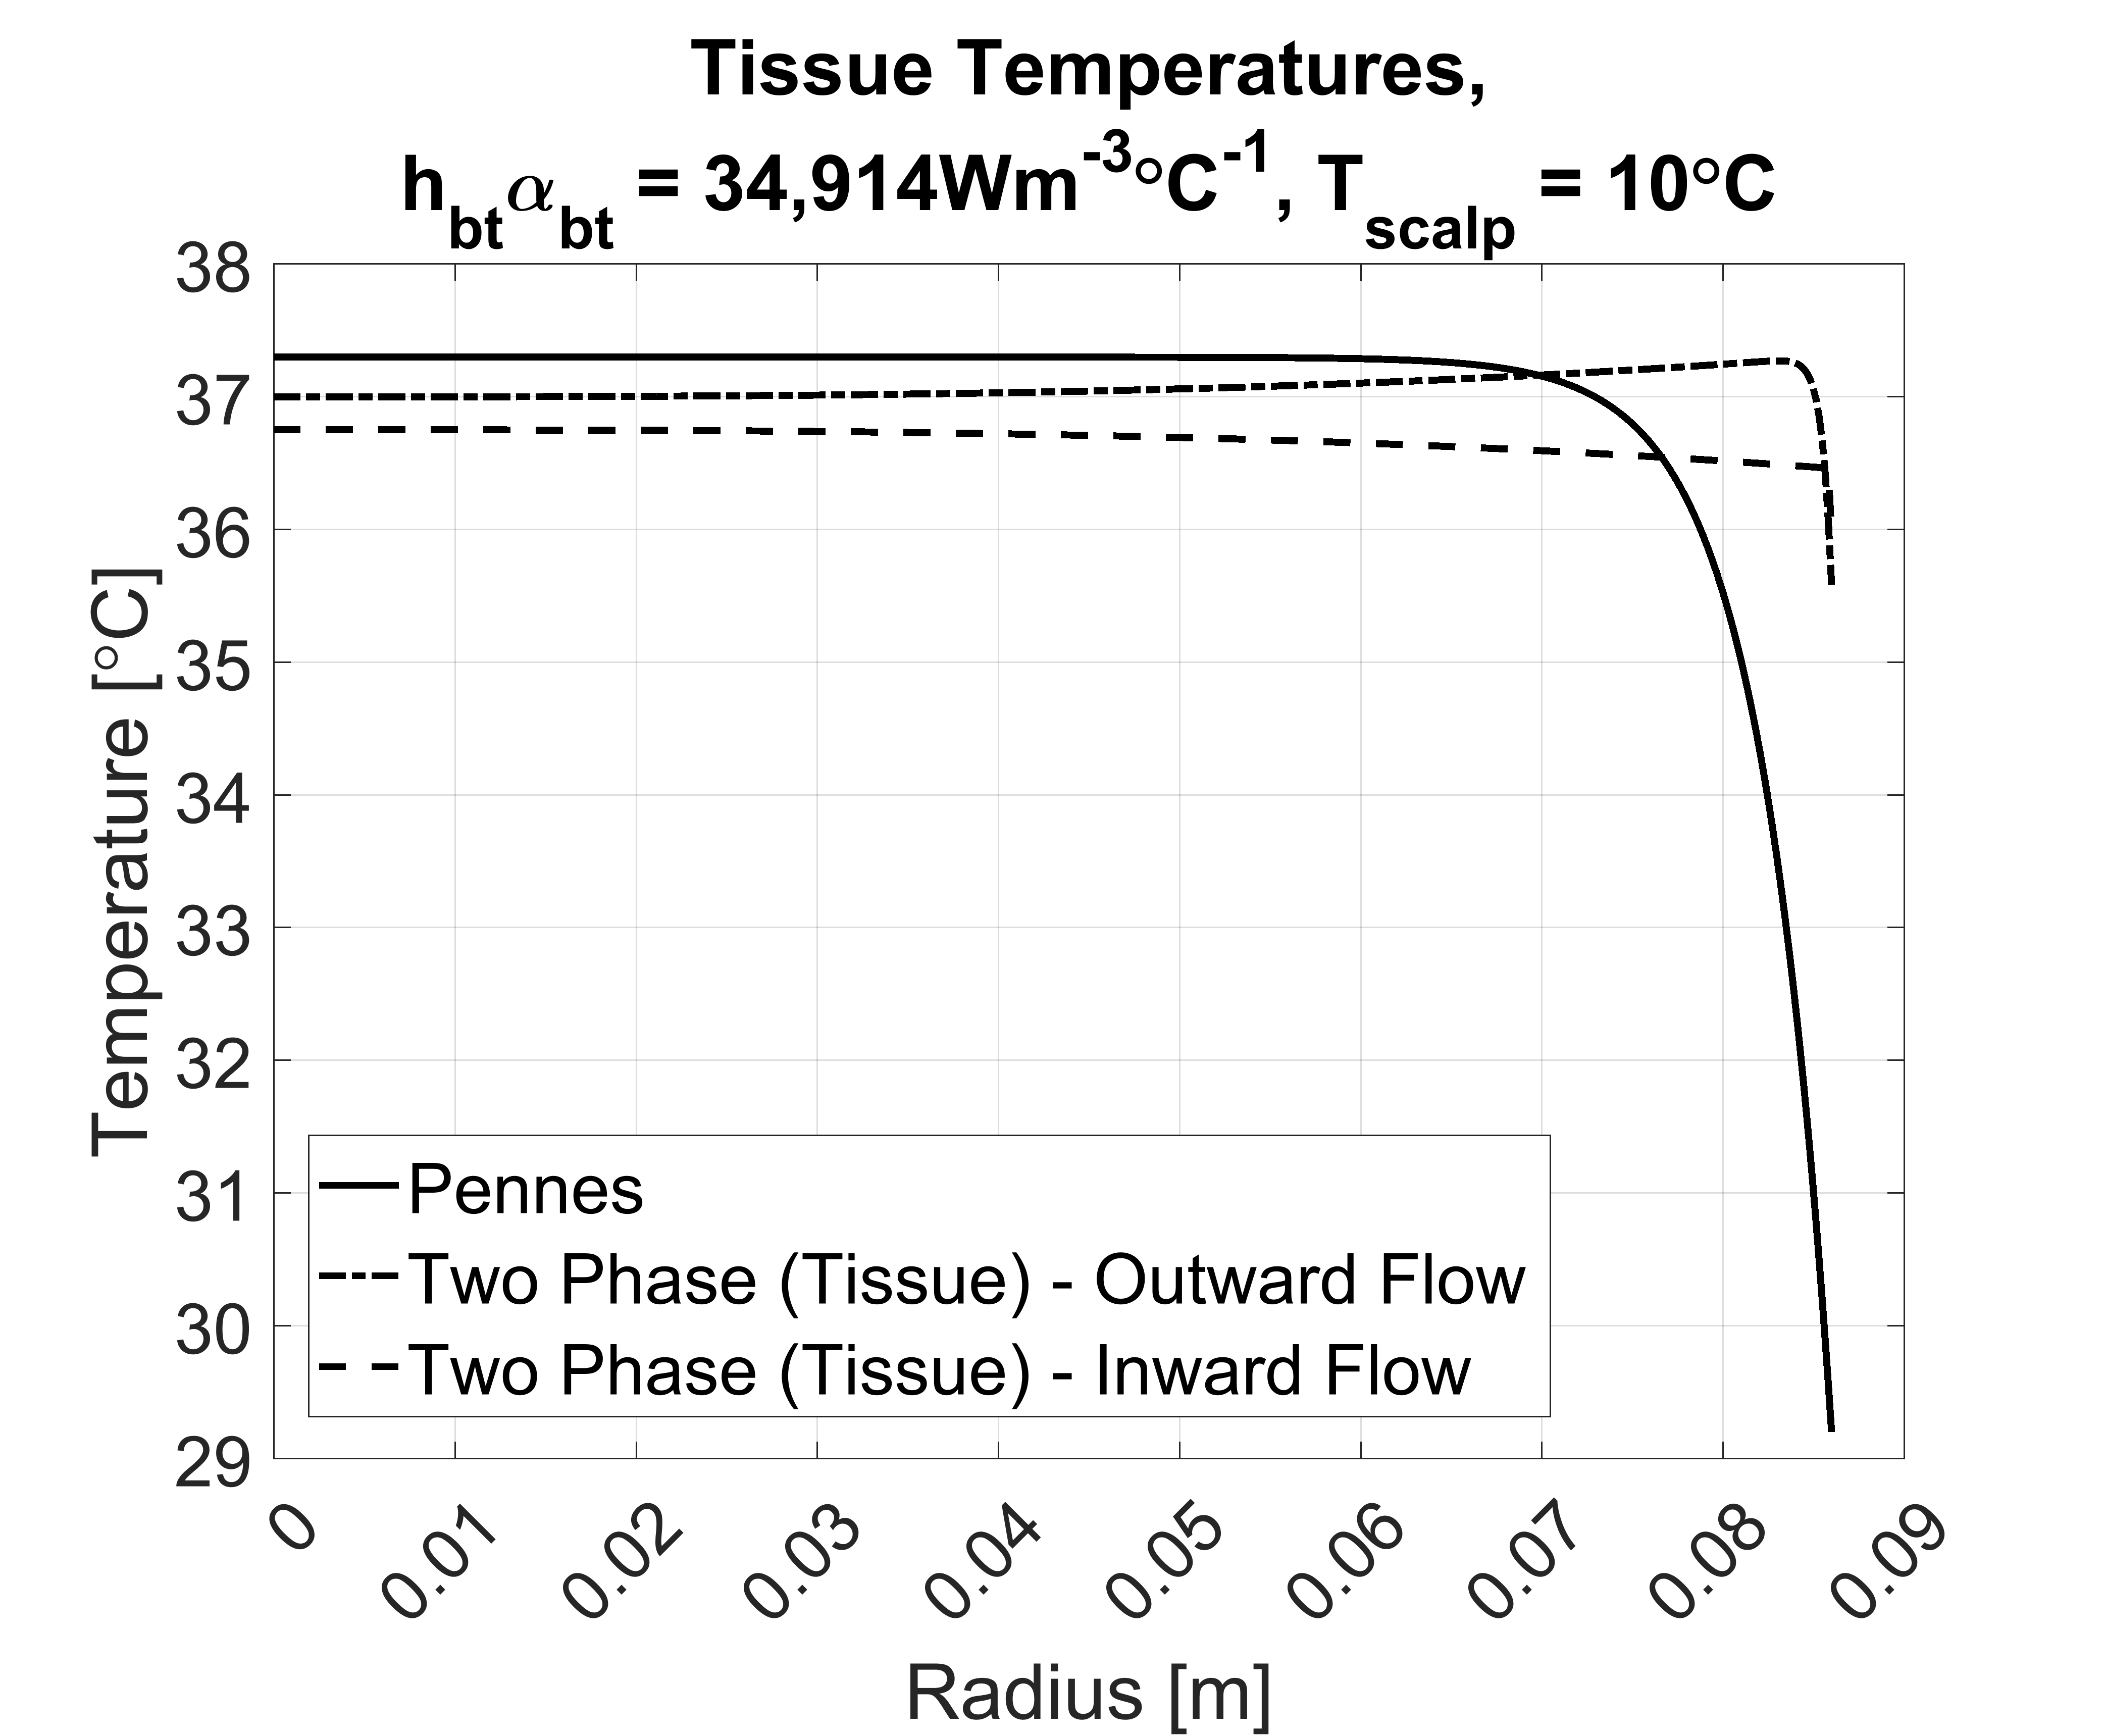
\includegraphics[width=\textwidth]{1DHemisphere/figure6}
	\end{subfigure}
	\caption[Radial temperature distributions for the Pennes Bioheat Equation and Porous Two Phase unidirectional models with $h_{bt}\alpha_{bt} = 10^{8}W/m^{3}/^{o}C$ for $T_{scalp}=36.5^{o}C$ and $T_{scalp}=10^{o}C$]{Radial temperature distributions for the Pennes Bioheat Equation and Porous Two Phase unidirectional models with $h_{bt}\alpha_{bt} = 10^{8}W/m^{3}/^{o}C$ for $T_{scalp}=36.5^{o}C$ (left) and $T_{scalp}=10^{o}C$ (right).}
	\label{fig:Results3}
\end{figure}

Figure~\ref{fig:Results3} shows the radial temperature profiles for the Pennes Bioheat Equations and Porous Two Phase model at $h_{bt}\alpha_{bt} = 10^{8}W/m^{3}/^{o}C$ under normal and cooling conditions. As expected, the temperature profiles produced here are almost identical to the temperature profiles in Figure~\ref{fig:Results1} for the Wulff/Klinger model. There is a slight discrepancy due to the difference in boundary conditions at the surface. This mainly affects the inward flow model when cooling, which displays an uniform temperature increase of $0.79^{o}C$ throughout the tissue compared to the corresponding Wulff/Klinger model.

\begin{figure}[h]
	\centering
	\begin{subfigure}[b]{0.49\textwidth}
		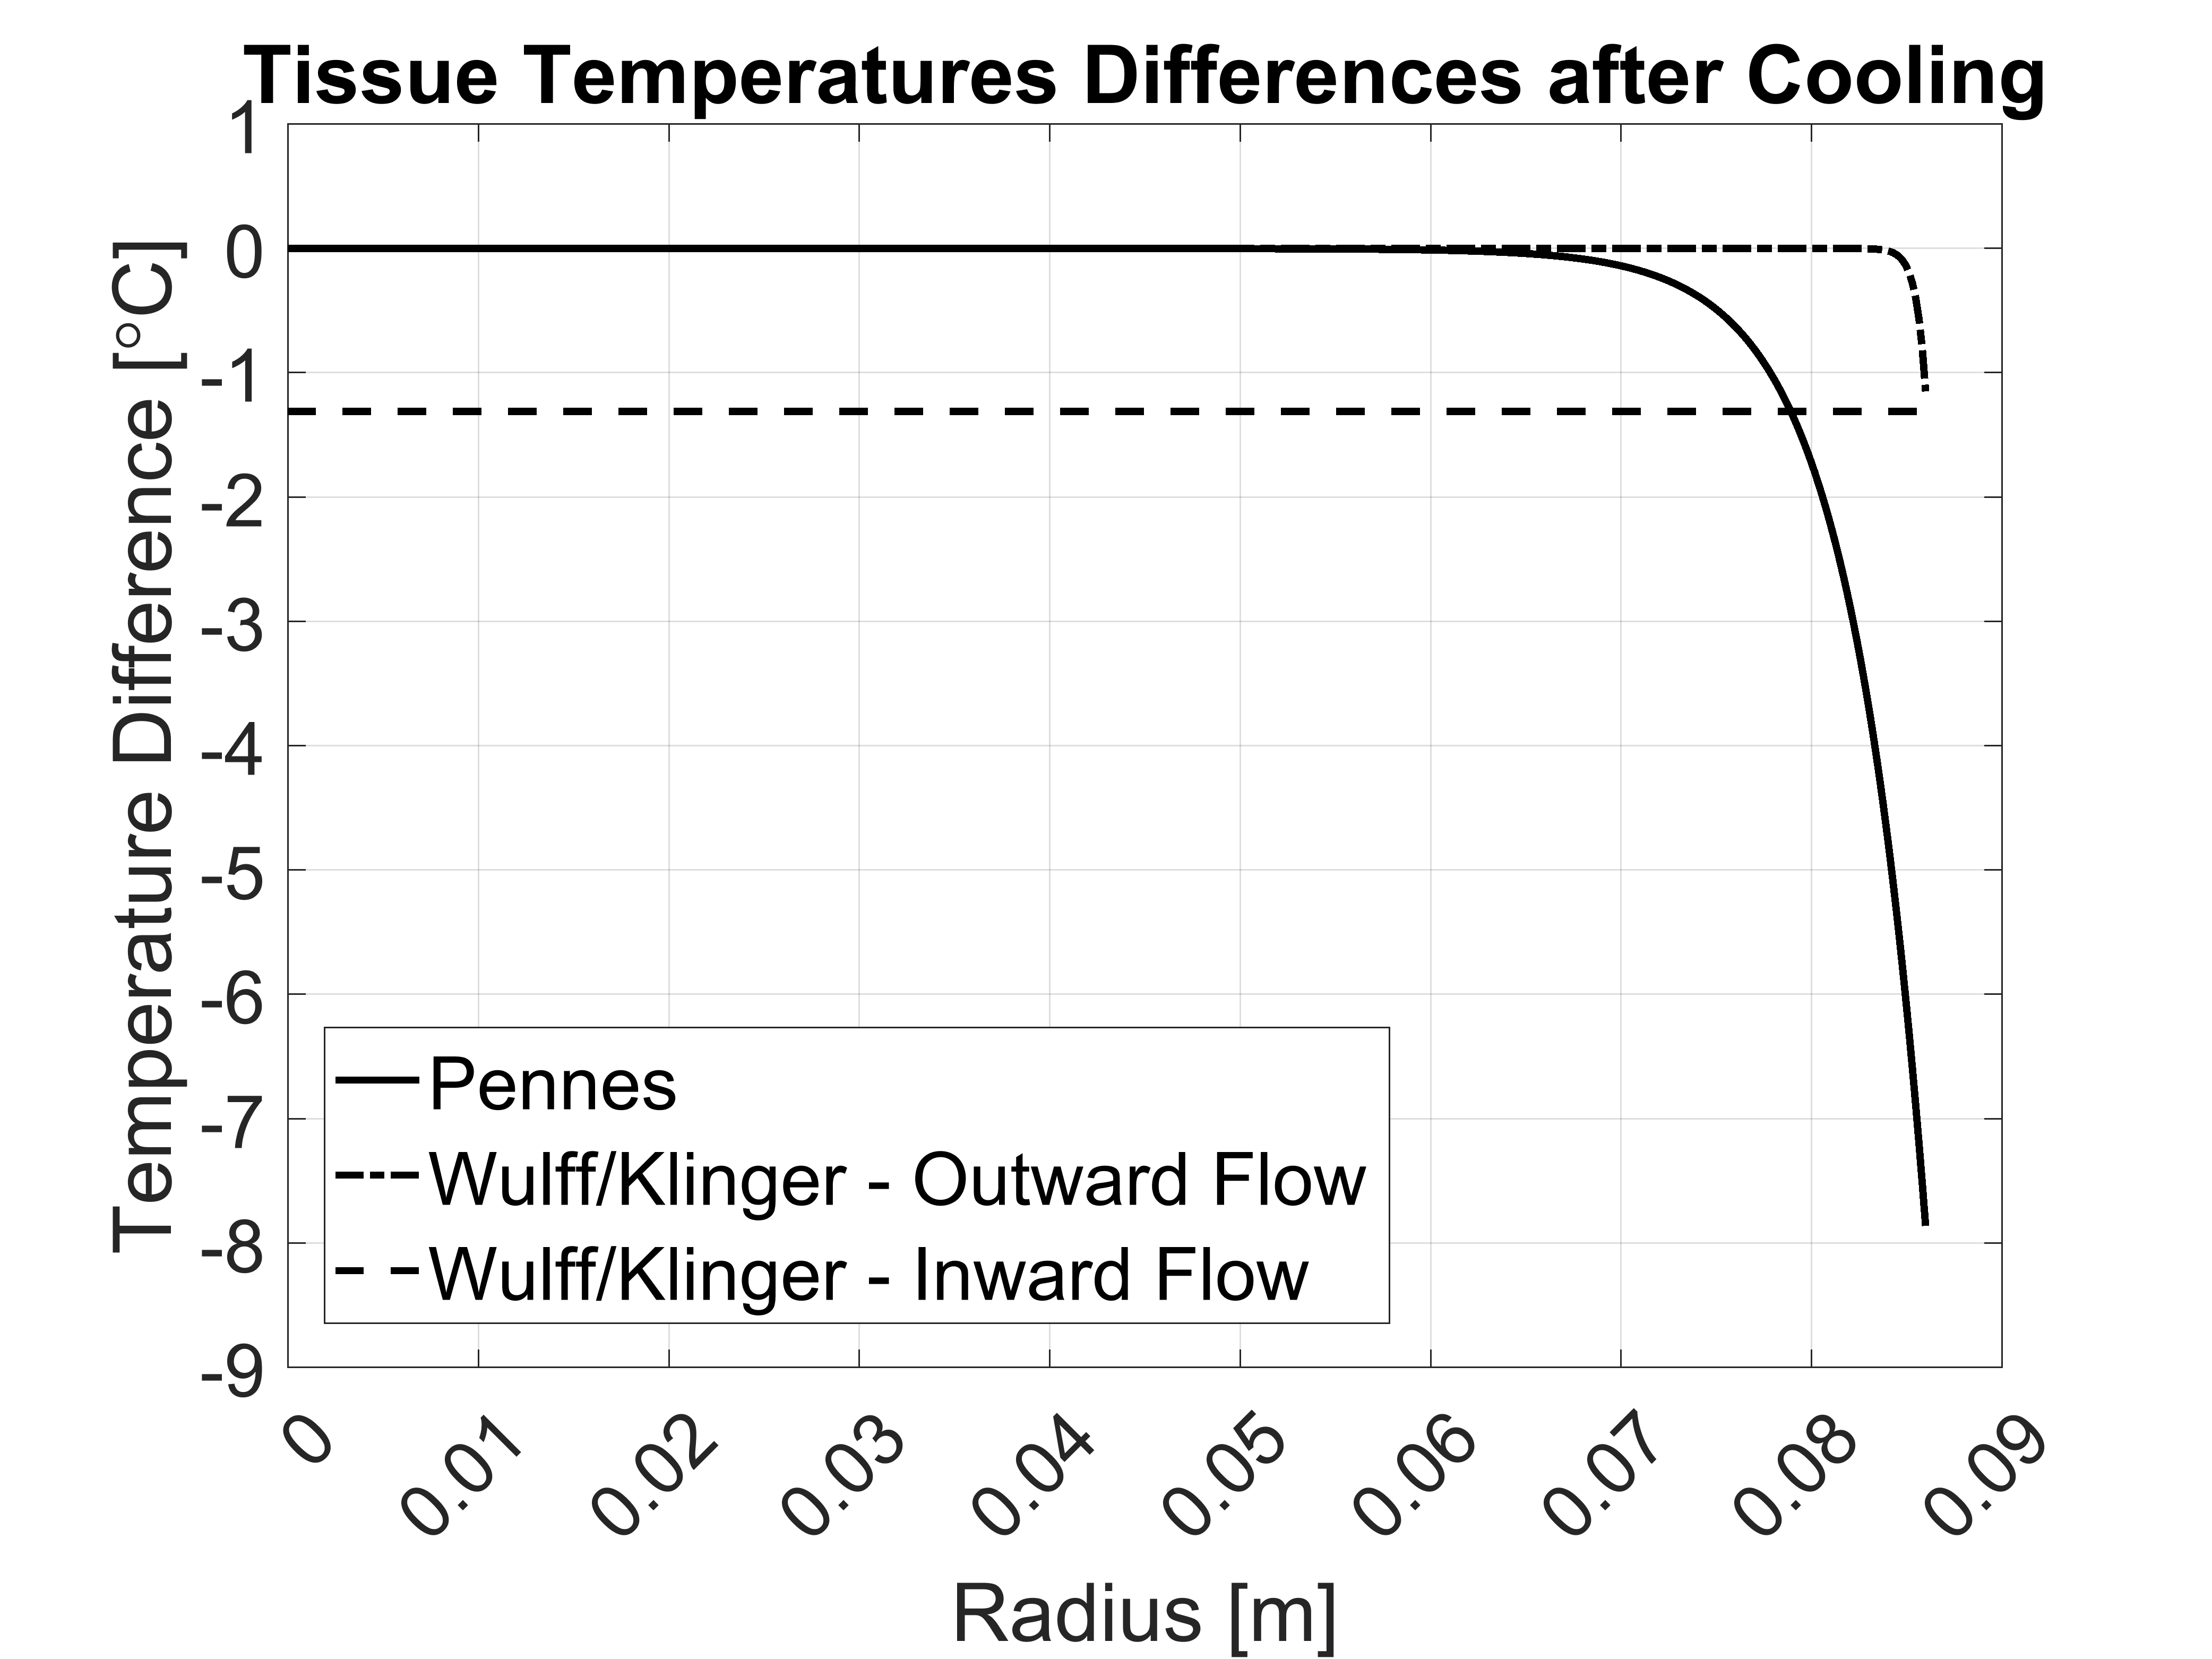
\includegraphics[width=\textwidth]{1DHemisphere/figure7}
	\end{subfigure}
	
	\begin{subfigure}[b]{0.49\textwidth}
		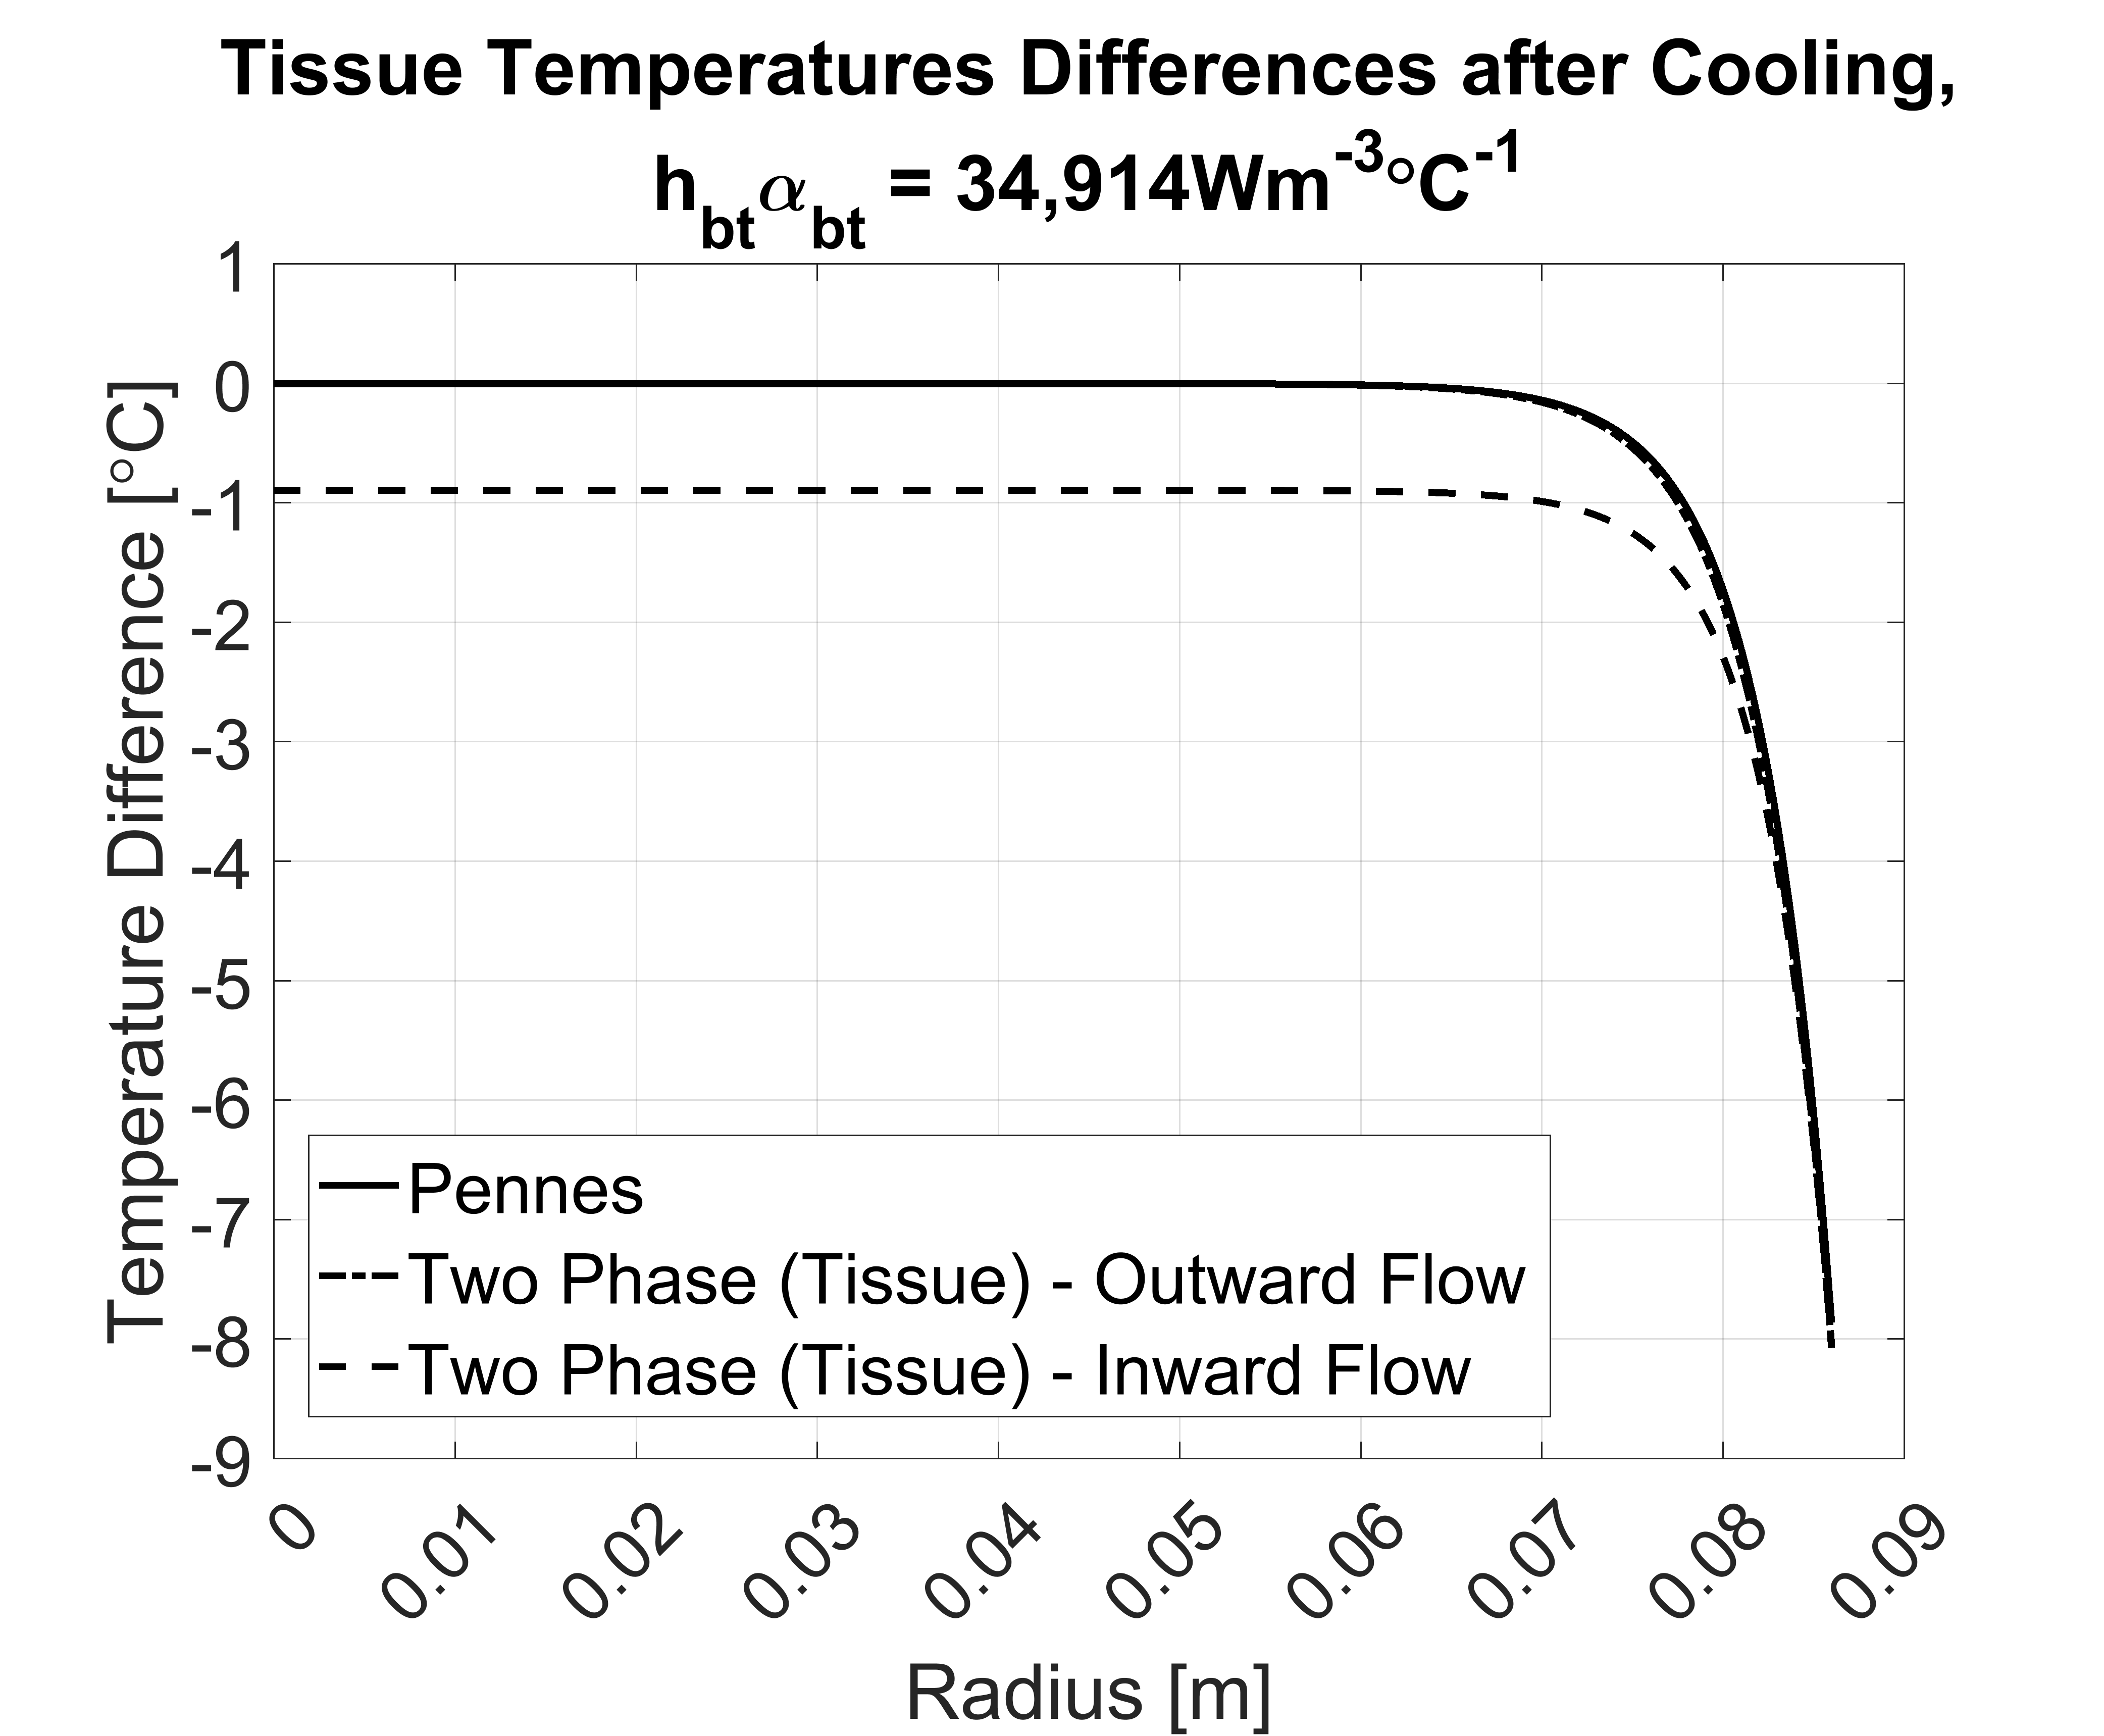
\includegraphics[width=\textwidth]{1DHemisphere/figure8}
	\end{subfigure}
	\begin{subfigure}[b]{0.49\textwidth}
		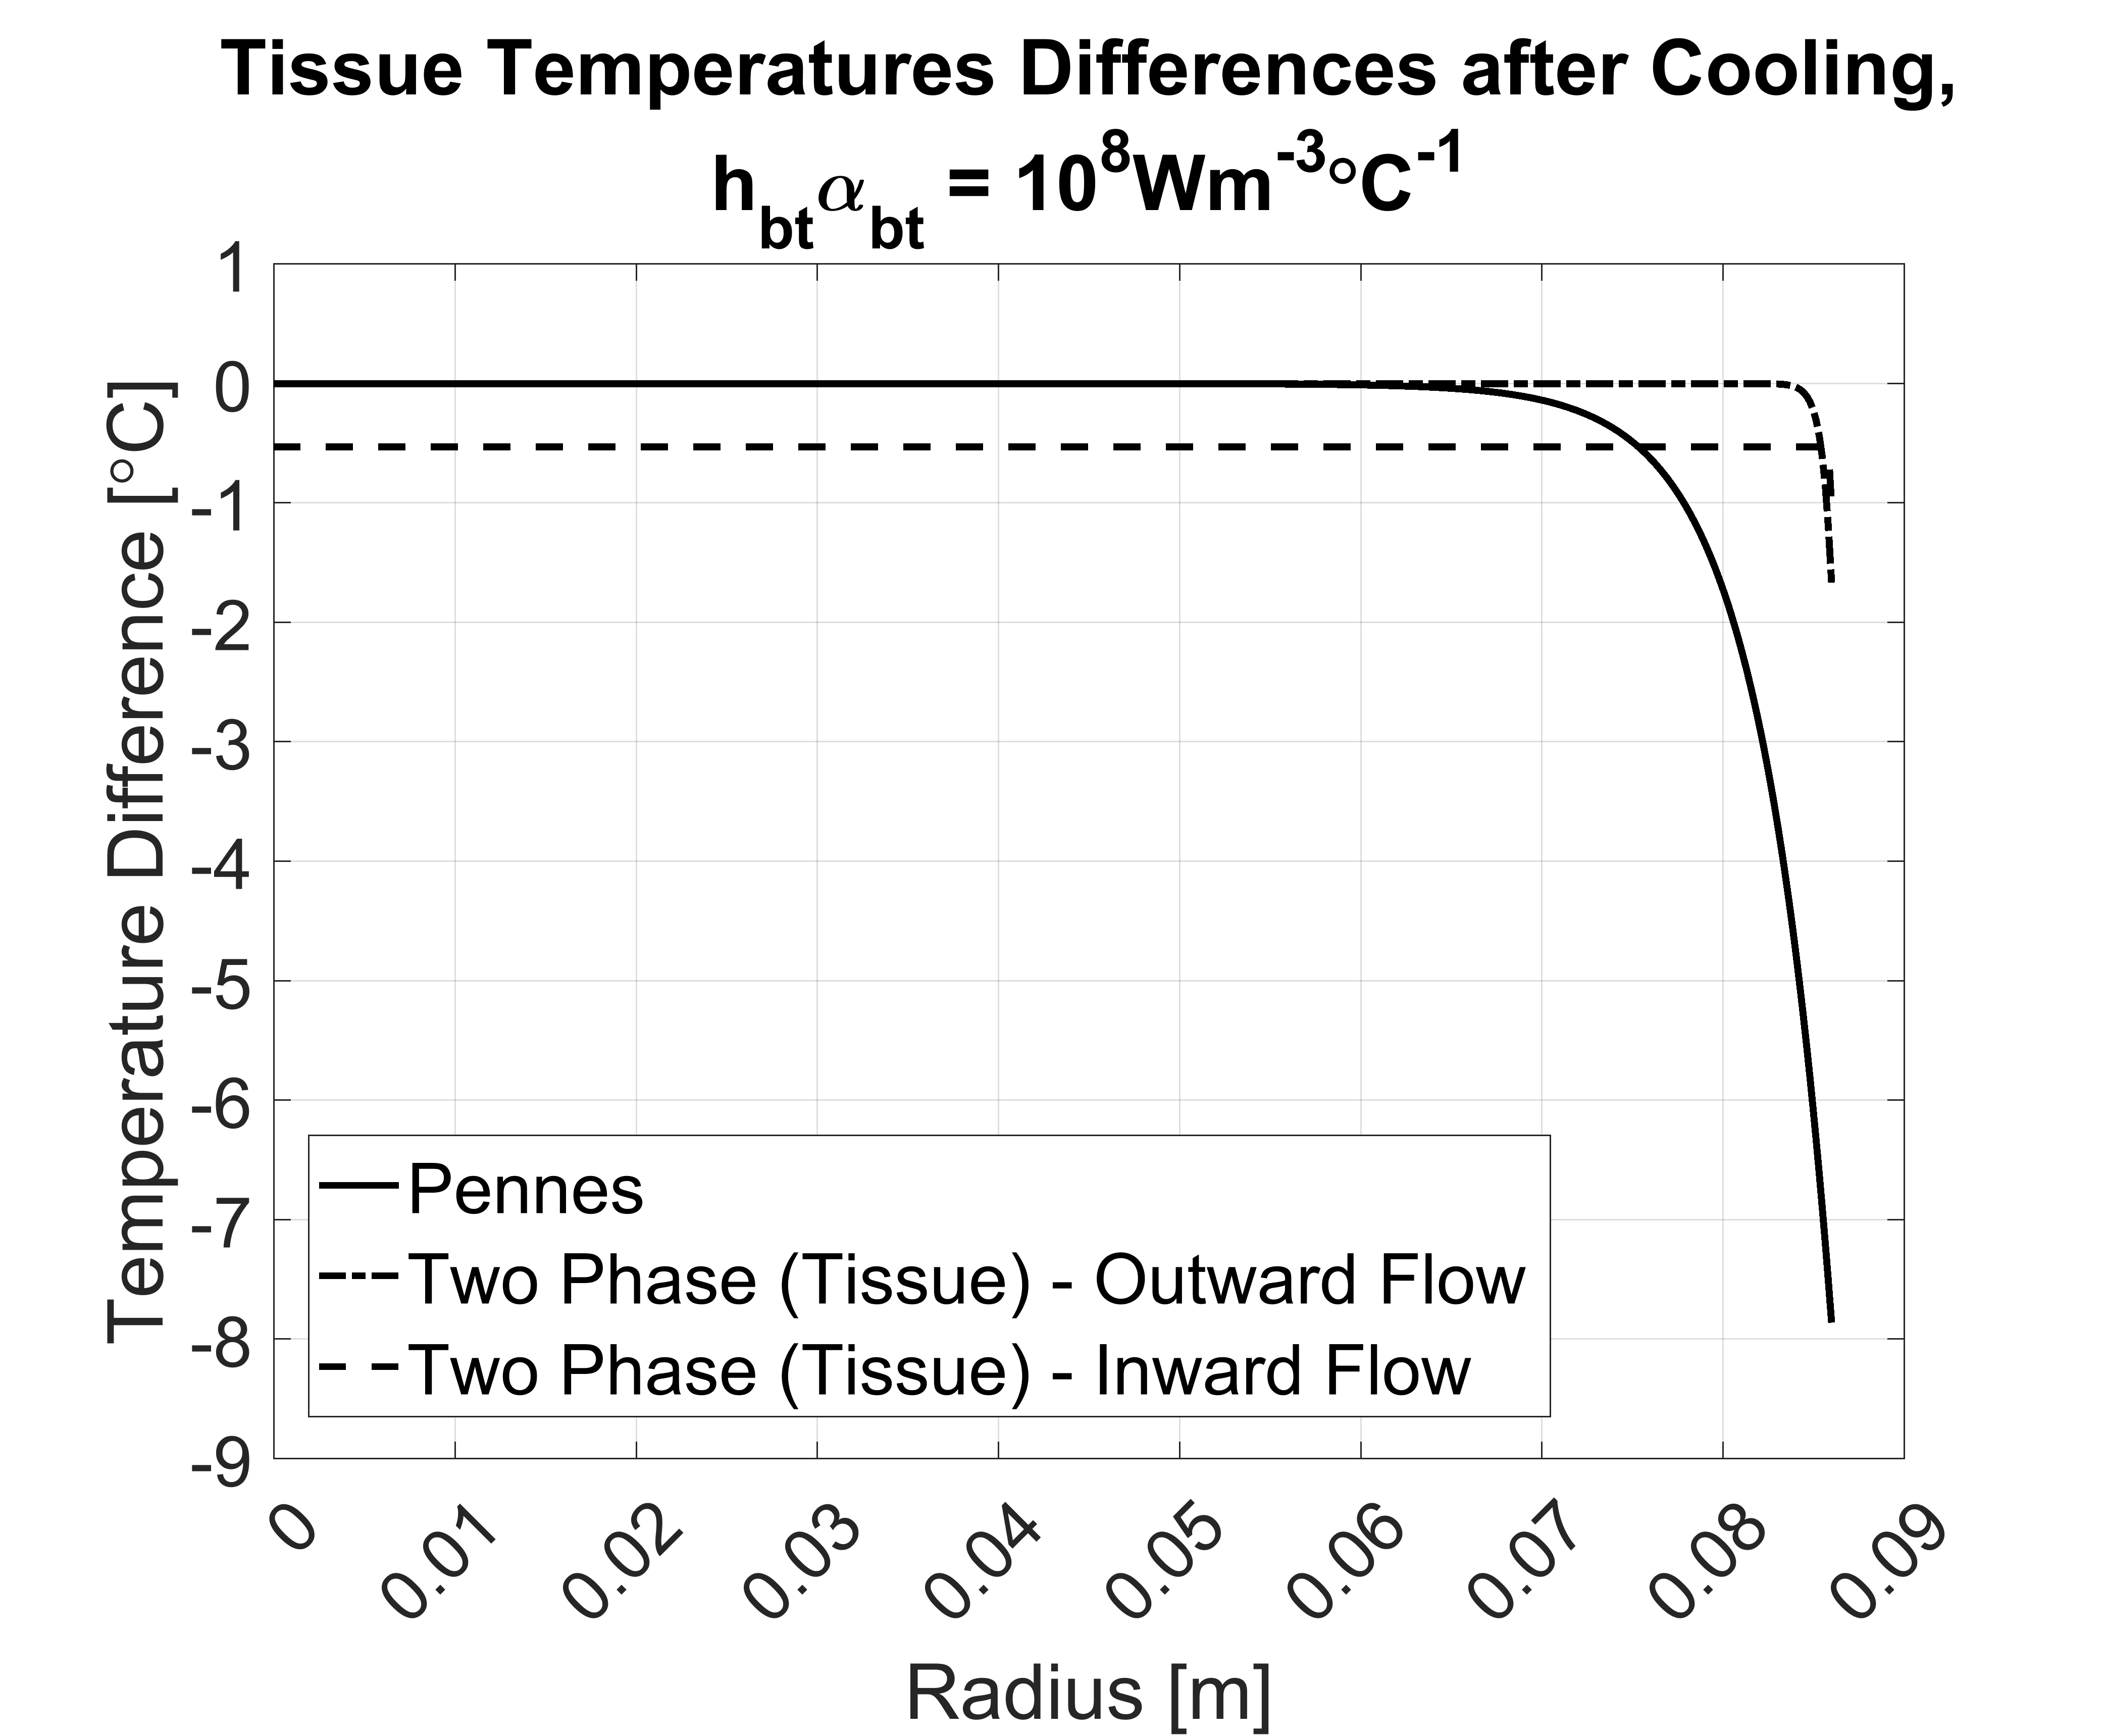
\includegraphics[width=\textwidth]{1DHemisphere/figure9}
	\end{subfigure}
	\caption[Radial profiles of the differences between the temperature profiles at $T_{scalp}=36.5^{o}C$ and $T_{scalp}=10^{o}C$]{Radial profiles of the differences between the temperature profiles at $T_{scalp}=36.5^{o}C$ and $T_{scalp}=10^{o}C$. Each figure is comparing the Pennes Bioheat Equations with the Wulff/Klinger model (top) and Two Phase unidirectional model with $h_{bt}\alpha_{bt} = \text{34,914}W/m^{3}/^{o}C$ (bottom left) and $h_{bt}\alpha_{bt} = 10^{8}W/m^{3}/^{o}C$ (bottom right).}
	\label{fig:Results4}
\end{figure}

Figure~\ref{fig:Results4} shows the temperature differences for all models after cooling. The average temperature drop for the Pennes model was $0.99^{o}C$, however, this is located namely in the outer $1.6cm$ of tissue. Within the bound $r{<}7cm$, the average temperature drop is only $0.02^{o}C$. The average temperature drop for the the Wulff/Klinger model was $0.02^{o}C$ and $1.31^{o}C$ for the outward and inward flow directions respectively. The average temperature drop for the two-phase model at $h_{bt}\alpha_{bt} = \text{34,914}W/m^{3}/^{o}C$ was $1.04^{o}C$ and $1.73^{o}C$ for the outward and inward flow directions respectively. The average temperature drop for the two-phase model at $h_{bt}\alpha_{bt} = 10^{8}W/m^{3}/^{o}C$ was $0.03^{o}C$ and $0.53^{o}C$ for the outward and inward flow directions respectively.

Here, the temperature shielding effect within Pennes Bioheat Equation can be observed as the core temperature remains unaffected from a decrease in surface temperature. This is also observed in all the outward flowing models where the temperature is almost uniformly unaffected except for a small portion of tissue at the surface. The most notable effect is within the inward flow models which all display a uniform cooling throughout the brain. 

\begin{figure}[h]
	\centering
	\begin{subfigure}[b]{0.49\textwidth}
		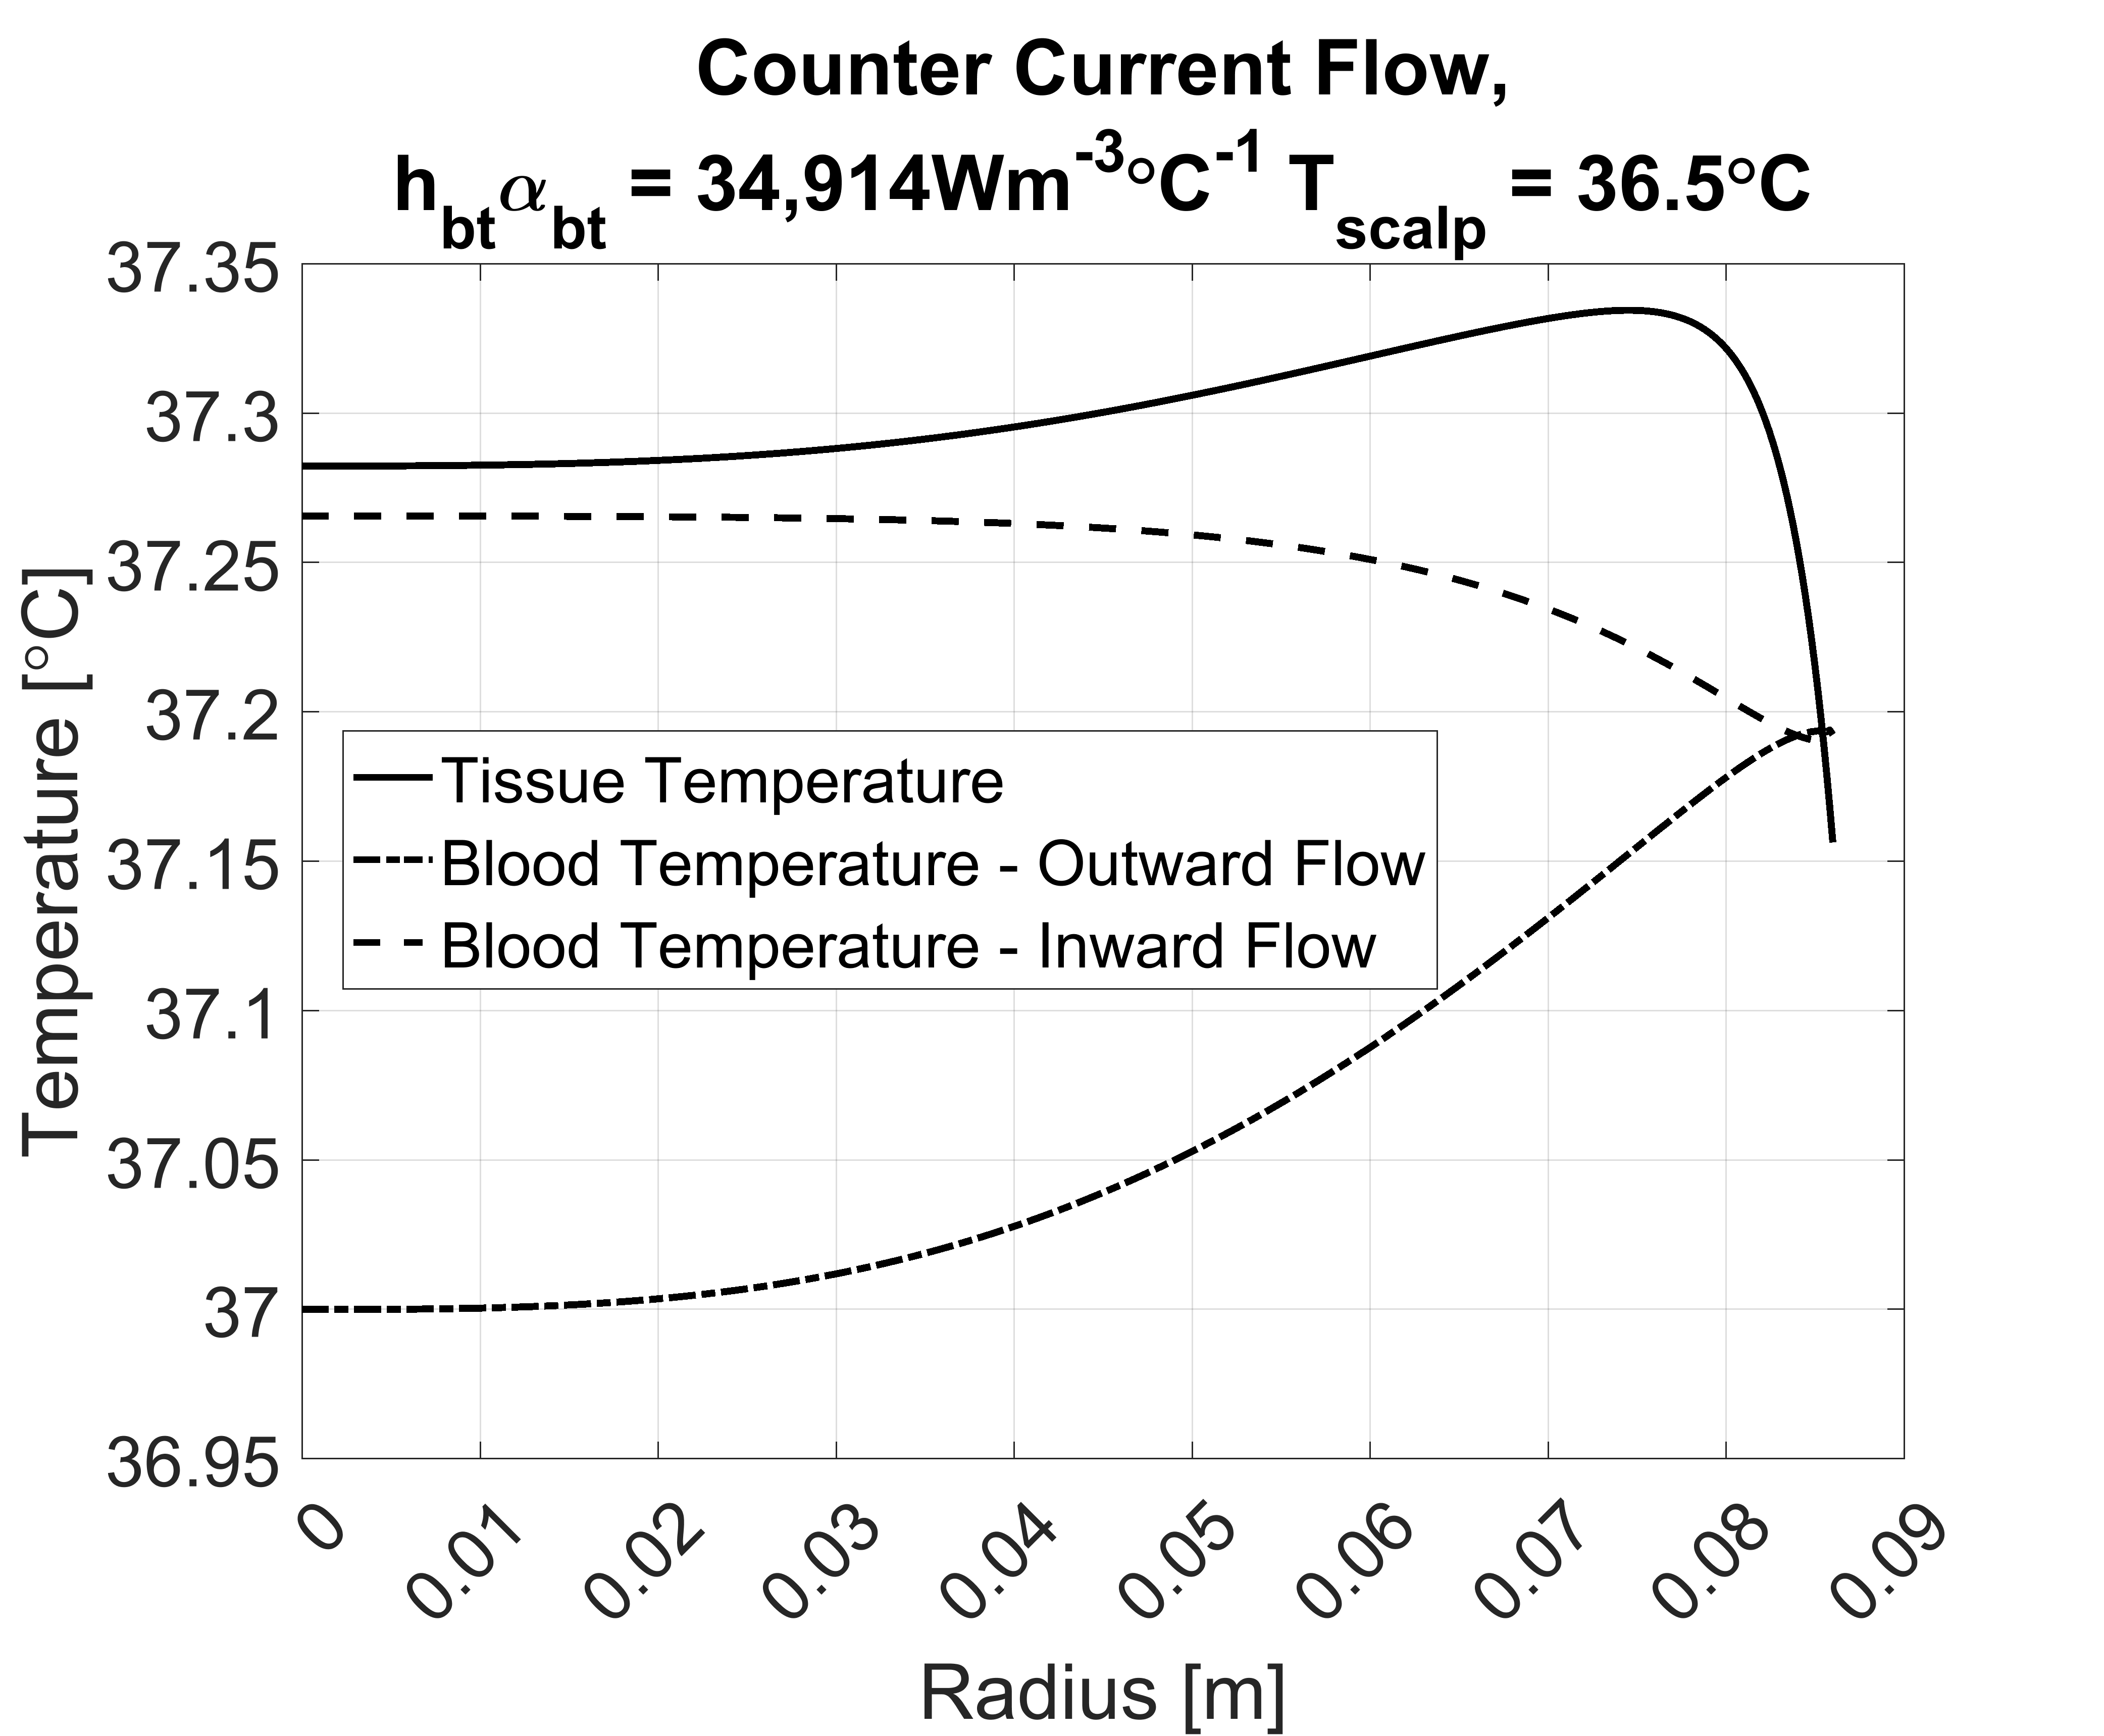
\includegraphics[width=\textwidth]{1DHemisphere/figure10}
	\end{subfigure}
	\begin{subfigure}[b]{0.49\textwidth}
		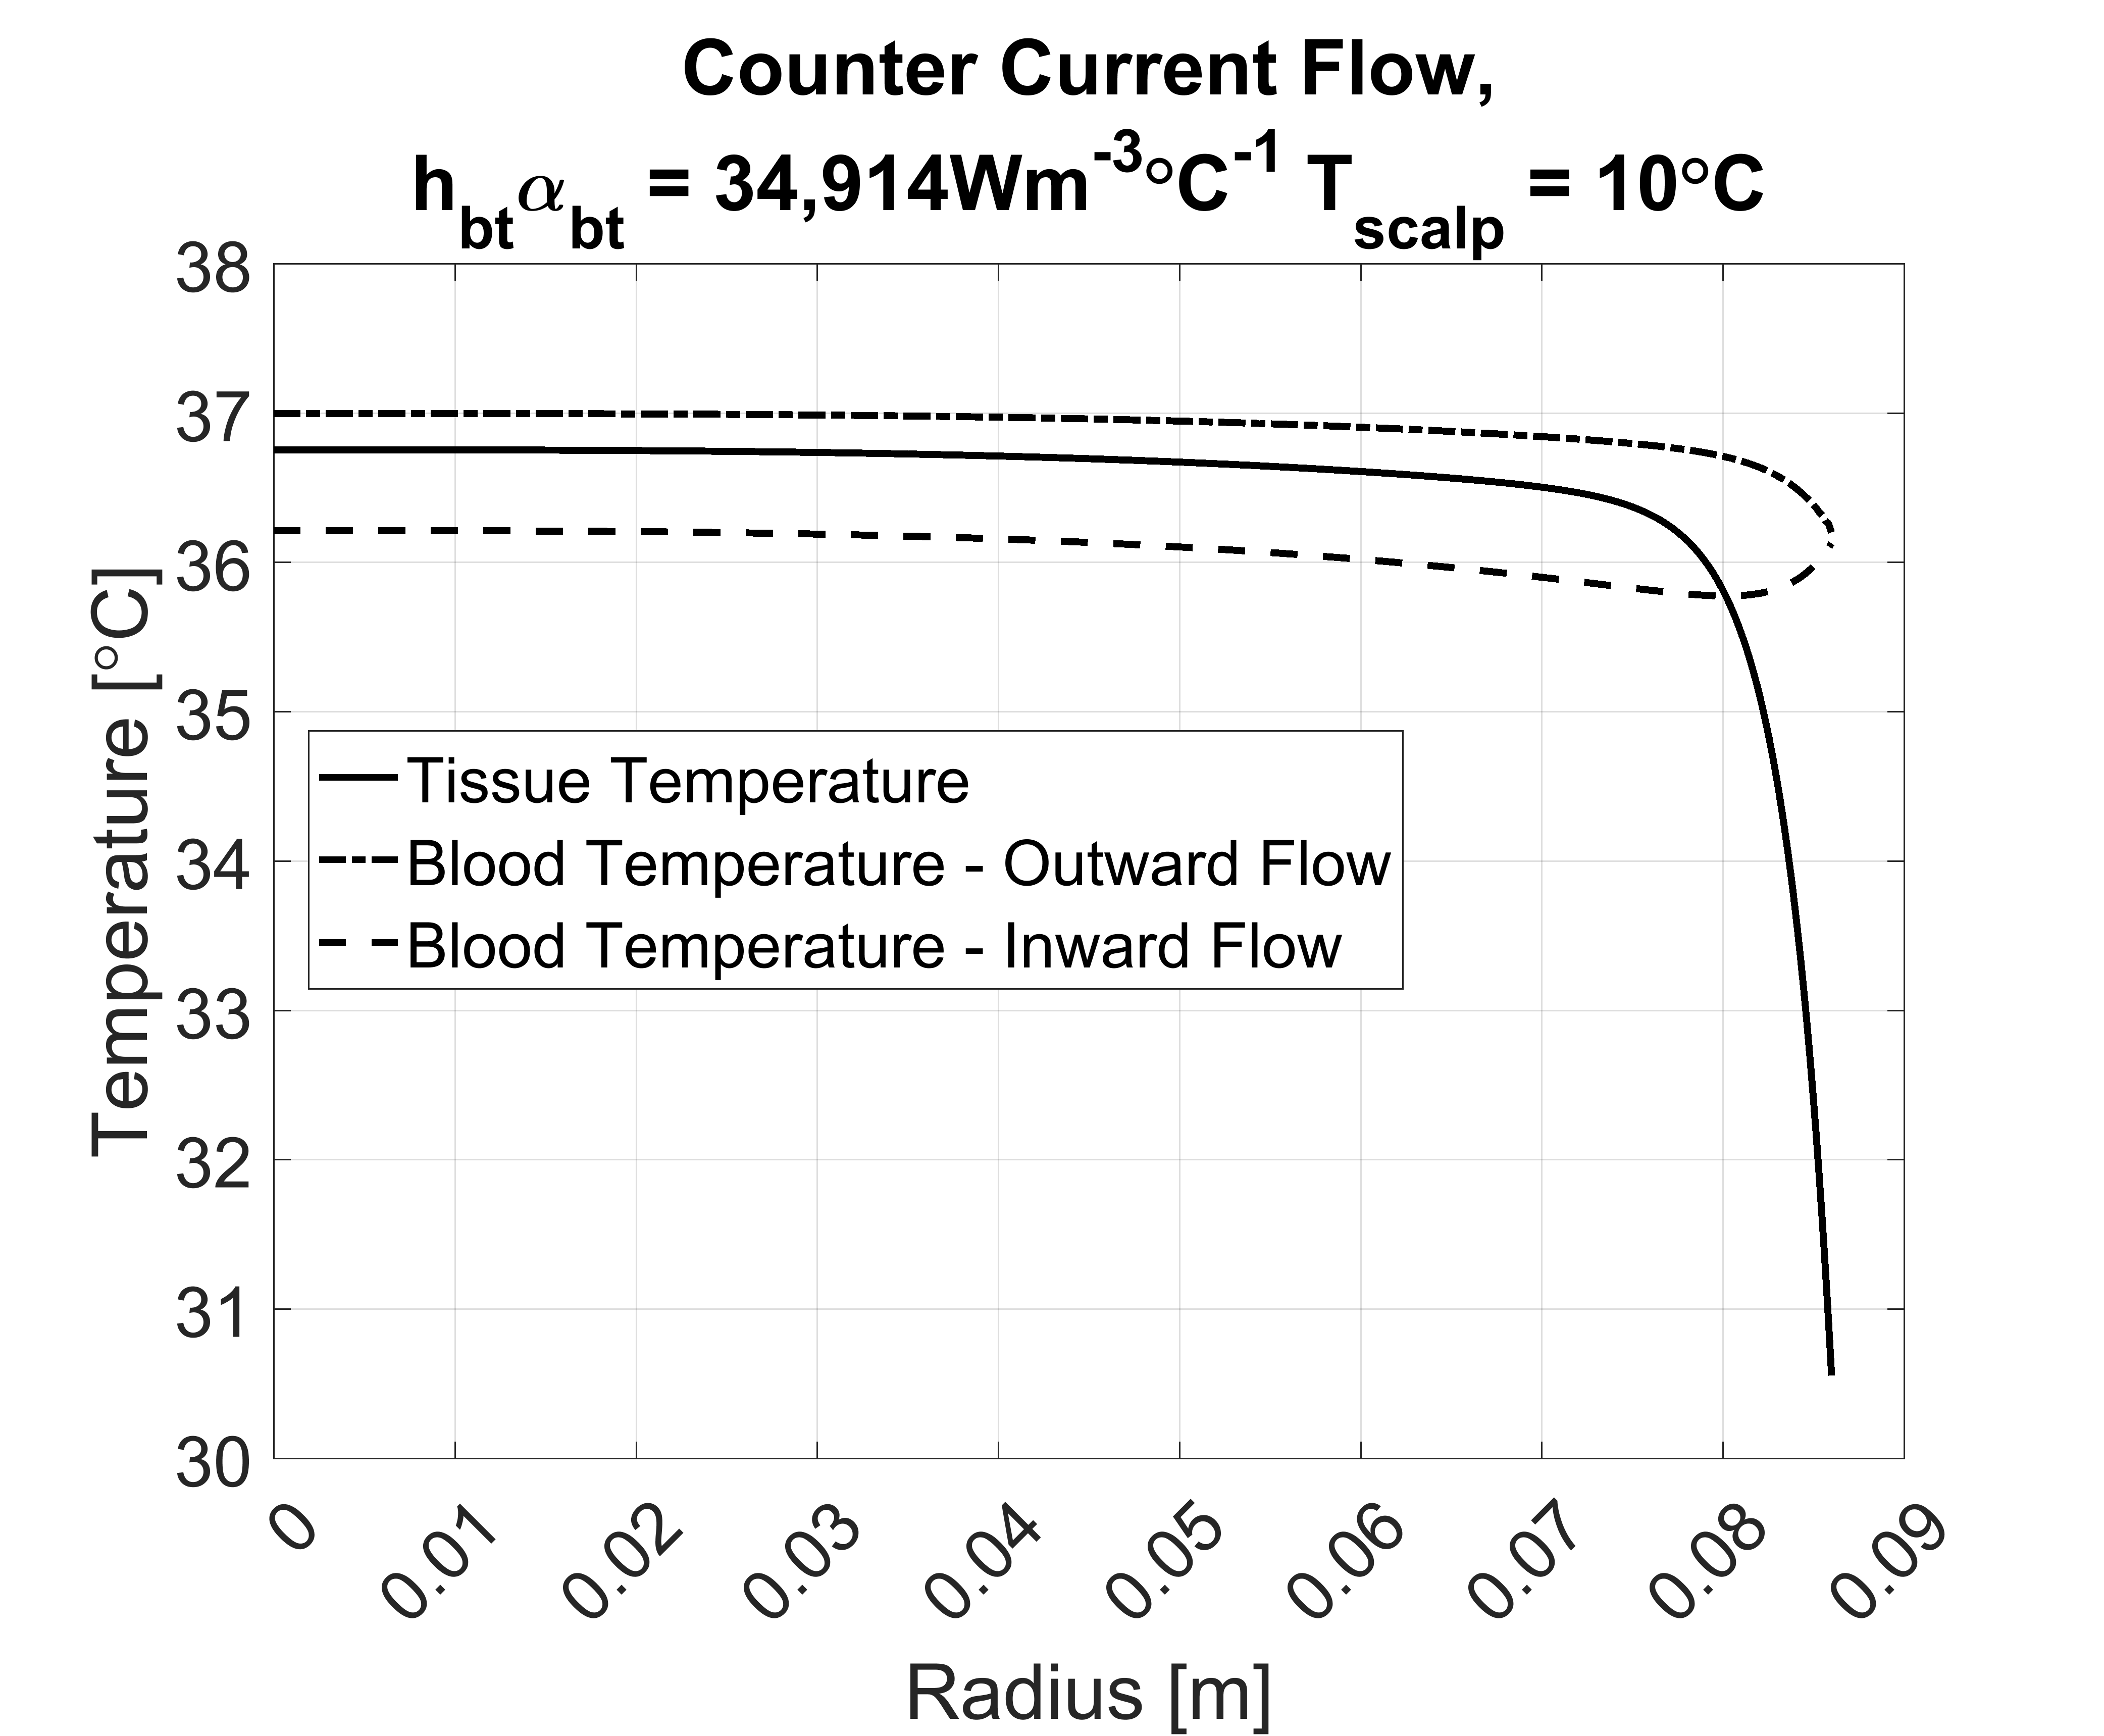
\includegraphics[width=\textwidth]{1DHemisphere/figure11}
	\end{subfigure}
	\caption[Radial temperature distributions for the Counter-Current model with $h_{bt}\alpha_{bt} = \text{34,914}W/m^{3}/^{o}C$ for $T_{scalp}=36.5^{o}C$ and $T_{scalp}=10^{o}C$ .]{Radial temperature distributions for the Counter-Current model with $h_{bt}\alpha_{bt} = \text{34,914}W/m^{3}/^{o}C$ for $T_{scalp}=36.5^{o}C$ (left) and $T_{scalp}=10^{o}C$ (right). Outward flow is directed from the hemisphere centre to the surface radially, whereas the inward flow is directed from the surface to the hemisphere centre radially.}
	\label{fig:Results5}
\end{figure}

Figure~\ref{fig:Results5} shows the temperature profiles for the Counter-Current flow model at $h_{bt}\alpha_{bt} = \text{34,914}W/m^{3}/^{o}C$ under normal and cooling conditions. Here, the profiles for the blood temperatures are shown and it can be seen how they vary with surface temperature. With $T_{scalp} = 36.5^{o}C$, the maximum blood temperature at the core is $37.27^{o}C$ which is slightly shy of the theoretical $0.3^{o}C$ increase expected from metabolism due to surface heat transfer. However, the average tissue temperature is $37.31^{o}C$, comparable to the expected temperature. This in contrast to the previous two-phase model at $h_{bt}\alpha_{bt} = \text{34,914}W/m^{3}/^{o}C$ where the tissue temperature reached higher temperatures due to the required thermal driving force between blood and tissue.

After cooling, the model displays an average temperature drop of $1.27^{o}C$ with a minimum reduction of $0.53^{o}C$. Although there is less of a temperature drop compared to the solely inward flow profile previously, it is comparable to the temperature drop of the inward flow for the Wulff/Klinger model.  

\begin{figure}[h]
	\centering
	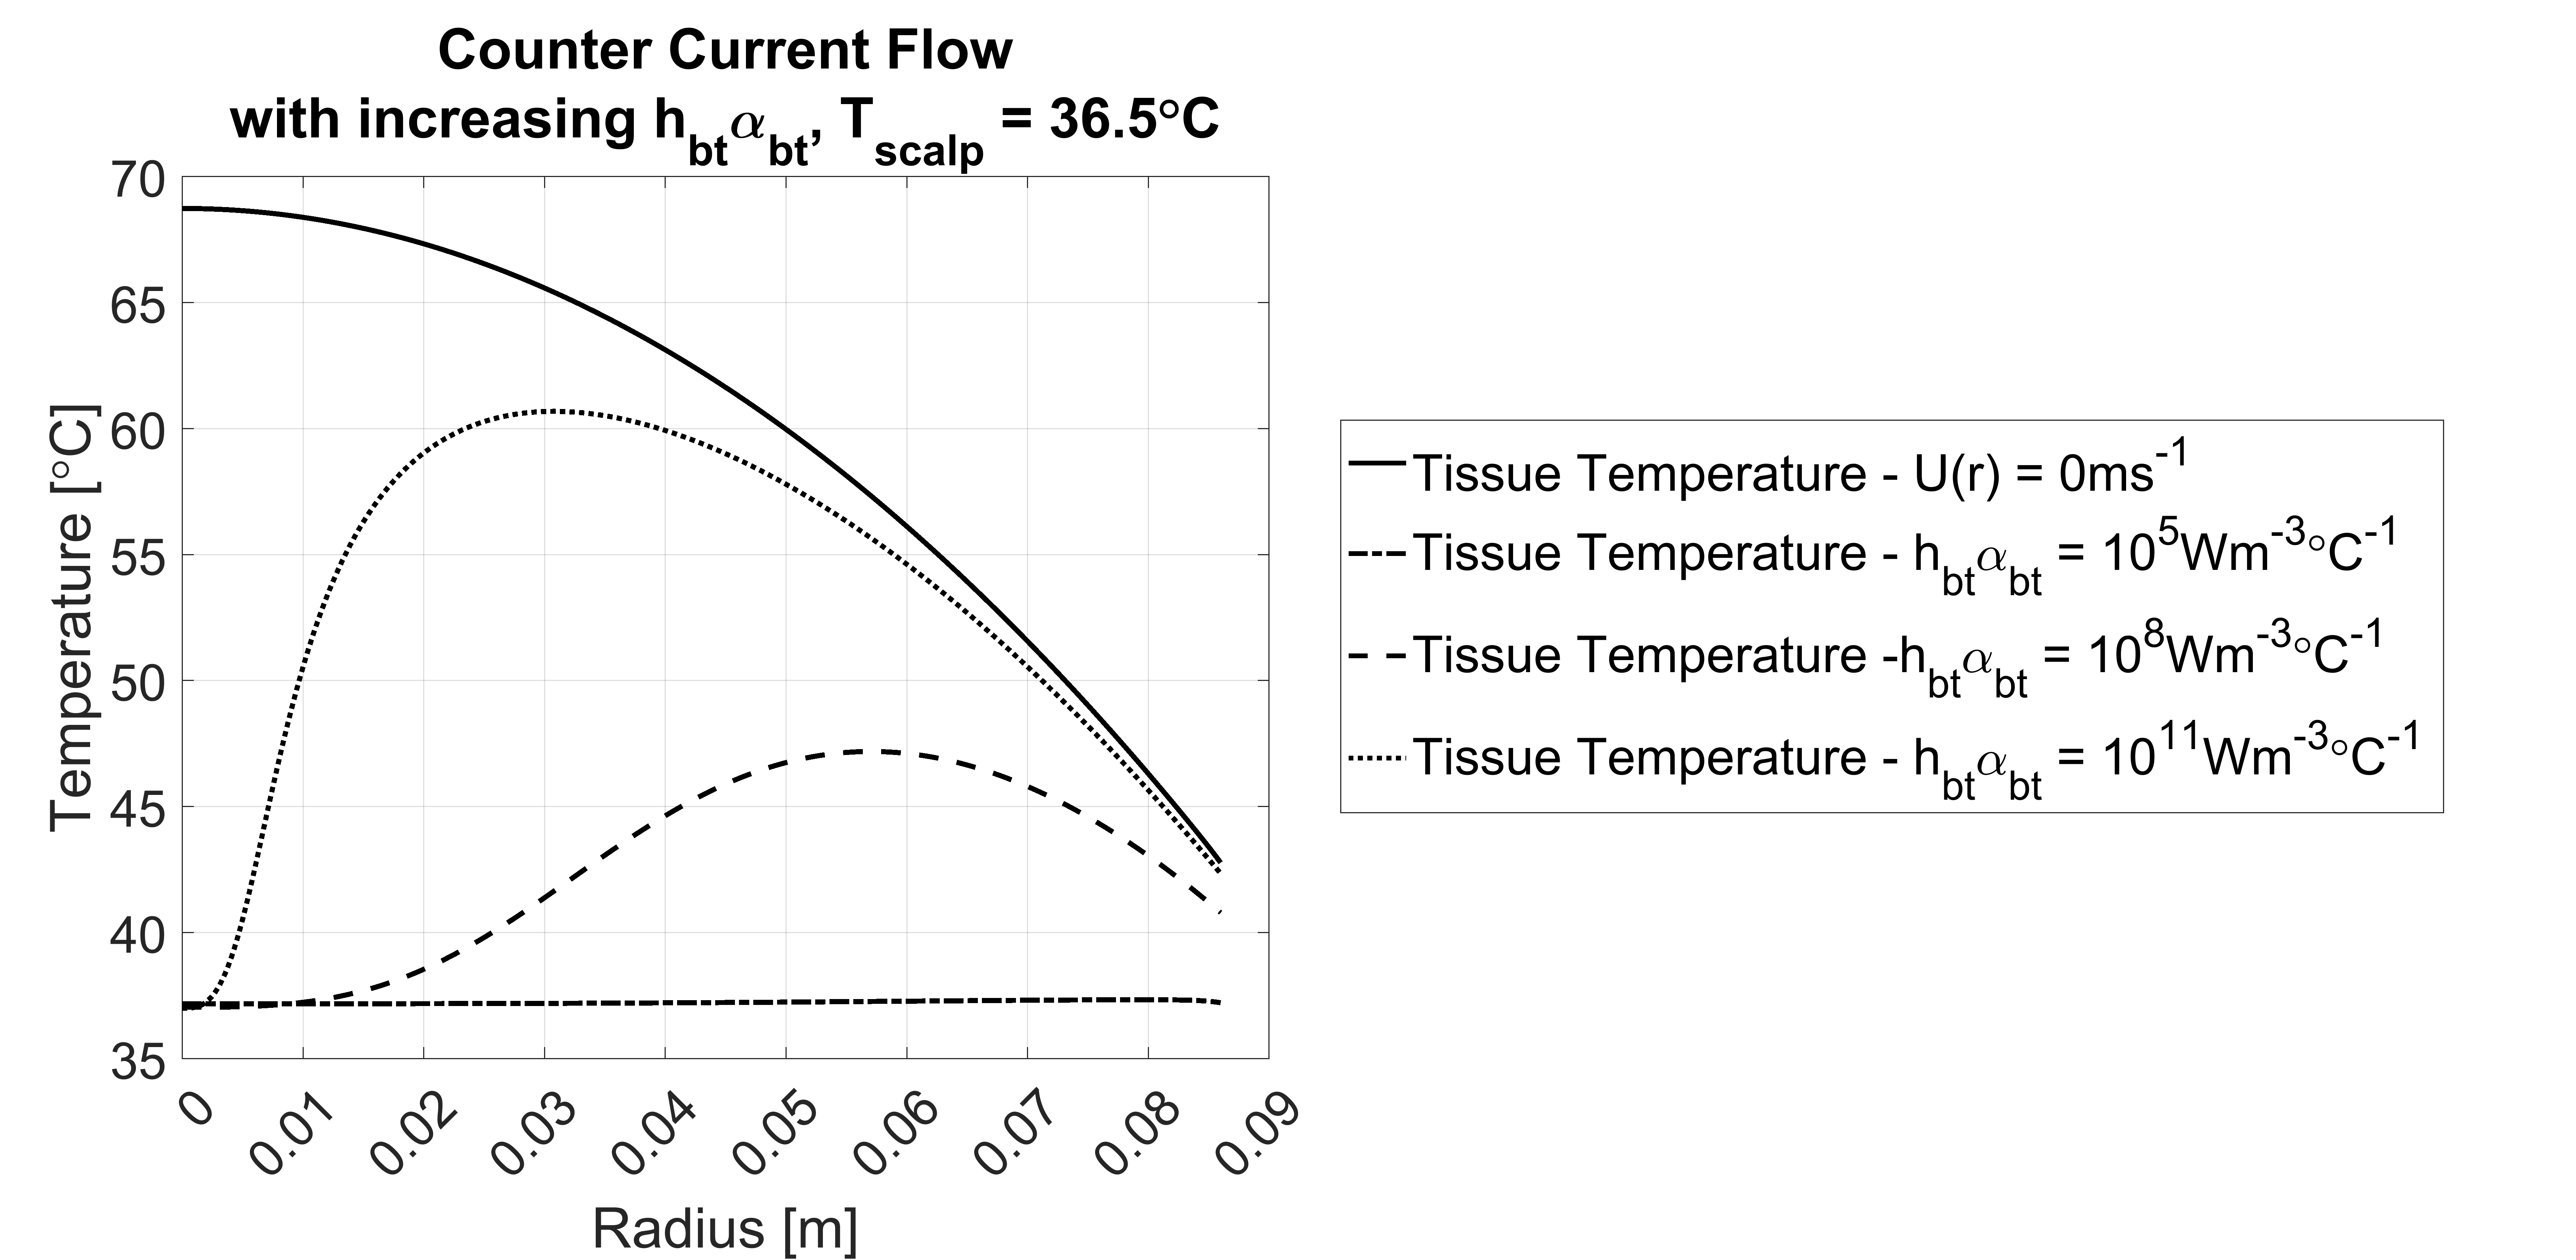
\includegraphics[width=0.85\textwidth]{1DHemisphere/figure12}
	\caption[Radial temperature distributions for the Counter-Current model with various values for $h_{bt}\alpha_{bt}$ with $T_{scalp}=36.5^{o}C$ compared to radial temperature profile a purely conductive model]{Radial temperature distributions for the Counter-Current model with various values for $h_{bt}\alpha_{bt}$ with $T_{scalp}=36.5^{o}C$ compared to radial temperature profile a purely conductive model ($U(r)=0m/s$).}
	\label{fig:Results6}
\end{figure}

Figure~\ref{fig:Results6} shows the temperature profiles for the Counter-Current flow model at increasing $h_{bt}\alpha_{bt}$ under normal scalp temperature conditions. The temperature ranges for $h_{bt}\alpha_{bt} = 10^{8}W/m^{3}/^{o}C$ and above are far outside the expected values for cerebral tissue temperatures. It can be seen that the profiles approach the profile for pure conduction ($U(r) = 0m/s$) as $\lim_{h_{bt}\alpha_{bt}\to\infty}$. This demonstrates that, although the profiles in Figure~\ref{fig:Results5} appear to fall within expected values, the accuracy of the model relies largely on the value for $h_{bt}\alpha_{bt}$.

\subsection{Conclusion}

The results from these 1-Dimensional trials demonstrate that tissue temperature is a function of directional blood flow. This agrees with the criticisms of Pennes Bioheat Equation raised by Wulff \cite{wulff1974energy} and Klinger \cite{klinger1978heat}. The effect of cooling is dependent on the orientation of blood velocity, with flow from the surface to the centre of the brain providing more cooling overall than the opposite direction. 

Combining outwards and inwards flow within the counter-current model produced a result that showed an average temperature matching the expected temperature of $37.3^{o}C$ under normal scalp conditions yet showed a remarkable drop of $1.37^{o}C$ drop in temperature throughout the brain after cooling. This gives weight to the argument that core brain temperature can be reduced through the scalp due to convective effects of blood flow. However, due to the breakdown of the model at increasing inter-domain heat transfer, shown in Figure~\ref{fig:Results6}, the results of this particular model are questionable. 

Throughout all these models, rotational symmetry was preserved and all flow occurs in the radial direction towards or away from the cooling surface. In reality, cerebral blood flows are much more complex and will contain effects not included in this model. Because of this, expansion of the model into three dimensions is required to fully explore the effects of blood flow on cerebral temperatures.

\section[3D Hemispherical Model]{{\Large 3D H}emispherical {\Large M}odel}
\fancyhead[RO]{\makebox[1cm][r]{\fontfamily{ppl}\small\thesection{ -- }\scriptsize\MakeUppercase{{\small3D-H}emispherical {\small M}odel}}\enskip$\mid$\makebox[1cm][l]{\enskip\fontfamily{ppl}\thepage}}

The above equations are limited to radial 1-Dimensional flow and heat transfer which is a large oversimplification of the flows within the brain. In order to better explore the convective heat transfer of the brain, the models need to be expanded into three dimensions. To accomplish this, similar boundary conditions are imposed on a 3-Dimensional hemisphere.

\subsection{Theory}

Additional parameters need to be included to solve the 3-Dimensional system. Whereas in the 1-Dimensional system, the flowrate is defined by a pre-defined mass flowrate and the corresponding radial flux in Equation~\ref{Eq:SphericalVelocity}, the 3-Dimensional system requires specific inlets and outlets and a momentum sink to properly bound the model. 

\begin{figure}[h]
	\centering
	\begin{subfigure}[b]{0.45\textwidth}
		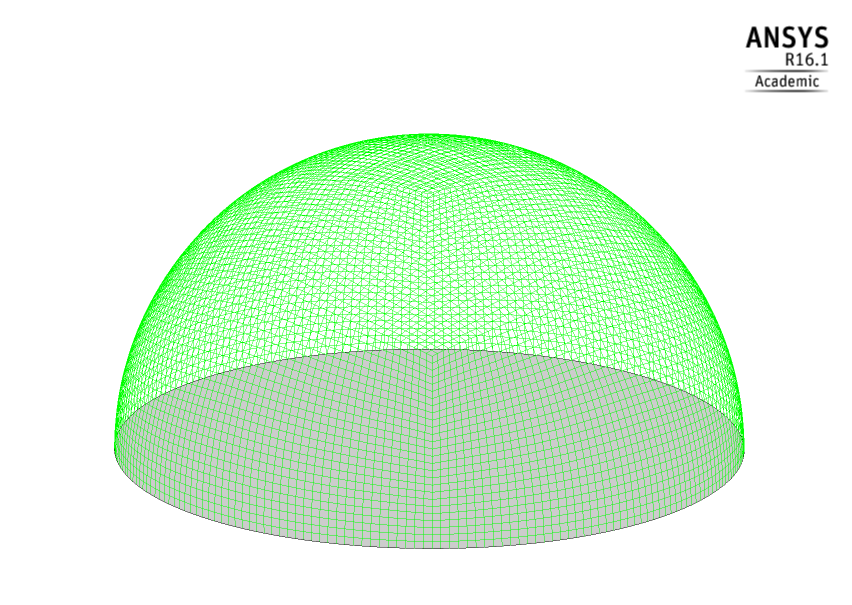
\includegraphics[width=\textwidth]{3DHemisphere/HemisphereMesh}
	\end{subfigure}
	\begin{subfigure}[b]{0.45\textwidth}
		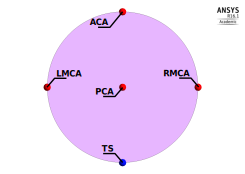
\includegraphics[width=\textwidth]{3DHemisphere/InletOutletLabels}
	\end{subfigure}
	\caption[Mesh and domain for 3D hemispherical model with the location of inlets and outlets]{Left: Mesh used in 3D Hemispherical model. Right: locations of inlets on the base of the hemisphere. Red dots indicate inlets and blue dots indicate outlets. The inlets and outlets are the anterior cerebral arteries (ACA), the left (LMCA) and right (RMCA) middle cerebral arteries, the posterior cerebral arteries (PCA) and the transverse sinuses (TS).}
	\label{fig:InletOutlet3DHemisphere}
\end{figure}

Various combinations of inlets and outlets were considered with the primary goal of distributing the blood evenly throughout the model. These inlets and outlets were implemented using source points which could be inputted manually within the simulation set-up. Four inlets and one outlet was chosen which represent the major vasculature within the brain: the anterior cerebral arteries, the left and right middle cerebral arteries, the posterior cerebral arteries and the transverse sinuses at the rear of the brain. For simplicity, inlet flowrate was divided equally between these points. The domain and the locations of the inlets are depicted in Figure~\ref{fig:InletOutlet3DHemisphere}.

The brain tissue was assumed to be a porous material. The momentum loss associated with travelling through this medium was assumed to adhere to Darcy's Law:

\begin{equation}
\frac{\partial P}{\partial l}=-\frac{\mu_{b}}{\kappa}U
\end{equation}

Where $P$ is pressure, $l$ is the length between voxels, $\mu_{b}$ is the viscosity of blood which is assumed to be $3.5mPa{\cdot}s$, and the permeability, $\kappa$, is given by:

\begin{equation}
\kappa = \frac{\epsilon_{b}{D_{c}}^{2}}{32\tau}
\end{equation}

Where $D_{c}$ is the capillary diameter and is assumed to be $10\mu m$. The variable, $\tau$, represents the tortuosity of the capillaries, which is defined as the ratio between the length of capillary vessel and the distance between the two end points. The larger this value, the curvier and more convoluted the vessel is. This is assumed to be an arbitrary value of $2.5$. 

The system was modelled in Ansys CFX $16.0$. The velocity profile was solved initially and then the temperature profile was solved independently afterwards using the previously solved velocity profile. This was to prevent any deviance in velocity profile from different temperature trials. It also sped up the rate of convergence significantly. Negligible error is expected from the de-coupling of the solver as the physical values are constants. Both solutions were solved to a residual value of $10^{\smallminus4}$. For simplicity, the automatic time-step option was used, however, for the temperatures, this was increased by a factor of 1000 to speed up temperature convergence with negligible effect on results. 

\subsection{Results}

For the sake of brevity, only a single result is displayed here. It serves to highlight the drawbacks of this implementation. Figure~\ref{fig:SuperficialVelocity} shows the superficial velocity of blood and Figure~\ref{fig:3DTemperature} shows the temperature profile with a scalp temperature set at $36.5^{o}C$.

\begin{figure}[h]
	\centering
	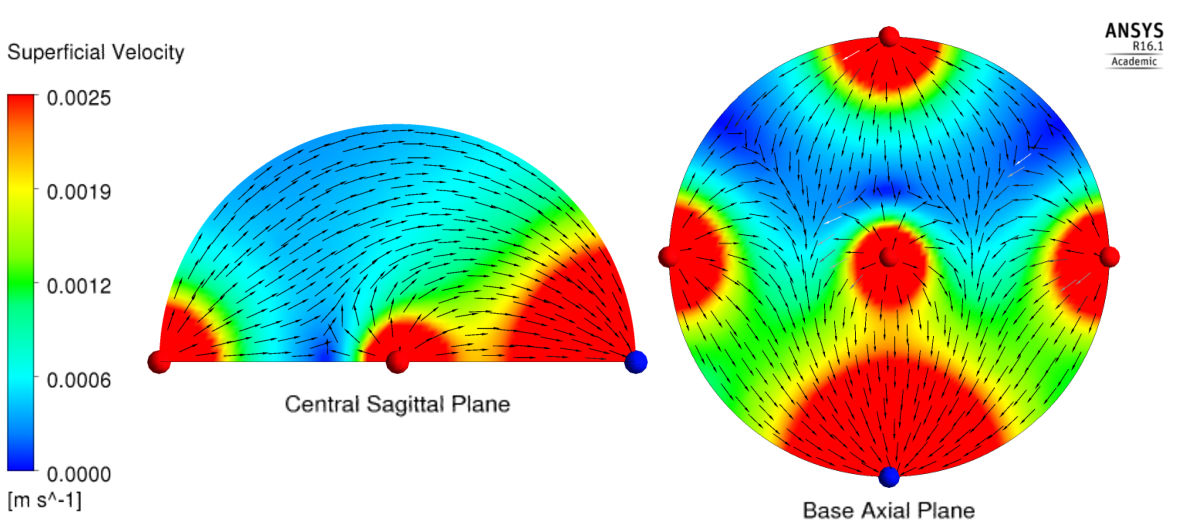
\includegraphics[width=0.8\textwidth]{3DHemisphere/SuperficialVelocity}
	\caption[Velocity profiles for 3D Hemispherical model]{Velocity profiles for 3D Hemispherical model.}
	\label{fig:SuperficialVelocity}
\end{figure}

\begin{figure}[h]
	\centering
	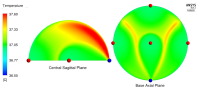
\includegraphics[width=0.8\textwidth]{3DHemisphere/Temperature2}
	\caption[Temperature profiles for 3D Hemispherical model with $T_{scalp}=36.5^{o}C$]{Temperature profiles for 3D Hemispherical model with $T_{scalp}=36.5^{o}C$.}
	\label{fig:3DTemperature}
\end{figure}

As seen in Figure~\ref{fig:SuperficialVelocity}, assigning inlets and outlets in arbitrary locations creates regions with large variances in flowrates. This is due to all the blood entering the system through a small number of inlet points, and the low permeability of the porous media limiting the distribution to distant areas. In Figure~\ref{fig:3DTemperature}, it can be seen that regions of lower velocities towards the surface are more susceptible to temperature changes. This agrees with literature that the blood flow to a region alleviates the temperature rise due to metabolism \cite{sukstanskii2006theoretical}, however, it is not expected that such regions of decoupled blood flow and metabolism exist within the brain. A good agreement between flow and metabolism is therefore warranted when dealing with bioheat models. 

To achieve this agreement within a hemisphere inlets and outlets could be moved to attempt to distribute the flow around the domain more evenly. Additionally, the number of source or sink points could be increased for the same effect. Alternatively, the permeability parameters could be varied in different regions to encourage the blood to spread out as it moves towards the outlets. However, these facets could be altered to no end without producing a realistic representation of blood flow in the brain. Instead, a more physical basis can be implemented whereby the distribution of blood is achieved using embedded blood vessels.

\section[Full 3D Model with Vasculature]{{\Large F}ull {\Large 3D} {\Large M}odel with {\Large V}asculature}
\fancyhead[RO]{\makebox[1cm][r]{\fontfamily{ppl}\small\thesection{ -- }\scriptsize\MakeUppercase{{\small F}ull {\small 3D} {\small M}odel with {\small V}asculature} }\enskip$\mid$\makebox[1cm][l]{\enskip\fontfamily{ppl}\thepage}}

To create a more realistic flow pattern, the model requires vasculature to properly distribute the blood around the brain without resorting to arbitrary source points. This can be done by creating 3D domains of blood vessels taken from scans and embedding them within the tissue domain. Imposing a fluid domain on the vessels with a porous domain in the tissue should allow the blood to distribute more freely. As the two vessel domains are not connected, the blood would have to pass through the tissue at some point. It is expected that due to the high momentum sink term, the blood should take a variety of paths to reach the outlet. 

\subsection{Creating Vasculature}

\begin{figure}[h]
	\centering
	\includegraphics[width=0.6\textwidth]{3DFullVessels/STLs1}
	\caption[STLs used of head, brain, arteries and veins visualised in Autodesk Meshmixer]{STLs used of head, brain, arteries and veins visualised in Autodesk Meshmixer.}
	\label{fig:STLs1}
\end{figure}

In order to facilitate the distribution of blood throughout the model, realistic blood vessels are required. Drawing vessels by hand within the domain is inaccurate and inefficient. Instead, it is possible to extract geometries from scans such as angiograms and venograms. 

Scans were obtained without patient information and they displayed vessels in the form of image slices. These slices showed the intensity of measured tissue with the highest values being the blood inside vessels. This data had to be isolated and then rendered in 3D. The isolation was performed by establishing the threshold values for the bands of intensity corresponding to the vessels. The surface could then be extracted by identifying pixels that do not have neighbours in all 26 directions (i.e.\ sharing an edge, face, or corner). This usually created a jagged surface due to the resolution of the scans (2mm pixel size) which could cause unwanted flow effects within the vessel. Ideally, the resultant surfaces should be smoother.

To smooth the vessel surfaces, an alternative approach to surface creation was used. Instead of extracting the surface, the centrelines of the vessels were extracted to form a skeleton of the vessel using open source software \cite{kroon2011accurate}. If diameters were measured at points throughout the skeleton manually, then a circular surface could be lofted over the it to produce a surface that is perfectly smooth. Although still unrealistic, this process made the meshing easier and removed the rough surface that could affect results.

Initially, the lofting of the surface was accomplished manually through CAD based software (Autodesk Inventor). Due to the number of branches within the vessel structure, the process was tedious and difficult. The output of the skeletal creation produced branches but did not provide full connectivity. This too had to be rectified manually. The venous vessel structure was created in this manner. The arterial tree, when extracted from the original scan was missing posterior communicating arteries within the circle of Willis. This was rectified by producing two straight cylindrical connecting branches.

These vessels were placed into a 3D domain of a brain and head model. They were manually scaled and positioned within the domains. This could lead to errors in positioning but it functioned for preliminary studies as long as there was sufficient interface area to properly distribute the blood between domains.

Another hindrance in producing this structure was the mesh creation from the embedded surfaces. Due to the numerous intersections between domains, a large number of independent volumes were created. These had to be individually assigned their corresponding domain. Overall, this surface and mesh creation process represented a large bottleneck in the development of the model.

\begin{figure}[h]
	\centering
	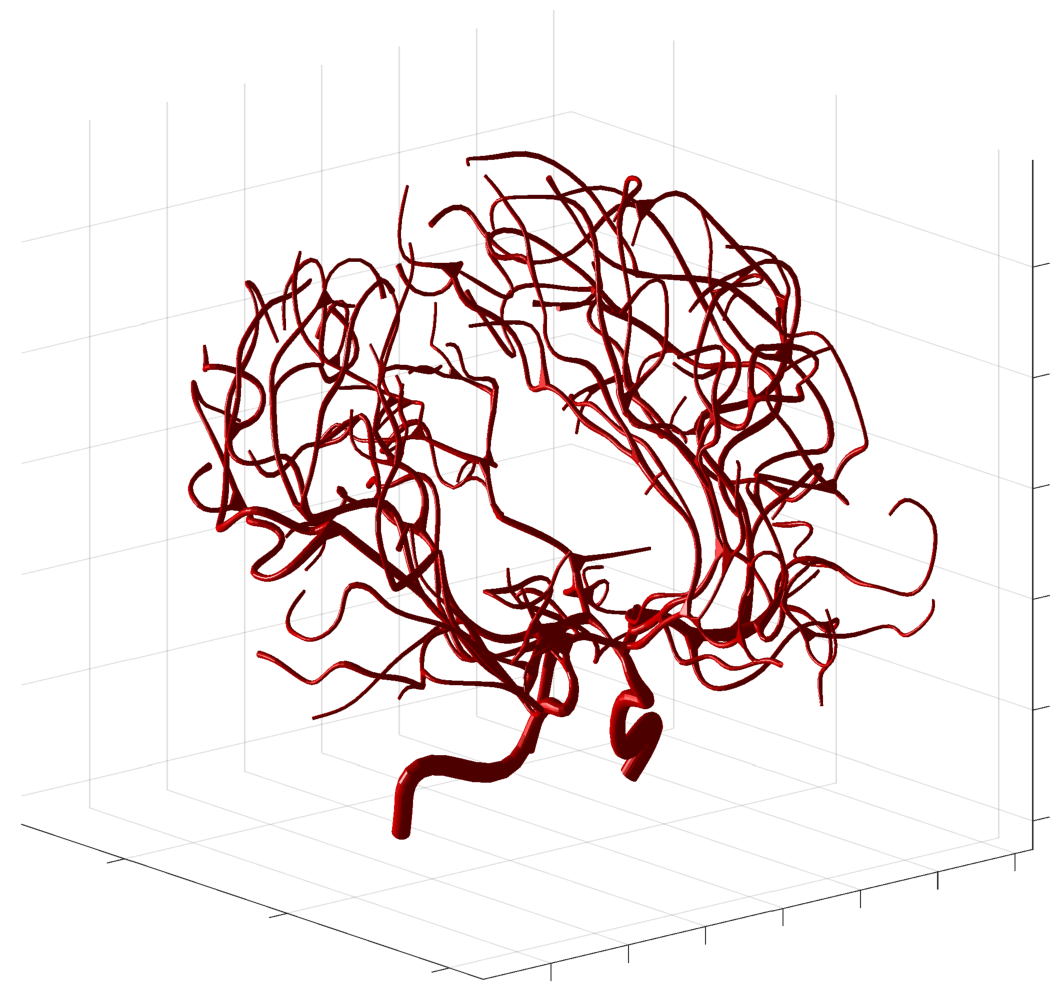
\includegraphics[width=0.6\textwidth]{3DFullVessels/arteries3D1}
	\caption[Full arterial tree STL generated automatically via software using the input data from BraVa (file: BG001)]{Full arterial tree STL generated automatically via software using the input data from BraVa (file: BG001).}
	\label{fig:3Darteries}
\end{figure}	

\begin{figure}[h]
	\centering	
	\begin{subfigure}[b]{0.45\textwidth}
		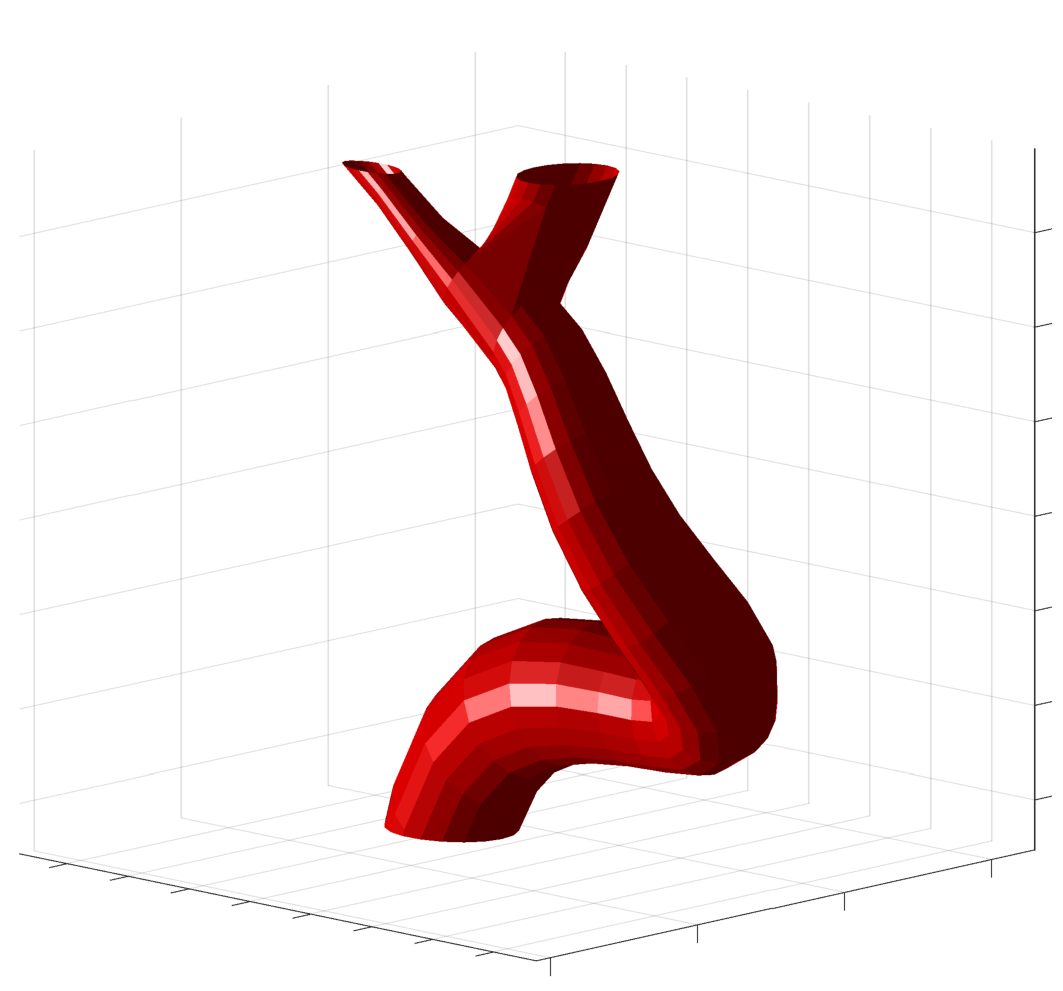
\includegraphics[width=\textwidth]{3DFullVessels/arteries3D2}
	\end{subfigure}
	\begin{subfigure}[b]{0.45\textwidth}
		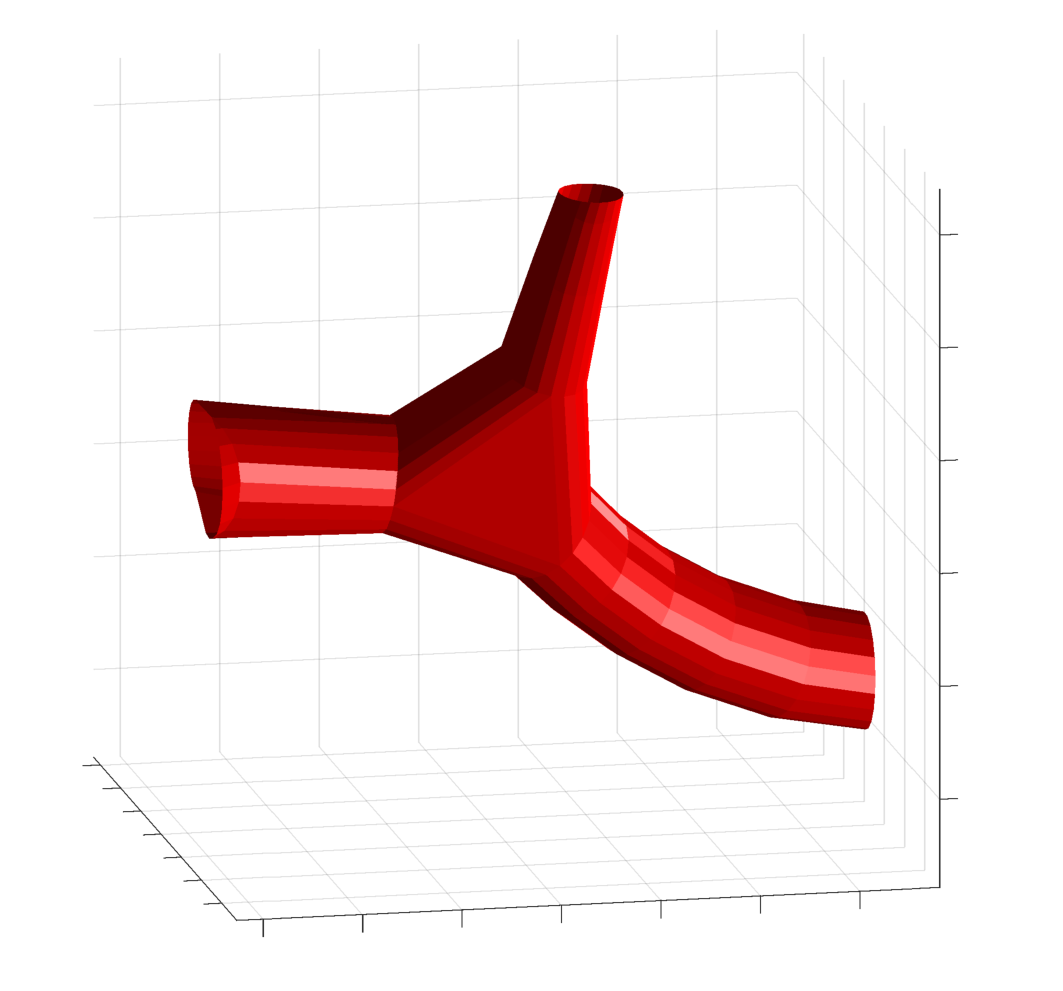
\includegraphics[width=\textwidth]{3DFullVessels/arteries3D3}
	\end{subfigure}
	\caption[Close up views of STL creation via software]{Close up views of STL creation via software. The right-hand figure depicts the basic lofting used to connect bifurcations.}
	\label{fig:3DarteriesParts}
\end{figure}

Subsequently, denser vasculature was obtained from an online database of cerebral arterial vessels, named BraVa (located at [\texttt{http://cng.gmu.edu/brava}]) \cite{wright2013digital}. This database contained various trees stored as line segments with connectivity. However, these datasets were too complex to perform the circular lofting manually. Instead, software was written to complete this automatically based on methods used to create a cerebral vascular atlas \cite{nowinski2009new}. This software performed the repetitive task of drawing circles and creating surfaces across all branches of the dataset. It also smoothed the data by performing a moving average over the spatial locations and diameters as in Nowinski et al. \cite{nowinski2005informatics} to prevent jagged branches. The resultant STL file is shown in Figure~\ref{fig:3Darteries}. Close-up portions of this tree are shown in Figure~\ref{fig:3DarteriesParts}. For the bifurcations, a simple connection of points between intersecting branches was used, forming a triangular loft. Although a rudimentary method, it functioned for the purposes of these preliminary studies.

\subsection{Set-Up}

\begin{figure}[h]
	\centering	
	\begin{subfigure}[b]{0.45\textwidth}
		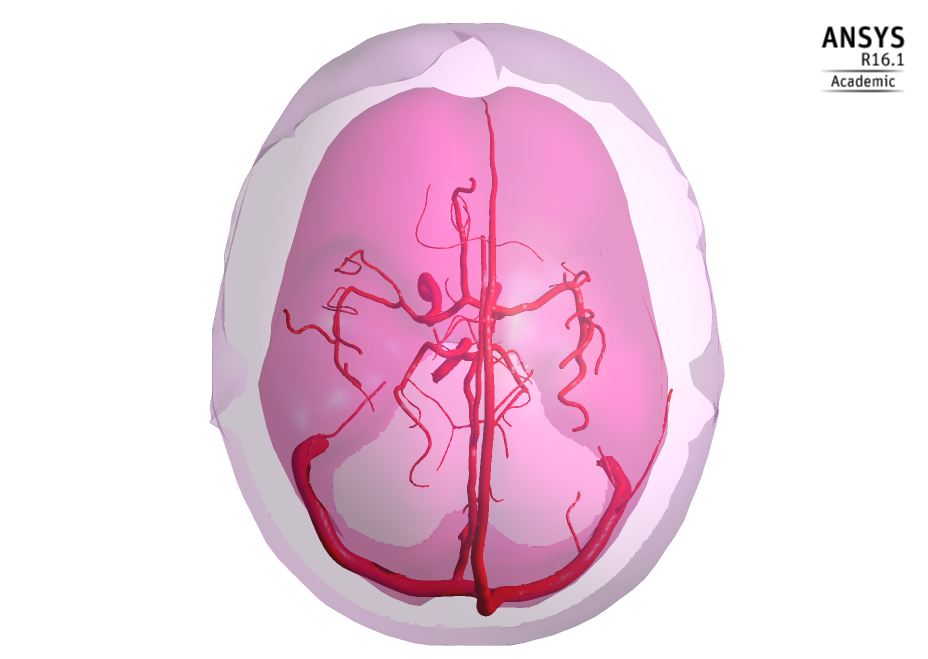
\includegraphics[width=\textwidth]{3DFullVessels/FirstModelTransparency2}
	\end{subfigure}
	\begin{subfigure}[b]{0.45\textwidth}
		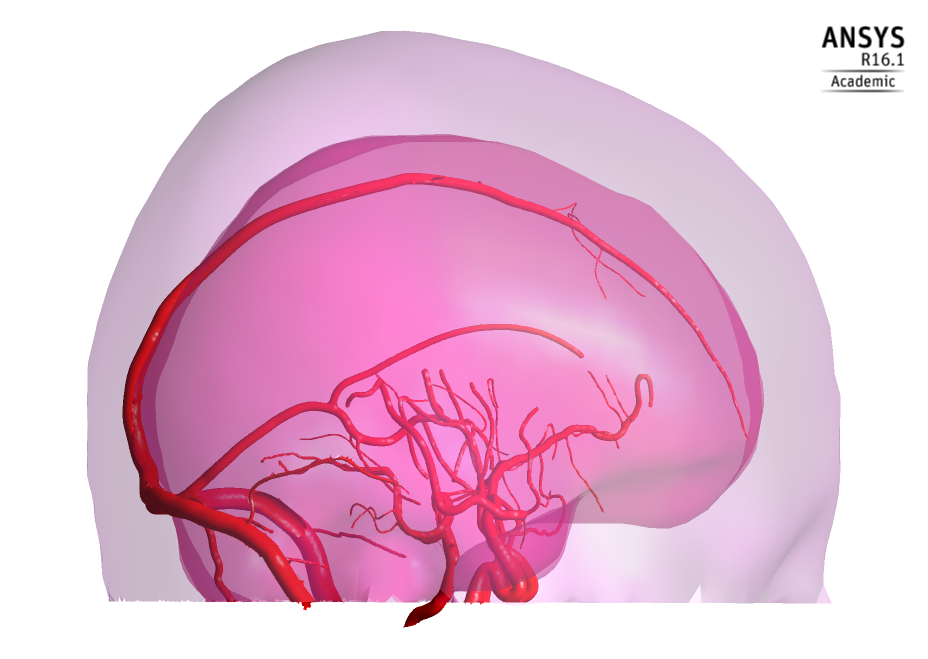
\includegraphics[width=\textwidth]{3DFullVessels/FirstModelTransparency1}
	\end{subfigure}
	\caption[Sparse arterial tree and venous vessel tree embedded within brain and head surfaces]{Sparse arterial tree and venous vessel tree embedded within brain and head surfaces.}
	\label{fig:3DTransparencies1}
\end{figure}

\begin{figure}[h]
	\centering	
	\begin{subfigure}[b]{0.45\textwidth}
		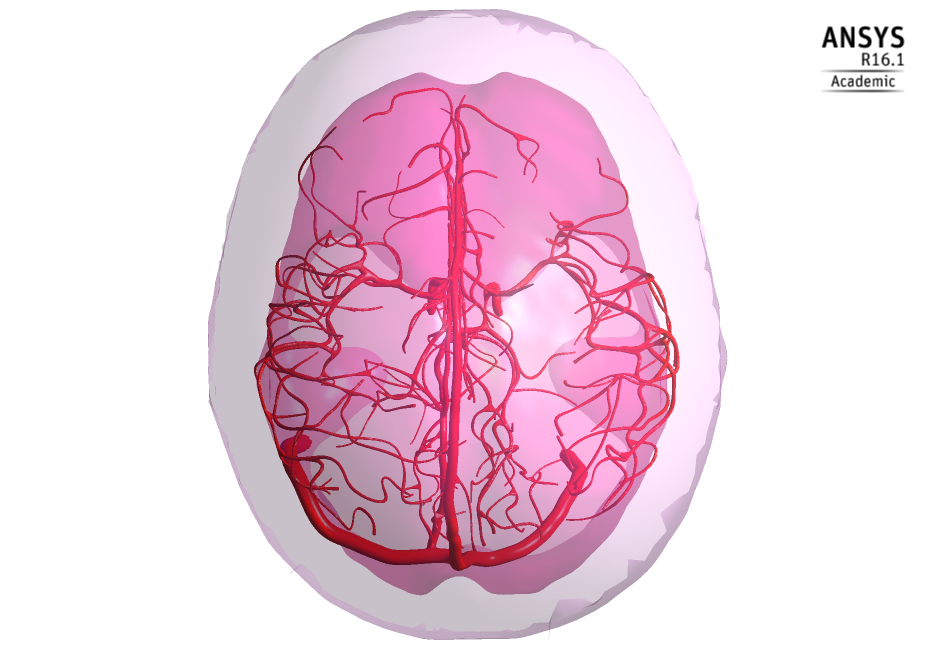
\includegraphics[width=\textwidth]{3DFullVessels/ModelTransparency2}
	\end{subfigure}
	\begin{subfigure}[b]{0.45\textwidth}
		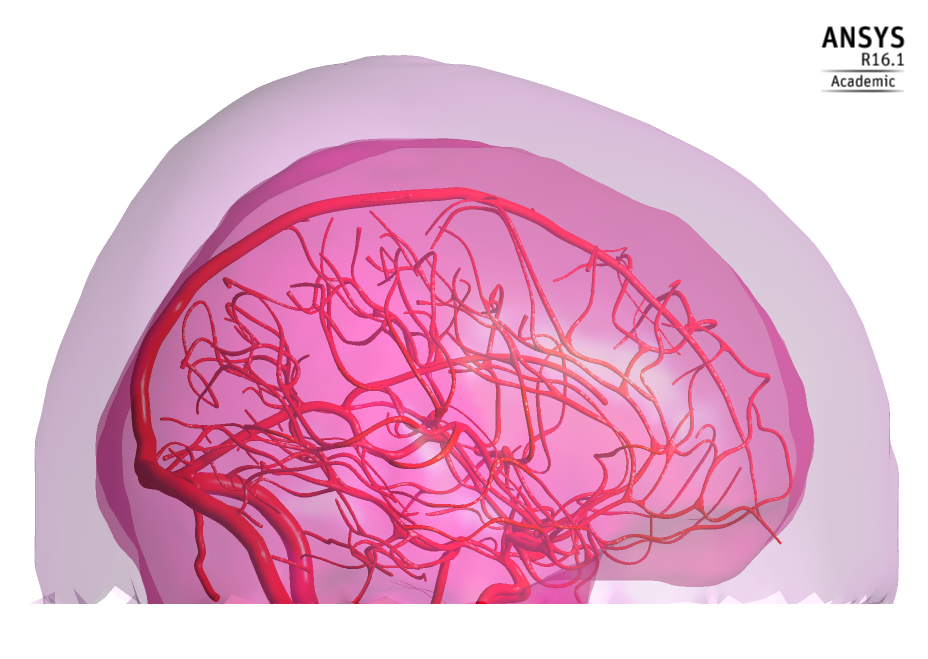
\includegraphics[width=\textwidth]{3DFullVessels/ModelTransparency1}
	\end{subfigure}
	\caption[Dense arterial tree and venous vessel tree embedded within brain and head surfaces]{Dense arterial tree and venous vessel tree embedded within brain and head surfaces.}
	\label{fig:3DTransparencies2}
\end{figure}

Figures~\ref{fig:3DTransparencies1}~\&~\ref{fig:3DTransparencies2} show the embedded vessels in the brain and head domains for sparse and denser sets of arteries respectively. They were positioned manually based on their expected location from on-line anatomy sources. This led to discrepancies such as the transverse sinus not stretching across the entire brain domain in Figure~\ref{fig:3DTransparencies2}. However, the impact from these placement errors was of no consequence in the context of the results shown.

The unstructured meshes to simulate these domains were created using the Octree method in ICEM CFD. The largest element limit was set to $0.5mm$ in the vessel domains (artery and vein) and $20mm$ in the tissue domains (brain and outer-head). This led to $1.25*10^{6}$ total elements in the mesh with the sparse vascular tree and $6.15*10^{6}$ total elements in the mesh with the dense vascular tree.

Inlet flowrates for the arteries were divided up 40\%, 40\%, \& 20\% between the left and right carotid arteries and the basilar artery respectively \cite{tanaka2006relationship}. The two terminations of the transverse sinuses were designated pressure outlets at atmospheric pressure. 

The momentum loss could be altered by adjusting the capillary diameter in order to ensure the resultant pressure drop matched physiological values. However, this could only be performed through trial and error due to the complex vascular geometry. The resultant change in flow did not dramatically alter the results shown below. Therefore, for continuity, the same capillary diameter of $10\mu m$ used in the hemispherical model was used in both models here. 

As with the hemispherical model, the system was solved using Ansys CFX 16.0. Due to the inclusion of neighbouring fluid and porous domains, the solution did not converge. Instead, the expert parameter option `porous cs discretisation' had to be implemented, otherwise the solver proved unstable. This adjusts the pressure at the fluid-porous interface. The default value (2) maintains a constant total pressure at the interface, however, some solutions fail to converge if there is very little flow across the interface. This scenario is most likely present here as much of the flow is tangential to the fluid-porous in the vessels interface. The alternative value (1) uses a constant static pressure at the boundary. Although deemed less realistic, this allowed the solver to converge.

As before, the velocity profile was solved initially and then the temperature profile was solved independently afterwards using the previously solved velocity profile. Negligible error is expected from the de-coupling of the solver. Both solutions were solved to a residual value of $10^{\smallminus4}$. Due to the varying scales of the unstructured mesh and the implementation of different domains types, the time-step was designated automatically by the solver in Ansys CFX. For the thermal solution, increasing this by a factor of 1000 sped up convergence without affecting the numerical accuracy of results. 

\subsection{Results}

As before with the hemispherical model results, for the sake of brevity, a single solution is shown to highlight the drawbacks of this method.

\begin{figure}[h]
	\centering
	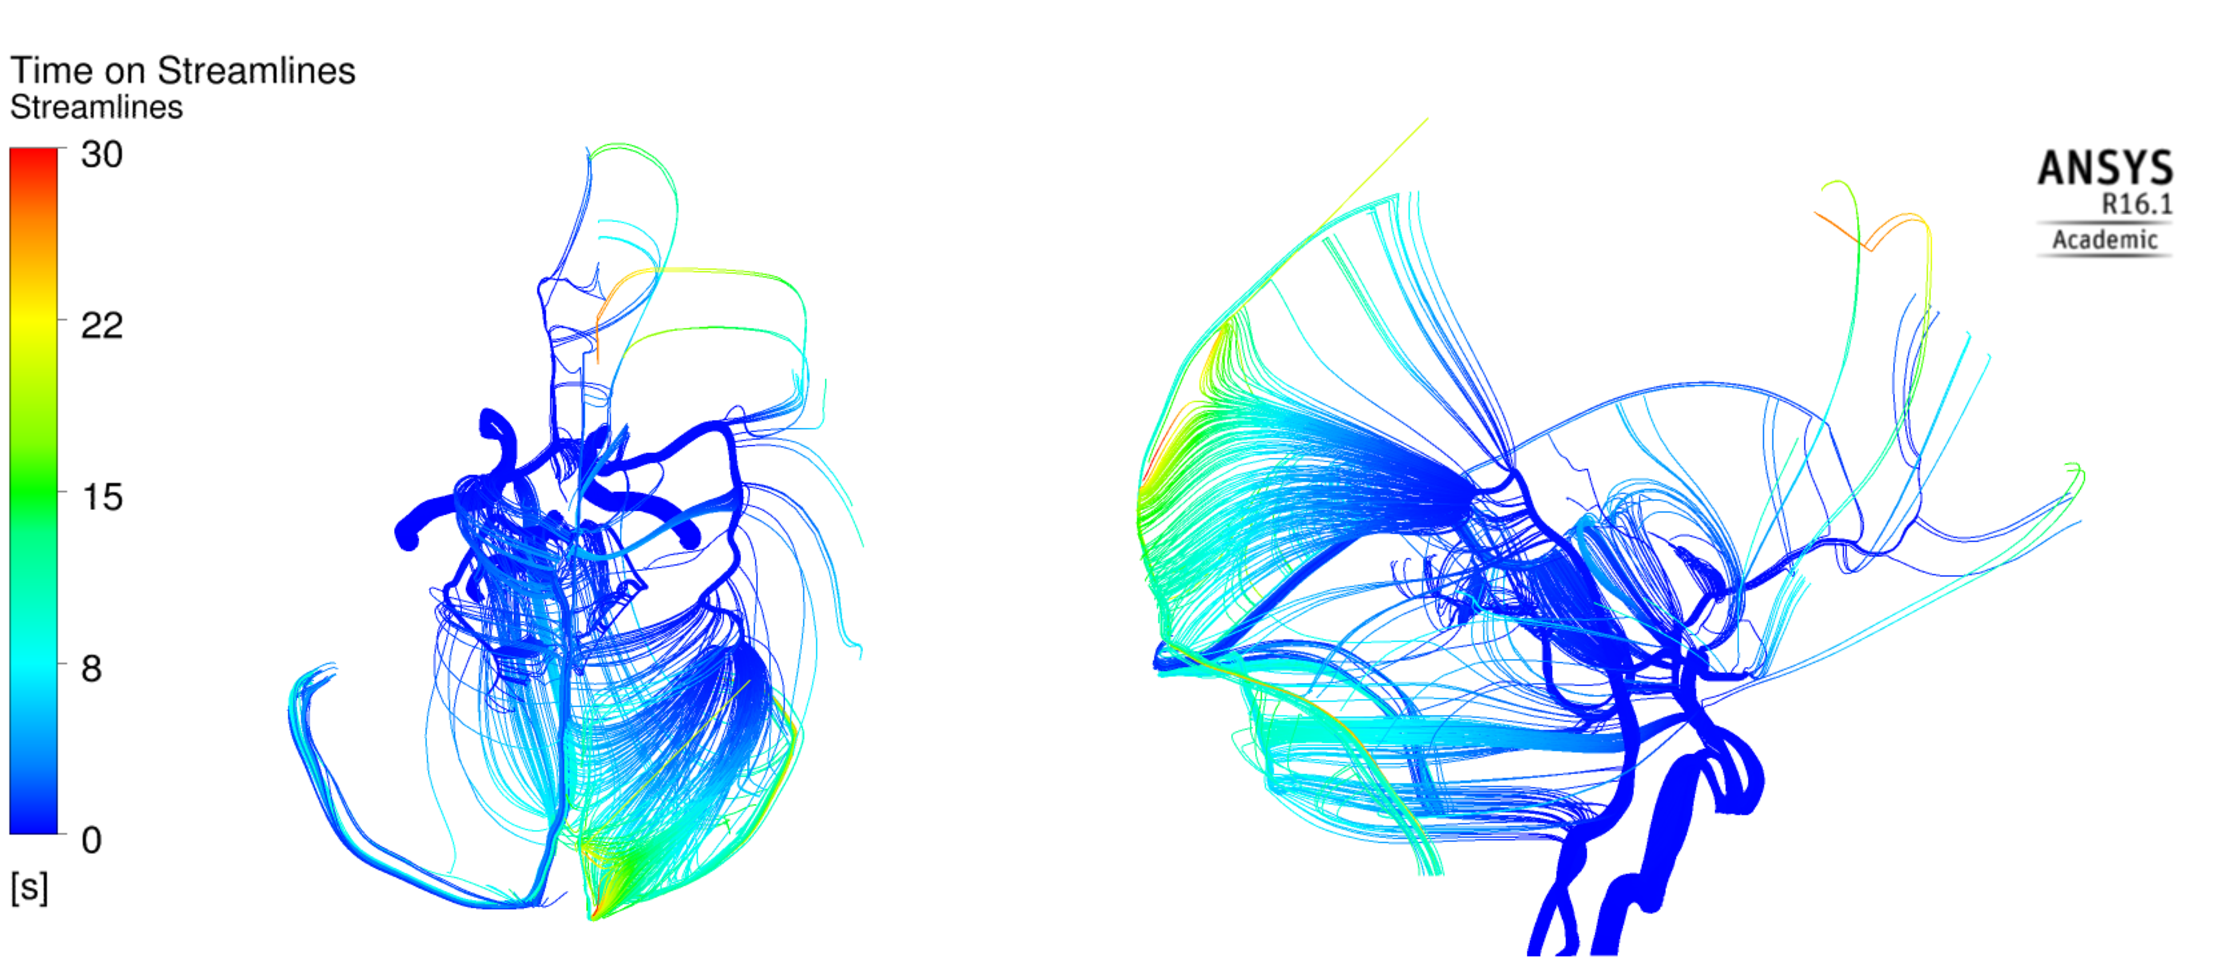
\includegraphics[width=0.9\textwidth]{3DFullVessels/streamlines2}
	\caption[1500 flow streamlines generated randomly spread over the inlet areas for the sparse arterial tree model]{1500 flow streamlines generated randomly spread over the inlet areas for the sparse arterial tree model.}
	\label{fig:streamlines1}
\end{figure}

Figure~\ref{fig:streamlines1} displays streamlines of the resolved flow with the embedded arteries and veins present inside the brain volume. These are randomly generated over the inlet surface to give an idea to the distribution of flow. Although, the domain boundaries are not highlighted here, comparing Figures~\ref{fig:3DTransparencies1}~\&~\ref{fig:streamlines1} shows that the streamlines adhere closely to the structure of the embedded vessels. However, there is a clear gap in streamlines in the superior portion of the brain. This is contrasted with the large concentration of streamlines passing through the posterior portion of the brain. This indicates that the introduction of blood vessels is not distributing the blood as evenly as was hoped.

There are only a finite number of streamlines that can be displayed before the data becomes occluded. They cannot convey an exact flowrate distribution, as shown for the hemisphere model in Figure~\ref{fig:SuperficialVelocity}, but serve as an indication of distribution instead. Therefore, the lack of streamlines in the superior portion of the brain does not necessarily indicate a flowrate of zero in that region.  

\begin{figure}[h]
	\centering
	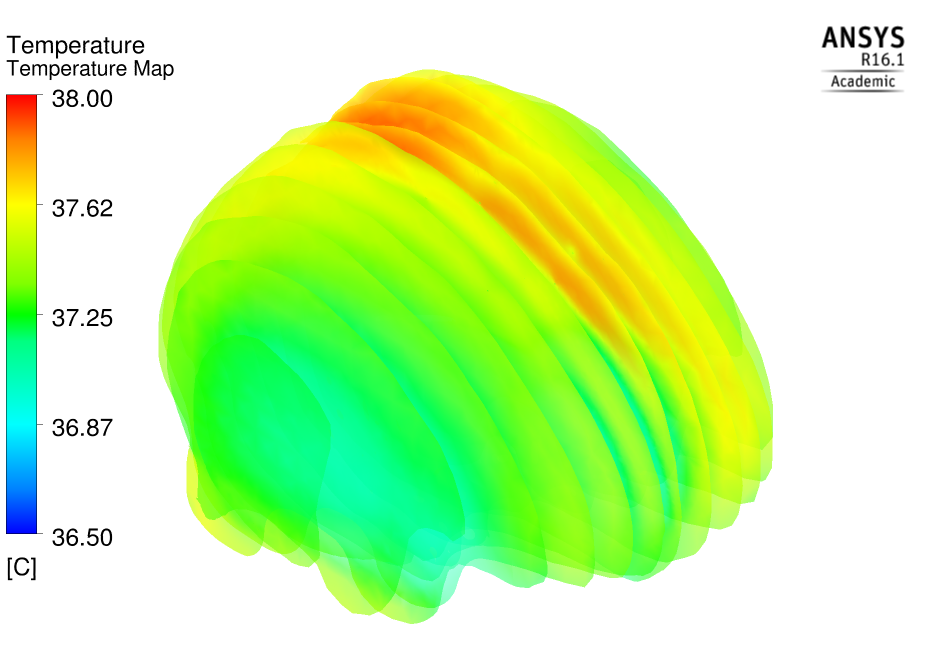
\includegraphics[width=0.6\textwidth]{3DFullVessels/temperatureVolume1}
	\caption[Temperature slices for brain region in sparse arterial tree model, $T_{scalp}=36.5^{o}C$]{Temperature slices for brain region in sparse arterial tree model, $T_{scalp}=36.5^{o}C$.}
	\label{fig:temperatureVolume1}
\end{figure}

Figure.~\ref{fig:temperatureVolume1} shows semi-transparent vertical slices of tissue temperature in the brain domain with a scalp temperature of $36.5^{o}C$. The higher temperatures towards the superior region of the brain match the lack of streamlines observed in Figure~\ref{fig:streamlines1}. Similar to the results in the 3D hemispherical model, the lack of proper distribution of blood leads to regions displaying higher temperatures than expected.

\begin{figure}[h]
	\centering
	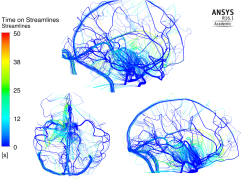
\includegraphics[width=0.7\textwidth]{3DFullVessels/streamlines}
	\caption[1500 flow streamlines generated randomly spread over the inlet areas for the dense arterial tree model]{1500 flow streamlines generated randomly spread over the inlet areas for the dense arterial tree model.}
	\label{fig:streamlines2}
\end{figure}

Figure.~\ref{fig:streamlines2} shows streamlines for the model with dense embedded arterial tree. As before, the streamlines are randomly generated on the inlet surfaces and serve to give an indication of blood flow distribution. The superior region of the brain has more streamlines passing through than with the less dense model. However, there is a dense region of streamlines between the circle of Willis and the sagittal sinus which indicates much of the flow is passing through this region and not distributing evenly. 

\begin{figure}[h]
	\centering
	\begin{subfigure}[b]{0.45\textwidth}
		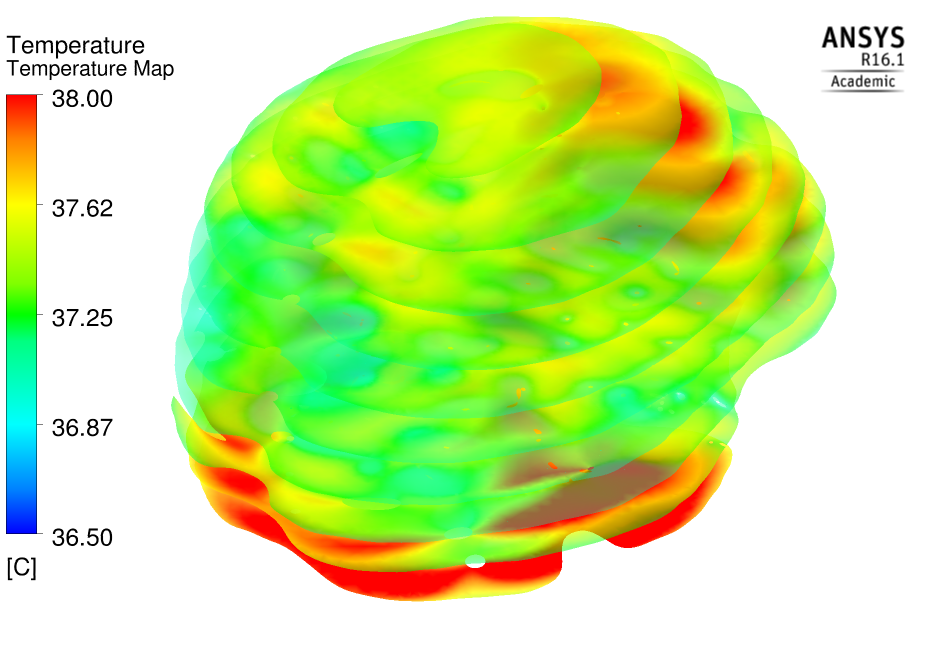
\includegraphics[width=\textwidth]{3DFullVessels/temperatureVolume2a}
	\end{subfigure}
	\begin{subfigure}[b]{0.45\textwidth}
		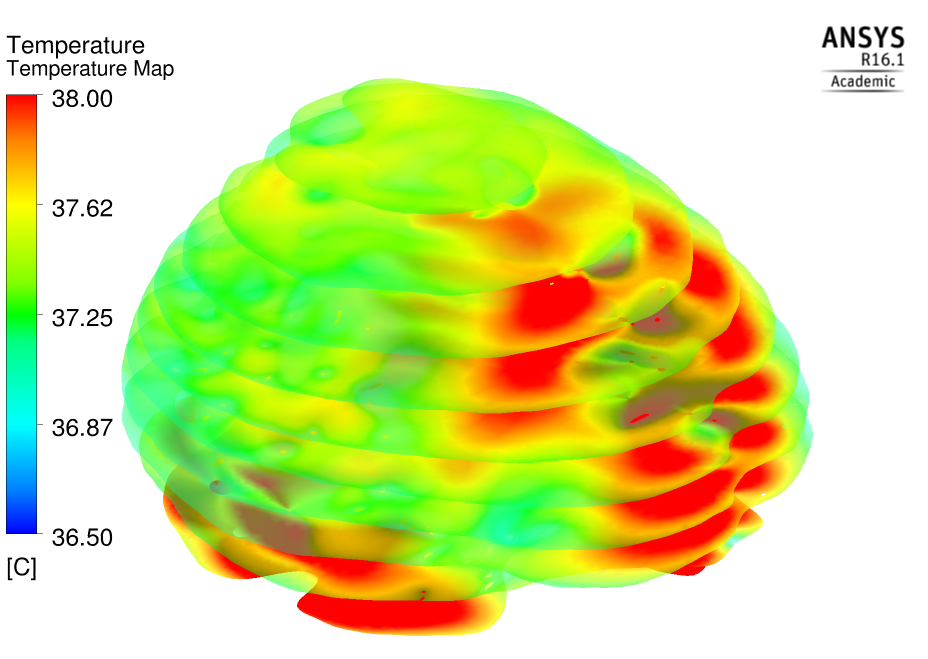
\includegraphics[width=\textwidth]{3DFullVessels/temperatureVolume2b}
	\end{subfigure}
	\caption[Temperature slices for brain region in dense arterial tree model, $T_{scalp}=36.5^{o}C$]{Temperature slices for brain region in dense arterial tree model, $T_{scalp}=36.5^{o}C$.}
	\label{fig:temperatureVolume2}
\end{figure}

This can be further observed in Figure~\ref{fig:temperatureVolume2} whereby the anterior and inferior regions of the brain possess higher temperatures. This shows that, even with the dense arterial tree embedded in the brain, the model does not present an even distribution of blood. This leads to regions of high temperature and poor perfusion which would have a large impact on any investigation of temperature drops. 

\subsection{Conclusion \& Limitations of Method}

The models and results displayed within this chapter are preliminary studies that serve to highlight the difficulties and complications that arise when implementing the directional blood flow into bioheat models. The associated boundary conditions have to generate a flow profile that accurately reflects the distribution of blood within the brain otherwise certain regions display poor perfusion, leading to higher temperatures. 

The simple 1-Dimensional models show that directional flow does have an effect on core brain temperature although this method is limited to exploring radial flow only. In expanding to 3-Dimensional flow, the lack of even distribution of blood prevented any meaningful results from being generated, even with a dense arterial vessel tree. Further expansion of these vessel trees is computationally prohibitive as the smaller branches of the vessel trees would require exponentially smaller voxels to mesh. Additionally, any modification to the created mesh requires a large amount of manual adjustment to ensure the domains are properly segmented. Besides this, grid independence, by refinement of the current mesh, would need to be performed on the presented trials to ensure the validity of the results.

The two main issues with the 3D model are the high voxel density required to simulate a large numbers of complex vessels with small diameters, and controlling the blood flow distribution within the tissue. A solution to complexity of vessel trees is to replace them with 1-Dimensional line segments embedded in the 3D domain, as exhibited by the DiVa model \cite{kotte1996description} and others \cite{d2008coupling,reichold2009vascular}. The blood flow may be controlled with stricter inter-domain parameters or even the introduction of a counter-current flow model. Unfortunately, Ansys CFX does not currently support 1-Dimensional domains, nor does it allow multiple flow domains to be solved within the same space. Therefore, to address these matters, an in-house software was produced which is described in the following chapter. 

\newpage
\thispagestyle{empty}
\chapter[Vascular Porous (VaPor) Model for Temperature and Flow in Cerebral Vasculature and Tissue]{{\Huge V}ascular {\Huge P}orous ({\Huge V}a{\Huge P}or) {\Huge M}odel for {\Huge T}emperature and {\Huge F}low in {\Huge C}erebral {\Huge V}asculature and {\Huge T}issue}
\fancyhead[LE]{\makebox[1cm][r]{\fontfamily{ppl}\thepage\enskip}$\mid$\enskip\makebox[1cm][l]{\fontfamily{ppl}\scriptsize\MakeUppercase{{\small V}ascular {\small P}orous {\small (V}a{\small P}or{\small )} {\small M}odel}}}
\thispagestyle{empty}
\label{Sec:3Chapter3}

\section[Introduction]{{\Large I}ntroduction}
\fancyhead[RO]{\makebox[1cm][r]{\fontfamily{ppl}\small\thesection{ -- }\scriptsize\MakeUppercase{{\small I}ntroduction}}\enskip$\mid$\makebox[1cm][l]{\enskip\fontfamily{ppl}\thepage}}

In the previous chapter, a number of simulations modelling cerebral temperatures were shown with varying degrees of complexity. Using 3-Dimensional blood vessels inside a porous domain proved difficult to manipulate and left many regions under-perfused, affecting the resultant temperatures. This chapter presents the theoretical foundation for the Vascular Porous (VaPor) model developed for this project which replaces the 3-Dimensional vessels with 1-Dimensional segments but maintains the porous media domain separating the arteries and veins. This facilitates control over the distribution of blood throughout the system without resorting to the simplifications posed by the Pennes Bioheat Equation.

The main advantage for using 1-Dimensional line segments to depict the blood vessels is the ease for manipulation and dictating domain transfer. Individual segments within the vessel trees can be isolated to control how much blood is distributed to the porous domain in different regions. Additionally, the trees themselves can be adjusted by adding and removing segments with a few lines of code to determine the effects of vasculature on cerebral temperatures. 

The programming language chosen for the solver was Matlab. This was mainly due to a previous familiarity with the software language. Additionally, it also provides built-in debugging tools and a simple command interface that allows for quick inspection and display of output data. Functions for graph plotting and surface rendering are also included which allow easy and rapid visualisation of profiles produced. Alternative programming languages such as C++ or Fortran could make the software more efficient in terms of optimisation with visualisation being performed using third party software. However, the current model performs well enough and translation to another programming language would take more time than it would probably save. Presently, the typical high-resolution simulation time from start to finish on a laptop with an Intel i5-3340M QuadCore processor and 8GB of RAM is approximately 23 minutes.

The overall procedure for the VaPor model is as follows:

\begin{enumerate}
	\setlength\itemsep{0em}
	\item Obtain data of brain and surrounding tissue to act as 3D domain and discretise into uniform cubic voxels and apply physical values. (Section~\ref{Sec:3Acquiring3dDomains})
	\item Develop arterial and venous trees comprised of 1D segments from existing data or procedurally generate them and place them inside the same space as 3D domain. (Section~\ref{Sec:3AcquiringBloodVesselData})
	\item Establish connections between 1D segments of vessel trees and 3D voxels where they both intersect. (Section~\ref{Sec:3ConnectingVesselsto3dDomain})
	\item Assign which segments deposit and retrieve blood from intersected voxels. (Section~\ref{Sec:3ConnectingVesselsto3dDomain})
	\item Solve flow for 1D segments using vascular resistance model. (Section~\ref{Sec:3Flowrates1d})
	\item Solve flow for 3D capillary region independently from 1D vascular region using mass and momentum equations for porous media. (Section~\ref{Sec:3Flowrates3d})
	\item Assign boundary conditions for heat transfer. (Section~\ref{Sec:3TemperatureSolver})
	\item Solve temperature profiles for both 1D and 3D domains simultaneously using heat transfer equations. (Section~\ref{Sec:3TemperatureSolver})
\end{enumerate}

The following sections describe the VaPor method in detail. For the purpose of clarity, the method is described in the same order as program execution. 

\section[Acquiring 3D Tissue Domains]{{\Large A}cquiring {\Large 3D} {\Large T}issue {\Large D}omains}
\fancyhead[RO]{\makebox[1cm][r]{\fontfamily{ppl}\small\thesection{ -- }\scriptsize\MakeUppercase{{\small A}cquiring {\small 3D} {\small T}issue {\small D}omains}}\enskip$\mid$\makebox[1cm][l]{\enskip\fontfamily{ppl}\thepage}}
\label{Sec:3Acquiring3dDomains}

The head and brain domain data used in this model was extracted from the tissue probability maps provided in the open-source SPM-12 (Statistical Parametric Mapping) \cite{penny2011statistical} (found at \texttt{http://www.fil.ion.ucl.ac.uk/spm/}). This data was then segregated into image stacks which depict the weighted probability of various types of tissue present within the human head. These are both grey and white matter, cerebral spinal fluid (CSF), which include eyeballs, the skull, and miscellaneous soft tissue such as scalp tissue. Each image slice depicts the probability of tissue present in voxels with a value of intensity between zero and one. A representation of the tissue domain is shown in Figure~\ref{fig:TissueDomains}.

\begin{figure}[h]
	\centering
	
	\makebox[0.8\textwidth][c]{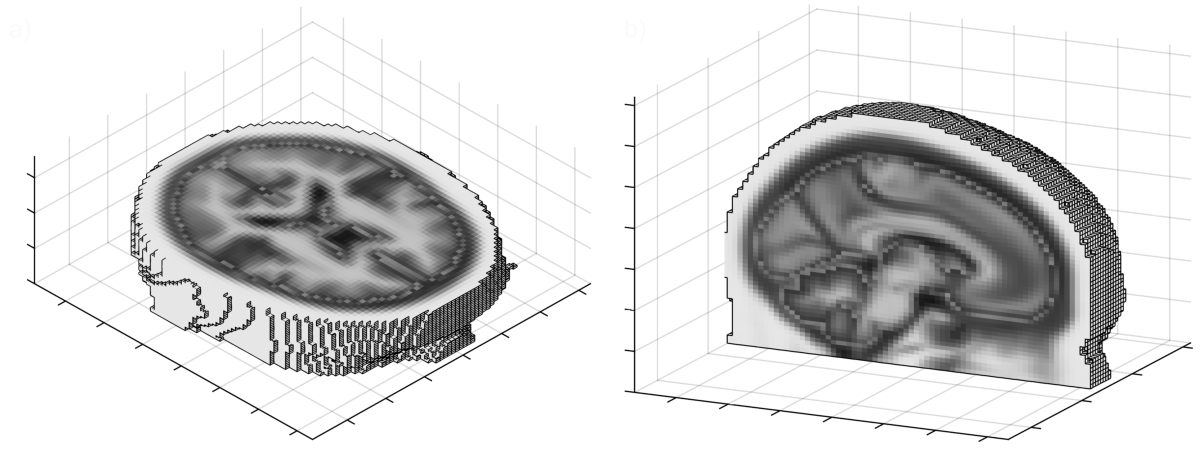
\includegraphics[width=\textwidth]{Chapter3/Figure1}}	
	
	\caption[Slices of head and brain probability maps used for all trials in the VaPor model]{An axial (left) and sagittal (right) slice of the head and brain probability maps used for all trials with the VaPor model. The various tissue types were assigned a shade of grey to highlight the segmentation of the domain.}
	\label{fig:TissueDomains}
\end{figure}

The tissue probability maps are comprised of 5 sets of data, each with 121 image slices of $121\times145$ pixel resolution. This results in a 4-Dimensional $121\times145\times121\times5$ data set. Unfortunately, the machine used for the model does not possess enough memory to handle the linear solver with this large a dataset. It is therefore coarsened to allow various resolutions of the data to be used. A single plane is removed in each dimension (which are all empty) to reduce the size to $120\times144\times120\times5$. This can then be coarsened by averaging data points in a $2\times2\times2$ or a $3\times3\times3$ kernel. The original resolution had each voxel represent a cube of length $1.5mm$, but within the trials, resolutions of $2.25mm$ $3.0mm$, $4.5mm$, and $9.0mm$ are used. Interpolation of data could allow any resolution to be chosen, however, these values were picked as the division always results in a whole number of voxels.

These datasets are imported into the model and then processed slightly in order to create specific cerebral and non-cerebral domains. Voxels which show a combined grey and white matter intensity of greater than $50\%$ of overall combined voxel intensity are considered to be part of the brain, whereas other voxels are not. These cerebral voxels are considered to be only comprised of grey and white matter so the intensities of other tissues in this region are set to zero. Those voxels which are considered non-cerebral have there associated intensities of grey and white matter converted to miscellaneous soft tissue. Physical parameters for tissue are weighted by the intensity levels of the various tissue types in the voxel. Values for physical parameters for each tissue type are given in Table.~\ref{tab:physicalparams2}.

\begin{table}
	\centering
	\fontsize{8pt}{9pt}\selectfont
	\begin{tabular}{l c c l c c}
		\toprule
		\textbf{Physical Parameter} & \textbf{Value} & \textbf{Units} & \textbf{Physical Parameter} & \textbf{Value} & \textbf{Units} \\	
		\hline
		Arterial Blood Temperature, $T_{a}$ & 37$^{\dagger}$ & $^{o}C$ & Perfusion Rate, $\omega$ & & \\
		Blood Viscosity, $\mu_{b}$ & 3.5 & $mPa{\cdot}s$ & \qquad \qquad \qquad Grey Matter & 80$^{\dagger}$ & $ml/100g/min$ \\
		Blood Volume Fraction, $\epsilon_{b}$ & & & \qquad \qquad \qquad White Matter & 20$^{\dagger}$ & $ml/100g/min$ \\
		\qquad \qquad \qquad Grey Matter & 0.0672$^{*}$ & - & \qquad \qquad \qquad CSF & 0$^{\ddagger}$ & $ml/100g/min$ \\
		\qquad \qquad \qquad White Matter & 0.0405$^{*}$ & - & \qquad \qquad \qquad Bone & 1.8$^{\dagger}$ & $ml/100g/min$ \\ 
		Capillary Diameter & 10 & $\mu m$ & \qquad \qquad \qquad Scalp & 2.0$^{\dagger}$ & $ml/100g/min$ \\ 
		Capillary Tortuosity & 2.5 & - & Specific Heat Capacity. $c$  & &\\
		Density, $\rho$ & & & \qquad Tissue & & \\
		\qquad Tissue & & & \qquad \qquad \qquad Grey Matter & 3700$^{\dagger}$ & $J/kg/^{o}C$ \\
		\qquad \qquad \qquad Grey Matter & 1030$^{\dagger}$ & $kg/m^{3}$ & \qquad \qquad \qquad White Matter & 3700$^{\dagger}$ & $J/kg/^{o}C$ \\
		\qquad \qquad \qquad White Matter & 1030$^{\dagger}$ & $kg/m^{3}$ & \qquad \qquad \qquad CSF & 3800$^{\ddagger}$ & $J/kg/^{o}C$ \\
		\qquad \qquad \qquad CSF & 1000$^{\ddagger}$ & $kg/m^{3}$ & \qquad \qquad \qquad Bone & 1590$^{\dagger}$ & $J/kg/^{o}C$ \\
		\qquad \qquad \qquad Bone & 1520$^{\dagger}$ & $kg/m^{3}$ & \qquad \qquad \qquad Scalp & 4000$^{\dagger}$ & $J/kg/^{o}C$ \\
		\qquad \qquad \qquad Scalp & 1000$^{\dagger}$ & $kg/m^{3}$ & \qquad Blood & 3800$^{\dagger}$ & $J/kg/^{o}C$ \\
		\qquad Blood & 1050$^{\dagger}$ & $kg/m^{3}$ & Thermal Conductivity, $K$ & & \\ 
		Metabolic Heat Generation, $Q_{gen}$ &  & & \qquad Tissue & & \\
		\qquad \qquad \qquad Grey Matter & 16700$^{\dagger}$ & $W/m^{3}$ & \qquad \qquad \qquad Grey Matter & 0.49$^{\dagger}$ & $W/m/^{o}C$ \\
		\qquad \qquad \qquad White Matter & 4175$^{\dagger}$ & $W/m^{3}$ & \qquad \qquad \qquad White Matter & 0.49$^{\dagger}$ & $W/m/^{o}C$ \\ 
		\qquad \qquad \qquad CSF & 0$^{\ddagger}$ & $W/m^{3}$ & \qquad \qquad \qquad CSF & 0.5$^{\ddagger}$ & $W/m/^{o}C$ \\ 
		\qquad \qquad \qquad Bone & 368.3$^{\dagger}$ & $W/m^{3}$ & \qquad \qquad \qquad Bone & 1.16$^{\dagger}$ & $W/m/^{o}C$ \\ 
		\qquad \qquad \qquad Scalp & 363.4$^{\dagger}$ & $W/m^{3}$ & \qquad \qquad \qquad Scalp & 0.342$^{\dagger}$ & $W/m/^{o}C$ \\ 
		Nusselt Number, \Nuss & 4 & - & \qquad Blood & 0.492$^{\dagger}$ & $W/m/^{o}C$ \\ \bottomrule
	\end{tabular}
	
	\caption[Physical parameters used in the VaPor model]{Table of physical parameters used in the VaPor model. $^{\dagger}$Values taken from Neimark~\textit{et al.\ }\cite{neimark2008brain}. $^{\ddagger}$Values taken from van~Leeuwen~\textit{et al.\ }\cite{van2000numerical}. $^{*}$Values calculated from cerebral blood volume values given in Larsson~\textit{et al.\ }\cite{larsson2009measurement}.}
	\label{tab:physicalparams2}
\end{table}

Blood flow is modelled within the cerebral voxels only. The surrounding tissue is considered to adhere to Pennes Bioheat Equation. This is mainly due to the lack of information available for non-cerebral head vasculature to properly model the flow. Various aspects of blood flow are therefore omitted that could potentially have an impact on temperature. Heat transfer to the environment occurs only on the scalp and the base of the model connected to the rest of the body is considered to be adiabatic.

\section[Acquiring Blood Vessel Data]{{\Large A}cquiring {\Large B}lood {\Large V}essel {\Large D}ata}
\fancyhead[RO]{\makebox[1cm][r]{\fontfamily{ppl}\small\thesection{ -- }\scriptsize\MakeUppercase{{\small A}cquiring {\small B}lood {\small V}essel {\small D}ata}}\enskip$\mid$\makebox[1cm][l]{\enskip\fontfamily{ppl}\thepage}}
\label{Sec:3AcquiringBloodVesselData}

The vessels within the VaPor model are assumed to be 1-Dimensional line segments with established connectivity. This is the same in practice as in the DiVa model \cite{kotte1999modelling}, however, it differs from previous models in the heat and mass interaction between tissue and vessels. The DiVa model has its own method to generate vasculature, weighted by perfusion \cite{van1998flexible}. Most methods for generating vasculature implement a form of conditional growth algorithm with the diameters of the generated segments relying on established rules to dictate the spread and size of the vessels such as Lindenmayer systems \cite{galarreta2013three}\cite{zamir2001arterial}. These rules are based on accepted trends of vessel growth such as Murray's Law \cite{murray1926physiological} and other scaling laws \cite{francis2009scaling}. 

The VaPor model focusses on delivering blood in a manner that represents the prescribed perfusion values for tissue shown in Table.~\ref{tab:physicalparams2} to avoid regions of poor blood flow that lead to higher than expected temperatures. Therefore, the primary goal of the vessels is to fill the domain volume in a manner proportional to the desired perfusion. To accomplish this, some of the more rigorous aspects of these vessel generation algorithms were foregone in order to proceed with the development of the software. Instead, a simpler space-filling algorithm is used in place of the above methods. One of the simplest methods is utilising a Rapidly-Exploring Random Tree (RRT) algorithm \cite{lavalle1998rapidly}. This process involves procedurally generating points within the volume and connecting them to the nearest point on the previously created vascular tree. Although this does not necessarily adhere to previously established models, it functions to achieve its purpose in generating vessels to distribute blood throughout the domain. 

The RRT algorithm operates as follows: 

\begin{enumerate}
	\setlength\itemsep{0em}
	\item A new node is randomly generated inside the target space domain.
	\item All previous nodes are searched to find the closest segment or node.
	\item A new segment is created by joining the created node to the nearest node, or to the closest point on the nearest segment.
	\item If the new segment is connected to an existing segment (not at a node), a new node is generated on the existing segment, dividing it in two, at the point of intersection.
	\item This is repeated until a specified number of iterations have been completed.
\end{enumerate}

This is repeated for as many times as required. Further conditions can be implemented such as maximising the number of connections that can be on a single node, and adjusting the diameter of vessels as the tree branches out further. Additionally, any previously created vessel structure can be expanded upon using the algorithm without significantly altering the original. Figure~\ref{fig:RRT2D} shows an example of the algorithm operating in a 2D $10\times10$ domain for 5, 10, 100 and 1000 iterations.

\begin{figure}[h]
	\centering
	\makebox[\textwidth][c]{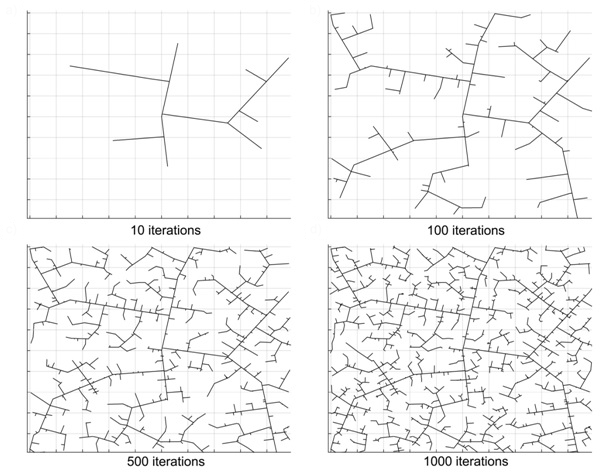
\includegraphics[width=0.6\paperwidth]{Vessels/RRT2D}}
	\caption[RRT algorithm vessel generation for a 2D domain]{RRT algorithm vessel generation for a 2D domain at 10, 100, 500, \& 1000 iterations.}
	\label{fig:RRT2D}
\end{figure}

In the VaPor model, the generation of the new node is spatially weighted by the perfusion term associated with the tissue. Therefore, voxels with higher perfusion (i.e.\ grey matter) have more vessels generated within it and therefore experience more blood flow. This helps ensure a better distribution of blood throughout the domain and prevents regions being disproportionately starved of blood. An example of the weighting is given in Figure.~\ref{fig:RRTComparison}. With the shaded region possessing $4\times$ higher perfusion than the unshaded area, the vessels within the shaded area contain $79.7\%$ of the total lengths of vessels.

\begin{figure}[h]
	\centering
	\makebox[\textwidth][c]{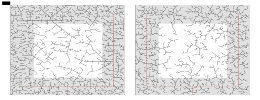
\includegraphics[width=0.6\paperwidth]{Chapter3/RRTComparison}}
	\caption[Comparison of two methods of RRT generation with variable regions of perfusion]{Left: RRT generation for a 2D domain at 2500 iterations. Right: RRT generation with limited segment length for a 2D domain at 2500 iterations. The red segments depict a pre-allocated vessel structure. The shaded area has $4\times$ higher perfusion than the unshaded region and, therefore, attracts $4\times$ number of vessel segments.}
	\label{fig:RRTComparison}
\end{figure}

An additional option can be implemented whereby the length of a segment generated is limited. This gives the vessels a growth-like structure shown in Figure.~\ref{fig:RRTComparison} (right). The newly generated segments have a higher probability of joining on a node termination rather than midway through a segment which leads to more varied bifurcation angles. In performing simulations, both methods give similar results except at low numbers of iterations where the growth-like algorithm does not have time to properly perfuse the domain. To avoid this issue and maintain consistency among trials, this option was not used in simulations and the algorithm from Figure.~\ref{fig:RRTComparison} (left) was used.

The diameters for the generated vessels are supplied from a relationship with mass flowrates \cite{kolios1995large}. The relationship along with corresponding data is shown in Table.~\ref{tab:DtoFlow}.

\begin{table}
	\centering
	\fontsize{8pt}{9pt}\selectfont
	\begin{tabular}{c c c}
		\toprule
		\textbf{Blood Vessel Diameter, $D$ [$mm$]} & \textbf{Average Velocity, $U$ [$cm/s$]} & \textbf{Mass Flowrate, $\dot{F}$ $10^{\smallminus6}kg/s$} \\
		\hline
		2.0 & 20 & 660 \\
		1.4 & 10.5 & 170 \\
		1.0 & 8 & 66 \\
		0.8 & 7.5 & 40 \\
		0.6 & 6.0 & 19 \\
		0.4 & 5.5 & 7.3 \\
		0.2 & 3.4 & 1.1 \\ 
		\multicolumn{3}{c}{Derived Relationship: $D_{v}(\text{m}) = 0.0332*\dot{F}(\text{kg/s})^{0.3703}$} \\ \bottomrule
	\end{tabular}
	\caption[Relationship between blood vessels diameter and velocity]{Relationship between blood vessels diameter and velocity taken from Kolios~\textit{et al.\ }\cite{kolios1995large}. These are converted into mass flowrates and the relationship is given at the base of the table. The units for the variables in the conversion are shown in brackets.}
	\label{tab:DtoFlow}
\end{table}

To supplement the generation of vessels, the dense arterial tree taken from the BraVa database and the venous skeleton extracted from the MRI scan used in the previous chapter were incorporated into the model. This gives a general structure to the randomness of the RRT algorithm. The original vessel trees are shown in Figure.~\ref{fig:RRTfull} alongside the same vessels after 2500 iterations of the RRT algorithm.

\begin{figure}[h]
	\centering
	\begin{subfigure}[b]{0.45\textwidth}
		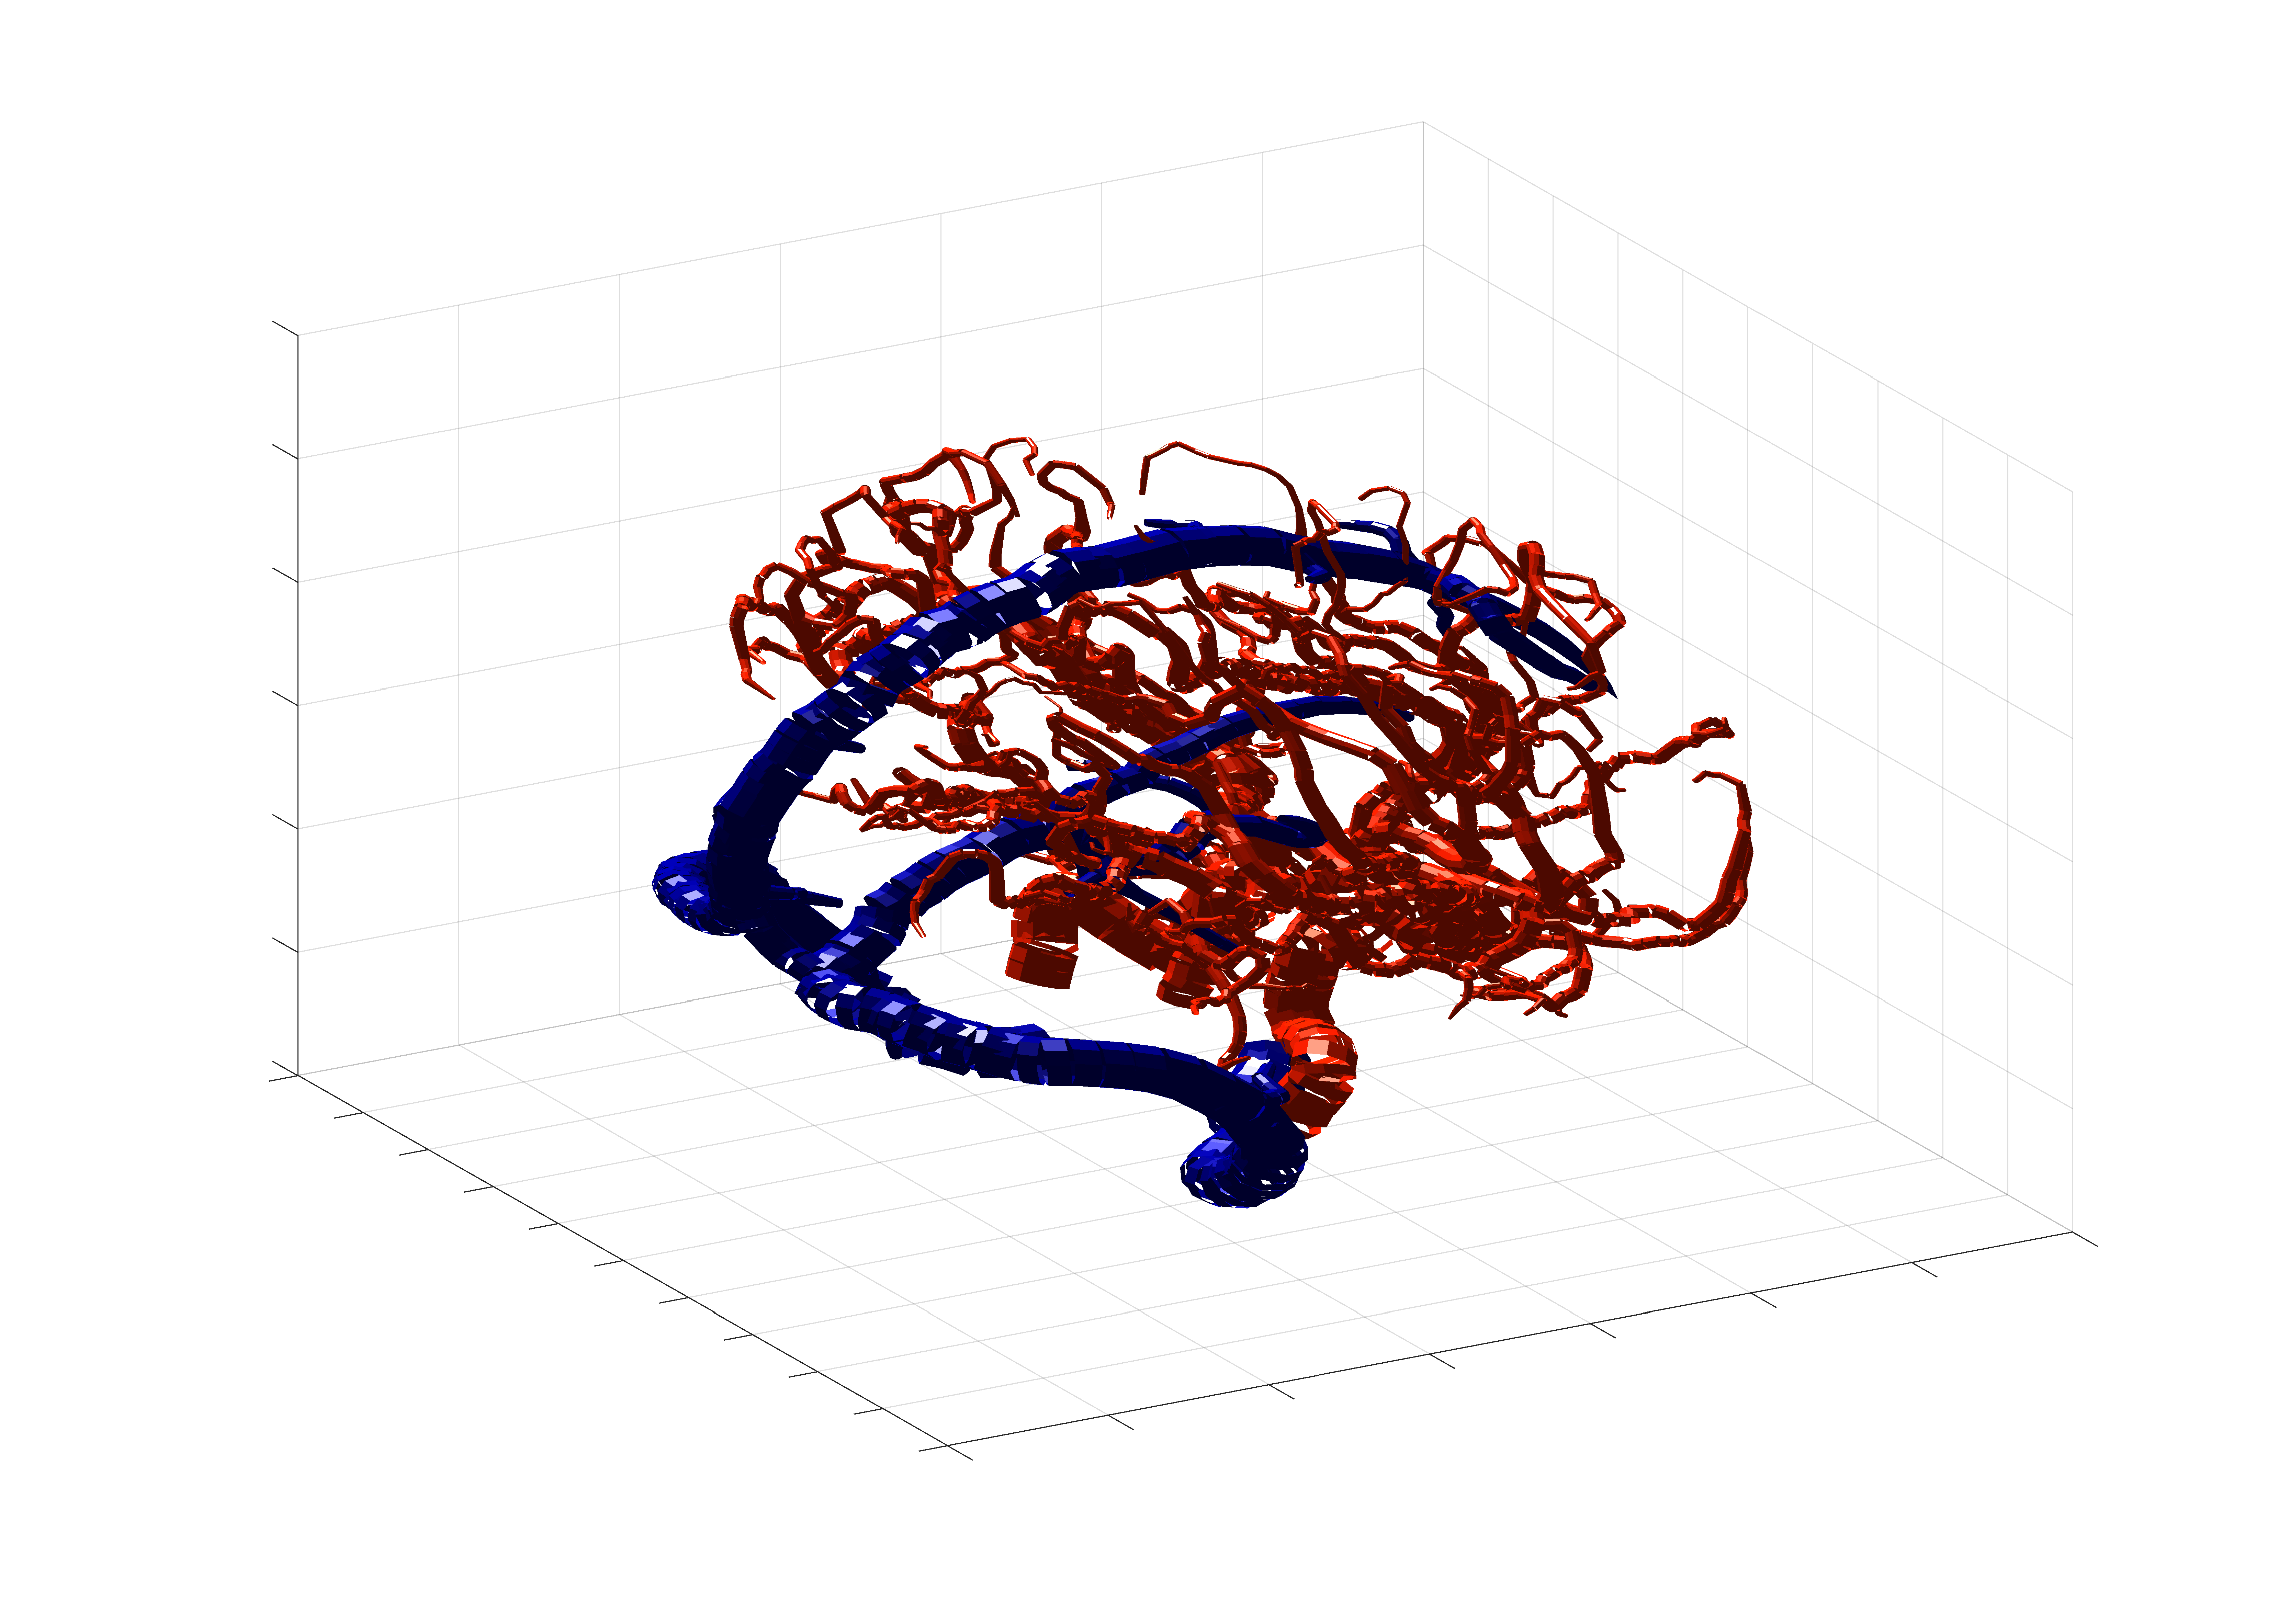
\includegraphics[width=\textwidth]{Chapter3/Chapter3Vessels1}
	\end{subfigure}
	\begin{subfigure}[b]{0.45\textwidth}
		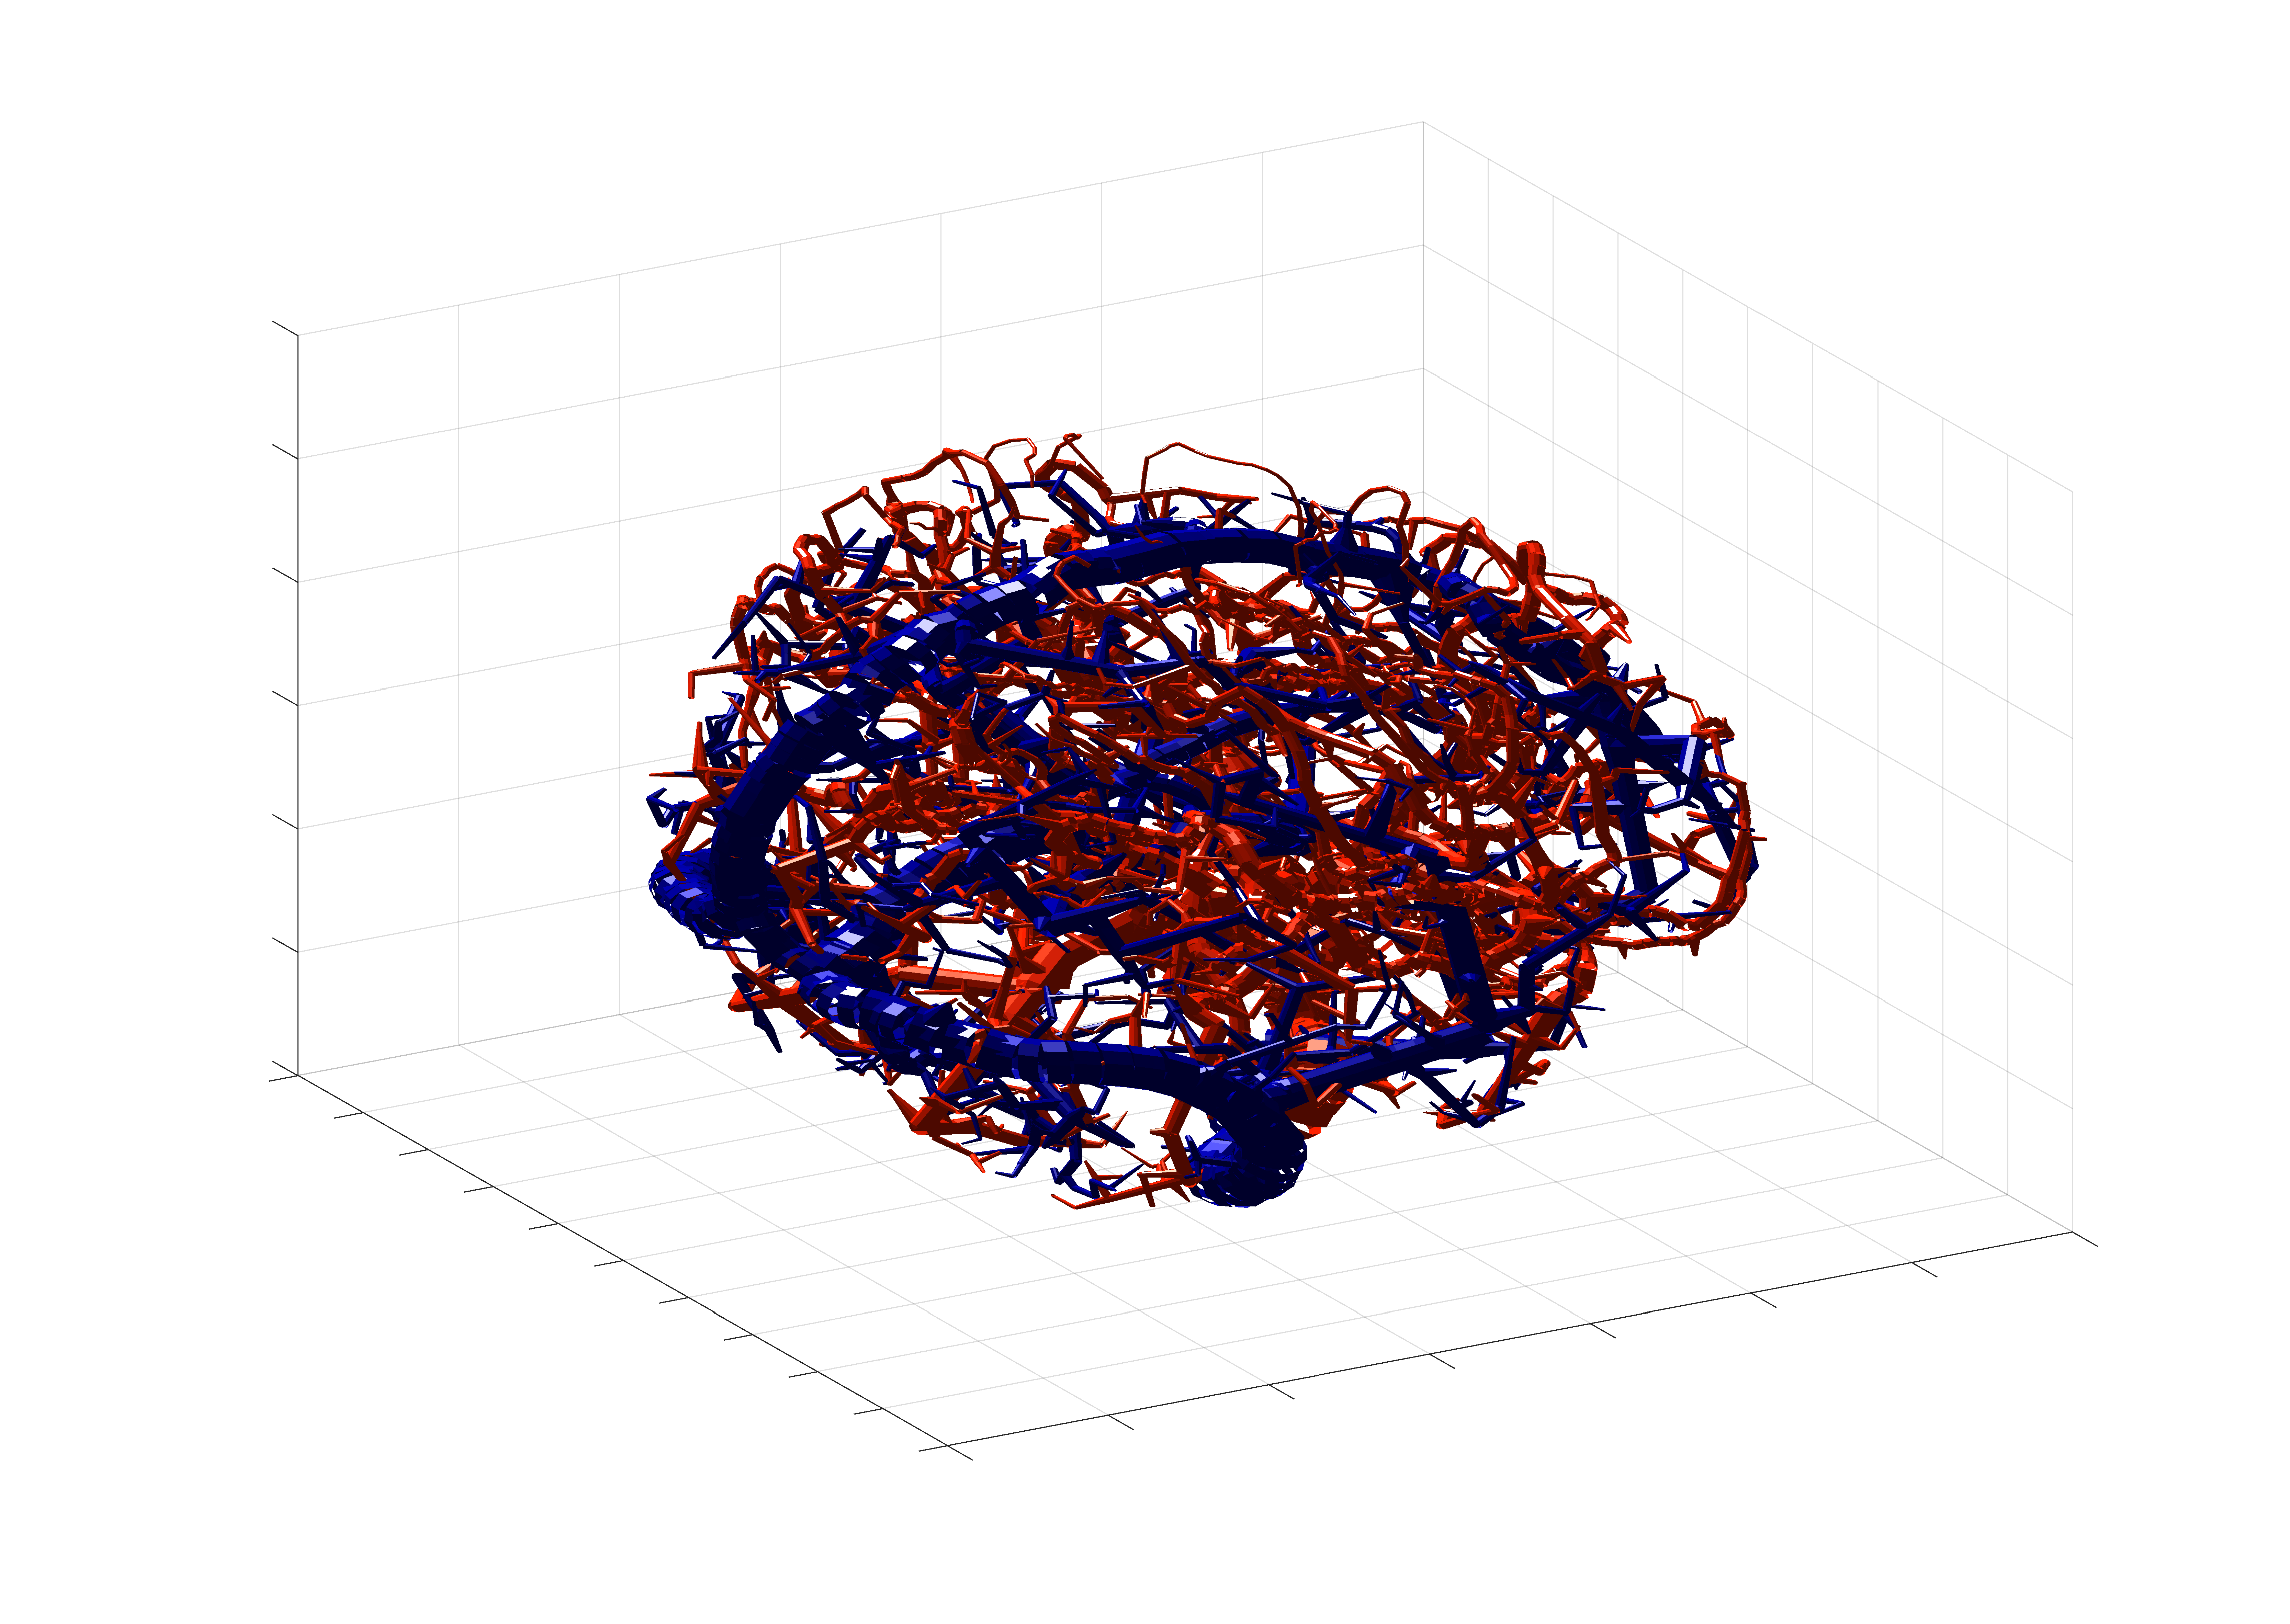
\includegraphics[width=\textwidth]{Chapter3/Chapter3Vessels2}
	\end{subfigure}
	\caption[Vessel expansion using RRT Method and diameters from flow]{Vessel expansion using RRT Method and diameters from flow. Left: original vessel structure. Right: Vessel structure after 2500 iterations of RRT algorithm.}
	\label{fig:RRTfull}
\end{figure}

The vessel geometry is saved in a dataset that contains 7 values for each point. The format is the same as the arterial datasets extracted from BraVa \cite{wright2013digital} and was kept to ensure compatibility with all data in the repository. The values are as follows:

\begin{itemize}
	\setlength\itemsep{0em}
	\item Node Number: Integer value identifying each point.
	\item Classification: Integer representing which vasculature group this node belongs to. This appears in the BraVa data and is used here so that the data matches. The value is unused in the current program.
	\item X-location: Location of node on x-axis.
	\item Y-location: Location of node on y-axis.
	\item Z-location: Location of node on z-axis.
	\item Node Diameter: Diameter of vessel at node (in meters).
	\item Connectivity: Integer value of the Node Number that this node is connected to.
\end{itemize}

\begin{figure}
	
	\begin{subfigure}[c]{0.48\textwidth}
		\centering
		\fontsize{8pt}{9pt}\selectfont
		\begin{tabular}{c c c c c c c c c}
			[ & 1 & 1 & 1.54 & 2.31 & 1.29 & 0.003 & 0 &  \\
			& 2 & 1 & 2.12 & 2.86 & 1.30 & 0.003 & 1 &  \\
			& 3 & 1 & 1.54 & 2.73 & 1.47 & 0.003 & 2 &  \\
			& 4 & 1 & 1.79 & 2.30 & 2.58 & 0.003 & 3 &  \\
			& 5 & 1 & 1.30 & 2.31 & 2.75 & 0.003 & 3 & ] \\
		\end{tabular}
	\end{subfigure} 
	\begin{subfigure}[c]{0.50\textwidth}
		\centering
		\makebox[\textwidth][c]{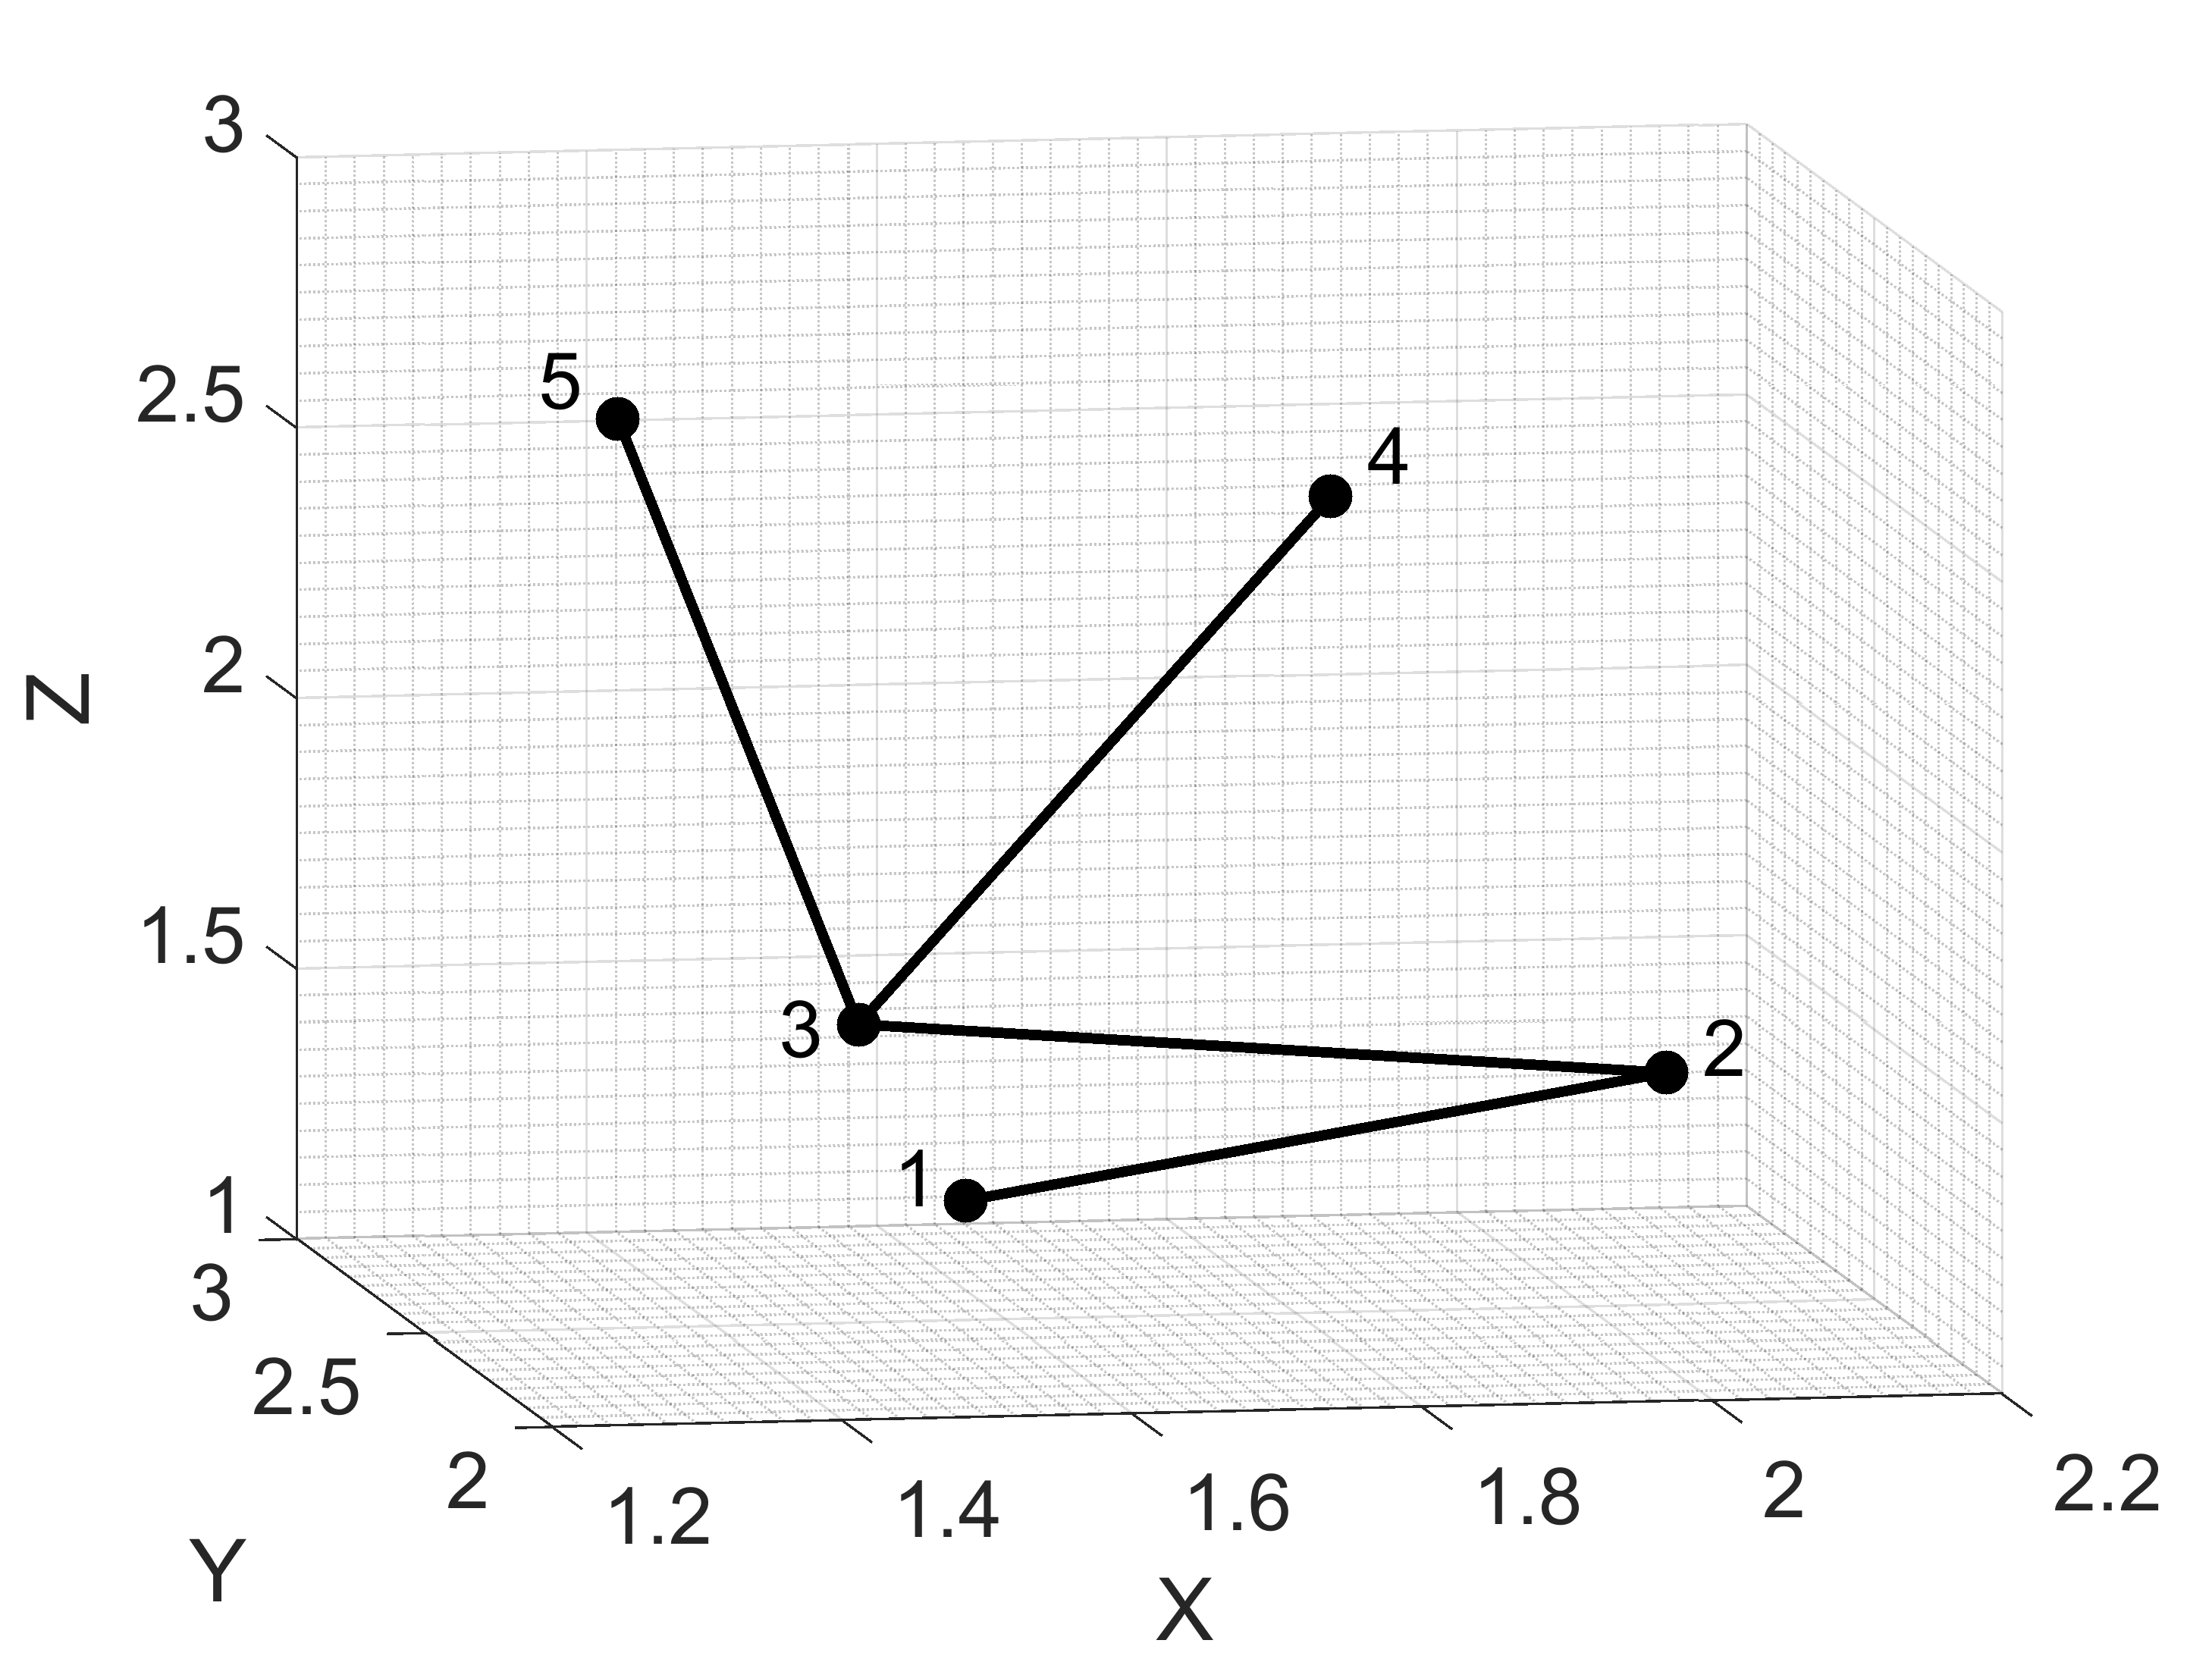
\includegraphics[width=\textwidth]{Vessels/VesselPlot}}		
	\end{subfigure}
	
	\caption[An arbitrary example of a vessel tree dataset with corresponding graphical output]{Left: An arbitrary example of what a vessel tree dataset used in the VaPor model would look like. Right: the corresponding graphical product to the dataset shown. All segments would have diameters of $3mm$.}		
	\label{fig:VesselPlot1}
\end{figure}

The Connectivity for the first node is zero as it is not connected to any other node. An example of a simple data set and the corresponding graphical representation of the data is shown in Figure~\ref{fig:VesselPlot1}.

\section[Connecting Vessels to 3D Domain]{{\Large C}onnecting {\Large V}essels to {\Large 3D} {\Large D}omain}
\fancyhead[RO]{\makebox[1cm][r]{\fontfamily{ppl}\small\thesection{ -- }\scriptsize\MakeUppercase{{\small C}onnecting {\small V}essels to {\small 3D} {\small D}omain}}\enskip$\mid$\makebox[1cm][l]{\enskip\fontfamily{ppl}\thepage}}
\label{Sec:3ConnectingVesselsto3dDomain}

The vessel domains are connected to the 3D voxels by intersection. For the purposes of clarity, the domains are to be named numerically. The 1D arterial vessel tree, the 3D solid tissue phase, the 3D fluid capillary phase and the 1D venous vessel tree are labelled 1, 2, 3, and 4 respectively. A schematic of the model and these domains is shown in Figure~\ref{fig:ExplanationDiagram}. Flow travels in through domain 1 (arteries), passes to domain 3 (capillaries), and then exits through domain 4 (veins). Domain 2 (tissue) is a solid phase, therefore has no flow within it. The tissue and the capillaries (domains 2 \& 3 respectively) occupy the same 3D physical space and function as a porous medium. Each domain is designated a local volume fraction representing the amount of space it takes up within each voxel. Heat transfer occurs between domains 1 and both 2 \& 3, between domains 2 \& 3, and between domains 4 and both 2 \& 3. There is no direct interaction between domains 1 \& 4. 

\begin{figure}[h]
	\centering
	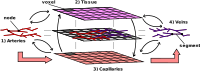
\includegraphics[width=\textwidth]{Chapter3/Chapter3ExplainDrawing}
	\caption[A depiction of the domain structures and interactions present in the VaPor model]{A depiction of the domain structures that the VaPor model uses. The arteries and veins which are 1-Dimensional vessel domains are embedded in a 3-Dimensional domain that is comprised of tissue and capillaries. Heat transfer occurs between all domains except the arteries and veins, as depicted by the thin black arrows. Flow travels from the arteries, to the capillaries, and then to the veins as depicted by the thick red arrows. Additionally, for clarification, the terms `voxel', `node', and `segment' are illustrated here. A `voxel' is a volumetric element of the 3D domains. The shaded examples here all occupy the same space with each domain occupying a certain fraction of the total volume. The `nodes' are points defined by the vessel data sets whereas the `segments' are defined by the connections between `nodes'. Whilst most information is stored at the `nodes', the interaction between domains occurs through the `segments'.}
	\label{fig:ExplanationDiagram}
\end{figure}

Finding the adjacent voxels for each vessel line segment is achieved with a line-cube intersection algorithm. This searches for any intersections between line segments and cube faces. Voxels within the domain sharing this face are added to the list of adjacency for the segment. If none are found then the algorithm checks whether the line segment is located wholly inside a voxel which is then assigned as the neighbour. Otherwise, no adjacency is assigned. All interactions between domains occur between the line segments and their corresponding adjacent voxels.

One of the drawbacks from using this method is associating an interfacial surface area from 1D domains to the 3D domains. Some adjacent voxels would correspond to a larger surface area of the intersecting vessel, however, it is very difficult to calculate these individually. Therefore, all transfer terms between the 1D domains and 3D domains for each segment are independent of location and equally distributed between adjacent voxels. Additionally, the associated diameters of the line segments are ignored when determining neighbours. The diameter of some of the larger arteries and veins may be bigger than the voxels they intersect, meaning a cross-sectional cut of a vessel would occupy more than one voxel. This is ignored for simplicity and the neighbours are only determined by their centreline 1-Dimensional intersection, regardless of the diameter of the vessel.  

Blood flow transfer between the 1D and 3D domains, $\dot{M}$, is weighted by length of vessel segments. For domain 1, blood flow is always out towards domain 3 for domain 4, blood always flows into the vessels from domain 3. All blood flow travels through domain 3 so all branch terminations in domains 1 \& 4 have zero flowrate (except for those designated inlets or outlets).

Temperature information for blood within vessels is stored at each node whereas flow information is stored in the segments. This facilitates maintaining both mass and energy conservation, especially at junctions where the vessels diverge.  

\section[Flow Solvers]{{\Large F}low {\Large S}olvers}
\fancyhead[RO]{\makebox[1cm][r]{\fontfamily{ppl}\small\thesection{ -- }\scriptsize\MakeUppercase{{\small F}low {\small S}olvers}}\enskip$\mid$\makebox[1cm][l]{\enskip\fontfamily{ppl}\thepage}}
\subsection{1-Dimensional Flowrates}
\label{Sec:3Flowrates1d}

\begin{figure}[h]
	\centering
	\begin{subfigure}[b]{0.35\textwidth}
		\centering
		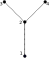
\includegraphics{VesselPoints2}
	\end{subfigure}
	\begin{subfigure}[b]{0.35\textwidth}
		\centering
		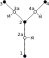
\includegraphics{VesselPoints}
	\end{subfigure}
	\caption[Depiction of additional nodes used in the vessel trees when solving the 1-Dimensional flowrates]{Depiction of an example vessel tree (left), and the additional nodes used in the vessel trees when solving the 1-Dimensional flowrates (right).}
	\label{fig:VesselNodes}
\end{figure}

The equations used to solve flowrate within the vessels are given by:

\begin{equation}
\label{Eq:1DFlowrate}
\sum_1^{n_{1}} G_{1}\Delta P_{1} = -\dot{M}_{1\rightarrow3}
\end{equation}

\begin{equation}
\label{Eq:1DFlowrate2}
\sum_1^{n_{4}} G_{4}\Delta P_{4} = \dot{M}_{3\rightarrow4}
\end{equation}

Where $n_{1}$ and $n_{4}$ represent the number of neighbours of a node or temporary node in domains 1 \& 4 respectively. The subscripts for $\dot{M}$ denote the direction of the exchange and the relative domains. The value, $G$, denotes the conductance of the vasculature and is given by \cite{reichold2009vascular}:

\begin{equation}
\label{Eq:1DConductance}
G_{1} = \frac{\rho_{b}\pi {D_{1}}^{4}}{128\mu_{b}L_{1}}
\end{equation}

\begin{equation}
\label{Eq:1DConductance2}
G_{4} = \frac{\rho_{b}\pi {D_{4}}^{4}}{128\mu_{b}L_{4}}
\end{equation}

Where $L$ is the length of a vessel segment. In the solver, having $\dot{M}$ occur at the nodes can become confusing and confounded with nodes that are inlets or outlets. Instead, the inter-domain transfer is designated to occur between nodes. To account for this in the model, extra nodes are temporarily added as shown in Figure~\ref{fig:VesselNodes}. Nodes that are designated inlets or outlets have a source term added to that node (not the temporary node) to represent blood travelling in or out of the domain.

All branch terminations are assumed to have zero flow as the inter-domain mass transfer is set to equal the overall flow of the system. Therefore, wall boundary conditions are set at these point where the pressure on the node equals the pressure at the temporary node in the segment. Additionally, a single branch termination is designated $P=0$ so that the system is fully bounded. As pressure is unused after this stage and is not applied across domain boundaries, this arbitrary assignment has no effect on the results. It only serves to allow the solving for $\Delta P$.

From Equation~\ref{tab:DtoFlow}, the vessel diameters are dependant on flowrate, however, the vessel diameters are required in Equations.~\ref{Eq:1DConductance}~\&~\ref{Eq:1DConductance2} to solve for flowrate. Therefore, the process for calculating flowrates in domains 1 \& 4 have to be iterated until the diameters converge (residual tolerance is average difference of $10^{\smallminus10}m$). 

Inlet flowrates for the arteries were split 40\%, 40\%, 20\% of the overall flow between the left and right internal carotid arteries and basilar artery respectively \cite{tanaka2006relationship}. The outlet flowrates in the veins were also set and split equally between the two transverse sinuses. While a pressure boundary could be used at vessel terminations in order to naturally solve for outlet flowrates, this method facilitates the calculation of vessel diameters. Adjusting the distribution of flow at the outlets to favour one side or the other has negligible effects on the results. As all inlet and outlet flowrates are set, convergence of diameters occurs immediately as the flow profile is predominantly set. If pressure boundary conditions were used instead, the iteration would take longer.   

Once the pressures have been solved, the mass flowrates and velocities can be calculated using:

\begin{equation}
\label{Eq:1DVelocities}
\dot{F}_{1}=\rho_{b}\frac{\pi {D_{1}}^{2}}{4}U_{1} = G_{1}\Delta P_{1}
\end{equation}

\begin{equation}
\label{Eq:1DVelocities2}
\dot{F}_{4}=\rho_{b}\frac{\pi {D_{4}}^{2}}{4}U_{4} = G_{4}\Delta P_{4}
\end{equation}

Due to the temporary nodes, each line segment ends up with two set of flowrates: one before $\dot{M}$ occurs and one after. Convention dictates that for a line segment defined by node $n$, a positive velocity indicates flow towards node $n$ and a negative value indicates flow away from node $n$. Some segments contain two flowrates with opposite directions. These are considered `split' flow and are treated slightly differently when resolving temperature interactions.

\subsection{3-Dimensional Flowrates}
\label{Sec:3Flowrates3d}

Originally, the VaPor model used a SIMPLE (Semi-Implicit Method for Pressure Linked Equations) algorithm \cite{ferziger1997computational} to solve for velocities with an inertial sink due to the porous nature of capillaries. However, due to the high levels of dampening from this sink, the model became unstable at low values for porosity. Instead, it was shown that adopting Stoke's Regime \cite{holdich2002fundamentals} made negligible difference to the results. As there are no inertial effects in Stoke's Regime, the flowrates are entirely pressure driven and can be solved in a similar manner to the vasculature regions.

For porous media and Stoke's Regime, pressure within each voxel can be solved using a similar resistance model to the 1-Dimensional domains \cite{holdich2002fundamentals}: 

\begin{equation}
\label{Eq:3DFlowrate}
\sum_1^{n_{3}} G_{3}\Delta P_{3} = \dot{M}_{1\rightarrow3}-\dot{M}_{3\rightarrow4}
\end{equation}

Where $n_{3}$ represents the number of neighbours of a voxel in domain 3 which are not beyond a wall boundary. The mass flowrates and velocities between voxels can then be calculated using:

\begin{equation}
\label{Eq:3DVelocities}
\dot{F}_{3}=\rho_{b}l^{2}U_{3} = G_{3}\Delta P_{3}
\end{equation}

The vascular conductance, $G_{3}$, derived using the same theory behind the derivation of the Carmen-Kozeny equation for porous media. The blood flow is assumed to be transported through a number of thin tortuous tubes. The superficial velocity, $U_{3}$, is then related to the actual velocity $U_{3}'$ by:

\begin{equation}
U_{3}' = U_{3}\frac{\tau}{\epsilon_{3}}
\end{equation}

Where $\tau$ is the tortuosity of the capillary vessels which is defined as the ratio of distance travelled by fluid to the distance between the two end points of the path. If this is inserted into the Hagen-Poiseuille equation \cite{white2003fluid}, the resultant equation is formed:

\begin{equation}
\frac{\Delta P}{l} = \frac{32\mu_{b}\tau}{{D_{c}}^{2}\epsilon_{3}}U_{3}
\end{equation}

Converting the velocity to a mass flowrate between voxels gives:

\begin{equation}
\frac{\Delta P}{l} = \frac{32\mu_{b}\tau}{{D_{c}}^{2}\epsilon_{3}}\frac{\dot{F}_{3}}{l^{2}\rho_{b}}
\end{equation}

And then after rearranging to the same form as Equations~\ref{Eq:3DVelocities} the value for vascular conductance can be found to be:

\begin{equation}
\label{Eq:3DConductance}
G_{3} = \frac{\rho_{b}\overline{\epsilon}_{3}l\pi {D_{c}}^{2}}{32\mu_{b}\tau}
\end{equation}

The value, $\overline{\epsilon}_{3}$, represents the average of the porosities in current and adjacent voxels. The values for capillary diameter and tortuosity were assumed to be constant throughout and were designated values of $10\mu m$ and $2.5$ respectively.

There is no velocity perpendicular to wall boundaries but there is also no frictional resistance tangential to the walls (free-slip flow). There are no other boundary conditions except for the domain mass transfer (i.e.\ no other inlets or outlets). 

\section[Temperature Solver]{{\Large T}emperature {\Large S}olver}
\fancyhead[RO]{\makebox[1cm][r]{\fontfamily{ppl}\small\thesection{ -- }\scriptsize\MakeUppercase{{\small T}emperature {\small S}olver}}\enskip$\mid$\makebox[1cm][l]{\enskip\fontfamily{ppl}\thepage}}
\label{Sec:3TemperatureSolver}
The temperature equations for each domain are given below:

\begin{equation}
\label{Eq:Thermal1}
V_{1}\rho_{b}c_{b}\frac{\partial T_{1}}{\partial t}=V_{1}K_{b}(\nabla^{2}T_{1})-V_{1}\rho_{b}c_{b}U_{1}(\nabla T_{1})+\beta_{1\leftrightarrow2}(T_{2}-T_{1})+\beta_{1\leftrightarrow3}(T_{3}-T_{1})
\end{equation}
\begin{multline}
\label{Eq:Thermal2}
V_{2}\epsilon_{2}\rho c\frac{\partial T_{2}}{\partial t}=V_{2}\epsilon_{2} K(\nabla^{2}T_{2})-\beta_{1\leftrightarrow2}(T_{2}-T_{1})+\beta_{2\leftrightarrow3}(T_{3}-T_{2})+\\
\beta_{2\leftrightarrow4}(T_{4}-T_{2})+V_{2}Q_{gen}
\end{multline}
\begin{multline}
\label{Eq:Thermal3}
V_{3}\epsilon_{3}\rho_{b}c_{b}\frac{\partial T_{3}}{\partial t}=V_{3}\epsilon_{3}K_{b}(\nabla^{2}T_{3})-V_{3}\rho_{b}c_{b}U_{3}(\nabla T_{3})-\beta_{1\leftrightarrow3}(T_{3}-T_{1})-\\\beta_{2\leftrightarrow3}(T_{3}-T_{2})
+\beta_{3\leftrightarrow4}(T_{4}-T_{3})+c_{b}\dot{M}_{1\rightarrow3}(T_{3}-T_{1})
\end{multline}
\begin{multline}
\label{Eq:Thermal4}
V_{4}\rho_{b}c_{b}\frac{\partial T_{4}}{\partial t}=V_{4}K_{b}(\nabla^{2}T_{4})-V_{4}\rho_{b}c_{b}U_{4}(\nabla T_{4})-\beta_{2\leftrightarrow4}(T_{4}-T_{2})-\\
\beta_{3\leftrightarrow4}(T_{4}-T_{3})+c_{b}\dot{M}_{3\rightarrow4}(T_{4}-T_{3})
\end{multline}

Where $V$ is the volume of voxel or segment within the domain shown in the subscript and the term $\beta$ denotes a domain heat transfer coefficient for the two domains expressed in the subscript. For tissue that is present in the model, but is not considered within the cerebral domain (for instance, surrounding CSF, skull tissue or scalp tissue), the original Pennes Bioheat Equation is implemented for simplicity. This prevents the need for additional vascular information for the surrounding tissue. These regions are considered to be part of domain 2 but with a volume fraction $\epsilon_{2}=1$ meaning there is no blood phase in this region. However, there may still be intersections with domains 1 \& 4 and corresponding heat transfer occurs in these intersections. The temperature equation for this region is then given by:

\begin{equation}
\label{Eq:Thermal5}
V_{2}\rho c\frac{\partial T_{2}}{\partial t}=V_{2}K(\nabla^{2}T_{2})-\beta_{1\leftrightarrow2}(T_{2}-T_{1})+\beta_{2\leftrightarrow4}(T_{4}-T_{2})+V_{2}c_{b}\frac{\rho}{\rho_{b}}\omega(T_{2}-T{a})+V_{2}Q_{gen}
\end{equation}

The solver relies on the fact that Equations~\ref{Eq:Thermal1}~-~\ref{Eq:Thermal5} can be written as a sum of energy transfers of varying forms into and out of a volume. All physical properties are considered independent of temperature within the expected ranges. Therefore, a linear set of equations can be developed dependant on thermal driving forces.

For a steady-state system, all $\partial T / \partial t$ terms reduce to 0. Therefore, the sum of all energy transfer terms have to equal 0 and can be written as:

\begin{equation}
\label{Eq:TempSum}
0 = \sum Q_{X}
\end{equation}

Where $X$ denotes a type of energy transfer and the units of $Q_{X}$ are in watts. The different types of $X$ are given in Table.~\ref{tab:EnergyTransfer}.

\begin{table}[h]
	\centering
	\fontsize{8pt}{9pt}\selectfont
	\begin{tabular}{c p{6.5cm}}
		\toprule
		$\mathbf{Q_{X}}$ & \textbf{Description}\\ \hline
		$Q_{C}$ & Conduction \\  
		$Q_{V}$ & Convection \\ 
		$Q_{I}$ & Inter-domain heat conduction \\ 
		$Q_{M}$ & Inter-domain heat convection from blood transfer\\ 
		$Q_{G}$ & Metabolic heat generation \\ 
		$Q_{Pen}$ & Heat transfer using Pennes Bioheat Equation \\ \bottomrule
	\end{tabular}
	\caption[Index for the various types of heat transfer that occur in the VaPor model]{Index for the various types of heat transfer that occur in the VaPor model.}
	\label{tab:EnergyTransfer}
\end{table}

The various forms of heat transfer are explained in more detail below. The subscripts $i,j,k$ denote the location of a local value in the 3-Dimensional domain (domains 2 \& 3). The subscript $v$ denotes the location of a local value at a specific node in a 1-Dimensional domain (domain 1 or 4). For each $v$ (except $v=1$) there is an associated segment defined by its single connection. Properties associated with the segment (such as inter-domain heat and mass transfer) are also saved at the location $v$. The subscripts $adj$ and $v,adj$ are used to express a single adjacent connected partner to a voxel or vessel node respectively.

\subsection{Conduction}

\subsubsection{Porous Media (Domains 2 \& 3)}

The conductive heat transfer term using central-differencing discretisation for all sides of a voxel can be written as:

\begin{equation}
\label{Eq:Conduction2}
Q_{Ci,j,k}=A\epsilon_{i,j,k}K_{i,j,k} \sum_{adj=1}^{n}\bigg(\frac{T_{adj}-T_{i,j,k}}{l}\bigg)
\end{equation}

Where $n$ here denotes the number adjacent or neighbouring voxels. For domain 2, the physical parameters $\epsilon$ and $K$, vary locally due to tissue composition. Therefore, they are designated local values (hence the subscript $i,j,k$). For domain 3, the volume fraction varies locally (given by $\epsilon_{3}=1-\epsilon_{2}$) but the thermal conductivity ($K_{b}$) remains constant. As the domain is entirely cubic, the area of a voxel, $A$, is given by the voxel length, $l$, squared ($A=l^{2}$).

\subsubsection{Boundary Conditions}

If the voxel in question lies on a boundary, then one or more of its faces has a boundary condition implemented instead of conductive heat transfer. This is given in the form of:

\begin{equation}
\label{Eq:Boundary}
Q_{Ci,j,k}=A\epsilon_{i,j,k}h_{out}(T_{out}-T_{i,j,k})
\end{equation}

where $h_{out}$ is the surface heat transfer coefficient and $T_{out}$ is the outside temperature.

At the base of the model, the boundary is considered to be adiabatic and therefore $h_{out}=0W/m^{2}/^{o}C$. Otherwise the typical heat transfer coefficient for skin is assumed to be $h_{out}=4W/m^{2}/^{o}C$ \cite{nelson1998brain}. Additionally, a boundary temperature can be set by setting $h_{out}\rightarrow\infty$ which, within the model, sets the boundary condition to $T_{i,j,k}=T_{out}$ instead. This is used to specify a desired scalp temperature, $T_{scalp}$, within the results produced.

The overall conduction for porous tissue can then be written as:

\begin{equation}
Q_{Ci,j,k}=\sum_{adj=1}^{n}
\begin{cases}
A\epsilon_{i,j,k}h_{out}(T_{out}-T_{i,j,k}) & \text{when $adj$ is beyond a boundary} \\
A\epsilon_{i,j,k} K_{i,j,k}\big(\frac{T_{adj}-T_{i,j,k}}{l}\big) & \text{when $adj$ is not beyond a boundary}
\end{cases}
\end{equation}

\subsubsection{Vessels (Domains 1 \& 4)}

The conduction between two nodes in the vessel tree is performed using the length of the segment and the average cross sectional area. The diameters of segments are saved at the nodes and are assumed to vary linearly across the segment length. Therefore, the average cross sectional area, $A_{Xsec}$, is given by:

\begin{equation}
A_{Xsec} = \frac{1}{12}\pi({D_{v}}^2 + {D_{adj}}^2+D_{v}D_{adj})
\label{Eq:CrossSectionArea}
\end{equation}

The conduction heat flux between two vessel nodes is then given by:

\begin{equation}
Q_{Cv}=K_{b}A_{Xsec}\frac{T_{v,adj}-T_{v}}{L_{v}}
\end{equation}

And the overall vessel conduction for a single node can be written as:

\begin{equation}
Q_{Cv}=\sum_{v,adj=1}^{n}K_{b}A_{Xsec}\frac{T_{v,adj}-T_{v}}{L_{v}}
\end{equation}

Where $n$ represents the number of connections present for a node.

\subsubsection{Boundary Conditions}

There is no conductive heat transfer at the boundaries for domains 1 \& 4 meaning at branch terminations:

\begin{equation}
\frac{\partial T_{v}}{\partial L} = 0
\end{equation}

\subsection{Convection}

\subsubsection{Porous Media (Domains 2 \& 3)}

There is no convection present in domain 2. For domain 3, the convective terms are solved on an upstream basis. Flow moving away from the volume has no physical effect on the temperature in that volume. Therefore, only upstream velocities are considered.

\begin{equation}
Q_{Vi,j,k}=\sum_{adj=1}^{n}
\begin{cases}
\lvert U_{adj}\rvert A\rho_{b}c_{b}(T_{adj}-T_{i,j,k}) & \text{when $U_{adj}\cdot \mathcal{N}_{adj} < 0$} \\
0 & \text{when $U_{adj}\cdot \mathcal{N}_{adj} \geq 0$}
\end{cases}
\label{Eq:3DConvection}
\end{equation}

where $U_{adj}$ is the tangential velocity between the two volumes and $\mathcal{N}_{adj}$ is a directional vector towards the adjacent element. If the direction and velocity are opposite directions then the product will be negative and there is flow entering the volume. 

\subsubsection{Boundary Conditions}

Velocities at domain boundaries are already set to zero. No additional boundary conditions are given for convective heat transfer in domain 3.

\subsubsection{Vessels (Domains 1 \& 4)}

Convection within vessels is performed similarly to the convection in the three dimensional domain. However, the flowrate within vessels is saved as a mass flowrate instead of a velocity. Therefore, the heat transfer from convection is given by:

\begin{equation}
Q_{Vv}=\sum_{v,adj=1}^{n}
\begin{cases}
\lvert \dot{F}_{v,adj}\rvert c_{b}(T_{v,adj}-T_{v}) & \text{when $\dot{F}_{v,adj}\cdot \mathcal{N}_{v,adj} < 0$} \\
0 & \text{when $\dot{F}_{v,adj}\cdot \mathcal{N}_{v,adj} \geq 0$}
\end{cases}
\end{equation}

\subsubsection{Boundary Conditions}

For domain 1, arterial inlets are defined. An additional heat transfer is then performed for the inlet flowrates:

\begin{equation}
Q_{Vv}=\dot{F}_{inlet}c_{b}(T_{a}-T_{v})
\end{equation}

\subsection{Inter-Domain Heat Transfer}
\subsubsection{Porous Media (Domains 2 \& 3)}

The inter-phase heat transfer between domains 2 \& 3 are given by the terms:

\begin{equation}
\begin{split}
Q_{Ii,j,k} &= \beta_{2\leftrightarrow3}(T_{3}-T_{2}) \text{\quad for domain 2} \\
Q_{Ii,j,k} &= -\beta_{2\leftrightarrow3}(T_{3}-T_{2}) \text{\quad for domain 3} \\
\end{split}
\end{equation} 

In this case, $\beta$, is a condensed form of $h_{bt}\alpha_{bt}$ present in the Porous Two Phase model and Counter-Current model in Section~\ref{Sec:21DHemisphereTheory}, multiplied by the voxel volume, $V$. As this porous domain is meant to represent the capillaries within the tissue, inter-phase heat transfer is expected to be very high. Therefore, the value for $\beta_{2\leftrightarrow3}$ is expected to be very high. Within the model it is assumed that $\beta_{2\leftrightarrow3}\rightarrow\infty$ which means $T_{3}=T_{2}$. This facilitates solving as it means only a single temperature needs to be solved for the 3-Dimensional domain. This can be implemented by summing up the heat transfer types, $Q_{X}$, from domains 2 \& 3 together in Equation~\ref{Eq:TempSum}. Alternatively, a temperature driving force can be set by using a finite value for $\beta_{2\leftrightarrow3}$ and $T_{2}$ and $T_{3}$ will be two separate values.

\subsubsection{Transfer between 1D (domains 1 \& 4) and 3D (domains 2 \& 3)}

The theory for heat transfer between vessels and the porous media is assumed to be very similar to laminar flow in a rigid pipe. This is governed by the Nusselt number which represents the ratio of heat transfer at the surface of the pipe to the heat transfer of the fluid within the pipe. 

\begin{equation}  
\Nuss = \frac{hD_{v}}{2K_{b}} 
\end{equation}

It has been well established that for laminar flow in a pipe $\Nuss=4$ \cite{bergman2011fundamentals}. Due to the shear-thinning properties of blood, this value may be slightly higher in the larger vessels, however, this has been omitted for simplicity.

As the diameter varies along the length of a vessel segment, $D_{v}$ is replaced with the average diameter $\frac{1}{2}(D_{adj}+D_{v})$. The heat transfer is given by:

\begin{equation}
\label{Eq:InterDomain}
Q_{I}=\pm\sum_{1}^{m}\beta_{x\leftrightarrow y}(T_{v}-T_{i,j,k})/m
\end{equation}

Where $m$ represents the number of voxels intersected by the vessel segment, $x$ \& $y$ represent domain pairs 1 \& 2, 1 \& 3, 2 \& 4, or 3 \& 4, and: 

\begin{equation}
\beta_{x\leftrightarrow y} = \epsilon hA_{surf} 
\end{equation}

with: 

\begin{equation}  
h = \Nuss\frac{4K_{b}}{D_{adj}+D_{v}}
\end{equation}

The inter domain surface area of the segment is given by:

\begin{equation}  
A_{surf} = \pi\frac{D_{adj}+D_{v}}{2}\sqrt{\Big(\frac{D_{adj}}{2}-\frac{D_{v}}{2}\Big)^{2}+{L_{v}}^{2}}
\end{equation}

When dealing with the intersection of vessels and voxels, the transfer between the two is divided equally between the number of intersected voxels, $m$. The transfer is independent of the length of intersection or projected surface area between voxel and line segment. This is to avoid complexities with associated surface areas.

Additionally, the heat transfer for a pipe should be affected as the temperature rises. A true representation of the temperature driving force would be a log mean temperature difference between two points in the segment. This non-linearity cannot be implemented into the linear solver but the average of temperatures is used as an approximation instead. This makes Equation~\ref{Eq:InterDomain} become:

\begin{equation}
\label{Eq:InterDomain2}
Q_{I}=\pm\sum_{1}^{m}\bigg(\frac{1}{2}\beta_{x\leftrightarrow y}(T_{v}-T_{i,j,k})/m+\frac{1}{2}\beta_{x\leftrightarrow y}(T_{v,adj}-T_{i,j,k})/m\bigg)
\end{equation}

Within domains 1 \& 4, this heat transfer is only applied to downstream nodes in vessel segments. This is because the transfer of heat only occurs as the blood is flowing through the segment. Therefore, a condition is added whereby:

\begin{equation}
Q_{I}=\pm\sum_{1}^{m}
\begin{cases}
\!\begin{aligned}%[b]
& \frac{1}{2}\beta_{x\leftrightarrow y}(T_{v}-T_{i,j,k})/m \\
& +\frac{1}{2}\beta_{x\leftrightarrow y}(T_{v,adj}-T_{i,j,k})/m
\end{aligned}           & \text{when $\dot{F}_{v,adj}\cdot \mathcal{N}_{v,adj} < 0$} \\
\\
\qquad \qquad \quad 0 & \text{when $\dot{F}_{v,adj}\cdot \mathcal{N}_{v,adj} \geq 0$}
\end{cases}
\end{equation}

\subsection{Inter-Domain Heat Convection from Blood Transfer}

\subsubsection{Transfer from domain 1 to domain 3}

As above with the inter-domain heat transfer, the distribution of blood from domain 1 to domain 3 occurs equally between the $m$ voxels that intersect the vessel line segment. So for convective heat transfer from domain 1 (arteries) and domain 3 (voxels) the heat transfer is given by:

\begin{equation}
Q_{Mi,j,k}=c_{b}\dot{M}_{1\rightarrow3}(T_{1}-T_{3})/m
\end{equation}

\subsubsection{Transfer from domain 3 to domain 4}

Similarly, the transfer of blood from domain 3 (voxels) to domain 4 (veins) is divided up between the $m$ voxels that intersect the vessel line segment. So for convective heat transfer from domain 3 (voxels) and domain 4 (veins) the heat transfer is given by:

\begin{equation}
Q_{Mv}=c_{b}\dot{M}_{3\rightarrow4}(T_{3}-T_{4})/m
\end{equation}

\subsection{Metabolic Heat Generation}

The metabolic heat generation, $Q_{G}$, is a property assigned only to the tissue domain (domain 2). It is written as $V_{2}Q_{gen}$ in Equations~\ref{Eq:Thermal2}~\&~\ref{Eq:Thermal5} where the value $Q_{gen}$ is set as a physical property of the voxel in question. This value can also be linked with blood flowrate \cite{sukstanskii2006theoretical} and temperature \cite{konstas2007theoretical}\cite{michenfelder1991relationship} in the voxel. For simplicity, these correlations are not included within the current model. As shown in the results (see Figure~\ref{fig:MeasuredPerfusion} in Section~\ref{Sec:3Results}), the calculated flowrates and perfusion maps do not necessarily agree with that of expected perfusion values therefore a link between them would disrupt the model. The temperature link is also non-linear meaning the solver would have to be explicit. This dramatically extends the solving time because a solution cannot be obtained directly as with the implicit linear solver and the convergence of iterations is slow. 

\subsection{Heat Transfer Using Pennes Bioheat Equation}

As with metabolism, the value for this sink/source term are set by the input physical parameters for the model and is given by:

\begin{equation}
Q_{Pen} = c_{b}\omega(T_{2}-T_{a})
\end{equation}

For the VaPor model, this is used in tissue considered to be outside the brain as shown in Equation~\ref{Eq:Thermal5} by default. For the tissue within the brain, the temperature is resolved using Equations~\ref{Eq:Thermal2}~\&~\ref{Eq:Thermal3} instead. If solving the entire model by the Pennes Bioheat Equation, then Equation~\ref{Eq:Thermal5}, and this type of heat transfer, is applied throughout (domains 1 \& 4 are also ignored in this case, meaning the inter-domain heat transfer terms also disappear).

\subsection{Solving}

As the inter-domain mass transfer is set, the flowrates within domain 1, 3, and 4 can be solved independently. This was achieved using a linear solver of the form:

\begin{equation}
\mathbf{Ax}=\mathbf{B}
\label{Eq:LinearSolver}
\end{equation}

Subsequently the temperatures for all 4 domains were solved together using the same method. This can become very memory intensive with large numbers of vessels and a fine domain grid. With $\beta_{2,3} = \infty$, merging domains 2 \& 3 into a single domain helps alleviate some of the computational load. For larger domains, an explicit solver can be used instead, however, it was found that this took much longer to converge than obtaining the solution directly from the implicit model. Using a merged domain and using two separate domains with $\beta_{2,3}=10^{8}$ produce negligible differences in results.

\section[Results]{{\Large R}esults}
\fancyhead[RO]{\makebox[1cm][r]{\fontfamily{ppl}\small\thesection{ -- }\scriptsize\MakeUppercase{{\small R}esults}}\enskip$\mid$\makebox[1cm][l]{\enskip\fontfamily{ppl}\thepage}}
\label{Sec:3Results}

The physical parameters used within the model are given in Table~\ref{tab:physicalparams2}. From the brain data used, the overall brain volume is $1465cm^{3}$ which is slightly larger than the average male brain. After applying the physical parameters to the tissue, the average perfusion within the grey and white matter is $53.48ml/100g/min$ which then gives an overall flowrate of $14.1g/s$.

To simulate normal brain temperature and cooling, two scalp temperatures were chosen, $36.5^{o}C$ and $10^{o}C$ respectively. This prevents the need for assuming values for both surface heat transfer coefficient and environmental temperature. Unfortunately, the value for normal head temperature was slightly over-estimated compared to accepted values of forehead temperature which lies in the range of $31.0^{o}C$ and $35.6^{o}C$ \cite{ng2005brief}. Simulating the brain with a surface heat transfer coefficient of $4W/m^{2}/^{o}C$ and an environmental temperature of $20^{o}C$ gives an average scalp temperature of $33.56^{o}C$ which might have been a more physical value for simulating normal conditions. However, the main scope of this project is to compare the results of the VaPor model to that of Pennes Bioheat Equation so this discrepancy would not affect any comparison as it is present within both models.  

\begin{figure}[h]
	\centering
	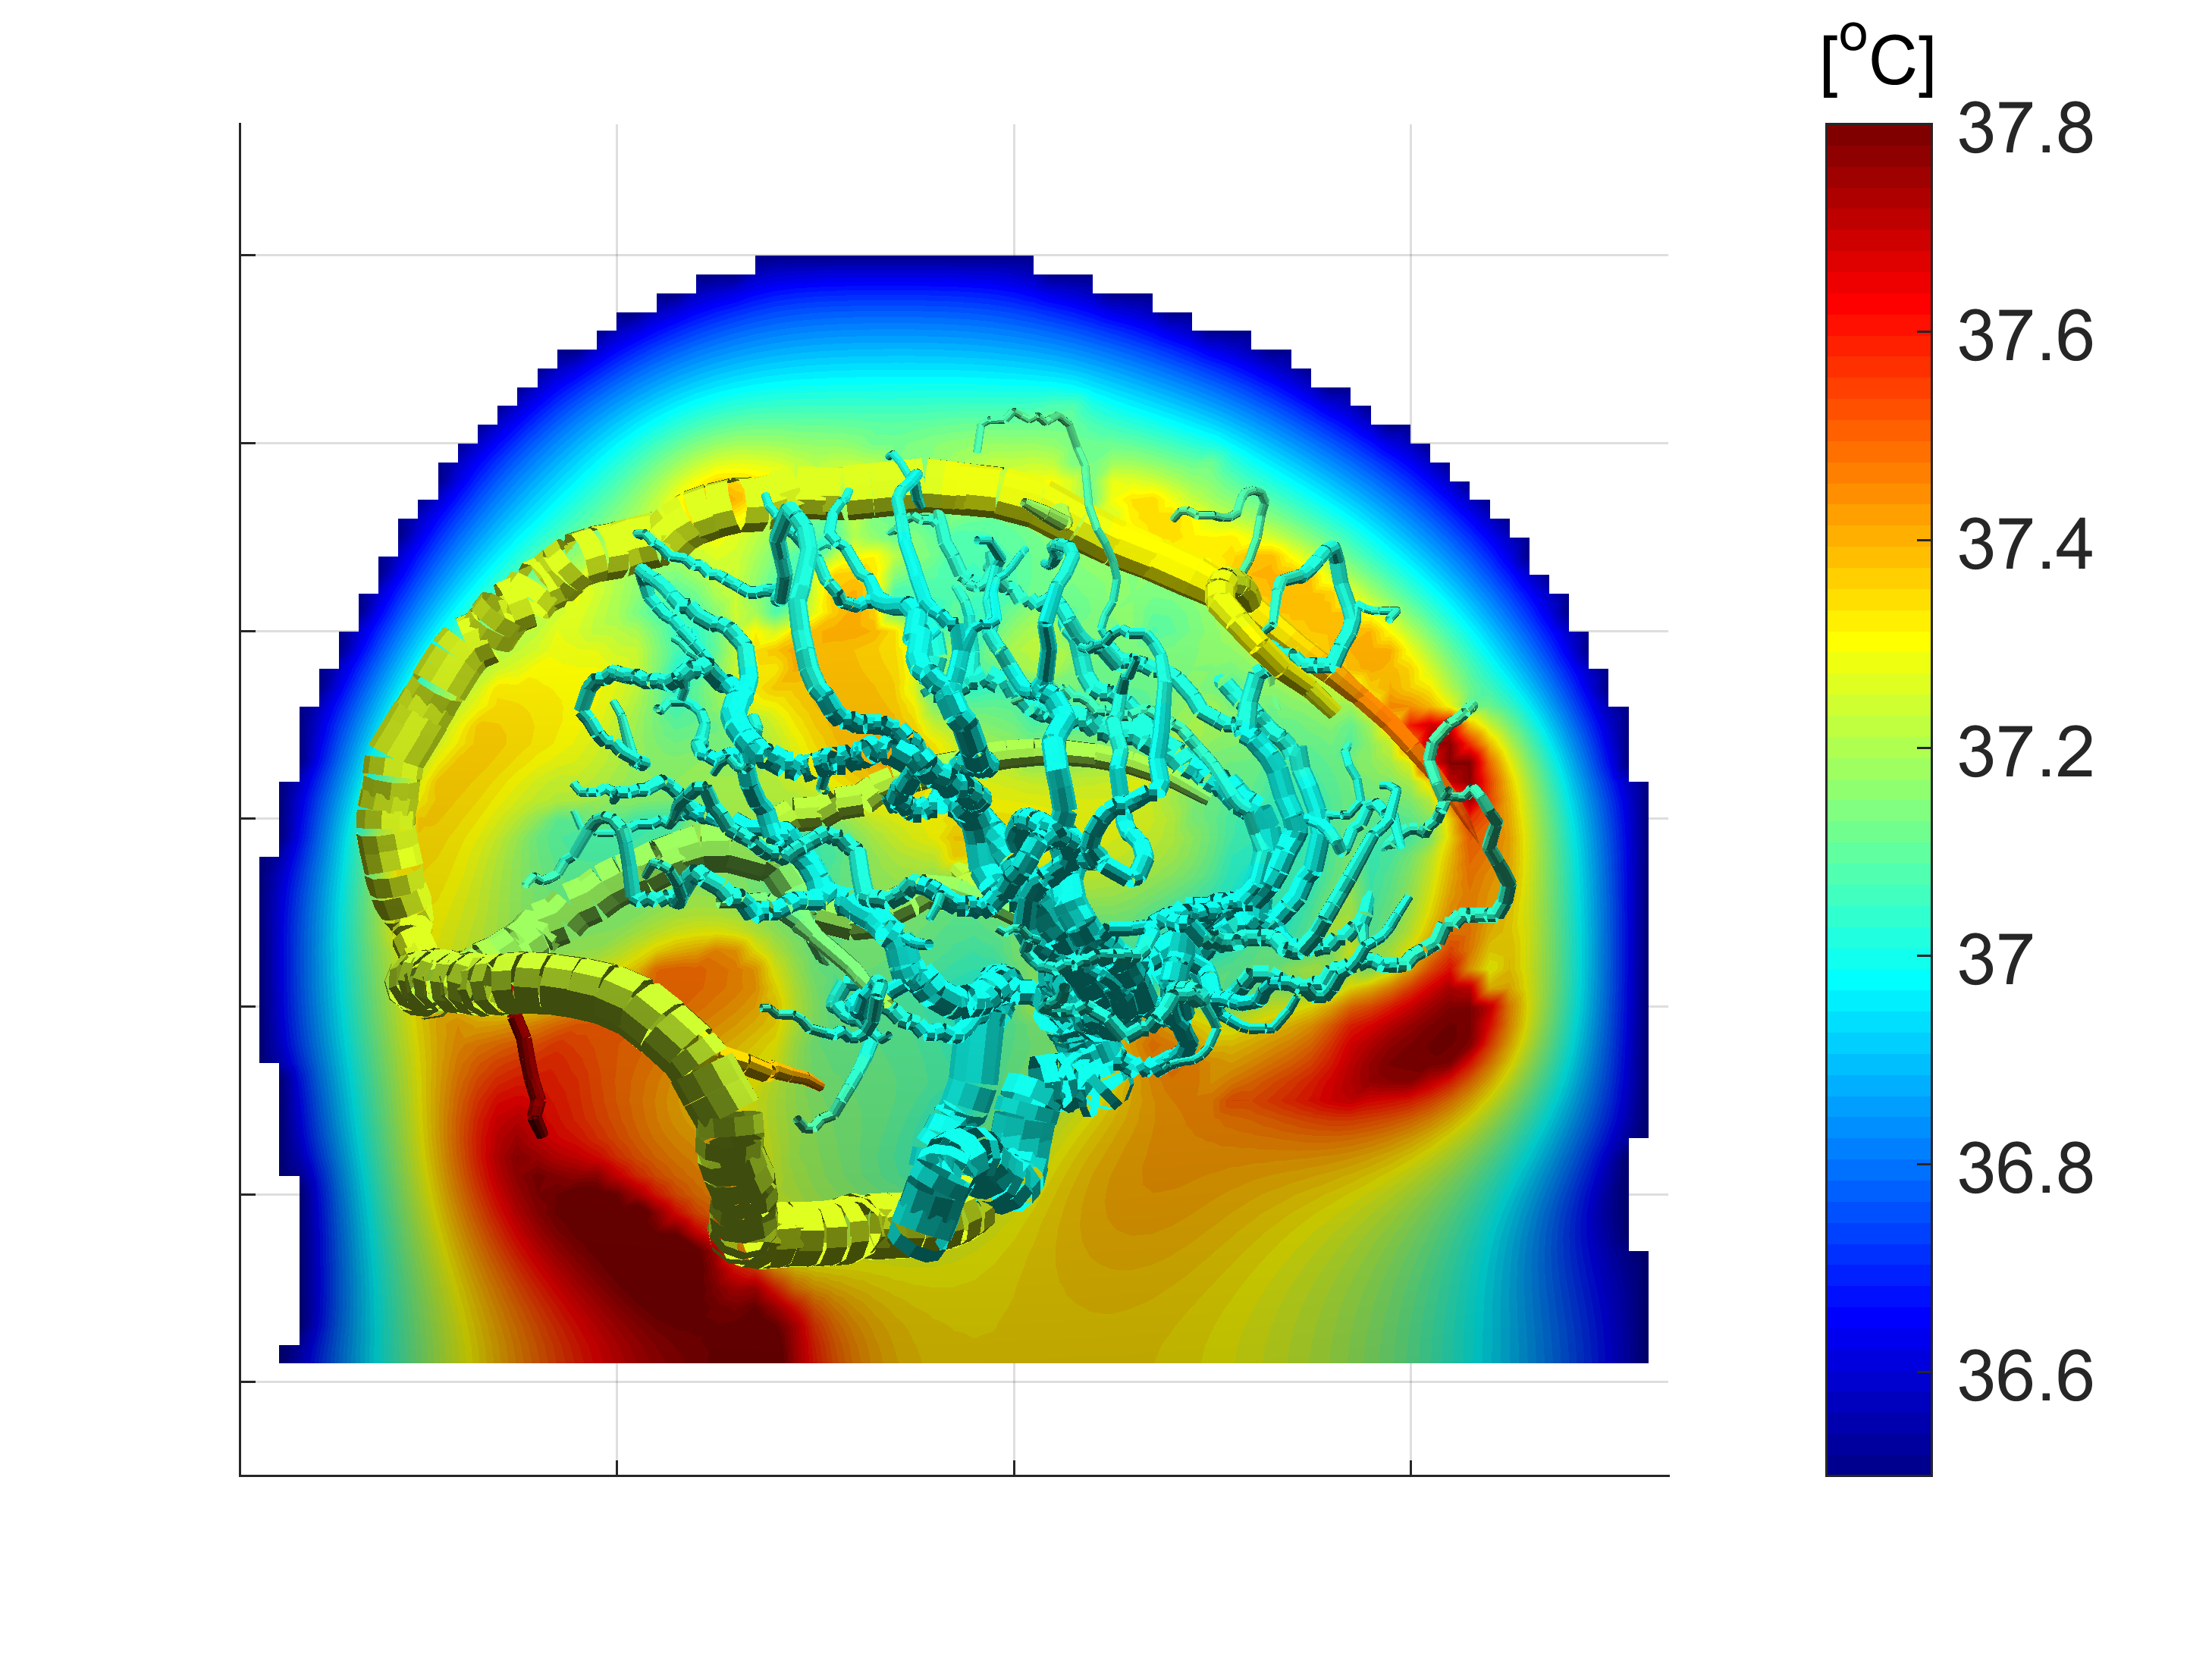
\includegraphics[width=0.49\textwidth]{Chapter3/Chapter3Result1}
	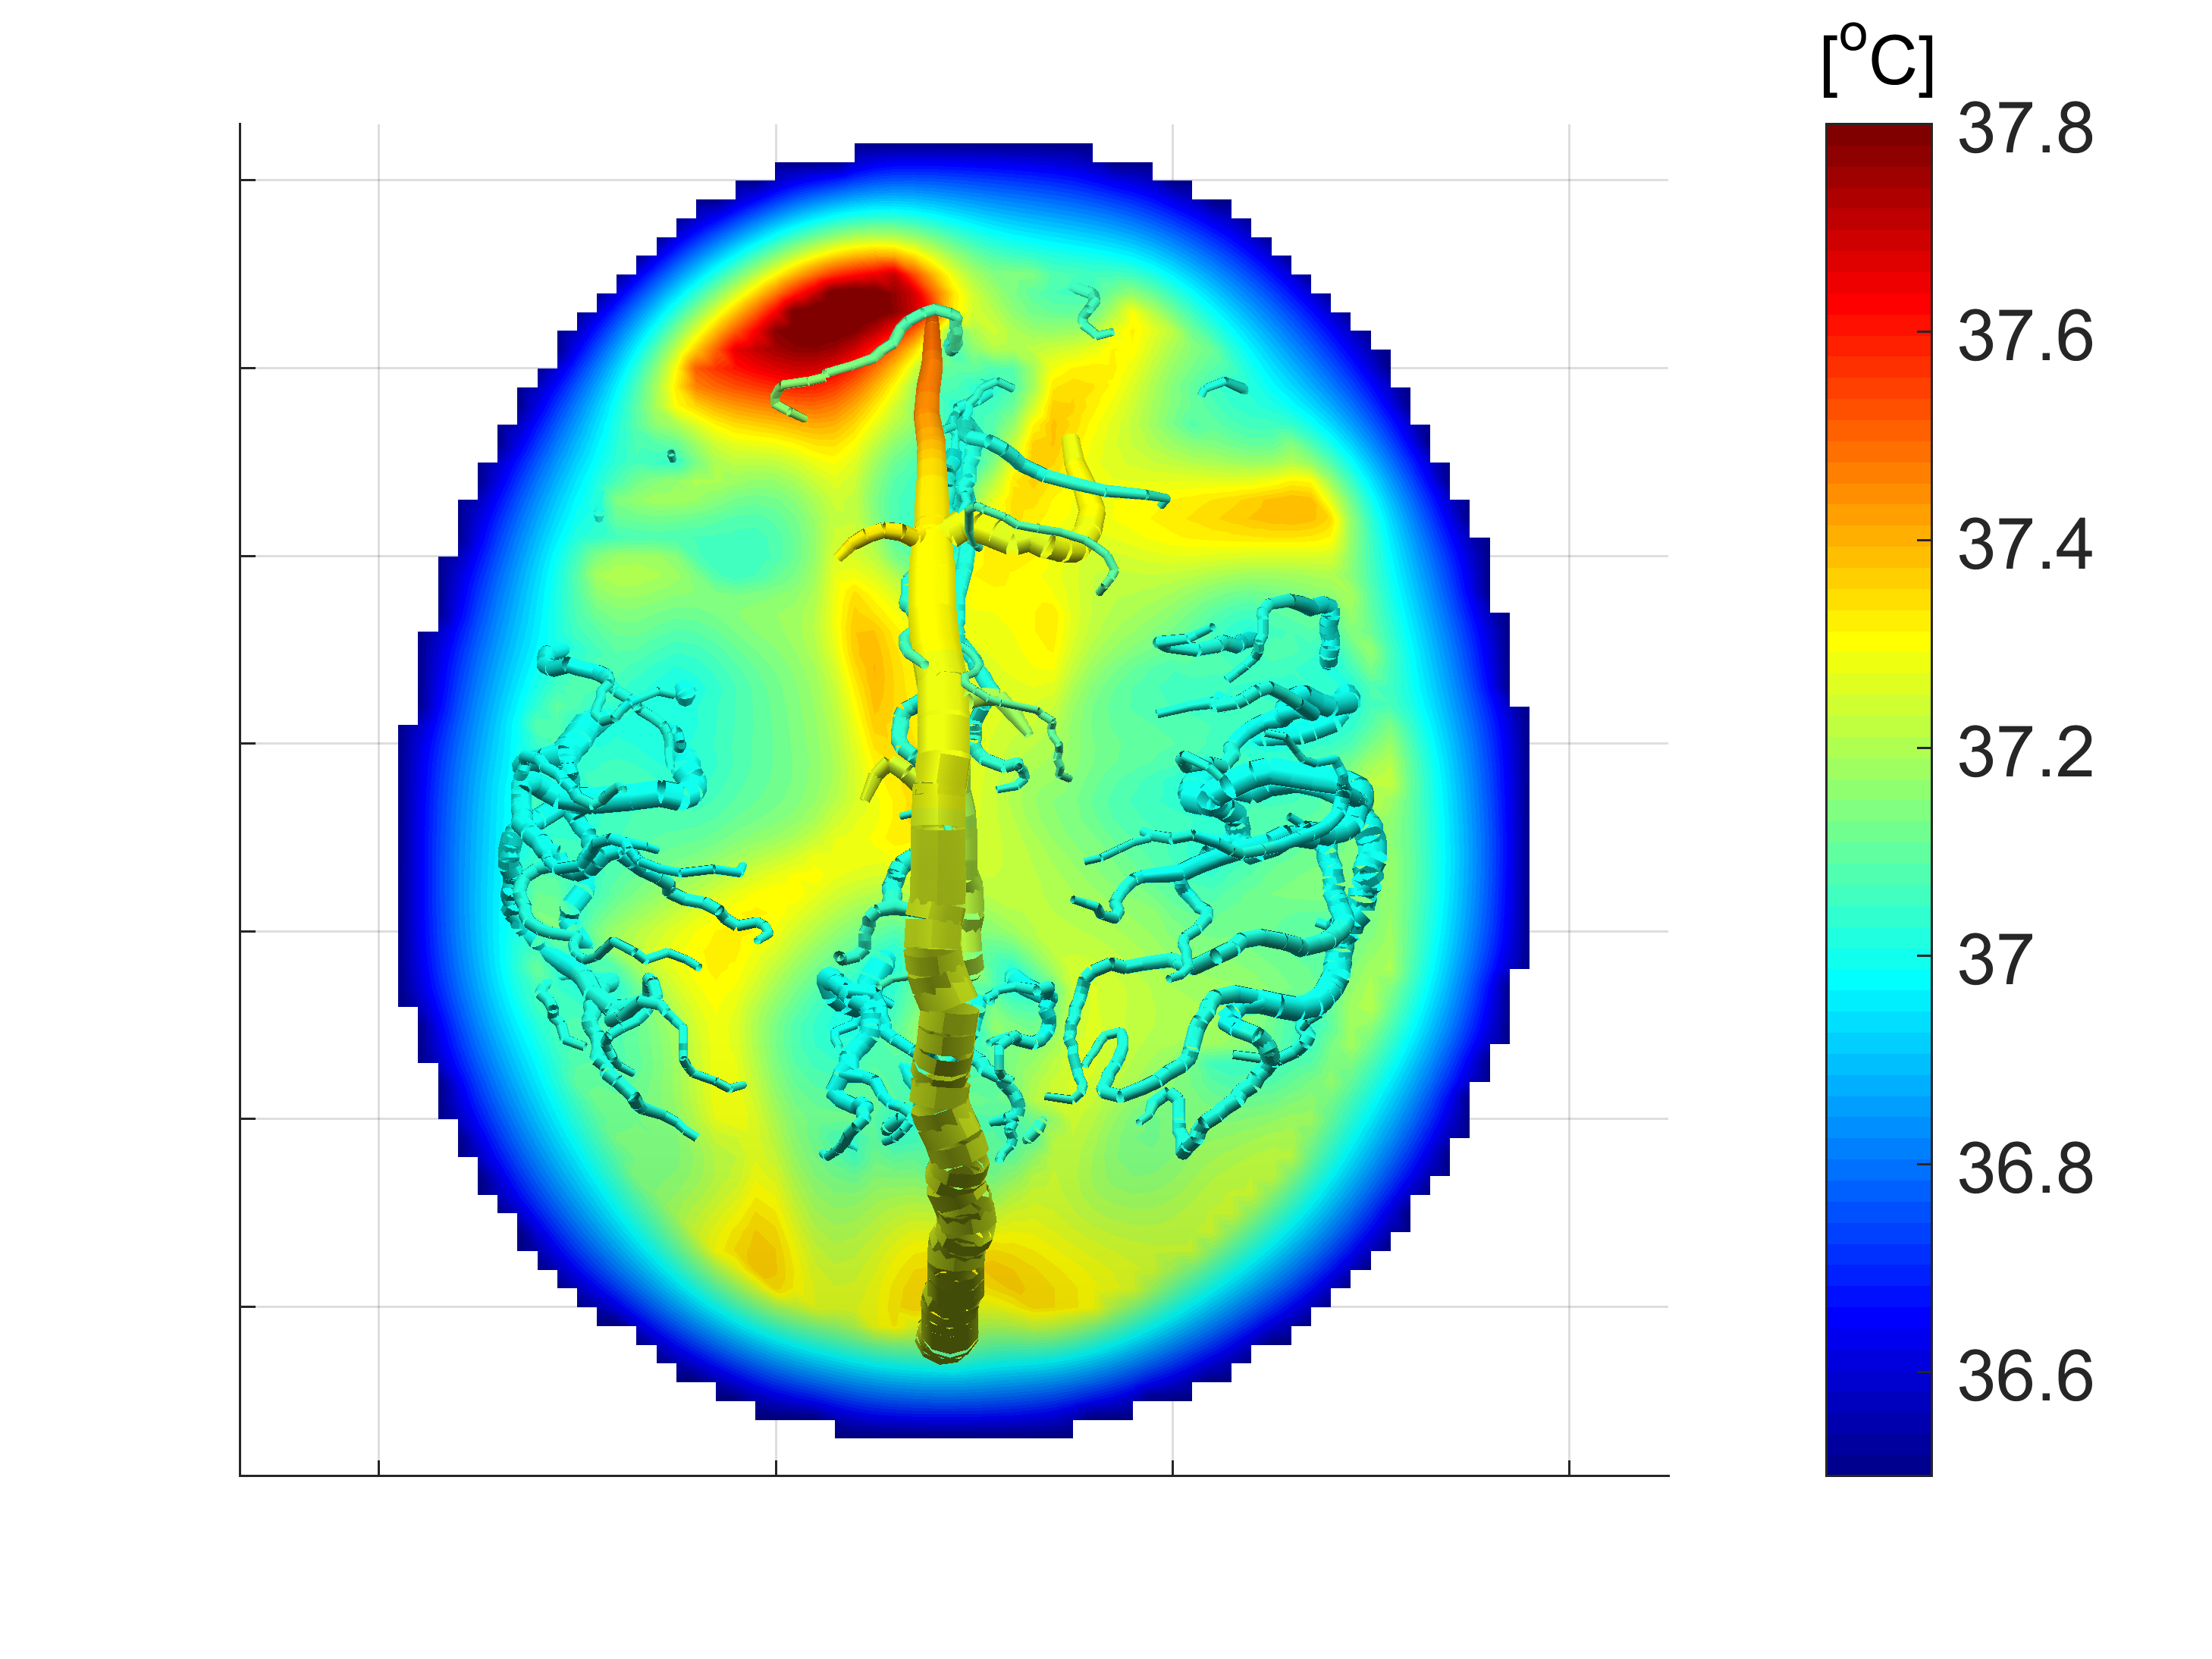
\includegraphics[width=0.49\textwidth]{Chapter3/Chapter3Result2}
	\caption[Profiles of tissue temperature  shown with vascular structure for a trial with no vessels generated at $T_{scalp}=36.5^{o}C$]{A sagittal (left) and axial (right) profile of tissue temperature shown with vascular structure for a trial with no vessels generated at $T_{scalp}=36.5^{o}C$.}
	\label{fig:Chapter3Results1}
\end{figure}

Figure~\ref{fig:Chapter3Results1} depicts a cross-sectional temperature profile derived using the base dense arterial and venous vessel trees with scalp temperature set at $36.5^{o}C$, similar to seen in the previous chapter. As before, regions at the anterior or the brain and within the cerebellum show higher temperatures than expected. The arteries and veins are relatively isothermal which suggests that most of the heat transfer is occurring within the capillary regions. Increasing the number of vessels should see the regions of higher temperature vanish as blood becomes more perfused. Additionally, more heat transfer between the vessels and the tissue is expected.

\begin{figure}[t]
	\centering
	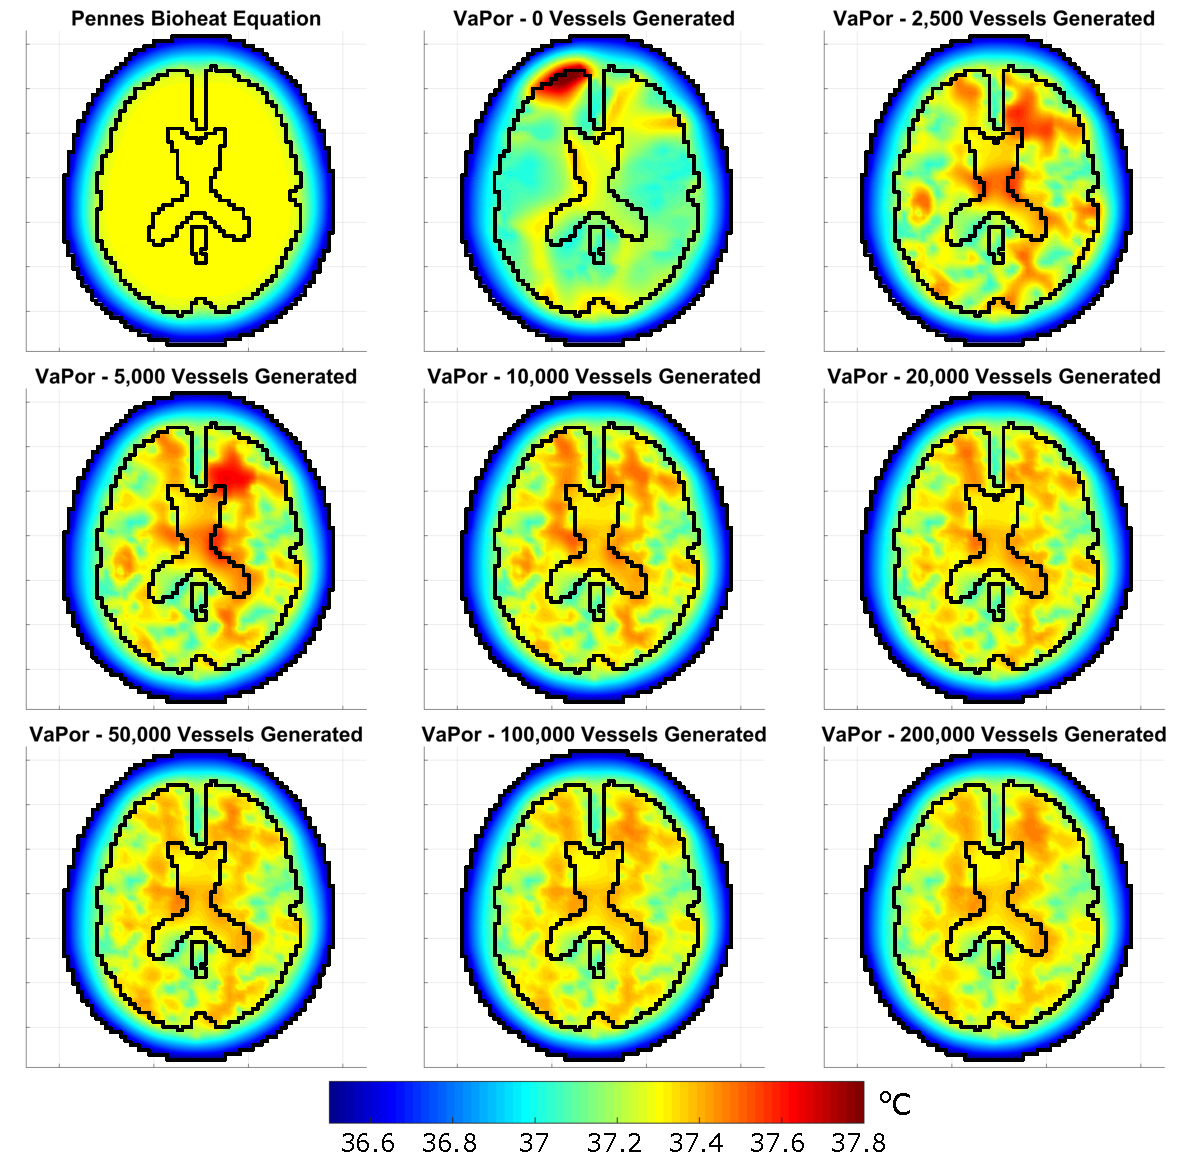
\includegraphics[width=0.9\textwidth]{Chapter3/TissueTemperatures}
	\caption[Tissue temperature profiles for scalp temperature of $36.5^{o}C$ using Pennes Bioheat Equation and the VaPor model at various levels of vessel generation]{Tissue temperature profiles for scalp temperature of $36.5^{o}C$. Top Left: Using Pennes Bioheat Equation only. Rest: Using the VaPor model. A single tree is used after various numbers of vessel generation iterations. Black lines depict head and brain domain boundaries.}
	\label{fig:TissueTemperatures}
\end{figure}

Figure~\ref{fig:TissueTemperatures} shows a temperature profile for the model under various iterations of vessel generation RRT-Algorithm. The average brain temperature for the Pennes Bioheat model is $37.29^{o}C$ and the average temperatures with vessels is $37.31^{o}C$ with negligible variation due to the number of vessels. With more vessels, there become fewer regions of high temperature due to the better distribution of blood. The maximum temperature within the brain with 0 generated vessels is $38.42^{o}C$, which is reduced to $37.52^{o}C$ with 200,000 vessels generated. Unfortunately, due to current memory limitations, 200,000 vessels is the limit for solving Equation~\ref{Eq:LinearSolver}. For a scalp temperature of $36.5^{o}C$, the difference between the profiles of 100,000 and 200,000 vessels is not substantial (root mean square of differences in temperature is $\pm0.01^{o}C$).  

\begin{figure}[t]
	\centering
	\includegraphics[width=\textwidth]{Chapter3/MeasuredPerfusions}
	\caption[Profiles of tissue perfusion using the VaPor model at various levels of vessel generation compared to the input perfusion used in Pennes Bioheat Equation]{Profiles of tissue perfusion. Top Left: The input perfusion used for Pennes Bioheat Equation and as a weighting function for generating vessels with the RRT-algorithm. Rest: Measured voxel perfusion values from the VaPor model. A single tree is used after various numbers of vessel generation iterations. Black lines depict head and brain domain boundaries. The different colourbars help to exhibit the large difference in magnitudes between results.}
	\label{fig:MeasuredPerfusion}
\end{figure}

Perfusion is the typical unit of measurement for blood flow within the brain \cite{sourbron2013classic}. It traditionally given in units of $ml/100g/min$ making it a measurement of volumetric flow per unit mass (or volume). This can be measured in the VaPor locally by summing up all the flowrates into each voxel and dividing by the mass of said voxel. The perfusion profile for Pennes Bioheat Equation shown in Figure~\ref{fig:MeasuredPerfusion} (top-left) are the local values for perfusion derived from the tissue weighted inputs from Table~\ref{tab:physicalparams2} and represent the desired output for measured perfusion. This depiction is similar to the profiles found in literature \cite{sourbron2009quantification}. The resultant values for perfusion seem to be orders of magnitude away from the input values. With higher numbers of vessels, the perfusion profiles appear to approach the input profile.

This discrepancy between measured values and values found in literature is not due to any mass imbalances but rather the method in which it is measured. By checking the flow in an out of every voxel it can be seen that mass flow is conserved in all locations. Although perfusion is the measurement of the overall blood flow through a specific volume, only flow considering to be perfusing the capillary bed should be measured. This is achieved clinically with the use of tracer distribution and is discussed further in the subsequent chapter. 

\begin{figure}[t]
	\centering
	\includegraphics[width=0.9\textwidth]{Chapter3/TissueDifferences}
	\caption[Tissue temperature difference profiles after reducing the scalp temperature from $36.5^{o}C$ to $10^{o}C$ using Pennes Bioheat Equation and the VaPor model at various levels of vessel generation]{Tissue temperature difference profiles after reducing the scalp temperature from $36.5^{o}C$ to $10^{o}C$. Top Left: Using Pennes Bioheat Equation only. Rest: Using the VaPor model. A single tree is used after various numbers of vessel generation iterations. Black lines depict head and brain domain boundaries. Only tissue within the brain is shown for clarity.}
	\label{fig:TissueDifferences}
\end{figure}

Figure~\ref{fig:TissueDifferences} shows the temperature differences after cooling the scalp from $36.5^{o}C$ to $10^{o}C$. The top-left image showing the results from the Pennes Bioheat Equation indicates that there is very little to no cooling in the core region of the brain. The average temperature drop for the whole brain using Pennes Bioheat Equation is $-0.44^{o}C$ and $-0.60^{o}C$ using the VaPor model with 200,000 vessels generated. Although this demonstrates a small increase overall, the main difference is that the cooling is spread out over more the brain as can be seen in Figure~\ref{fig:TissueDifferences} (bottom-right). If it is assumed that the voxels labelled white matter (those with weighting {$>$}$50\%$ in the tissue probability maps used) represent the core brain, then the core temperature change with using Pennes Bioheat Equation is $-0.12^{o}C$. However, in the VaPor model, with increasing number of vessels, a larger amount of the brain becomes cooled. The average core temperature change with 200,000 vessels generated is $-0.40^{o}C$. 

\begin{figure}[p]
	\centering
	\includegraphics[width=\textwidth]{Chapter3/StatisticsPlot}
	\caption[Effects of increasing the number of vessels generated in the VaPor model]{Effects of increasing the number of vessels generated in the VaPor model. The average values for 10 different trees are shown at 2,500, 5,000, 10,000, 20,000 50,000, 100,000, and 200,000 vessel generation iterations. Top Left: Average tissue temperatures. Top Right: Average decrease of tissue temperature after cooling. Middle Left: Average decrease of tissue temperature after cooling in grey matter. Middle Right: Average decrease of tissue temperature after cooling in white matter. Bottom Left: The combined volume of vessel trees as a percentage of brain volume. Bottom Right: The average measured perfusion in voxels. The error bars depict standard deviation. The error bars in Top Left and Bottom Right are too small to visualise}
	\label{fig:ResultsGraphs}
\end{figure}

The generation of vessels has a degree of randomness to it so the results have some variability between trials. Figure~\ref{fig:ResultsGraphs} shows the averages and variation for certain parameters across the growth of 10 separate vessel trees. It shows that increased cooling with increased number of vessels is consistent across all trials. All results appear to be approaching a plateau, however, due to the memory limitations, analysis of larger vessel trees is not possible for temperature results. 

\section[Analysis of Model]{{\Large A}nalysis of {\Large M}odel} 
\fancyhead[RO]{\makebox[1cm][r]{\fontfamily{ppl}\small\thesection{ -- }\scriptsize\MakeUppercase{{\small A}nalysis of {\small M}odel}}\enskip$\mid$\makebox[1cm][l]{\enskip\fontfamily{ppl}\thepage}}

There are too many variables and physical parameters within the VaPor model to do a full sensitivity analysis on each. Additionally, some parameters might not be sensitive under certain conditions but highly sensitive in others. Many of the physical parameters such as thermal conductivity and perfusion have been varied in previous works \cite{xuan1997bioheat}\cite{zhu2001theoretical}\cite{van2000numerical} and the VaPor model agrees with the trends shown there.

Adjusting the porosity, capillary diameter, or capillary tortuosity by a factor of $0.5$ or $5$ resulted in negligible changes to temperatures. These factors only affected the magnitudes of pressure drops within the 3D model but did not have much effect on the direction of flow. This shows that the geometry of vessels is much more important for flow distribution than the physical parameters of the capillary domain.

Domains 1 \& 4 are super-imposed inside domains 2 \& 3 but there is no volume fraction associated with them. The volume taken up the vessels as a percentage of total brain volume is shown in Figure~\ref{fig:ResultsGraphs} (bottom-left). It was assumed that the volume of these vessels would be small enough that the effect of their volumes would be negligible. The volume fraction of vessels is approaching the input values used for tissue porosity so it is possible that this assumption is incorrect and that the the values for porosity should be adjusted to take into account the volume of blood in domains 1 \& 4. However, the porosity was already assessed for sensitivity and found to have little effect on the temperature results. A single tree generated with 500,000 vessels showed a volume fraction of 4.2\% which agrees with the speculation that the graphs are plateauing.

\subsection{Mesh Dependency} 

\begin{figure}[h]
	\centering
	\includegraphics[width=0.49\textwidth]{Chapter3/MeshDependency_Corr}
	\includegraphics[width=0.49\textwidth]{Chapter3/MeshDependency2}
	\caption[Variations of tempeature and brain volume with decreasing voxel size]{Left: Variation of average tissue temperatures with voxel size. Diamonds and solid line represent a trial with no vessels generated. Circles and dashed lines represent a trial with 50,000 vessels generated. The colours red and blue denote scalp temperature of $36.5^{o}C$ and $10^{o}C$ respectively. Right: Variation of total brain volume with voxel size. The dashed line depicts the predicted volume at higher resolutions as the data is given at a resolution of $1.5mm$.}
	\label{fig:MeshDependency}
\end{figure}

As this model has been developed from the ground upwards, certain parameters need to be checked to determine the model functions as intended. Direct validation of results is not possible due to lack of availability of data for brain temperatures. Whilst certain methods allow a prediction of brain temperatures through scans \cite{marshall2006measurement}, the accuracy of these methods is not agreed upon \cite{thrippleton2014reliability}. 

Simple mass and energy balance checks throughout the model show that these parameters are conserved. The only variation appears from machine rounding errors of the order $10^{\smallminus14}$, far lower than any flowrate or temperature value, so they can be ignored. 

A mesh dependency test was performed to ensure that the 3D grid used was refined enough that the results were not affected. The grid was divided up in cubic voxels of $2.25mm$, $3.0mm$, $4.5mm$, and $9.0mm$ and run with both the base vessel trees and with 50,000 vessels generated. Figure~\ref{fig:MeshDependency} (left) shows the average temperatures for scalp temperatures at both $36.5^{o}C$ and $10^{o}C$. At coarser grid sizes, the effect of cooling is much more pronounced, especially with increased numbers of vessels. However, the difference of temperatures produced between a grid size of $3mm$ and $2.25mm$ is small (root mean squared difference of temperatures {$<$}$1\%$ of average temperature). Therefore, a grid size of $3mm$ was considered sufficient for the purposes of modelling. All simulations were performed at this grid size unless specified otherwise.

Due to the coarsening of the voxel size, the actual volume of brain changed within the simulation as shown by Figure~\ref{fig:MeshDependency} (right). This is due to the imposed discretisation between grey and white matter and other tissue types to represent the brain. As the grid is coarsened, the voxels on the fringe of the brain become more convoluted by other tissue types so fewer voxels are part of the brain domain. This has an effect on the total blood flowrate which is directly proportional to brain volume within the model. The lower blood flowrate could also explain the increased sensitivity to cooling at larger voxel sizes.

The grid sizes of the vessels were also explored by sub-dividing the line segments into smaller fragments. However, when increasing the size of the vessel trees through the RRT-Algorithm, this sub-division is performed regularly as newly generated line segments are joined onto existing ones with a sub-division occurring at the intersection. Taking a vessel tree with 50,000 generated vessels and dividing all line segments into four equal parts reduced the magnitude of core cooling by $0.06^{o}C$. However, when the sub-divisions occur from increasing the number of vessels through the RRT-Algorithm, the magnitude of core cooling is increased.  

\subsection{Comparison with Ansys CFX 16.0 Flow Solver}

In order to validate the solutions to the energy balance and the mass and momentum balance produced by the VaPor model, a comparison was made against results generated within Ansys CFX for an equivalent mesh structure. The 1D vessels used in the VaPor model cannot be computed in Ansys CFX so only the basic flow and energy equations are used in this validation.

To avoid complications from geometries, a basic cubic structure was used with similar conditions used in the brain model. There is only a single inlet and outlet set at opposite corners of the cube, modelled as source points in Ansys CFX and as a single artery and vein in the VaPor model. All other variables are the same within both models.

For simplicity, the structure was chosen to be a, initially with 20 voxels on each length, and later refined to 50 voxels on each length. Heat transfer was performed on 5 of the six faces, the adiabatic face being proximal to the inlet. The cube edges had a length of 11.4cm so that the overall volume of the cube was 1,481.5$cm^{3}$. The tissue was considered isotropic so no segmentation between grey and white matter was included. Porosity was fixed at $\epsilon_{b}=0.05$, metabolism rate was fixed at 10,437$W/m^{3}$, and perfusion was fixed at $50ml/100g/min$. 

\begin{figure}[h]
	\centering
	\includegraphics[width=\textwidth]{Chapter3/AnsysComparison}
	\caption[Comparison of VaPor model with Ansys CFX 16.0 in a simple cubic geometry]{Comparison of VaPor model with Ansys CFX 16.0 in a simple cubic geometry. Left: Schematic of the simulation. The red and blue circles represent the inlet and outlet respectively. The bottom shaded surface depicts the adiabatic face. Right: Profiles of superficial velocity (top row) and tissue temperature (bottom row) for the VaPor (left) and Ansys CFX (right) models. The plane in question is half way up the cube shown by the dashed line in the schematic.}
	\label{fig:AnsysComparison}
\end{figure}

Ansys CFX stores values at the nodal points of the mesh whereas the VaPor model uses the volume centred values. Therefore, the Ansys CFX results were linearly interpolated to the volume centred values for comparison. The results from the VaPor model and the Ansys CFX equivalent show very good agreement.  Average deviation of velocities is $1.09\%$. Average deviation of temperatures for the normothermia and cooling conditions are $0.055\%$ and $0.46\%$ respectively. When the grid was refined to 50 voxels on each length of the cube, the results maintain their accuracy. Average deviation of velocities is $0.72\%$. Average deviation of temperatures for the normothermia and cooling conditions are $0.037\%$ and $0.29\%$ respectively. This demonstrates that the flow and temperature models used within VaPor function as expected compared to commercial software.

\subsection{Arterial Inlet Temperatures} 

\begin{figure}[h]
	\centering
	\includegraphics[width=0.49\textwidth]{Chapter3/InletTemperatures}
	\caption[Variation of average tissue temperature with arterial inlet temperature for a model with 50,000 generated vessels]{Variation of average tissue temperature with arterial inlet temperature for a model with 50,000 generated vessels. The dashed line depicts predicted temperature rise from total metabolism and blood thermal capacity given by $T = T_{a}+\frac{\overline{Q}_{gen}}{\rho_{b}c_{b}}$.}
	\label{fig:InletTemperatures}
\end{figure}

\begin{figure}[h]
	\centering
	\includegraphics[width=\textwidth]{Chapter3/SpecificInletTemperatures}
	\caption[The effects of reducing a single arterial inlet temperature to $35^{o}C$ for a model with 200,000 generated vessels]{The effects of reducing a single arterial inlet temperature to $35^{o}C$ for a model with 200,000 generated vessels. Left: Cooling the rear basilar artery. Middle: Cooling the left internal carotid artery. Right: Cooling the right internal carotid artery. This method also helps to highlight which regions of the brain are fed by each inlet in the model.}
	\label{fig:SpecificInletTemperatures}
\end{figure}

It has been demonstrated before that cerebral temperature is heavily influenced by core body temperature and by extension inlet arterial temperature \cite{konstas2007theoretical}\cite{van2000numerical}. Figure~\ref{fig:InletTemperatures} shows that the VaPor model agrees with this in that there is an almost perfectly linear relationship between cerebral and core body temperatures. The dotted line shows the predicted rise in temperature due to the the energy production from metabolism and thermal capacity of blood (given by: $T = T_{a}+\frac{\overline{Q}_{gen}}{\rho_{b}c_{b}}$). There is almost perfect agreement save for slight deviation due to the external influence of scalp temperature. This demonstrates that the core body temperature has a much larger influence on brain temperature than scalp temperature. Although not shown, varying the metabolism rate or the thermal capacity shifts the resultant temperature vertically at the same rate as the predicted curve. 

Figure~\ref{fig:SpecificInletTemperatures} shows that cooling a single arterial inlet to $35^{o}C$ cools a specific region of the brain. This also demonstrates the flow network functions as expected. Flow entering the left internal carotid artery feeds the left hand side of the brain and vice versa. The basilar artery predominantly feeds the posterior cerebral artery but has a smaller magnitude of flow than the other inlets so the effect is much less pronounced. 

\subsection{Vascular Generation and Modelling Methods}

The results depicted here are based on the assumption that the traversal of blood between vessels and capillaries (i.e.\ domains 1 \& 4 to and from domain 3) happens within all vessel segments. The idea being that the transfer would occur in small arterioles and venules attached to these branches that are not necessarily modelled. In reality, the transition between vessels and capillaries occurs only where the smallest arterioles and venules divide. Therefore, a more physiological representation for this in the VaPor model would be to confine any transfer of blood between these domains to the branch terminations of the vessel trees. 

Additionally, the simpler form of the RRT-Algorithms was used throughout the trials. An alternative form of the algorithm was presented (see Section~\ref{Sec:3AcquiringBloodVesselData}) but not used due to lower distribution  produced at fewer generation iterations and a longer computational time. Neither method is inherently based on physiology, save for the weighting by local perfusion, however, the structure of the trees differ, as shown in Figure~\ref{fig:RRTComparison}.

To demonstrate that the results shown are not an inherent factor of these conditions, a sample of results are shown in Table~\ref{Tab:VesselsVerification} for 200,000 generated vessels. Four trials were considered with a different combination each of the two methods of the RRT-Algorithm and either having the vessel/voxel transitions confined only to branch terminations or occurring at all vessel segments. The change in values are not significant and easily fall within the ranges shown in Figure~\ref{fig:ResultsGraphs}. The profiles shown in  Figure~\ref{fig:VascularGenerationType} for perfusion and temperature difference after cooling are from a simulation that used both the alternative RRT-Algorithm and vessel/voxel transitions occurring only at branch terminations. These are qualitatively very similar to the corresponding profiles in Figure~\ref{fig:MeasuredPerfusion} (bottom right) and Figure~\ref{fig:TissueDifferences} (bottom right) respectively.

\begin{table}
	\centering
	\fontsize{8pt}{9pt}\selectfont
	\begin{tabular}{m{4.5cm}C{1.3cm}C{1.3cm}C{1.3cm}C{1.3cm}}
		\toprule
		\textbf{Measured Parameter} & \textbf{RRT-1, BT: } \text{\sffamily \textbf{X}} & \textbf{RRT-1, BT: } \cmark & \textbf{RRT-2, BT: } \text{\sffamily \textbf{X}} & \textbf{RRT-2, BT: } \cmark\\
		\hline
		Average Perfusion [$ml/100g/min$] & 81.7 & 85.1 & 82.5 & 88.7 \\
		Average Temperature Drop After Cooling [$^{o}C$] & 0.60 & 0.59 & 0.60 & 0.60 \\
		Average Temperature Drop After Cooling, White Matter Only [$^{o}C$] & 0.40 & 0.41 & 0.40 & 0.41 \\ \bottomrule
	\end{tabular}
	\caption[Comparison of results for different types of vascular generation and modelling options for 200,000 vessels generated]{Comparison of results for different types of vascular generation and modelling options for 200,000 vessels generated. RRT-1 and RRT-2 denote the original and alternative vessel generation algorithms respectively. The tick and cross next to BT denote whether vessel/voxel mass flow transitions are limited to branch terminations only or not respectively.}
	\label{Tab:VesselsVerification}
\end{table}

\begin{figure}[h]
	\centering
	\begin{subfigure}[b]{0.49\textwidth}
		\includegraphics[width=\textwidth]{Chapter5/Chapter5_1b}
	\end{subfigure}
	\begin{subfigure}[b]{0.49\textwidth}
		\includegraphics[width=\textwidth]{Chapter5/Chapter5_1a}
	\end{subfigure}
	\caption[A profile of tissue perfusion and a profile of tissue temperature difference after cooling for a trial using both the alternative vessel generation algorithm and with blood transfer occurring only at branch terminations with 200,000 generated vessels]{A profile of tissue perfusion (left) and a profile of tissue temperature difference after cooling (right) for a trial using both the alternative vessel generation algorithm and with blood transfer occurring only at branch terminations with 200,000 generated vessels. Black lines depict head and brain domain boundaries.}
	\label{fig:VascularGenerationType}
\end{figure}

\subsection{Incorporating Thermal Inlet Effects}

The Nusselt number used is based on the average wall heat transfer for a flow that is fully thermally developed. For laminar flow, this means that the cross-sectional temperature profile is parabolic, with the temperature at the walls being lower than the average temperature, reducing the driving force necessary for the thermal exchange. However, due to the tortuous nature of blood vessels, the flows within the vessels are subject to mixing, which disrupts the cross-sectional temperature profile leading to slightly higher heat exchange at the walls. This is one of the reasons that a single temperature is used for the vessels as the blood is assumed to be thermally well mixed \cite{kotte1996description}. 

The effect of the thermally developing region on overall heat transfer can be determined using a correlation between the Nusselt number and the Graetz number \cite{peattie2012transport}:

\begin{equation}
\Nuss = 4 + 0.155e^{1.58\log_{10}(Gz)}
\label{Eq:GraetzNumberNusselt}
\end{equation} 

With the Graetz number, \Graetz, being given in terms of vessel mass flowrate, $\dot{F}$, and average segment diameter and cross-sectional area as:

\begin{equation}
\Graetz = \frac{c_{b}\dot{F}(D_{v}+D_{adj})^{2}}{4A_{Xsec}K_{b}L_{v}}
\label{Eq:GraetzNumber}
\end{equation} 

With $A_{Xsec}$ being defined from Equation~\ref{Eq:CrossSectionArea}. The flowrates for each segment used here are the values prior to mass exchange with the tissue. Equation~\ref{Eq:GraetzNumberNusselt} is only valid for $\Graetz{<}1000$ so the results were capped at $\Nuss=20$ to prevent over-exaggeration of the heat transfer.

\begin{figure}[h]
	\centering
	\includegraphics[width=0.7\textwidth]{Chapter3/Chapter3_GraetzHistogram}
	\caption[A histogram of Nusselt numbers for vessels after applying the thermal inlet effect]{A histogram of Nusselt numbers for vessels after applying the thermal inlet effect with Equation~\ref{Eq:GraetzNumberNusselt}. There are a small number of vessels that are capped with $\Nuss=20$ but the vast majority lie within the range $4{<}\Nuss{<}8$.}
	\label{fig:GraetzHistogram}
\end{figure}  

Figure~\ref{fig:GraetzHistogram} shows the effect Equation~\ref{Eq:GraetzNumberNusselt} had on the Nusselt number for a simulation with 200,000 vessels generated. The majority of vessels are not affected by this, showing an increase of {\Nuss} by less than 0.08. A small number of vessels reach the capped limit of $\Nuss=20$ due to possessing larger flowrates combined with shorter segment lengths. These therefore have the inter-domain heat exchange increased by five-fold which can promote thermal circulation through the brain. 

When introduced, the average temperature decrease after cooling for the whole brain and core white matter increased by 5.1\% and 11.1\% respectively. This demonstrates that the thermal inlet effect increases heat transfer with the vessels and promotes core cooling. However, using Equation~\ref{Eq:GraetzNumberNusselt} for all vessels assumes that the blood is fully mixed at the entrance to every segment in the vessel tree. This is unrealistic as, although tortuous, the flowrates within the capillaries are too small to achieve this reliably. Therefore, this represents a best case scenario and the actual impact of the inlet effect is almost certainly lower than this. As the actual impact is unknown, the inlet effect is not used in other models and the heat transfer between vessels and tissue is kept constant with $\Nuss=4$.

\section[Discussion]{{\Large D}iscussion}
\fancyhead[RO]{\makebox[1cm][r]{\fontfamily{ppl}\small\thesection{ -- }\scriptsize\MakeUppercase{{\small D}iscussion}}\enskip$\mid$\makebox[1cm][l]{\enskip\fontfamily{ppl}\thepage}}
\label{Sec:3Discussion}

In this chapter, the theoretical framework for the VaPor model was presented. Additionally, a selection of results and analysis of the model was shown.

The VaPor model allows the simulation of both blood and temperature flow using mass and temperature interaction of 1D and 3D domains. This gives the model high flexibility for adjustment and allows the vessels to be expanded upon with ease.

The analysis of results have shown that the base equations agree with the Ansys CFX package used in the previous chapter. Additionally, temperatures produced by the model fall within the expected range of temperatures. Validation of the model is not possible as there is little data to compare results against (agreement with available data from rat brains \cite{zhu2006body} is shown later on in Section~\ref{Sec:5RatBrains}). Additionally, due to the natural variation of biological structures person to person, an exact solution cannot be found. Instead, this model serves to look at the broad effects of including full convective blood flow for simulating biological temperatures.

The sole addition of the base vessel trees and porous media did not make a large difference on temperature drops after cooling, even though it does add directionality to the model. The core regions of the brain still remained unaffected by the change of scalp temperature. Only with large number of vessels added (in the order of $10^{5}$) did the VaPor model display larger degrees of core cooling than Pennes Bioheat Equation. This contradicts the theory put forward by Chato \cite{chato1980heat} that vessels below $0.2mm$ become thermally insignificant. The vessels produced by the model have generally have branches of {$<$}$0.2mm$ after 20,000 iterations. If the vessels below this diameter were thermally insignificant, then the temperature profiles produced would be the same regardless of the number of vessels generated after this point. However, Figure~\ref{fig:ResultsGraphs} shows that there is a definitive effect from these smaller vessels. 

Although the vessels of this size rapidly reach thermal equilibrium with the surroundings, as shown by Chato \cite{chato1980heat}, the directional flow included with them aids in the heat transfer between voxels. Without vessels, the convective transfer of heat between voxels is achieved with Equation~\ref{Eq:3DConvection} which only allows for transfer unidirectionally downstream. If, instead, the blood is transported through a highly tortuous network of vessels, the convective transfer between voxels would be back and forth as the vessels cross the voxel boundaries multiple times. This effectively increases the heat transfer between voxels. It is similar in principle to the Weinbaum and Jiji model \cite{weinbaum1985new} in which the counter-current heat exchange from nearby arteries and veins can be replaced with an increased effective conductive heat transfer coefficient. 

As $\beta_{2,3} = \infty$ is used in the model, there was concern that a similar effect to the 1D Counter-Current model shown in Section~\ref{Sec:21DHemisphere} whereby un-physical results are obtained due to the convective flows cancelling out. Although the results lie within expected values, a similar effect could explain the increased core cooling as convective flow across voxel boundaries are cancelled out. A Counter-Current model similar to that introduced in Section~\ref{Sec:21DHemisphereTheory} was applied to the VaPor model but it is presented in Chapter~\ref{Sec:5Chapter5}.

Increasing the number of vessels led to values for measured perfusion approaching input values and profiles found in literature. However, this does not necessarily mean the model became more accurate with increased number of vessels, only that the method for measuring perfusion became more in line with the method performed clinically. As \text{in-vivo} values of perfusion are obtained through injecting a tracer through the circulatory system, the generation of perfusion values from the VaPor model is not as straight forward as presented here. This is discussed in more detail in the following chapter.  

The generation of vessels was performed using a relatively basic space filling RRT-Algorithm for the purposes of simplicity. There exist other methods that produce biologically representative models that can be weighted by factors such as desired perfusion or oxygen requirement in tissue \cite{schreiner1993computer}\cite{schneider2012tissue}. These tend to adhere more to the established rules that govern blood vessel growth than the algorithm used in the current model. Including a more robust vessel generation algorithm would only benefit the VaPor model and, if diameters of vessels could be produced via a growth algorithm, there would not be any more need to iterate using the relationship given in Table~\ref{tab:DtoFlow}. Although having different appearances, the two methods for generating vessels shown in Figure~\ref{fig:RRTComparison} give near identical results once enough vessels had been generated to sufficiently fill the domain. This is due to both methods increasing the inter-voxel heat exchange as discussed above and it is expected that this will occur with other vessel generation algorithms. Therefore, the simplicity of the method for vessel generation used in the VaPor model is not expected to be a major drawback in the overall model.

Another assumption made with the vessels is that blood is transferred from domains 1 \& 4 at each line segment. Although in reality, there is no transfer of blood from larger arteries or veins directly to capillaries but rather first through a hierarchy of small arterioles or venules. This would mean transfer within domains should only occur at branch terminations. This was not implemented in order to allow trials with low numbers of vessels to have more distribution. However, with increasing number of vessels, the ratio of branch terminations to non-branch termination segments steadily increases. Therefore, if inter-domain flow is limited to only branch terminations with 200,000 vessels generated, there is little difference to the outcome. 

\subsection{Comparison to Previous Bioheat Models}

Previous bioheat models that rely solely on the Pennes Bioheat Equation show that core brain cooling should not be possible with scalp cooling alone \cite{nelson1998brain}\cite{sukstanskii2004analytical}\cite{zhu2001theoretical}. In the previous chapter, the addition of directional flow increased the effect of scalp cooling on the brain temperatures, especially flow directed inwards from the scalp. The VaPor model allows for proper 3-Dimensional flows to be investigated. In doing so a larger degree of core brain temperature reduction is observed. The absolute change is small, less than $1^{o}C$ for all models, however, changes as small as $0.3^{o}C$ could still be clinically relevant \cite{mariak2002intracranial}. 

The DiVa model is similar in structure to the VaPor model in that it includes 1-Dimensional vessels, but only to the thermally significant diameter given by Chato \cite{kotte1999modelling}. The results showed good agreement with Pennes Bioheat Model in that scalp cooling does not affect core brain temperatures \cite{van2000numerical}. Similarly, the VaPor model with relatively low levels of vessel generation displayed a lack of core brain temperature reduction. However, with larger numbers of vessels, there was higher magnitude of white matter temperature drop as shown in Figure~\ref{fig:ResultsGraphs} (middle-right). At the highest levels of vessel generation, the inter-voxel mass transfer tends to zero as blood would only transition from domain 1 to domain 4 through the same voxel. This would then make the VaPor and DiVa models very similar in execution and similar results would be expected. Unfortunately, a working DiVa was not available for direct comparison.

It is worth noting at this point that the reason the increased temperature drop with large number of vessels was discovered in this model and not with the previous DiVa model is due to the inaccurate measurements for perfusion generated by the VaPor model. By having the porous media transport blood in between arteries and veins, the distributing flows caused over-estimation of local perfusion value. In contrast, as blood is delivered directly from arteriole to voxels not necessarily immediately adjacent, this issue is circumvented and the expected values for perfusion can be achieved with relatively low numbers of vessels. Although the use of porous media does not have much of an effect on heat transfer after 200,000 vessel generation iterations, its implementation led to the cooling effect of numerous vessels to be discovered. 

Neimark~\textit{et al.\ }\cite{neimark2007integration} modelled intracarotid cooling using Pennes Bioheat Equation, whereby predicted flow values from a circle of Willis model distributed flows in a compartmentalised brain. A similar effect is seen in Figure~\ref{fig:SpecificInletTemperatures} where compartmental zones can be observed when cooling individual arterial inlets. A further trial was performed simulating intracarotid cooling combined with a cooling cap \cite{neimark2008brain}. Although, with the cooling cap alone, similar results were seen as before, after intracarotid cooling, the cap was able to maintain the hypothermic temperature of tissue after the saline feed was terminated. This is most likely due to the coupling of metabolism and temperature so that after the initial cooling, there is less drive for the tissue temperature to normalise again. Additionally, these models feature a venous return model that affects the core body temperature and therefore would reduce $T_{a}$. This could not be included within the VaPor results as it was solved at a steady-state. However, this could be implemented into transient solutions.

\subsection{Clinical Relevance}

The VaPor model showed increased core cooling when scalp temperature was reduced. Although, this was not enough to signify selective brain cooling as the temperature of brain did not reach hypothermic conditions (tissue temperature {$<$}$36^{o}C$ \cite{saigal2015targeted}). However, a drop of a few tenths of a degree could be beneficial for managing a rise in temperature due to hyperthermia \cite{mariak2002intracranial}. 

Although the model has been demonstrated with respect to cerebral cooling, the VaPor model could be applied to other situations with the corresponding boundary conditions. While the governing equations are given with respect to temperature, they could also function with an arbitrary scalar in an advective diffusive system. This is demonstrated in the subsequent chapter by modelling a tracer passing through the system but could also be used to model instances of drug-delivery or oxygen perfusion to various regions. 

\section[Conclusion]{{\Large C}onclusion}
\fancyhead[RO]{\makebox[1cm][r]{\fontfamily{ppl}\small\thesection{ -- }\scriptsize\MakeUppercase{{\small C}onclusion}}\enskip$\mid$\makebox[1cm][l]{\enskip\fontfamily{ppl}\thepage}}
In this chapter, the framework of the VaPor model was presented. The algorithms for generating domains and vessels along with all equations and clarifications for the interactions between domains are given. This allowed the full simulation of flow and corresponding heat transfer without resorting to the Pennes Bioheat Equation. The restrictions imposed by the full 3-Dimensional model in previous chapter are overcome by replacing the vessels with 1-Dimensional segments. When simulating bioheat temperatures using this model, the following major outcomes were observed:

\begin{itemize}
	\setlength\itemsep{0em}
	\item When scalp cooling is applied, the core brain temperature is reduced by $0.3^{o}C$--$0.5^{o}C$ in some regions. This only occurred when a large number of vessels ({$\approx$}200,000) were generated.
	\item The lack of core temperature reduction seen in the VaPor model with only the base vessel tree indicates that it is the complex and tortuous network of smaller vessels that promotes this core cooling. These vessels create a form of counter-current flow that encourages thermal mixing. This also shows why this is not seen in previous discrete vessels models such as the DiVa model, as they too use a limited number of generated vessels.
	\item This means modelling the capillaries using porous media alone is not necessarily an effective means of capturing the heat transfer that occurs.
	\item Analysis of the model shows it agrees with the well established Ansys CFX model on a simple geometry. The effects of various alterations to the model were explored to assess how sensitive the results were to variation. No parameter showed any significant variability which would draw into question the accuracy of the VaPor model.
	\item Although the mass and energy is conserved throughout, the perfusion profiles are orders of magnitude away from profiles found in literature. This is discussed further in the subsequent chapter.
\end{itemize}

These results are promising in terms of inducing selective head cooling using only scalp cooling, however, the magnitude for cooling is not yet large enough to achieve hypothermia throughout the whole brain. It does demonstrate that the simplifications within Pennes Bioheat Equation do omit important heat transfer aspects for blood flow at the capillary level and that further research into this area is warranted to determine the full effects of scalp cooling on the human brain.


\newpage
\thispagestyle{empty}
\chapter[Measuring Perfusion within the VaPor Model]{{\Huge M}easuring {\Huge P}erfusion within the {\Huge V}a{\Huge P}or {\Huge M}odel}
\fancyhead[LE]{\makebox[1cm][r]{\fontfamily{ppl}\thepage\enskip}$\mid$\enskip\makebox[1cm][l]{\fontfamily{ppl}\scriptsize\MakeUppercase{{\small M}easuring {\small P}erfusion}}}
\thispagestyle{empty}
\label{Sec:4Chapter4}

\section[Introduction]{{\Large I}ntroduction}
\fancyhead[RO]{\makebox[1cm][r]{\fontfamily{ppl}\small\thesection{ -- }\scriptsize\MakeUppercase{{\small I}ntroduction}}\enskip$\mid$\makebox[1cm][l]{\enskip\fontfamily{ppl}\thepage}}

The measurements for perfusion shown in Figure~\ref{fig:MeasuredPerfusion} from the VaPor model outputs are consistently orders of magnitude higher than those presented in literature, even though there are no mass imbalances. This makes it difficult to ascertain whether the simulated flow of blood is valid and realistic. The reason for this discrepancy is assumed to lie within the technique used for perfusion measurement rather than erroneous balances within the model. As the VaPor model simulates flow, all velocity information is saved within each voxel, which allows perfusion in Figure~\ref{fig:MeasuredPerfusion} to be calculated by summing the blood flowing into each voxel and dividing by the volume. However, \textit{in-vivo} measurements are not privy to such information and therefore have to rely on alternative methods. Here, those methods are replicated in an attempt to discover the reason behind the different results created by the VaPor model and whether the same simulations can produce profiles that match literature data.

One reason for the discrepancy between simulated and literature results lies with the units for perfusion themselves, which are given as a mass or volumetric flowrate per unit mass or volume (typically reported in units of $ml/100g/min$). Normalising the flowrate with respect to a local volume causes the values for perfusion to be poorly defined as they then inversely scale with voxel size, meaning no exact value can be obtained. This is indeed observed within the VaPor model when voxel size is adjusted. However, measurements within literature do not adhere to a specific voxel size yet display consistently similar results.

The fundamental assumption that allows this is that only blood flow perfusing a capillary bed within a voxel is assumed to be measured. Any distributing flow to and from the capillary bed is assumed not to be measured. Therefore, any flow within the voxel volume is proportional to the voxel size meaning the value for perfusion scales correctly. However, logically, there still must exist flow feeding a capillary bed yet it is unclear why it is not measured. 

This explains why the VaPor perfusion measurements were higher than those in literature as all the draining and distributing flow about the capillary beds were included in the calculation. This also explains how with a larger number of vessels generated, weighted by local (expected) perfusion, the measurements approached the expected values. All the distributing and draining flow occurs in the vessel domains (domains 1 \& 4) which are not included in the voxel perfusion calculation, and the flow in each voxel approaches that of the expected value. Therefore, the above assumption is upheld.

This means that the VaPor model should operate with as many vessels as possible to achieve this assumption, however, this would then render the use of porous media rather moot as there would be no flow between voxels. It is also computationally expensive to simulate enough vessels to achieve this, especially if the voxel grid in question is very fine. Therefore, in this chapter, the same measurement technique as performed for \textit{in-vivo} measurements is explored to determine whether these perfusion profiles can be replicated in the VaPor model with vessel trees of varying sizes.

\section[Theory Behind Perfusion Measurements]{{\Large T}heory {\Large B}ehind {\Large P}erfusion {\Large M}easurements}
\fancyhead[RO]{\makebox[1cm][r]{\fontfamily{ppl}\small\thesection{ -- }\scriptsize\MakeUppercase{{\small T}heory {\small B}ehind {\small P}erfusion {\small M}easurements}}\enskip$\mid$\makebox[1cm][l]{\enskip\fontfamily{ppl}\thepage}}

\textit{In-vivo} measurements for blood perfusion are performed by using an indicator substance, or tracer, passed through the circulatory system. The concentration of the tracer is proportional to the intensity of the signal it gives off, which is locally measurable within a voxel. The resultant concentration profiles can then be converted into measurements for perfusion. The theory used for tracer-kinetics and perfusion measurement is outlined well in Sourbron \& Buckley \cite{sourbron2013classic} and Konstas~\textit{et al.\ }\cite{konstas2009theoretic}. Here, a brief summary is given to explain the process used within this chapter.

The concentration, $C$, of an indicator within a voxel is given by:

\begin{equation}
C = \frac{N}{V}
\label{Eq:InitialConcentrationEquation}
\end{equation}

Where $N$ is the physical amount of indicator present which should be directly proportional to the strength of the signal used to measure the indicator, and $V$ is the volume of the tissue voxel in question. It is assumed that the indicator stays within the blood phase throughout the measuring process. This is known as the model-free method and  is a reasonable assumption within the brain as the blood-brain barrier typically prevents transfer of material between the blood vessels and the cerebral extra-cellular space. In other domains, this transfer may occur and more complex tracer kinetic models would be needed. Within the VaPor model, the blood, and therefore the simulated tracer, remains within the fluid phase. 

If it is assumed that for a voxel, a certain amount of tracer is injected instantaneously at $t=0$, a residual function, $\mathcal{R}$, can be defined to be the fraction of tracer remaining in the voxel. At $t=0$, $\mathcal{R}=1$ and decays towards zero as the tracer exits the voxel at different rates. The concentration profile, $C$, can be described in terms of $\mathcal{R}$:

\begin{equation}
C = C_{0}\mathcal{R}
\label{Eq:CtoRRelationship}
\end{equation}

Where $C_{0}$ is the initial inlet concentration, however, this only holds if the all the tracer is delivered to the volume instantaneously at $t=0$. This is most certainly never the case as the injection of tracer will always occur over short period of time. The profile of injection is described by an arterial inlet function (AIF), $C_{a}$. Therefore, a better description for Equation~\ref{Eq:CtoRRelationship} is 

\begin{equation}
I = I_{0}\mathcal{R}
\label{Eq:ItoRRelationship}
\end{equation}

Where $I$ is the concentration impulse function, the concentration profile if all of the tracer is injected instantaneously. The actual concentration profile is a convolution between the curves $I$ and $C_{a}$:

\begin{equation}
C = I*C_{a}
\label{Eq:Convolution}
\end{equation}

Where $*$ denotes the convolution of two functions. The operation of $f*g$ is given as:

\begin{equation}
f(t)*g(t) = \int_{0}^{t}f(u)g(t-u)\partial u
\label{Eq:ConvolutionDef}
\end{equation}

The concentration impulse function used in Equation~\ref{Eq:ItoRRelationship} can be obtained by performing the deconvolution function (the inverse of the convolution function) between $C$ and $C_{a}$.

If all the tracer is delivered to the voxel immediately, $\mathcal{R}|_{t=0} = 1$. However, in reality, the initial value of $I$ rarely gives a good representation of the inlet concentration. Instead a safer method is taking the maximum value of $I$: 

\begin{equation}
\label{Eq:IApprox}
I_{0}\approx\max(I)
\end{equation}

The average transit time of flow through the voxel, $\overline{t}_{r}$ is equal to the integral of the residue function $\mathcal{R}$: 

\begin{equation}
\overline{t}_{r} = \int_{0}^{\infty}\mathcal{R}\partial t
\label{Eq:ResidenceTimeFunction}
\end{equation}

Plugging Equations~\ref{Eq:ItoRRelationship} \& \ref{Eq:IApprox} into Equation~\ref{Eq:ResidenceTimeFunction} yields:

\begin{equation}
\overline{t}_{r} = \frac{1}{\max(I)} \int_{0}^{\infty}I\partial t
\label{Eq:MeanTransitTime}
\end{equation}

Although within the model, the volume fraction of tissue is given as an input physical parameter, this would generally be calculated in conjunction with perfusion from the concentration curves by:

\begin{equation}
\epsilon_{b} = \frac{\int_{0}^{\infty}C\partial t}{\int_{0}^{\infty}C_{a}\partial t}
\label{Eq:PredictingPorosity}
\end{equation}

The perfusion for a voxel can then be written as:

\begin{equation}
\omega = \frac{\epsilon_{b}}{\overline{t}_{r}}=\frac{\int_{0}^{\infty}C\partial t}{\int_{0}^{\infty}C_{a}\partial t}\cdot\frac{\max(I)}{\int_{0}^{\infty}I\partial t}
\label{Eq:CerebralBloodFlow}
\end{equation}

Therefore, within the model, the local values for perfusion can be found using the local concentration profiles after simulating a tracer substance passing through the domain.

\subsection{Deconvolution}

The process for deconvolution of two signals with discrete values performed in Matlab is equivalent in operation to the division of two descending polynomials. For there to be no scaling of the deconvoluted signal, the signal that is being extracted (in this case, $C_{a}$) has to be normalised by dividing each discrete value by the sum of values in the signal. Additionally, for the deconvoluted signal to be the same length as the input signal, it has to be zero-padded to the sum of the lengths of the original signal plus the signal being extracted.

In the literature, the deconvolution is usually performed using Fourier transforms of the two profiles in question. This tended to create noisy curves when applied, whereas the alternative method outlined above did not. Slight discrepancies appeared due to the difference in methods but this was assumed to be due to the noise created by the Fourier transforms. The deconvolution through polynomial division was used throughout. 

Figure~\ref{fig:ConcentrationDeconvolution} shows an example of the curves used in the deconvolution of Equation~\ref{Eq:Convolution} to extract the ideal concentration profile, $I(t)$. As expected from the theory, the tracer is delivered quickly, displaying a very sharp, almost vertical slope, initially, and then decaying gradually as the tracer drains away. 

\begin{figure}[h]
	\centering
	\begin{subfigure}[b]{0.49\textwidth}
		\includegraphics[width=\textwidth]{Chapter4/ConcentrationDeconvolution}
	\end{subfigure}
	\begin{subfigure}[b]{0.49\textwidth}
		\includegraphics[width=\textwidth]{Chapter4/ConcentrationDeconvolution2}
	\end{subfigure}
	
	\caption[Example of concentration deconvolution for two different voxels in a simulation with 20,000 vessels generated]{Example of concentration deconvolution for two different voxels in a simulation with 20,000 vessels generated. The black AIF curve is deconvouted from the blue concentration curve to produce the red ideal concentration curve. The AIF uses the left y-axis. The other curves use the right y-axis.}
	\label{fig:ConcentrationDeconvolution}
\end{figure}

Technically, as this is a simulation, it would be possible to model the tracer to be injected instantaneously at $t=0$ and avoid having to use deconvolution. However, the travelling concentration profile then becomes very thin and, if the timestep is too coarse, some voxels may be skipped altogether and register a perfusion of zero. Instead, a concentration curve with at time length of $1s$ was used to prevent this from occurring.

\section[Continuous Tracer Method]{{\Large C}ontinuous {\Large T}racer {\Large M}ethod}
\fancyhead[RO]{\makebox[1cm][r]{\fontfamily{ppl}\small\thesection{ -- }\scriptsize\MakeUppercase{{\small C}ontinuous {\small T}racer {\small M}ethod}}\enskip$\mid$\makebox[1cm][l]{\enskip\fontfamily{ppl}\thepage}}
\label{Sec:4ContinousTracerMethod}

The equations for mass transfer and heat transfer are analogous, which means a tracer can be modelled using the same thermal model set-up as in Chapter~\ref{Sec:3Chapter3} by replacing temperature, $T$, with concentration, $C$. This means most of the theory outlined in Section~\ref{Sec:3TemperatureSolver} can be applied here too.

Diffusive transport effects were ignored (analogous to $K_{b} = 0$) as they are a source of error when measuring concentration \cite{wu2003tracer}. Transport between vessels and domain are limited to mass flux only (analogous to $\Nuss=0$ and $\beta_{2,3}=0$). Boundary conditions for scalp and domain base are all impermeable, analogous to an adiabatic condition in the temperature solver. The specific heat capacity of blood in this analogy is not required and set to 1 which removes it from the equations. This leaves a transient advection diffusion model:

\begin{equation}
\label{Eq:Concentration1}
V_{1}\rho_{b}\frac{\partial C_{1}}{\partial t}-V_{1}\rho_{b}U_{1}(\nabla C_{1}) 
\end{equation}
\begin{equation}
\label{Eq:Concentration2}
C_{2}=0
\end{equation}
\begin{equation}
\label{Eq:Concentration3}
V_{3}\epsilon_{3}\rho_{b}\frac{\partial C_{3}}{\partial t}=-V_{3}\rho_{b}U_{3}(\nabla C_{3})+\dot{M}_{1\rightarrow3}(C_{3}-C_{1})
\end{equation}
\begin{equation}
\label{Eq:Concentration4}
V_{4}\rho_{b}\frac{\partial C_{4}}{\partial t}=-V_{4}\rho_{b}U_{4}(\nabla C_{4})+\dot{M}_{3\rightarrow4}(C_{4}-C_{3})
\end{equation}

The desired concentration, $C$, is for the entire voxel whereas the concentration $C_{3}$ is only for the blood domain. Ignoring any flow within the vessel domains 1 \& 4, the concentration for a voxel can be found simply by:

\begin{equation}
\label{Eq:Concentration5}
C = \epsilon_{3}C_{3}
\end{equation} 

In reality, the concentration of tracer within the vessel domains ($C_{1}$ \& $C_{4}$) should be included in Equation~\ref{Eq:Concentration5}. However, for simplicity and clarity, here they are not. The effect of including them is explored later on in Section~\ref{Sec:4IncludingVessels}.

The transient simulation was performed by discretising the time derivative in Equations~\ref{Eq:Concentration1}-\ref{Eq:Concentration4} using the Crank-Nicholson method \cite{crank1947practical}. Using the same methodology from Section~\ref{Sec:3TemperatureSolver}, Equation~\ref{Eq:TempSum} in this case becomes:

\begin{equation}
\label{Eq:TransientModel}
\frac{C^{n+1}-C^{n}}{\Delta t} = \frac{1}{2}\bigg(\sum Q^{n+1}_{X} + \sum Q^{n}_{X}\bigg) 
\end{equation} 

Where the subscript, $n$, denotes the current timestep and the subscript, $n+1$, denotes the next. The system can be solved implicitly by assuming all concentrations on the right-hand-side of Equation~\ref{Eq:TransientModel} (within the various parts of $Q^{n}_{X}$ and $Q^{n+1}_{X}$) are from the current, $C^{n}$ and next timestep, $C^{n+1}$, respectively. The various parts of $Q_{X}$ from Section~\ref{Sec:3TemperatureSolver} are still implemented but with temperatures , $T$, considered to be concentrations, $C$. Due to the assumptions made above, many of these will reduce to zero and only the $Q_{V}$ and $Q_{M}$ should remain. The concentration at each inlet is set to $1$ for the first second of the simulation and then $0$ for the remainder. All simulations have a timestep of $0.1s$ unless stated otherwise. 

\subsection{Results}
\label{Sec:4ContinousTracerMethodResults}

\begin{figure}[h]
	\centering
	\includegraphics[width=\textwidth]{Chapter4/TracerImages}
	\caption[Visualisations of the tracer passing through the various domains after the first 6 seconds of the simulation]{Visualisations of the tracer passing through the various domains after the first 6 seconds of the simulation. Top row: arterial domain ($C_{1}$). Middle row: slice of cerebral voxels ($C_{3}$). Bottom row: venous domain ($C_{4}$).}
	\label{fig:PerfusionTimeLapse}
\end{figure}

Figure~\ref{fig:PerfusionTimeLapse} shows the progression of simulated tracer for a a domain with 20,000 vessels generated. The transition from arteries (row 1) to small vessels and capillaries (row 2) to veins (row 3) can be observed here. It is notable how diffused the tracer becomes as it transitions from the arteries to the veins. 

Figure~\ref{fig:TracerResults1} shows the perfusion profiles created by this method. The average values obtained are lower compared to direct measurement method from the previous chapter, however, the profiles look qualitatively similar to the profiles seen in Figure~\ref{fig:MeasuredPerfusion}. In the case of 200,000 generated vessels, the average perfusion, $52.9ml/100g/min$ coincides with the input average of $53.5ml/100g/min$. The averages for grey and white matter perfusion are 99\% and 98\% of the input averages for grey and white matter perfusion respectively. However, average residual error is 32\% in this case which indicates the accuracy is questionable. For lower numbers of generated vessels, the values for perfusion are still far higher than values seen in literature.

The porosities calculated by Equation~\ref{Eq:PredictingPorosity}, shown in Figure~\ref{fig:TracerResultsPorosity}, are more accurate than the perfusion measurements. The mean residual error in all cases falls within 9\%--10\%. There is little difference in terms of accuracy between different levels of vessel generation. This error is not large enough to explain the higher residual error for perfusion. 

\begin{figure}[p]
	\centering
	\includegraphics[width=\textwidth]{Chapter4/TracerPerfusion1}
	\caption[Profiles of tissue perfusion generated using the continuous tracer method compared to the input perfusion]{Profiles of tissue perfusion. Top Left: Perfusion profile generated from tissue physical parameters that are inputted into the model. Rest: Perfusion profiles generated from Equation~\ref{Eq:CerebralBloodFlow} after a continuous tracer was simulated passing through the blood for various levels of vessel generation. Black lines depict head and brain domain boundaries. The different colourbars help to exhibit the large difference in magnitudes between results.}
	\label{fig:TracerResults1}
\end{figure}

\begin{figure}[p]
	\centering
	\includegraphics[width=\textwidth]{Chapter4/TracerPorosity}
	\caption[Profiles of tissue porosity generated using the continuous tracer method compared to the input porosity]{Profiles of tissue porosity. Top Left: Porosity profile generated from tissue physical parameters that are inputted into the model. Rest: Porosity profiles generated from Equation~\ref{Eq:PredictingPorosity} after a tracer was simulated passing through the blood for various levels of vessel generation. Black lines depict head and brain domain boundaries.}
	\label{fig:TracerResultsPorosity}
\end{figure}

\begin{table}[h]
	\centering
	\fontsize{8pt}{9pt}\selectfont
	\begin{tabular}{C{2.6cm}*5{>{\centering}m{1.3cm}}>{\centering\arraybackslash}m{1.3cm}}
		\toprule
		\multirow{2}{*}{\textbf{\textbf{Value Measured}}} & \multicolumn{2}{c}{\multirow{2}{*}{\textbf{Measured by Tracer}}} & \multicolumn{2}{c}{\textbf{Directly Measured}} &\multicolumn{2}{c}{\textbf{Physical Parameter}} \\
		& & & \multicolumn{2}{c}{\textbf{from Simulation}} &\multicolumn{2}{c}{\textbf{of Model}} \\ 
		& L & R & L & R & L & R  \\ \hline
		$\int_{0}^{\infty}C\partial t$ $[m^{3}/m^{3} s]$ & 0.0694 & 0.0721 & - & - & - & - \\  
		$\int_{0}^{\infty}C_{a}\partial t$ $[m^{3}/m^{3} s]$ & 1.05 & 1.05 & - & - & - & - \\ 
		$\max(I)$ $[m^{3}/m^{3}]$ & 0.0153 & 0.0085 & - & - & - & - \\ 
		$\int_{0}^{\infty}I\partial t$ $[m^{3}/m^{3} s]$ & 0.0694 & 0.0721 & - & - & - & - \\ 
		$\epsilon_{b}$ [ - ] & 0.0661 & 0.0687 & 0.0632 & 0.0657 & 0.0632 & 0.0657  \\
		$\overline{t}_{r}$ $[s]$ & 4.53 & 8.53 & 3.39 & 3.63 & 5.19 & 5.00  \\ 
		$\omega$ $[ml/100g/min]$ & 85.1 & 46.9 & 109 & 105 & 70.9 & 76.6 \\ \bottomrule
	\end{tabular}
	\caption[Measured parameters from the continous tracer method compared to input values and directly measured values from the VaPor model]{Measured parameters in Equation~\ref{Eq:CerebralBloodFlow} for the same two voxels as in Figure~\ref{fig:ConcentrationDeconvolution} compared to the values directly measured through flowrates and the input parameters for the model. The letters `L' and `R' refer to the same voxels as  Figure~\ref{fig:ConcentrationDeconvolution} (left) and Figure~\ref{fig:ConcentrationDeconvolution} (right) respectively}
	\label{tab:TracerTable}
\end{table}

Table~\ref{tab:TracerTable} shows the calculated values for the deconvolution process for the voxel used in Figure~\ref{fig:ConcentrationDeconvolution}. Here, it can be seen that values differ between the different measurement and input methods. Most notable is the increased length of mean transit time, $\overline{t}_{r}$, when measured by the tracer. This indicates that this method is recording less flow through the voxel than via direct measurement of velocities as the values obtained for porosity match the inputted values.

The exact reason for this is unknown but it is symptomatic of unwanted diffusion within the model. Although the physical tracer diffusion in the model is set to zero, diffusion still occurs for two reasons: numerical diffusion inherent to discretisation of the domain, and transit-time diffusion inherent to the complex pathways of blood flowing through the system. Similar effects are observed in reality where the physical diffusion of tracer within blood upsets measurements of concentration profiles. These measurements have been shown to underestimate perfusion due to the skewed concentration curves \cite{wu2003tracer}.

\subsection{Equations showing Numerical Diffusion}

The use of a $1^{\text{st}}$-order advection model, as used in the VaPor model can cause unwanted diffusing of results, especially with sharp wave-fronts such as the case with the concentration bolus used in these trials. This effect can be demonstrated through rearranging equations. A simple diffusion equation can be:

\begin{equation}
\frac{\partial C}{\partial t} = \mathcal{D}\frac{\partial^{2} C}{\partial x^{2}}
\label{Eq:DiffusionNormal}
\end{equation}

Where $\mathcal{D}$ is an arbitrary diffusion constant. Applying forward differencing to the temporal term central differencing to the diffusive term:

\begin{equation}
\frac{C_{i}^{n+1}-C_{i}^{n}}{\Delta t} = \mathcal{D}\frac{C_{i+1}^{n+1}-2C_{i}^{n+1}+C_{i-1}^{n+1}}{\Delta x^{2}} + \mathcal{O}(\Delta x^{2})
\label{Eq:DiffusionDiscrete}
\end{equation}

Where $\mathcal{O}(\Delta x^{2})$ denotes the order of magnitude of error from discretisation (here being of the order $\Delta x^{2}$). This can then be compared to a simple advection equation:

\begin{equation}
\frac{\partial C}{\partial t} = -U\frac{\partial C}{\partial x}
\label{Eq:AdvectionNormal}
\end{equation}

Applying forward differencing to both the temporal and advection terms:

\begin{equation}
\frac{C_{i}^{n+1}-C_{i}^{n}}{\Delta t} = -U\frac{C_{i}^{n+1}-C_{i-1}^{n+1}}{\Delta x} + \mathcal{O}(\Delta x)
\label{Eq:AdvectionDiscrete}
\end{equation}

Where $\mathcal{O}(\Delta x)$ denotes the order of magnitude of error from discretisation (here being of the order $\Delta x}$). Ignoring the error term, the right hand side of this equation can be rearranged:

\begin{equation}
-U\frac{C_{i}^{n+1}-C_{i-1}^{n+1}}{\Delta x} = -U\bigg(\frac{C_{i+1}^{n+1}-C_{i-1}^{n+1}}{2\Delta x} - \Delta x\frac{C_{i+1}^{n+1}-2C_{i}^{n+1}+C_{i-1}^{n+1}}{2\Delta x^{2}}\bigg)
\label{Eq:AdvectionRearranged}
\end{equation}

This forms an advection term with central differencing combined with a diffusive term as in Equation~\ref{Eq:DiffusionDiscrete}. The diffusion constant, $\mathcal{D}$, for this case can be written as: 

\begin{equation}
\mathcal{D} = \frac{\Delta xU}{2}
\label{Eq:NumericalDiffusion}
\end{equation}

This means that the resultant diffusion from this method is dependent on the grid spacing and the velocity of the system. 

\subsection{Linear Tracer Model Showing Numerical Diffusion}
\label{Sec:4LinearTracerModel}

By modelling tracer through a simple 1-Dimensional system, the numerical diffusion can be observed. Here, the brain model is replaced with 100 voxels, each of size $3mm$, in a straight line along the z-axis. The perfusion for each voxel is set to $100ml/100g/min$ which leads to an overall mass flowrate of $49mg/s$ and a superficial velocity of $5.2mm/s$, however, as all the blood passes through every voxel the measured perfusion from directly measuring flowrate is 10,000$ml/100g/min$.    

\begin{figure}[h]
	\centering
	\begin{subfigure}[b]{0.49\textwidth}
		\includegraphics[width=\textwidth]{Chapter4/Chapter4_LinearTracerMethod}
	\end{subfigure}
	\begin{subfigure}[b]{0.49\textwidth}
		\includegraphics[width=\textwidth]{Chapter4/Chapter4_LinearTracerMethod_Deconvolution}
	\end{subfigure}
	\caption[Depiction of the numerical diffusion present in the continuous tracer method with a linear model]{Left: Concentration profiles of a linear model of 100 voxels, $3mm$ in size. The dampening of the peaks is caused by the numerical diffusion associated with the $1^{st}$-order advection. Right: Deconvolution of two concentration curves, one near the beginning of the model at $x=3cm$ and one near the end of the model at $x=27cm$. Although the dampening of the concentration curve is small, the deconvolutions of these two curves are drastically different, showing the sensitivity of this method to numerical diffusion. The black line is the AIF, and uses the left y-axis. The other curves use the right y-axis.}
	\label{fig:LinearBrainModel}
\end{figure}

Figure~\ref{fig:LinearBrainModel} (left) shows the concentration profiles produced by the tracer at various points along the system. As the tracer progresses along the linear system, the concentration profile produced is dampened slightly. Although the change is small, the difference in deconvoluted curves can be seen in Figure~\ref{fig:LinearBrainModel} (right). These have a drastically reduced values for $\max(I)$ whilst the integral under the curve remains constant, inflating the mean transit time calculated by Equation~\ref{Eq:MeanTransitTime}. This in turn reduces the predicted perfusion calculated in Equation~\ref{Eq:CerebralBloodFlow} significantly. Even after only 10 voxels ($3cm$), the perfusion measured by tracer (1,394$ml/100g/min$) is only 14\% of the perfusion derived from direct flow measurement (10,000$ml/100g/min$) which demonstrates how sensitive this method is to dispersion of the tracer bolus.

This suggests that the values measured in Figure~\ref{fig:TracerResults1} are under-predicted, and therefore, although they are closer to the input values, they should in fact be larger and possibly closer to the values predicted by direct measurement. This makes sense logically as the two methods for measurement should produce the same results. However, this does not give any indication as to why the quoted literature values are different and consistent.	

\subsection{Attempts to Tackle Numerical Diffusion}

The $1^{\text{st}}$-order upstream advection method used in the VaPor model is inherently numerically stable and also Total Variance Diminishing (TVD) which means that mass is always conserved between voxels. However, a major drawback is the severe numerical diffusion shown above. This diffusion can be reduced using higher order upstream schemes such as Fromm's method \cite{fromm1968method} or the Beam-Warming method \cite{beam1976implicit}. However, these are not TVD and create spurious oscillations at the wavefronts. These oscillations are exasperated by the deconvolution operation which leads to questionable results for perfusion.

An alternative is to use a flux-limiter method. These are non-linear $2^{\text{nd}}$-order schemes that are TVD and can reduce diffusion dramatically \cite{roe1986characteristic}. However, due to their non-linearity they can only be solved explicitly, expanding the computational time of solutions due to the requirement of convergence for each timestep. Additionally, implementing the methods into the highly irregular vascular grid proved challenging and even regular steady-state solutions could not be obtained.

Although the addition of higher-order advection systems would benefit the model significantly by reducing the numerical diffusion, the implementation could not be accomplished. Modelling the tracer this way then becomes difficult due to the high sensitivity of perfusion results that stem from the slight dampening of concentration curves. This is not expected to have a large effect on the results for temperature as the gradients within the brain are relatively low and the magnitude of diffusion is small, as seen in Figure~\ref{fig:LinearBrainModel} (left). The diffusion can be reduced with a reduction of voxel size, as shown in Equation~\ref{Eq:NumericalDiffusion}, and the mesh dependency test in Figure \ref{fig:MeshDependency} showed minimal changes to results once reducing the voxel size from $3mm$ to $2.25mm$ which also suggests it is not an issue there. However, this should be explored in future research to ensure validity for the VaPor model.

\subsection{Description of Transit-Time Diffusion}

A second form of diffusion arises due to the complexity of the model. As the vasculature has many branches and is highly tortuous, there can be many paths for tracer to take to get from the arterial inlet to the specific voxel in question. As some of these paths will take longer than others, the tracer becomes diffused due to the varying transit-times. This is an issue not limited to the model but also in \textit{in-vivo} measurements. Methods to reduce this includes measuring the AIF in arteries as near as possible to the voxel in question to minimise the distribution time \cite{lia2000quantification}. Alternatively, another option is developing an approximate function for transit-time diffusion and performing a second deconvolution step \cite{sourbron2013classic}. These options proved infeasible to implement within the model and the error associated with this type of diffusion was ignored.

\section[Particle Tracer Method]{{\Large P}article {\Large T}racer {\Large M}ethod}
\fancyhead[RO]{\makebox[1cm][r]{\fontfamily{ppl}\small\thesection{ -- }\scriptsize\MakeUppercase{{\small P}article {\small T}racer {\small M}odel}}\enskip$\mid$\makebox[1cm][l]{\enskip\fontfamily{ppl}\thepage}}
\label{Sec:4ParticleTracerMethod}

As the resultant concentration profiles were marred by numerical diffusion, an alternative method for modelling the tracer was explored. If, instead of solving the system using Equations~\ref{Eq:Concentration1}-\ref{Eq:Concentration4} which incurs the unavoidable numerical diffusion, the tracer was simulated using a number of discrete particles, then the diffusion can removed completely from the calculations. The concentration for each voxel can then be calculated using Equation~\ref{Eq:InitialConcentrationEquation} directly.

After solving the velocity field for the 3D domain and 1D vessel domains, there are directional vectors saved at every point signalling how much and in which direction fluid flows. If a discrete particle is present within the flow, one can assume that at each point, the probability of the direction this packet would take is directly proportional to the magnitude of flow heading that way (if inertial effects are ignored). From this, a route can be generated from inlet to outlet based on the probabilistic path of the particle. Ideally, every single path should be modelled for a true representation of flow within a system. However, the total number of paths in even small coarse grid simulations quickly spiral into numbers beyond realistic computational power. 

\begin{figure}[h]
	\centering
	\includegraphics[width=\textwidth]{MonteCarlo/streamlines0Vessels}
	\caption[500 flow streamlines generated by the particle tracer method for a simulation with zero vessels generated]{500 flow streamlines generated by the particle tracer method for a simulation with zero vessels generated, coloured by time taken on streamline as in Figures~\ref{fig:streamlines1}~\&~\ref{fig:streamlines2}.}
	\label{fig:Streamlines0Vessels}
\end{figure}

Instead, a sample of paths can be used to represent the full field. By passing enough particles through the system, a depiction of the higher probability paths with the larger flowrates would present themselves. If these particles were then used to represent the tracer, the resultant paths can be used to estimate perfusion. As the paths are pre-determined, the location of a tracer particle becomes a discrete function of time which eliminates any numerical diffusion in determination of perfusion. 

Figure~\ref{fig:Streamlines0Vessels} shows the paths of 500 particles in a model with 0 vessels generated, coloured by the length of time within the system. Comparing this to the streamline plots from the 3D models created in Chapter~\ref{Sec:2Chapter2}, it can be seen that, although the same vasculature is used, the VaPor model distributes the flow more evenly and no short-circuiting of flow is observed. 

\subsection{Algorithm}

To initialise the algorithm, a data structure is created which contains information on downstream points and corresponding flowrates for every node and voxel within the simulation. From this it is possible to rapidly generate a path through the model by randomly selecting a direction weighted by the magnitude of the flowrate in that direction. Points are initially generated at one of the inlet nodes in domain 1, randomly chosen but weighted by inlet flowrates, and the path is concluded once it reaches any outlet node in domain 4. The path of the particle is then saved, keeping record of all the nodes and voxels it passes through in order. Figure~\ref{fig:ParticleTracerIllustration} (left) gives an example of a path from a single particle. 

\begin{figure}[h]
	\centering
	\includegraphics[width=\textwidth]{Thesis/drawing-2}
	\caption[Depiction of the particle tracer method]{Depiction of the particle tracer method. Left: Illustration of a domain with velocity field shown by the the black arrows and an example particle path shown in red. Middle: Illustration of the particle (red box), which has an injection length of $1s$, passing through the different volumes as a function of time. The black boxes represent the residence time for each volume. Right: A table showing the fraction of particle present in each volume at each timestep. The sum of all these values from every particle is then used to determine $N$ in Equation~\ref{Eq:InitialConcentrationEquation} so that a tracer concentration can be calculated.}
	\label{fig:ParticleTracerIllustration}
\end{figure}

\subsection{Residence Time}

To allow the particle path to become a function of time, the residence time for each location on the path must be known. This is calculated at the same time the data structure is created by using the volume of a voxel or segment divided by the volumetric flowrate passing through it. As location information for the vessels (domains 1 \& 4), is saved at each node, and the residence time is calculated for each segment.

One exception to the residence time calculations is the boundary transfer between domains. It is assumed that the packet jumps immediately between domains. This is used for the same reason the projected interface area between vessel segments and intersecting voxels are considered equal. It would be too complex to assign an individual value for each transition. If a packet passes through a voxel it still experiences the residence time of that voxel, even if it transitions from domain 1 to 4 within the same voxel.

The residence time for each transition of packets between points allows the path to be expressed as a function of time. This allows the measuring of the number of packets that are present within a voxel at any given time, which can then be used to create the residual concentration curve for the calculation of perfusion. Care should be taken if the AIF is not assumed to be instantaneous. For instance, if the packet at the inlet adheres to an AIF and the packet is spread out over a certain length, the downstream concentrations would be affected as the packet could be present in multiple voxels simultaneously. This is illustrated in Figure~\ref{fig:ParticleTracerIllustration} (middle \& right). 

\subsection{Results}

Figure~\ref{fig:PerfusionTimeLapse2} shows the same simulation as in Figure~\ref{fig:PerfusionTimeLapse} but using the particle tracer method instead. The concentration profiles produced here are derived from 5 million particles. Although there is no numerical diffusion, the transition of indicator appears similar whether simulated using a continuous tracer or with discrete particles. However, the average transit time for the tracer to pass through the whole domain is 30\%-50\% lower using this method. 

\begin{figure}[h]
	\centering
	\includegraphics[width=\textwidth]{Chapter4/TracerImages2}
	\caption[Visualisations of the tracer, as simulated by 5 million particles using the particle tracer method, passing through the various domains for the first 6 seconds of the simulation]{Visualisations of the tracer, as simulated by 5 million particles using the particle tracer method, passing through the various domains for the first 6 seconds of the simulation. Top row: arterial domain ($C_{1}$). Middle row: slice of cerebral voxels ($C_{3}$). Bottom row: venous domain ($C_{4}$).}
	\label{fig:PerfusionTimeLapse2}
\end{figure}

Figure~\ref{fig:MonteCarloExampleProfile} shows example concentration profiles for the same voxels as in Figure~\ref{fig:ConcentrationDeconvolution}. The profile has a blockier appearance due to the discrete nature of the particles and the rectangular AIF function used. Since there is no numerical diffusion present in this method, the distribution of the curve is a product of transit-time diffusion only. The most notable change is in Figure~\ref{fig:MonteCarloExampleProfile} (right) which shows that the results from the continuous tracer model can be affected by numerical diffusion. Here, the particle method shows that the voxel shown on the right actually has a larger perfusion. 

\begin{figure}[h]
	\centering
	\begin{subfigure}[b]{0.49\textwidth}
		\includegraphics[width=\textwidth]{Chapter4/ConcentrationDeconvolution_MonteCarlo}
	\end{subfigure}
	\begin{subfigure}[b]{0.49\textwidth}
		\includegraphics[width=\textwidth]{Chapter4/ConcentrationDeconvolution2_MonteCarlo}
	\end{subfigure}
	
	\caption[Example of concentration deconvolution from a particle tracer simulation using 5 million particles]{Example of concentration deconvolution for the same two voxels as in Figure~\ref{fig:ConcentrationDeconvolution} from a particle tracer simulation using 5 million particles. The black AIF curve is deconvoluted from the blue concentration curve to produce the red ideal concentration curve. The AIF uses the left y-axis. The other curves use the right y-axis.}
	\label{fig:MonteCarloExampleProfile}
\end{figure}

Figure~\ref{fig:MonteCarloResults1} shows the perfusion profiles produced via the particle tracer method. As before, the values for perfusion are lower than the directly measured values and quantitatively approach the average input value for perfusion ($53.5ml/100g/min$) for increasing number of vessels. After 5 million particles, the average perfusion values for 0, 20,000, \& 200,000 generated vessels were $277.2ml/100g/min$, $96.5ml/100g/min$, and $65.0ml/100g/min$ respectively, whereas the values directly measured from velocity were 1,337$ml/100g/min$, $135.8ml/100g/min$, and $80.8ml/100g/min$ respectively. As with the directly measured values, the perfusion values from this tracer method approach the input values with larger numbers of vessels. These profiles also appear qualitatively similar to the profiles derived from the continuous tracer method. The similarity suggests that the discrepancy between these results and those from direct flow measurement is transit-time diffusion rather than numerical diffusion as previously thought. It is also possible that more particles are required to properly capture perfusion at this domain resolution. 

\begin{figure}[h]
	\centering
	\includegraphics[width=\textwidth]{Chapter4/MonteCarloPerfusions}
	\caption[Perfusion profiles generated from particle tracer simulations using 5 million particles for various levels of vessel generation]{Perfusion profiles generated from particle tracer simulations using 5 million particles for various levels of vessel generation. Black lines depict head and brain domain boundaries. The different colourbars help to exhibit the large difference in magnitudes between results.}
	\label{fig:MonteCarloResults1}
\end{figure}

Measurements for porosity are closer to the inputted values compared to the continuous tracer method. Figure~\ref{fig:MonteCarloResultsPorosity} shows the three profiles derived using Equation~\ref{Eq:PredictingPorosity} for 0, 20,000, \& 200,000 generated vessels. These appear more similar in comparison to Figure~\ref{fig:TracerResultsPorosity} (top-left) than the rest of Figure~\ref{fig:TracerResultsPorosity}. The average residual errors for porosity are 3.5\%, 6.8\%, and 7.5\% respectively for the particle tracer model compared to ${\approx}10\%$ in the continuous tracer method. These errors are still too small to account for the relatively large discrepancy between input and measured perfusion profiles. 

\begin{figure}[h]
	\centering
	\includegraphics[width=\textwidth]{Chapter4/MonteCarloPorosity}
	\caption[Porosity profiles generated from particle tracer simulations using 5 million particles for various levels of vessel generation]{Porosity profiles generated from particle tracer simulations using 5 million particles for various levels of vessel generation. Black lines depict head and brain domain boundaries.}
	\label{fig:MonteCarloResultsPorosity}
\end{figure}

\subsection{Counter-Current Model}
\label{Sec:4CounterCurrentModel}

In Chapter~\ref{Sec:2Chapter2}, a 1-Dimensional counter-current model was presented where blood flow through a node could have opposite directions if the flow domain was split into two. This was based on previous model by Xuan \& Roetzel that investigated a similar principle \cite{xuan1997bioheat}. This idea could also be applied to the VaPor model by splitting the blood domain (domain 3) into two parts (domain 3a \& 3b). Domain 3a would act as the distributing flow, receiving blood from domain 1 as before but then transferring the blood to domain 3b instead of domain 4. Domain 3b would then transfer the blood to domain 4 as shown previously. This cannot be performed easily in the continuous tracer method as defining a new domain requires substantial memory that is not available. However, this can the be incorporated into the particle tracer method as the limiting matrix inversion from Equation~\ref{Eq:LinearSolver} is not used. This allows the definition of a specific perfusion for each voxel and then modelling distributing and draining flows to and from it respectively. 

Equation \ref{Eq:Concentration3} has to then be divided into two parts and become:

\begin{equation}
\label{Eq:Concentration3a}
V_{3a}\rho_{b}\frac{\partial C_{3a}}{\partial t}=-\rho_{b}U_{3a}(\nabla C_{3a})+\dot{M}_{1\rightarrow3a}(C_{3a}-C_{1})
\end{equation}
\begin{equation}
\label{Eq:Concentration3b}
V_{3b}\rho_{b}\frac{\partial C_{3b}}{\partial t}=-\rho_{b}U_{3b}(\nabla C_{3b})+\dot{M}_{3a\rightarrow3b}(C_{3b}-C_{3a})
\end{equation}

And Equation \ref{Eq:Concentration4} is updated to:

\begin{equation}
\label{Eq:Concentration4a}
V_{4}\rho_{b}\frac{\partial C_{4}}{\partial t}=-V_{4}\rho_{b}U_{4}(\nabla C_{4})+\dot{M}_{3b\rightarrow4}(C_{4}-C_{3b})
\end{equation}

The values for $\dot{M}_{1\rightarrow3a}$ and $\dot{M}_{3b\rightarrow4}$ inherit the same values as $\dot{M}_{1\rightarrow3}$ and $\dot{M}_{3\rightarrow4}$ respectively. The value for $\dot{M}_{3a\rightarrow3b}$ is set to the local mass flow expected from the tissue perfusion, $V_{2}\omega$. This method ensures that the minimum amount of flow through a voxel is the desired amount to satisfy perfusion. However, there will be a lot of distributing flow within domains 3a \& 3b in order for this to be accomplished. The volumes of these two domains are assumed to be equal, each having a volume fraction of $0.5\epsilon_{b}$ (meaning the overall volume fraction of the tissue phase remains the same).

By dividing domain 3 into two parts, another issue arises when attempting to incorporate this into the particle model. Although the residence time can be calculated using the derived volumetric flowrate and corresponding volumes associated with the domains like before, the transfer between domains 3a \& 3b which represents the blood perfusing the capillary bed would have residence time of zero. However, the opposite is expected, with the residence time of perfusion the capillary region between domains being the largest. 

To rectify this within the particle method, the volume associated with domain 3a \& 3b is redistributed after the velocity profile has been solved but before the particle simulation. The volume is split into distributing, perfusing and draining volumes. The mean residence times are then calculated using the volumetric flowrates $AU_{3a}$, $\dot{M}_{3a\rightarrow3b}/\rho_{b}$, and $AU_{3b}$ respectively. There is a discrepancy between the volume fraction used to derive velocities and the volume fraction assigned to the particle method. However, this is assumed not to affect results significantly.

\begin{figure}[p]
	\centering
	\includegraphics[width=\textwidth]{Chapter4/MonteCarloCounterCurrentResults}
	\caption[Perfusion profiles and concentration deconvolution curves from counter-current particle tracer simulations using 100,000 particles in a coarse grid for different voxel volume segmentations]{Left Column: Perfusion profiles generated from counter-current particle tracer simulations using 100,000 particles in a coarse grid (voxel size of 9mm) for different voxel volume segmentations. Black lines depict head and brain domain boundaries. The different colourbars help to exhibit the large difference in magnitudes between results. Right Column: Concentration and deconvoluted curves for an example voxel for each volume segmentation. The black line is the AIF, and uses the left y-axis. The other curves use the right y-axis.}
	\label{fig:CounterCurrentResults}
\end{figure}

For simplicity, the trials using this method were run with a coarse mesh (voxel size of $9mm$) to reduce the number of particles required to create an acceptable profile to 100,000. All trials here used the same seed for the random number generator to ensure comparable results. Figure~\ref{fig:CounterCurrentResults} shows the results from these trials for three different ratios of volumes for distributing, perfusion, and draining flows respectively: 30\%-40\%-30\%, 10\%-80\%-10\%, and 0\%-100\%-0\%. The third trial where 100\% of the volume is used in perfusion reflects the theory used in Pennes Bioheat Equation and DiVa model whereby the blood is immediately transported to the voxel it perfuses and then is immediately removed after (i.e.\ the transit time for the distributing and draining flows is zero). Unsurprisingly, this method returns the exact input perfusion profile as seen in Figure~\ref{fig:CounterCurrentResults} (bottom-left) due to the deconvoluted concentration profile being almost perfectly rectangular in Figure~\ref{fig:CounterCurrentResults} (bottom-right). 

However, even for small distributing and draining volumes, the profiles produced significantly over-estimate perfusion. The reason for this can be seen in Figure~\ref{fig:CounterCurrentResults} (top-right \& middle-right) where small peaks present in the concentration curve are converted to large spikes after deconvolution. These then skew the value for $\max(I)$ in Equation~\ref{Eq:CerebralBloodFlow} inflating the calculated values. These are caused by the distributing and draining flows through voxels.

Although the input perfusion profile can be replicated with the un-physical 0\% volume for distributing and draining flows, this does not help to validate the model. This would mean any vessel tree used would create a correct perfusion profile. On the other hand, the distributing flows that are causing the errors in the simulations should also be observed in clinical perfusion measurements, however, this does not appear to be the case.

Two possible reasons for this were explored using the Counter-Current model. The first assumes that the signal received by the scanner is not as neat as the profile that can be obtained from simulation \cite{ostergaard1996high}. This then has to be smoothed prior to deconvolution which could remove some of the small peaks such as the ones observed in Figure~\ref{fig:CounterCurrentResults} (middle-right). The second reason could be to do with the frequency of measured concentration. Within these models, a timestep value of $0.1s$ was chosen to ensure accuracy of results. However, a typical rotation frequency for CT-perfusion scans is $1\Hertz$ (timestep of $1s$) \cite{reiser2008multislice} which means data is acquired at $1/10^{\text{th}}$ of the rate as performed here and could mean that some of the sharp peaks are lost during data acquisition. 

\begin{figure}[h]
	\centering
	\begin{subfigure}[b]{0.49\textwidth}
		\includegraphics[width=\textwidth]{Chapter4/XRMonteCarlo108010_Gauss1}
	\end{subfigure}
	\begin{subfigure}[b]{0.49\textwidth}
		\includegraphics[width=\textwidth]{Chapter4/XRMonteCarlo108010_Gauss2}
	\end{subfigure}
	\caption[Concentration curve for a single voxel with added Gaussian Noise and deconvolution curve after smoothing using a 10 point moving average]{Left: the concentration curve from Figure~\ref{fig:CounterCurrentResults} (middle-right) with added Gaussian Noise and then after smoothing using a 10 point moving average. Right: The smoothed concentration curve and its deconvolution. The black line is the AIF, and uses the left y-axis. The other curves use the right y-axis.}
	\label{fig:CounterCurrentGauss}
\end{figure}

Figure~\ref{fig:CounterCurrentGauss} shows the concentration profile for the same voxel used in Figure~\ref{fig:CounterCurrentResults} (middle-right) after adding and smoothing some artificial Gaussian noise. The signal-to-noise ratio for the added noise was 20, however, this can vary in clinical trials from around ${\approx}10$ \cite{ostergaard1996high} to ${\approx}30$ \cite{larsson2008dynamic}. The smoothing process is achieved using a moving average of 10 points over the noisy profile which diffuses out the solution and effectively translates it slightly. This translation has no effect on the calculation of cerebral blood flow in Equation~\ref{Eq:CerebralBloodFlow} as it only includes the integral and peak of the curve. As seen in Figure~\ref{fig:CounterCurrentGauss} (right), this removes the peaks from distributing and draining flows. More rigorous smoothing techniques are used such as a 9-point Savitzky-Golay filter \cite{steinier1972smoothing}\cite{wirestam2000assessment}, however, when implemented here, the noise was not reduced enough and the corresponding deconvoluted curve was highly erratic. 

\begin{figure}[h]
	\centering
	\begin{subfigure}[b]{0.49\textwidth}
		\includegraphics[width=\textwidth]{Chapter4/XRMonteCarlo108010_reducedtimescale2}
	\end{subfigure}
	\begin{subfigure}[b]{0.49\textwidth}
		\includegraphics[width=\textwidth]{Chapter4/XRMonteCarlo108010_reducedtimescale1}
	\end{subfigure}
	\caption[Concentration curves using the counter-current particle tracer method with the data sampling frequency length extended to $1s$]{Concentration curves and deconvoluted curves for the same voxel as in Figure~\ref{fig:CounterCurrentResults} (right) and a volume ratio of 10\%-80\%-10\%. Left: The data points are sampled at a timestep of $0.1s$. Right: The data points are sampled at a timestep of $1s$. The black line is the AIF, and uses the left y-axis. The other curves use the right y-axis. For ease of visualisation, the AIF was altered to be 0.5 over 2 seconds. Although this makes the concentration curve different, the deconvoluted curve is identical to Figure~\ref{fig:CounterCurrentResults} (middle-right). }
	\label{fig:CounterCurrentReducedTimescale}
\end{figure}

Figure~\ref{fig:CounterCurrentReducedTimescale} (left) shows the same voxel as in Figure~\ref{fig:CounterCurrentResults} (middle-right) again, however, with the AIF function reduced to 0.5 over two seconds. Although this produces a different concentration curve, the deconvoluted curve is identical. Figure~\ref{fig:CounterCurrentReducedTimescale} (right) shows the same trial but with the data sampled at every second instead. Again, the sharp peak seen in Figure~\ref{fig:CounterCurrentReducedTimescale} (left) is dampened which could suggest why this is not seen in clinical data.

\begin{table}[h]
	\centering
	\fontsize{8pt}{9pt}\selectfont
	\begin{tabular}{ C{3.0cm} C{2.8cm} C{2.8cm} C{2.8cm}}
		\toprule
		\textbf{Volume Ratios (Distributing-Perfusing-Draining)} & \textbf{Result from Original Particle Tracer Method} & \textbf{After Smoothing Artificial Gaussian Noise} & \textbf{Decreasing Timestep to $1s$} \\ 
		& [$ml/100g/min$] & [$ml/100g/min$] & [$ml/100g/min$] \\ \hline
		$30\%$-$40\%$-$30\%$ & 251.20 & 73.70 & 98.82 \\ 
		$10\%$-$80\%$-$10\%$ & 113.22 & 50.48 & 57.17 \\
		$0\%$-$100\%$-$0\%$ & 47.48 & 41.75 & 39.32 \\  
		\multicolumn{4}{c}{Voxel Input Perfusion Value $= 53.98ml/100g/min$} \\ \bottomrule
		
	\end{tabular}
	\caption[Measurements of perfusion in a single voxel for the various ratios of volumes for distributing/perfusing/draining flows and various alterations to the concentration curve]{Measurements of perfusion in the voxel used in Figure~\ref{fig:CounterCurrentResults} (right) for the various ratios of volumes for distributing/perfusing/draining flows and various alterations to the concentration curve. The input perfusion for the voxel is given at the base of the table.}
	\label{tab:CounterCurrentResults}
\end{table}

Table~\ref{tab:CounterCurrentResults} shows the values obtained at this voxel from the three variations of measurement at the various volume ratios shown in Figure~\ref{fig:CounterCurrentReducedTimescale}. The perfusion for all trials is reduced after smoothing artificial Gaussian noise or reducing the sampling frequency to $1\Hertz$. With the volume ratio 0\%-100\%-0\%, the original particle tracer method does not return the exact input perfusion value. This is due to a timestep error causing the deconvoluted concentration curve to not create an exact rectangle. If an exact rectangle is produced, the exact input value is returned. The results for the volume ratio 10\%-80\%-10\% after adjustment fall within 6\% of the input perfusion value which suggests these could be possible reasons for the discrepancy between perfusion values produced by the VaPor model and perfusion profiles found in literature. However, this process involves many assumptions in the derivation of results and therefore can only serve to suggest the possibility of this occurrence rather than validate results.  

\section[Including Vessels in Calculations]{{\Large I}ncluding {\Large V}essels in {\Large C}alculations}
\fancyhead[RO]{\makebox[1cm][r]{\fontfamily{ppl}\small\thesection{ -- }\scriptsize\MakeUppercase{{\small I}ncluding {\small V}essels in {\small C}alculations}}\enskip$\mid$\makebox[1cm][l]{\enskip\fontfamily{ppl}\thepage}}
\label{Sec:4IncludingVessels}

The concentration present within the vessels ($C_{1}$ \& $C_{4}$) were ignored throughout these trials when measuring perfusion. This was mainly for simplicity and clarity within the perfusion profiles, and is similar to calculating tissue perfusion directly from velocities in the previous chapter. In reality, they would affect the locally measured voxel concentration profiles and should be included within the calculations.

The concentrations can be combined by adding them into Equation~\ref{Eq:Concentration5}. For simplicity, as with the mass transfer and heat exchange, it is assumed that each vessel occupies an equal volume in all intersecting voxels. This means an equal amount of the tracer present within it should be added to each intersecting voxel.
Equation~\ref{Eq:Concentration5} then becomes:

\begin{equation}
C=\epsilon_{b}C_{3} + \frac{1}{V_{3}}\bigg(\sum_{1}^{m'_{1}}\frac{V_{1}C_{1}}{m_{1}}+\sum_{1}^{m'_{4}}\frac{V_{4}C_{4}}{m_{4}}\bigg)
\label{Eq:AddedVesselConcentrations}
\end{equation}

Where $m'_{1}$ and $m'_{4}$ denote the number of vessels from domain 1 and domain 4 respectively that intersect the voxel in question, and $m_{1}$ and $m_{4}$ denote the number of voxels that vessels from domain 1 and domain 4 respectively intersect. 

\begin{figure}[h]
	\centering
	\includegraphics[width=\textwidth]{Chapter4/AddedVessels}
	\caption[Perfusion and porosity profiles generated using the continuous tracer method including the indicator present within the vessel domains]{Left: the same perfusion (top) and porosity (bottom) profiles shown in Figure~\ref{fig:TracerResults1} (bottom-right) and Figure~\ref{fig:TracerResultsPorosity} (bottom-right) except that the data sampling frequency length, $\Delta t$, was extended to $1s$. Middle: the same perfusion (top) and porosity (bottom) profiles again but with the tracer concentration present in vessel segments added to the voxel concentration by Equation~\ref{Eq:AddedVesselConcentrations}. This causes some voxels to measure significantly higher perfusion. Right: The same perfusion (top) and porosity (bottom) profiles again with added tracer concentration from vessels but with all voxels now measuring {$>$}$100ml/100g/min$ removed.}
	\label{fig:AddedVessels}
\end{figure}

Figure~\ref{fig:AddedVessels} (middle) shows the effect this has on derived perfusion and porosity in a model with 200,000 vessels generated using the continuous tracer method. Certain regions become saturated due to a spike in concentration, increasing the measured value dramatically. The data sampling timestep was increased to $1s$ (but, to maintain accuracy, the solution was still derived with a timestep of $0.1s$) to reduce the magnitude of this effect, similar to Figure~\ref{fig:CounterCurrentReducedTimescale}, but it can still be observed. In \textit{in-vivo} measurements, these voxels of high intensity would be labelled as vessels and removed from calculations \cite{teng2013improvements}. When the pixels with $\omega{>}100ml/100g/min$ are removed in Figure~\ref{fig:AddedVessels} (right), the profiles become similar in appearance to profiles produced when a similar filter is applied \textit{in-vivo} \cite{kudo2003quantitative}. The averaged measured perfusion for these trials is $48.49ml/100g/min$ before vessels are included, it then climbs to $112.49ml/100g/min$ with the inclusion of concentration from vessels, and then it falls back to $49.01ml/100g/min$ once the filter is applied. 

\section[Discussion]{{\Large D}iscussion}
\fancyhead[RO]{\makebox[1cm][r]{\fontfamily{ppl}\small\thesection{ -- }\scriptsize\MakeUppercase{{\small D}iscussion}}\enskip$\mid$\makebox[1cm][l]{\enskip\fontfamily{ppl}\thepage}}

As the perfusion profiles formed from direct flowrate measurement did not agree with input perfusion values, alternative methods of measurement were explored to see if this was the cause of the discrepancy. It can be seen that by modelling a tracer throughout the model, different results are created. These appear lower than the directly measured values yet the profiles qualitatively appear similar. However, due to the sensitivity to numerical diffusion within this method, the initial results are questionable. Even after taking measures to reduce the diffusion and remove it altogether with a particle tracer method, none of the derived profiles showed exact agreement with either the perfusion values inputted or directly measured from the velocity profiles. However, a trend was observed whereby larger numbers of modelled vessels showed better agreement between measurement methods. This is because these vessels act to distinguish the distributing and draining flows from the blood perfusing a capillary bed. 

For models with fewer vessels, analysis was performed to attempt to isolate the different types of flow within a voxel by segmenting the volume. This also gave insight into how these measurements taken \textit{in-vivo} only reflect flow within capillary beds, considering they should face similar problems seen with the simulated results. It was observed that, with the volume segmentation, spikes in recorded concentration were the culprit for the larger perfusion results, as they skew the value obtained for $\max(I)$. Subsequently, it was shown that these could be mitigated through a combination of varying voxel residence times, elongated timestep, and suppression of artificial noise could dampen these spikes. While an exact replication of \textit{in-vivo} perfusion could not be obtained, these factors help shed light on why the different measurements produce conflicting values and, additionally, how the profiles taken from \textit{in-vivo} patients yield consistent values.

The addition of indicator concentration within vasculature to voxel concentration was demonstrated in Figure~\ref{fig:AddedVessels}. This increases the perfusion values for voxels intersected by large vessels. Subsequently, voxels with unrealistically high perfusion were removed as performed in clinical measurements \cite{teng2013improvements}, lowering the average perfusion again to expected regions. This suggests another possibility for the lack of spikes present within \textit{in-vivo} data, as these voxels may be culled due to high readings of perfusion and assumed to be vessels.

\subsection{Comparison to \textit{in-vivo} Results}

The theory behind the calculation of perfusion is not perfect and has its critics \cite{lassen1984cerebral}, namely that the AIF is not known specifically for each voxel but rather approximate from the inlet bolus function. This means that any transit-time diffusion has a detrimental effect on the calculation. However, the cerebral blood volume (porosity) does remain accurate due to the fact the integrals should not change, regardless of the diffusion of the curve, which is observed in the consistent mean residual errors. Although measurements between different scans generally yield corresponding results, no core `gold-standard' for cerebral blood flow has been determined due to the various methods associated with deriving the residual function \cite{larsson2008dynamic}\cite{ito2004database}. However, these perfusion values have been validated through measurement of microspheres \cite{martin2000validation}. 

The only profile that produced results that replicated the input perfusion exactly was Figure~\ref{fig:CounterCurrentResults} (bottom-left) where blood is assumed to be transported instantaneously. Although not shown here, a similar method was performed with the continuous tracer model by adding in an infinite diffusive term (analogous to $K_{b}\,{=}\,{\infty}$) to Equations~\ref{Eq:Concentration1}-\ref{Eq:Concentration4}. These are both un-physical as it involves instantaneous transportation of blood from vessel to voxel.  

However, simulating examples where the transit time for distributing and draining flows were shorter than perfusing times in Figure~\ref{fig:CounterCurrentResults} did affect values for measured perfusion. A similar effect is observed with the increased amount of vessels generated in Figures~\ref{fig:TracerResults1}~\&~\ref{fig:MonteCarloResults1}. The larger number of finer vessels should capture this difference in residence times. Although there is unfortunately a computational limit here, it is expected that there would be agreement between literature results and results produced from a tracer simulation with enough vessels generated. This would render the use of the flow-solver in the porous medium redundant as no flow should be transported between voxels at this level. 

Further research into the VaPor model should include a definitive method for measuring perfusion in order to validate results. For instance, comparing the predicted flow profiles to a artificial phantom model could help determine the correct method for measuring perfusion. However, to the highly complex network of vasculature present, a true validation might be difficult to come by. Additionally, data on actual voxel flowrates rather than perfusion measurements would be useful for validation as the simulation with low numbers of vessels cannot distinguish between perfusing flows and distributing flows easily. 

\subsection{Methodology Suggestions for Further Research}

No similar investigation of perfusion measurements could be found within literature. This is most likely due to the fact many previous bioheat models rely on an input perfusion term and therefore there is no need to measure it as an output. As such, more investigation is certainly warranted into the subject. Therefore, a number of suggestions are given here that might improve upon the methods and analysis outlined above.

In the particle tracer method, there is a single mean-transit time assumed for each voxel and all particles adhere to that. This produces the square concentration profiles seen in Figures~\ref{fig:MonteCarloExampleProfile}~\&~\ref{fig:CounterCurrentResults}-\ref{fig:CounterCurrentReducedTimescale} rather than an exponential decay seen in Figure~\ref{fig:ConcentrationDeconvolution}. This can be solved by adjusting the mean-transit-time in the particle tracer method to a normal distribution about the specified value. This would then turn the square profiles into more exponential decays, but also diffuse out the tracer. This might reduce the overestimation of perfusion in low vessel numbers.

Some simplifications were implemented into the technique for applying the tracer theory. These were generally due to inherent short-cuts presented by working with simulated data, rather than experimental. The deconvolution operation used here is polynomial division of a defined AIF. In literature, there is a significant amount of theory associated with this step \cite{ostergaard1996high} making it appear more complex than it seemed to be here. This is most likely due to both the concentration curve and AIF being measured \textit{in-vivo} and therefore being subject to experiencing noise. This then makes the deconvolution process much more difficult as one has to extract a smooth signal from two noisy ones. 

In Figure~\ref{fig:CounterCurrentGauss}, the Gaussian noise added to the measured concentration profile was removed by passing a smoothing filter across the data. This removes the spikes in the data, reducing the calculated perfusion value. However, this is a very coarse method for achieving this and it can affect the resultant profiles quite severely. An alternative practice is to fit smooth curves that are expected such as exponential decay. Here, knowing that the AIF is rectangular, a similar rectangle could be fitted to the concentration curve thereby removing the noise completely. This is worth investigating in future studies as it would certainly remove the spikes in concentration causing the disproportionate measurements.

\section[Conclusion]{{\Large C}onclusion}
\fancyhead[RO]{\makebox[1cm][r]{\fontfamily{ppl}\small\thesection{ -- }\scriptsize\MakeUppercase{{\small C}onclusion}}\enskip$\mid$\makebox[1cm][l]{\enskip\fontfamily{ppl}\thepage}}

This chapter set out to explore the disagreement between values of perfusion obtained by direct voxel velocity measurements and \textit{in-vivo} perfusion profiles. Various different methods were investigated and the main conclusions drawn are outlined below:

The values for perfusion derived from direct measurement of velocity are not necessarily the same measurement as perfusion values quoted in literature. The \textit{in-vivo} values are measurements of perfusion within a capillary bed only whereas flow measured from the voxels in the VaPor model are a combination of distributing, draining and perfusion flows, with no simple way of distinguishing between them. It is also unclear how these distributing and draining flows are ignored for \textit{in-vivo} measurements; however, it produces values that are independent of voxel size, something that is unexpected given the volumetric dependence of the units of perfusion. 

Therefore, it was hoped that investigation into replicating \textit{in-vivo} perfusion measurements would yield agreement between them and flowrates from the VaPor model. This was performed by simulating an indicator-tracer throughout the cerebral model by re-purposing the temperature model outlined in Chapter~\ref{Sec:3Chapter3} to function in terms of a scalar concentration instead.  It was shown that the results from this model were sensitive to numerical diffusion, however, this was resolved by modelling the tracer using discrete particles instead.

Similar to the direct measurements of perfusion shown in Figure~\ref{fig:MeasuredPerfusion} \& Figure~\ref{fig:ResultsGraphs} (bottom-right) from the previous chapter, models with increasing numbers of vessels showed more quantitative and qualitative agreement with input and \textit{in-vivo} values for perfusion. This is due to the transition of distributing and draining flows to the vessel domains, leaving only the perfusing capillary flows. However, this tracer would still appear within voxels scanned in an actual patient. Section~\ref{Sec:4IncludingVessels} demonstrated how this would be resolved by culling voxels identified with higher than expected perfusion which are assumed to represent vessels.

For models with fewer generated vessels, various assumptions and approximations were explored to overcome the lack of distinction between the various types of flow within a voxel. It was demonstrated that the large measured values can be alleviated in these models by a combination of a) assigning capillary flow a larger residence time within a voxel than distributing and draining flow combined, and b) a more relaxed data acquisition time. This effectively simulates the presence of the different type of vessels present in the more vascular dense models. 

Because of these approximations, it seems that the inclusion of as many vessels as possible into the simulation best captures the flow of blood within the model. Both the values recorded directly from voxel velocities or from the application of a tracer model appear to converge towards the expected values with increasing numbers of vessels. Therefore vessel structures should be constructed to be very dense, capturing as smaller vessels as possible in order to distribute the blood without relying on the 3D fluid domain. By doing it this way, the assumptions used in measuring perfusion are preserved without the need for resorting to additional modelling techniques, such as dividing the voxel volume up into different portions as in the counter-current trials. Ideally, with all the voxels perfused in this manner, the flow between voxels should be zero and the requirement for 3D flow calculation would be redundant, however, this is beyond the current computational limits available. Modelling dense vasculature also captures the counter-current heat exchange incurred by the tortuous vessels observed in the previous chapter, which is not present when only porous media is used, leading to the increased core cooling observed by the VaPor model.


\newpage
\thispagestyle{empty}
\chapter[Further Applications and Validations Using the VaPor Model]{{\Huge F}urther {\Huge A}pplications and {\Huge V}alidations {\Huge U}sing the {\Huge V}a{\Huge P}or {\Huge M}odel}
\fancyhead[LE]{\makebox[1cm][r]{\fontfamily{ppl}\thepage\enskip}$\mid$\enskip\makebox[1cm][l]{\fontfamily{ppl}\scriptsize\MakeUppercase{{\small F}urther {\small E}xploration and {\small A}pplications}}}
\thispagestyle{empty}
\label{Sec:5Chapter5}

\section[Introduction]{{\Large I}ntroduction}
\fancyhead[RO]{\makebox[1cm][r]{\fontfamily{ppl}\small\thesection{ -- }\scriptsize\MakeUppercase{{\small I}ntroduction}}\enskip$\mid$\makebox[1cm][l]{\enskip\fontfamily{ppl}\thepage}}

This chapter presents aspects of the VaPor model that could serve as potential avenues for exploration in the future. The first section attempts to employ counter-current flow into the porous media domain. The second section compares the VaPor model to previous literature results and different scales for comparison. The third section looks at the transient response of scalp cooling in the adult head model. The fourth section presents an application of the VaPor model in exploring the effect of scalp cooling in the event of ischemic stroke. The results are discussed briefly in the final section. 

\section[Incorporating Counter-Current Blood Flow into the VaPor Model]{{\Large I}ncorporating {\Large C}ounter-{\Large C}urrent {\Large B}lood {\Large F}low into the {\Large V}a{\Large P}or {\Large M}odel}
\fancyhead[RO]{\makebox[1cm][r]{\fontfamily{ppl}\small\thesection{ -- }\scriptsize\MakeUppercase{{\small E}mploying {\small C}ounter-{\small C}urrent {\small F}low in the {\small V}a{\small P}or {\small M}odel}}\enskip$\mid$\makebox[1cm][l]{\enskip\fontfamily{ppl}\thepage}}

\subsection{Counter-Current Model}

In Section~\ref{Sec:21DHemisphereTheory}, a counter-current model was used to distribute tracer throughout the model. This involved splitting the capillary domain into two parts, domains 3a \& 3b, each with their own velocity components that allowed counter-current flow to occur. This type of flow could promote heat transfer between arterial and venous blood without the need for heavily detailed vasculature. Additionally, this allows the defining of a perfusion value in the VaPor model for each voxel, regardless of the nearby vessels. For the thermal model, the inclusion of counter-current porous flow can be accomplished using Equations~\ref{Eq:Thermal1CounterCurrent}-\ref{Eq:Thermal4CounterCurrent}:

\begin{multline}
\label{Eq:Thermal1CounterCurrent}
V_{1}\rho_{b}c_{b}\frac{\partial T_{1}}{\partial t}=V_{1}K_{b}(\nabla^{2}T_{1})-V_{1}\rho_{b}c_{b}U_{1}(\nabla T_{1})+\beta_{1\leftrightarrow2}(T_{2}-T_{1})+\\ \beta_{1\leftrightarrow3}(T_{3a}-T_{1})+\beta_{1\leftrightarrow3b}(T_{3}-T_{1})
\end{multline}
\begin{multline}
\label{Eq:Thermal2CounterCurrent}
V_{2}\epsilon_{2}\rho c\frac{\partial T_{2}}{\partial t}=V_{2}\epsilon_{2} K(\nabla^{2}T_{2})-\beta_{1\leftrightarrow2}(T_{2}-T_{1})+\beta_{2\leftrightarrow3a}(T_{3a}-T_{2})+\\
\beta_{2\leftrightarrow3b}(T_{3b}-T_{2})+\beta_{2\leftrightarrow4}(T_{4}-T_{2})+V_{2}Q_{gen}
\end{multline}
\begin{multline}
\label{Eq:Thermal3CounterCurrent}
V_{3a}\epsilon_{3a}\rho_{b}c_{b}\frac{\partial T_{3a}}{\partial t}=V_{3a}\epsilon_{3a}K_{b}(\nabla^{2}T_{3a})-V_{3a}\rho_{b}c_{b}U_{3a}(\nabla T_{3a})-\beta_{1\leftrightarrow3a}(T_{3a}-T_{1})-\\\beta_{2\leftrightarrow3}(T_{3a}-T_{2})
+\beta_{3a\leftrightarrow4}(T_{4}-T_{3a})+c_{b}\dot{M}_{1\rightarrow3a}(T_{3a}-T_{1})
\end{multline}
\begin{multline}
\label{Eq:Thermal3bCounterCurrent}
V_{3b}\epsilon_{3b}\rho_{b}c_{b}\frac{\partial T_{3b}}{\partial t}=V_{3b}\epsilon_{3b}K_{b}(\nabla^{2}T_{3b})-V_{3b}\rho_{b}c_{b}U_{3b}(\nabla T_{3b})-\beta_{1\leftrightarrow3b}(T_{3b}-T_{1})-\\\beta_{2\leftrightarrow3}(T_{3b}-T_{2})
+\beta_{3b\leftrightarrow4}(T_{4}-T_{3b})+c_{b}\dot{M}_{3a\rightarrow3b}(T_{3b}-T_{3a})
\end{multline}
\begin{multline}
\label{Eq:Thermal4CounterCurrent}
V_{4}\rho_{b}c_{b}\frac{\partial T_{4}}{\partial t}=V_{4}K_{b}(\nabla^{2}T_{4})-V_{4}\rho_{b}c_{b}U_{4}(\nabla T_{4})-\beta_{2\leftrightarrow4}(T_{4}-T_{2})-\\
\beta_{3a\leftrightarrow4}(T_{4}-T_{3a})-\beta_{3b\leftrightarrow4}(T_{4}-T_{3b})+c_{b}\dot{M}_{3b\rightarrow4}(T_{4}-T_{3b})
\end{multline}

This is functionally very similar to the original VaPor model set up and the same method shown in Sections~\ref{Sec:3ConnectingVesselsto3dDomain}~\&~\ref{Sec:3Flowrates1d} can be used, provided the additional boundary conditions are defined. As in Section~\ref{Sec:3ConnectingVesselsto3dDomain}, $\dot{M}_{1\rightarrow3a}$ and $\dot{M}_{3b\rightarrow4}$ here are equivalent to $\dot{M}_{1\rightarrow3}$ and $\dot{M}_{3\rightarrow4}$ respectively as the mass transfer to and from the vessels. The values for $\dot{M}_{3a\rightarrow3b}$ can be defined as the mass flowrate required for each voxel to satisfy the input perfusion value for that voxel. This ensures that every voxel has a flowrate of at least the required perfusion amount, preventing any regions being poorly perfused, regardless of the vasculature present. The inter-domain heat transfer operates the same as in Chapter~\ref{Sec:3Chapter3} however, the parameters for domain 3 are duplicated for domains 3a \& 3b. The porosities, $\epsilon_{3a}$ \& $\epsilon_{3b}$ are considered equal and half of the input volume fraction, $\epsilon_{b}$, each. The velocities $U_{3a}$ \& $U_{3b}$ are calculated in the same method as $U_{3}$ with the source and sink conditions being $\dot{M}_{1\rightarrow3a}$ \& $\dot{M}_{3a\rightarrow3b}$ respectively for $U_{3a}$ and $\dot{M}_{3a\rightarrow3b}$ \& $\dot{M}_{3b\rightarrow4}$ respectively for $U_{3b}$. All other parameters are equivalent to those used in the previous model.

It was theorised that this would increase cooling as described in previous bioheat models. However, the results show little difference to previous trials without the counter-current conditions imposed. Figure~\ref{fig:CounterCurrentResults1} shows the temperature difference after cooling for 0, 20,000 \& 200,000 generated vessels. The observed core cooling was $0.24^{o}C$, $0.31^{o}C$ and $0.39^{o}C$ respectively which are comparable to the results produced by the regular model shown in Figure~\ref{fig:ResultsGraphs}. This is expected in the case with a large number of vessels. As the vessels distribute the blood proportionally to the input perfusion, the values for $U_{3}$ or $U_{3a}$ \& $U_{3a}$ would be small. Therefore, little difference is expected when dividing up the domain. However, even at a small number of vessels, this method does not show much variation in results. It is possible that this did not create that much counter-current flow as the imposed directional flow might not deviate greatly from the original flow profile. A few brief efforts were made to try and enforce some sort of radial counter-current cooling similar to the methods shown in Section~\ref{Sec:21DHemisphere}, however, due to $\beta_{2,3}$ being infinite, similar un-physical results were observed as in Figure~\ref{fig:Results6}. Due to memory limitations, the same trials could not be accomplished with a finite $\beta_{2,3}$, therefore further investigation into this approach was not performed.

\begin{figure}[h]
	\centering
	\includegraphics[width=\textwidth]{Chapter5/CounterCurrentDifferences}
	\caption[Comparison of profiles for difference in tissue temperature when scalp temperature is reduced from $36.5^{o}C$ to $10^{o}C$ when using the counter-current flow conditions in the VaPor model]{Profiles for difference in tissue temperature when scalp temperature is reduced from $36.5^{o}C$ to $10^{o}C$ for the VaPor model with 0, 20,000, \& 200,000 generated vessels with regular flow conditions (top-row) and counter-current flow conditions (bottom-row) applied. Black lines depict head and brain domain boundaries.}
	\label{fig:CounterCurrentResults1}
\end{figure}

\subsection{Counter-Current Flow Using Arbitrary Flow Reversal}
\label{Sec:5FlowReversal}

A separate method for instigating a counter-current flow is to simply modify the velocity vector at each voxel boundary to include a forward and reverse direction. This simulates the effect of vessels passing blood back and forth between the voxels whilst still keeping the net directional flow constant. If the tortuous vessels are responsible for the increased core cooling, then a similar effect should be observed here without the requirement of large vessel trees. If the assumption is maintained that small vessels rapidly reach equilibrium with the surrounding tissue, ($\beta_{2,3}=\infty$) then the reversal of flow can be simulated by adding an extra advection term to Equation~\ref{Eq:Thermal3}: 

\begin{multline}
\label{Eq:Thermal3R}
V_{3}\epsilon_{3}\rho_{b}c_{b}\frac{\partial T_{3}}{\partial t}=V_{3}\epsilon_{3}K_{b}(\nabla^{2}T_{3})-V_{3}\rho_{b}c_{b}U_{R1}(\nabla T_{3})-V_{3}\rho_{b}c_{b}U_{R2}(\nabla T_{3})-\\\beta_{1\leftrightarrow3}(T_{3}-T_{1})-\beta_{2\leftrightarrow3}(T_{3}-T_{2})
+\beta_{3\leftrightarrow4}(T_{4}-T_{3})+c_{b}\dot{M}_{1\rightarrow3}(T_{3}-T_{1})
\end{multline}

Whereby $U_{R1}$ and $U_{R2}$ are the forward reverse velocity of blood in domain 3 given by:

\begin{equation}
\label{Eq:VelocityReversal1}
U_{R1}=C_{R}U_{3}
\end{equation}
\begin{equation}
\label{Eq:VelocityReversal2}
U_{R2}=-(C_{R}-1)U_{3}
\end{equation}

Where $C_{R}$ is the reversal factor. A value of $C_{R}=1$ is equivalent to the original model with no flow reversal. All mass balances are still conserved and the original net flux is maintained for all values of $C_{R}$, however, counter-current flow only occurs when $|C_{R}|{>}1$. 

\begin{figure}[h]
	\centering
	\includegraphics[width=0.49\textwidth]{Chapter5/Chapter5_Section2_ValidGraph}
	\caption[The effect of uniformly increasing the flow reversal constant, $C_{R}$, on overall and core (white-matter) tissue temperatures]{The effect of uniformly increasing the flow reversal constant, $C_{R}$, on overall and core (white-matter) tissue temperatures.}
	\label{fig:CounterCurrentGraph}
\end{figure}

\begin{figure}[h]
	\centering
	\begin{subfigure}[b]{0.49\textwidth}
		\includegraphics[width=\textwidth]{Chapter5/Chapter5_Section2_Valid1}
	\end{subfigure}
	\begin{subfigure}[b]{0.49\textwidth}
		\includegraphics[width=\textwidth]{Chapter5/Chapter5_Section2_Valid5}
	\end{subfigure}
	\caption[Profiles for difference in tissue temperature after cooling for $C_{R}=1$ and $C_{R}=5$]{Profiles for difference in tissue temperature when scalp temperature is reduced from $36.5^{o}C$ to $10^{o}C$ with no vessels generated. Left: $C_{R}=1$ which is equivalent to normal flow conditions. Right: $C_{R}=5$ which gives approximately the same average core temperature drop as a model with 200,000 generated vessels. Black lines depict head and brain domain boundaries.}
	\label{fig:CounterCurrentResults2}
\end{figure}

Figure~\ref{fig:CounterCurrentGraph} shows the effect of increasing values for $C_{R}$ on a simulation with zero vessels generated. The same physical parameters and method are used here as used in Table~\ref{tab:physicalparams2}. As $C_{R}$ increases, the temperature drop within brain white matter increases after scalp cooling. This is very similar to Figure~\ref{fig:ResultsGraphs} where the temperature drop within brain white matter increased with increasing number of vessels. 

Figure~\ref{fig:CounterCurrentResults2} shows profiles of temperature drop after cooling the scalp corresponding to $C_{R}=1$ and $C_{R}=5$. Figure~\ref{fig:CounterCurrentResults2} (left) is equivalent to the profile seen in Chapter~\ref{Sec:3Chapter3} for the same trial, however, Figure~\ref{fig:CounterCurrentResults2} (right) looks much closer qualitatively to the profiles seen in Chapter~\ref{Sec:3Chapter3} for large numbers of generated vessels. This demonstrates that the directionality of flow back and forth across the voxel boundaries causes the increased core reduction in temperature in the VaPor model. 

Although this method demonstrates similar results to the generation of large numbers of vessels, it does not serve as a practical alternative. The value $C_{R}$ is too much of a simplification to represent the complex physiological flows occurring within the brain. The degree of reverse flow will vary from voxel to voxel and it would be very difficult to obtain any corresponding \textit{in-vivo} measurement. It does, however, help to add weight to the arguments in Section~\ref{Sec:3Discussion} that the high number of tortuous vessels are causing the increased core cooling.  

\begin{figure}[h]
	\centering
	\includegraphics[width=0.8\textwidth]{Chapter5/Chapter5_Section3PerfusionProfiles}
	\caption[Comparison of perfusion profiles and histograms of perfusion values when using $C_{R}=1$ and $C_{R}=5$]{Top Row: Perfusion profiles measured using the continuous tracer method outlined in Section~\ref{Sec:4ContinousTracerMethod} with 20,000 generated vessels with regular flow, $C_{R}=1$, (left) and counter-current flow induced with $C_{R}=5$ (right). Black lines depict head and brain domain boundaries. Bottom: Histograms of perfusion values from the trials shown in the top row (bar widths are $2.5ml/100g/min$). The solid lines are splines fitted to the peaks of the bars to demonstrate the trends of the histograms. The values for perfusion measured with induced counter-current flow fall more within the expected regions.}
	\label{fig:PerfusionHistogram}
\end{figure}

Furthermore, when predicting cerebral perfusion using the tracer method outlined in Section~\ref{Sec:4ContinousTracerMethod}, including the flow reversal parameter produces results that closely match those seen in literature, without the need to generate severely dense vasculature trees. Figure~\ref{fig:PerfusionHistogram} (top) shows the perfusion profiles produced with $C_{R}=1$ and $C_{R}=5$ and with $\Delta t=1s$. To assist the distribution of tracer, 20,000 arterial and venous vessels were generated as the base trees alone were insufficient. The inclusion of flow within the vasculature domains (domains 1 \& 4) is omitted for clarity in these calculations. Whilst the average values do not change much, reducing from $56.2ml/100g/min$ to $51.5ml/100g/min$, the distribution of perfusion is largely affected as seen in Figure~\ref{fig:PerfusionHistogram} (bottom). While the average perfusion values remain similar, it is clear that in the case, $C_{R}=1$, this average is skewed by some voxels presenting larger than expected perfusion. The case with $C_{R}=5$ has a more normal distribution around its average with very few voxels having perfusion {$>$}$100ml/100g/min$. 

The reason for this is the induced diffusion of tracer caused by the counter-current advection term. The spikes that cause the large readings for perfusion in Figure~\ref{fig:PerfusionHistogram} (top-left) are smoothed out quickly by this effect, similar to the numerical diffusion experienced in Section~\ref{Sec:4LinearTracerModel}. Although those results were generated from a numerical issue, the results here are produced from a similar effect with a physical basis. 

Although this method displays good agreement with previous results and perfusion profiles, it is still not validated as the actual physical mechanism for cerebral heat transfer. It is difficult to ascertain without access to direct flowrate or tracer measurements for comparison. This is presented here as a possible avenue for further investigation which could not be performed within the scope of the current project.  

\section[Comparing the VaPor Model to Previous Works at Different Scales]{{\Large C}omparing the {\Large V}a{\Large P}or {\Large M}odel to {\Large P}revious {\Large W}orks at {\Large D}ifferent {\Large S}cales}
\fancyhead[RO]{\makebox[1cm][r]{\fontfamily{ppl}\small\thesection{ -- }\scriptsize\MakeUppercase{{\small C}omparing the {\small V}a{\small P}or {\small M}odel to {\small P}revious {\small W}orks at {\small D}ifferent {\small S}cales}}\enskip$\mid$\makebox[1cm][l]{\enskip\fontfamily{ppl}\thepage}}

This section explores the effect of scale on the VaPor model through comparison to two trials in literature, the first at the scale of a rat brain, the second in the brain of a neonate.

\subsection{Investigating the Temperature Profile of a Rat Brain Under Normal Ambient Conditions}
\label{Sec:5RatBrains}

One of the few sources that compares bioheat models against measured results is Zhu et al. \cite{zhu2006body}. Here, they present an equation for the temperature shielding effect (TSE) for cerebral temperatures derived from Pennes Bioheat Equation. Cerebral perfusion rates for rat brains are predicted using partial pressure of arterial CO$_{2}$ which is then used to predict temperature profiles. These are then compared to directly measured profiles and display very good agreement. Although the results from the VaPor model disagree with the temperature shielding effect on a human scale, as this scale is reduced, the magnitude of the counter-current flows causing the disagreement will become much smaller. Therefore, better agreement is expected between the VaPor model and the results cited.

For the TSE model, the rat-brain is assumed to be cylindrical laid lengthwise inside the skull \cite{zhu2006body}. This is insulated by thick muscle on all sides except the top so only a small portion of the curved surface is exposed to heat transfer with the environment. The predicted vertical temperature profile for the rat brain is found using Equation~\ref{Eq:TSEModel1} with the characteristic shielding length, $\delta$, given by Equation~\ref{Eq:TSEModel2}: 

\begin{equation}
\label{Eq:TSEModel1}
T = T_{a} + T_{m} - \frac{h_{out}\delta(T_{a}+T_{m}-T_{out})}{K\mathcal{I}_{1}(R/\delta)+h_{out}\delta \mathcal{I}_{0}(R/\delta)}\cdot \mathcal{I}_{0}\bigg(\frac{R-r}{\delta}\bigg)
\end{equation}

\begin{equation}
\label{Eq:TSEModel2}
\delta=\bigg(\frac{K}{\rho\rho_{b}c_{b}\bar{\omega}}\bigg)^{1/2}
\end{equation}

Where $T_{m}$ is the average temperature rise due to metabolic heat generation and $R$ is the overall radius of the rat head (which corresponds to the vertical length of the rat brain). The terms $\mathcal{I}_{1}$ and $\mathcal{I}_{0}$ denote modified Bessel functions of the first kind. A similar simulation using the VaPor model is set up whereby the domains used previously are scaled down to $1/10^{\text{th}}$ their size. Additionally, the external scalp and skull tissue is removed as well as the outer CSF region. The CSF region in the core of the brain is replaced with white matter tissue. Only the top part of the brain, shown in blue in Figure~\ref{fig:RatBrainResults1} (top-left), experiences heat transfer with the environment to simulate the insulating muscular tissue. The same physical values used in Table~\ref{tab:physicalparams2} are used here. To match the conditions shown in Zhu~\textit{et al.}, the perfusion is scaled uniformly so that the average is $81ml/100g/min$. Heat transfer at the surface is set to $h_{out}=43.8W/m^{2}/^{o}C$ with an ambient temperature, $T_{out}=23^{o}C$. The temperature rise due to metabolic heat generation is $T_{m}=0.19^{o}C$ which corresponds to the same metabolic rates used in Table~\ref{tab:physicalparams2}. This was validated by running a simulation using Pennes Bioheat Equation with $h_{out}=0W/m^{2}/^{o}C$ in which the average tissue temperature increased by $0.19^{o}C$.

There are a number of uncertainties and approximations used in this comparison. Firstly, to create the TSE profile, quoted values for average blood perfusion rate and $\delta$ are used, $81ml/100g/min$ and $0.31cm$ respectively, however, this appears to be 25\% lower than the expected $\delta$ calculated by Equation~\ref{Eq:TSEModel2}. Additionally, the brain length, $R$ is variable within the 3D geometry and therefore has to be assumed at $R=1.2cm$ for Equation~\ref{Eq:TSEModel1}. The cooling region for the top of the brain is also unknown and was adjusted until good agreement between the models was achieved.

As the VaPor model has 3D geometry variability, a sample of vertical temperature profiles are taken at three locations in the centre of the brain shown in Figure~\ref{fig:RatBrainResults1} (top-left). Figure~\ref{fig:RatBrainResults1} (rest) show the profiles at these locations for 20,000 vessels, 50,000 vessels, and 200,000 vessels generated. The results show the VaPor model is in good agreement with the TSE model under these conditions. However, due to the tortuous and anisotropic nature of the vasculature, the VaPor model does not adhere to the same curvature of the profile produced by the TSE model. 

\begin{figure}[h]
	\centering
	\begin{subfigure}[b]{0.49\textwidth}
		\includegraphics[width=\textwidth]{Chapter5/Chapter5_RatBrainDiagram}
	\end{subfigure}
	\begin{subfigure}[b]{0.49\textwidth}
		\includegraphics[width=\textwidth]{Chapter5/Chapter5_RatBrain_20000}
	\end{subfigure}
	\begin{subfigure}[b]{0.49\textwidth}
		\includegraphics[width=\textwidth]{Chapter5/Chapter5_RatBrain_50000}
	\end{subfigure}
	\begin{subfigure}[b]{0.49\textwidth}
		\includegraphics[width=\textwidth]{Chapter5/Chapter5_RatBrain_200000}
	\end{subfigure}
	\caption[Depiction of surface heat transfer and vertical temperature profiles for the VaPor model and TSE model in a rat brain]{Top-left: A depiction of the three vertical locations used to measure temperature. The blue region represents the surface exposed to the environment where heat transfer occurs. Rest: Vertical temperature profiles for a rat brain under the conditions cited in Zhu \textit{et al.\ }\cite{zhu2006body} at the locations shown in the top-left figure with 20,000, 50,000, and 200,000 generate vessels compared to the TSE model.}
	\label{fig:RatBrainResults1}
\end{figure}

If the simulation is performed with the same conditions but using Pennes Bioheat Equation instead of the VaPor model, then although the profiles for the three locations are similar, they all depict a lower surface temperature for the brain as shown in Figure~\ref{fig:RatBrainResults2} (left). The adjusting of parameters such as the cooling area in Figure~\ref{fig:RatBrainResults1} (top-left) did not correct this. This is possibly due to the shape of the brain used does not correspond well with the shape of a rat's brain. If the VaPor model is used with the same flow reversal condition shown in the Section~\ref{Sec:5FlowReversal}, the models agree in both magnitude and curvature of the profile as shown in Figure~\ref{fig:RatBrainResults2} (right).

\begin{figure}[h]
	\centering
	\begin{subfigure}[b]{0.49\textwidth}
		\includegraphics[width=\textwidth]{Chapter5/Chapter5_RatBrain_Pennes}
	\end{subfigure}
	\begin{subfigure}[b]{0.49\textwidth}
		\includegraphics[width=\textwidth]{Chapter5/Chapter5_RatBrainCounterCurrent}
	\end{subfigure}
	\caption[Vertical temperature profiles for the TSE model, Pennes Bioheat Equation, and the VaPor model with $C_{R}=5$]{Vertical temperature profiles for a rat brain under the conditions cited in Zhu \textit{et al.\ }\cite{zhu2006body} using Pennes Bioheat Equation (left) and the flow reversal condition from Section~\ref{Sec:5FlowReversal} (right) compared to the TSE model. The same locations and exposed head area are used as in Figure~\ref{fig:RatBrainResults1} (top-left).}
	\label{fig:RatBrainResults2}
\end{figure}

This variance in results makes it difficult to compare the models. Additionally, varying many of the parameters, such as $\delta$ or $R$, causes disproportionate changes to the profiles in the VaPor and TSE models meaning these models only agree under a small scope of variables. As the use of flow reversal without generated vessels showed better agreement than the vessels, it is possible that the vessel generation algorithm prevents the models from agreeing. Further investigation is required to properly compare these models.

\subsection{Investigating Scalp Cooling with a Neonatal Brain}

The VaPor model shares many similarities with the DiVa model \cite{kotte1996description} in that the blood vessels are modelled as 1-Dimensional line segments embedded in a 3-Dimensional domain. However, due to the assumption in the DiVa model that the main capillary bed operates under the Pennes Bioheat Equation model, the directionality of flow seen in this work that affects core temperature is omitted. Direct comparison between the VaPor model and DiVa model is not possible due to the lack of access to a working form of the latter. Instead, a comparison to results found in literature can be performed.

One of the more prominent studies using the DiVa model is the investigation of cooling a neonatal brain using a cooling cap performed by van Leeuwen~\textit{et al.\ }\cite{van2000numerical}. Within this study, the neonatal brain was modelled using a reduced scale adult brain with vessels and compared to a model using Pennes Bioheat Equation alone. Both simulations demonstrated a lack of core temperature reduction. This trial can be replicated using the VaPor model for comparison. 

The same parameters are used as in Table~\ref{tab:physicalparams2} which are very similar to those used in van Leeuwen~\textit{et al.} The adult head model used in Section~\ref{Sec:3Acquiring3dDomains} was scaled down by a factor of 11/15 to represent that of a neonates. The input perfusion and metabolic heat generation were both scaled uniformly so that the averages became $30ml/100g/min$ and $5370W/m^{3}$ respectively.

\begin{figure}[h]
	\centering
	\begin{subfigure}[b]{0.49\textwidth}
		\includegraphics[width=\textwidth]{Chapter5/Chapter5_Section4_Neonatal_Pennes}
	\end{subfigure}
	\begin{subfigure}[b]{0.49\textwidth}
		\includegraphics[width=\textwidth]{Chapter5/Chapter5_Section4_Neonatal}
	\end{subfigure}
	\caption[Tissue temperature difference profiles after reducing the scalp temperature from $36.5^{o}C$ to $10^{o}C$ for a reduced scale adult brain representing a neonatal brain]{Tissue temperature difference profiles after reducing the scalp temperature from $36.5^{o}C$ to $10^{o}C$ for a reduced scale adult brain representing a neonatal brain. The profile on the left was created using Pennes Bioheat Equation while the profile on the right used the VaPor model with 200,000 vessels generated. Black lines depict head and brain domain boundaries.}
	\label{fig:NeonatalResults}
\end{figure}

Similar to the adult brain, the temperature profiles for normal scalp temperature fall within the expected range for tissue temperatures. In the VaPor model, small local variations occur near large vessels which is similar to observations in the DiVa model \cite{van2000numerical}. Figure~\ref{fig:NeonatalResults} shows the temperature profiles after cooling for the neonatal heads using both Pennes Bioheat Equation and the VaPor model. Figure~\ref{fig:NeonatalResults} (left) illustrates the lack of core cooling in the neonatal head quoted by van Leeuwen~\textit{et al.\ }in both their DiVa model and Pennes model. Contrastingly, the VaPor model shows core regions being reduced by {$>$}$1^{o}C$. The average core temperature in the VaPor model becomes $35.5^{o}C$ after cooling which meets the criteria for hypothermia posed by Polderman \& Herold ($T{<}36^{o}C$) \cite{polderman2009therapeutic} whereas the Pennes model does not with an average core temperature of $36.5^{o}C$. Furthermore, 99.7\% of the tissue is below the inlet arterial blood temperature compared to only 73\% in the Pennes model. This suggests that inducing brain hypothermia selectively in neonatals is feasible, contrary to previous models. 

\section[Exploring the Transient Response from Cooling the Scalp]{{\Large E}xploring the {\Large T}ransient {\Large R}esponse from {\Large C}ooling the {\Large S}calp }
\fancyhead[RO]{\makebox[1cm][r]{\fontfamily{ppl}\small\thesection{ -- }\scriptsize\MakeUppercase{{\small E}xploring the {\small T}ransient {\small R}esponse to {\small S}calp {\small C}ooling}}\enskip$\mid$\makebox[1cm][l]{\enskip\fontfamily{ppl}\thepage}}

All trials measuring temperature up until this point have been at steady-state. However, it would also be useful to determine how quickly the effect of scalp cooling occurs. This can be accomplished by discretising the time derivative in Equations \ref{Eq:Thermal1}-\ref{Eq:Thermal5} using the Crank-Nicholson method \cite{crank1947practical}. This makes Equation~\ref{Eq:TempSum} become:

\begin{equation}
\label{Eq:TransientTemperatureModel}
\frac{T^{n+1}-T^{n}}{\Delta t} = \frac{1}{2}\bigg(\sum Q^{n+1}_{X} + \sum Q^{n}_{X}\bigg) 
\end{equation} 

Where the subscript, $n$, denotes the current timestep and the subscript, $n+1$, denotes the next. The system can be solved implicitly by assuming all temperatures on the right-hand-side of Equation~\ref{Eq:TransientTemperatureModel} (within the various parts of $Q^{n}_{X}$ and $Q^{n+1}_{X}$) are from the current, $T^{n}$ and next timestep, $T^{n+1}$, respectively.

A single trial with 200,000 vessels generated is presented here. An initial temperature profile was derived at steady-state with scalp temperature set at $36.5^{o}C$, which was then changed to $10^{o}C$ at $t=0$. The simulation progressed with $\Delta t=30s$ for a total time of $60min$.

\begin{figure}[h]
	\centering
	\includegraphics[width=0.5\textwidth]{Chapter5/Chapter5_TransientTemperatureGraph}
	\caption[Transient reponse of average brain and white matter tissue temperatures to scalp cooling]{The transient average tissue temperature after the scalp temperature has been reduced to $10^{o}C$ from $36.5^{o}C$ at $t=0$. Both overall and white matter (representing the core) tissue temperature are shown here. Two timesteps of $\Delta t=30s$ and $\Delta t=5s$ were used to check for dependency issues. The trial for $\Delta t=5s$ was only simulated for a total time of $30min$ as it was too computationally expensive to continue. The dotted lines represent average temperatures reached at steady-state.}
	\label{fig:TransientResultGraph}
\end{figure}

Figure~\ref{fig:TransientResultGraph} shows the average tissue temperature for both white matter and the whole brain undergoing scalp cooling over the course of an hour. The steady-state temperature is approximately reached after a period of ${\approx}50min$. A sharp decrease in temperature is shown in the initial $20min$ compared to the latter $40min$ in both core and overall averages which demonstrates the thermal mixing by cerebral blood flow in the brain. This is similar to the rate of cooling observed in clinical trials \cite{harris2008forced}. Neimark~\textit{et al.\ }predicted a slightly faster rate of cooling for average brain temperature with a higher scalp temperature of $15.7^{o}C$, with the majority of cooling occurring in the first $10min$ (prior to the decline of body temperature affecting the results) \cite{neimark2008brain}. However, since they used Pennes Bioheat Equation, no white matter temperature reduction was observed. Here, the VaPor model demonstrates that scalp cooling is effective and efficient for cooling core regions the brain. 

The same trial was performed with $\Delta t=5s$ for a total time of $30min$, also shown in Figure~\ref{fig:TransientResultGraph}. There is a small deviation to the slope of the decrease in temperature which indicates the brain should cool at a slower rate than predicted with $\Delta t=30s$. Extrapolating the curve, the same steady-state temperature should be reached after ${\approx}65min$ instead. However, the majority of cooling still occurs in the first $20min$. The remaining $30min$ were not simulated using $\Delta t=5s$ as it is was deemed too computationally expensive (estimated run time was 216 hours). 

\section[Simulating an Ischemic Stroke]{{\Large S}imulating an {\Large I}schemic {\Large S}troke}
\fancyhead[RO]{\makebox[1cm][r]{\fontfamily{ppl}\small\thesection{ -- }\scriptsize\MakeUppercase{{\small S}imulating an {\small I}schemic {\small S}troke}}\enskip$\mid$\makebox[1cm][l]{\enskip\fontfamily{ppl}\thepage}}
\label{Sec:5StrokeSimulation}

As the VaPor model constructs a full flow field for blood, it lends itself well to applications where this field is altered. A clinically relevant example of this is the obstruction of an arterial vessel, leading to an ischemic stroke \cite{rovira2005distribution}. This section outlines the simulation of this within the VaPor model for a single example. The VaPor model cannot handle simply inserting a blockage and resolving the flow profile due to the fact the mass transfer for domains is set within the vessel line segments. Instead, a regular flow profile is derived and then altered due to the presence of the obstruction.

The similar data structure is produced to that used in the particle tracer method (Section~\ref{Sec:4ParticleTracerMethod}) whereby the downstream locations and corresponding flowrates are then saved. Starting at the location of the obstruction in the arterial vessel tree (domain 1), the magnitude of flow is reduced in all downstream locations by the obstructed flowrate divided between the number of downstream locations corresponding to the flow magnitude in that direction. This step is repeated for each downstream location where the magnitude to reduce further downstream voxels corresponds to the magnitude that location was reduced previously. This process is repeated continually until all downstream pathways reach an outlet. In some cases a circular loop is formed from velocities where the process would continually loop around the same voxels. To prevent this, the algorithm imposes a lower limit to the magnitude reduction where flowrate reductions less than $10^{\smallminus15}kg/s$ are ignored. The same is performed in reverse through the arterial tree towards the inlets to reduce the flowrates leading up to the obstruction. Other flowrates are not altered so the overall magnitude of cerebral blood flow is reduced via this method.

\begin{figure}[h]
	\centering
	\begin{subfigure}[b]{0.49\textwidth}
		\includegraphics[width=\textwidth]{Chapter5/Chapter5_StrokeLocation1}
	\end{subfigure}
	\begin{subfigure}[b]{0.49\textwidth}
		\includegraphics[width=\textwidth]{Chapter5/Chapter5_StrokeLocation2}
	\end{subfigure}
	\caption[Location of obstruction imposed within the left middle cerebral artery]{Location of obstruction imposed within the left middle cerebral artery indicated by the red arrow.}
	\label{fig:StrokeLocation}
\end{figure}

A single simulation is presented here to demonstrate the potential of further investigation. The location of the obstruction is on one of the early branches in the left middle cerebral artery, as shown in Figure~\ref{fig:StrokeLocation}. The vessel trees are expanded by 200,000 vessels to ensure proper distribution of blood otherwise but the original location of the obstruction remains the same. The effect on perfusion is shown in Figure~\ref{fig:StrokePerfusion} (top-right). For comparison, a model using Pennes Bioheat Equation was performed with similar conditions. The same relative perfusion difference seen between Figure~\ref{fig:StrokePerfusion} (top-left) and Figure~\ref{fig:StrokePerfusion} (top-right) was applied to the input perfusion profile used in Pennes Bioheat Equation as shown in Figure~\ref{fig:StrokePerfusion} (bottom-right).

\begin{figure}[h]
	\centering
	\begin{subfigure}[b]{0.49\textwidth}
		\includegraphics[width=\textwidth]{Chapter5/Chapter5_StrokePerfusion1}
	\end{subfigure}
	\begin{subfigure}[b]{0.49\textwidth}
		\includegraphics[width=\textwidth]{Chapter5/Chapter5_StrokePerfusion2}
	\end{subfigure}
	\begin{subfigure}[b]{0.49\textwidth}
		\includegraphics[width=\textwidth]{Chapter5/Chapter5_StrokePerfusion1_Pennes}
	\end{subfigure}
	\begin{subfigure}[b]{0.49\textwidth}
		\includegraphics[width=\textwidth]{Chapter5/Chapter5_StrokePerfusion2_Pennes}
	\end{subfigure}
	\caption[Comparison of directly measured perfusion profiles before and after simulated stroke]{Top Row: A comparison of the directly measured perfusion profiles from before (left) and after (right) applying the stroke condition to the VaPor model. Bottom Row: The same relative difference in perfusion is applied to the input perfusion profile used in Pennes Bioheat Equation (left) to produce a similar stroke scenario (right). Black lines depict head and brain domain boundaries.}
	\label{fig:StrokePerfusion}
\end{figure}

Figure~\ref{fig:StrokeTemperature} shows the temperature profiles with scalp temperature of $36.5^{o}C$ for both models and the drops in temperature that occur after cooling the scalp to $10^{o}C$. The region where the stroke impacts perfusion displays a higher temperature than the rest of the tissue. This is due to the fact that although the perfusion has been reduced, no other factors have changed, meaning the metabolic heat generation in this region is disproportionately higher relative to the flow of blood. A similar effect is observed in \textit{in-vivo} temperature measurements \cite{marshall2006measurement}. The VaPor model predicts a larger increase in temperature within the ischemic region ($0.8^{o}C$--$1.2^{o}C$) than the Pennes model ($0.2^{o}C$--$0.5^{o}C$). However, upon simulating scalp cooling, the VaPor model demonstrates a dramatically larger degree of cooling than the Pennes Bioheat Equation. The ischemic region in the latter returns back to levels observed in normothermia. However, with the VaPor model, the temperature of the affected region is reduced below the original normothermia temperatures and the majority of the affected region is {$<$}$36^{o}C$. This indicates that scalp cooling could be an effective method for inducing local hypothermia in the event of an ischemic stroke.

\begin{figure}[h]
	\centering
	\begin{subfigure}[b]{0.49\textwidth}
		\includegraphics[width=\textwidth]{Chapter5/Chapter5_StrokeTemp2}
	\end{subfigure}
	\begin{subfigure}[b]{0.49\textwidth}
		\includegraphics[width=\textwidth]{Chapter5/Chapter5_StrokeTemp4}
	\end{subfigure}
	\begin{subfigure}[b]{0.49\textwidth}
		\includegraphics[width=\textwidth]{Chapter5/Chapter5_StrokeTemp1}
	\end{subfigure}
	\begin{subfigure}[b]{0.49\textwidth}
		\includegraphics[width=\textwidth]{Chapter5/Chapter5_StrokeTemp3}
	\end{subfigure}
	\caption[Temperature profiles for head after simulated stroke with scalp temperature of $36.5^{o}C$ and temperature difference profiles for head after simulated stroke and after reducing scalp tempreature to $10^{o}C$]{Left Column: Profiles for tissue temperature at normal scalp temperature ($36.5^{o}C$) after the stroke condition has been applied for the VaPor model (top) and Pennes Bioheat Equation (bottom). Right Column: Profiles for difference in tissue temperature for the models with stroke condition when the scalp temperature is reduced from $36.5^{o}C$ to $10^{o}C$ for VaPor model (top) and Pennes Bioheat Equation (bottom). Black lines depict head and brain domain boundaries.}
	\label{fig:StrokeTemperature}
\end{figure}

The case presented here represents a rather catastrophic ischemic stroke with the obstruction located on an early branch of the left middle cerebral artery. This affects a large area of tissue in the left hemisphere of the brain as seen in Figures~\ref{fig:StrokePerfusion}~\&~\ref{fig:StrokeTemperature}. Occlusions within smaller branches of the arterial tree will affect smaller regions of the brain and therefore the temperature increase might not be as substantial as shown here. Additionally, if the region affected lies within a more central portion of the brain, the scalp cooling might not be as effective as shown. Further investigation of these parameters is required to properly ascertain the impact of scalp cooling on ischemic stroke.

\section[Discussion and Conclusion]{{\Large D}iscussion and {\Large C}onclusion}
\fancyhead[RO]{\makebox[1cm][r]{\fontfamily{ppl}\small\thesection{ -- }\scriptsize\MakeUppercase{{\small D}iscussion and {\small C}onclusion}}\enskip$\mid$\makebox[1cm][l]{\enskip\fontfamily{ppl}\thepage}}

This chapter aimed to present various trials performed and applications of the VaPor model which require further study. Each section could be explored and expanded into individual chapters, however, due to constraints with time, only a broad analysis could be performed in each case. Deeper analysis can be accomplished at a later date.

Counter-current flow was applied to the VaPor temperature model, however, this did not affect the produced temperature profiles significantly. Instead, modelling the counter-current flow of blood locally using a flow reversal constant allowed similar simulation of the associated heat transfer without the need for a large number of vessels present. This is similar in theory to the counter-current models put forward by Weinbaum \& Jiji and Chen \& Holmes, however, these focussed more on the effect of large counter-current flowing vessels rather than the smaller capillary flows \cite{chen1980microvascular}\cite{weinbaum1985new}. This also allowed better prediction for perfusion with far fewer vessels than seen in Section~\ref{Sec:3Results}. However, this is caused by the increased tracer diffusion, similar to the numerical diffusion affecting results in Section~\ref{Sec:4ContinousTracerMethodResults}. Therefore, although the perfusion values agree quantitatively with \textit{in-vivo} measurements, it is possible that this result is a product of numerics rather capturing the correct physical representation of vasculature. Consequently, more investigation or validation of is required for the method.

The value $C_{R}=5$ was used in the profiles due to the agreement in reduction of temperature shown in Figure~\ref{fig:CounterCurrentGraph} to that seen in Section~\ref{Sec:3Results} with 200,000 vessels generated. This is rather arbitrary at this stage and may only be specific to the base arterial and venous vessel trees used in the simulation. For creating the perfusion profiles in Figure~\ref{fig:CounterCurrentResults2}, an extra 20,000 vessels were generated in each vasculature tree to aid distribution of flow. This shows a need for both vessels and counter-current flow in voxels, which then begs the question as to what combination of vessels and $C_{R}$ describes cerebral blood flow correctly. 

The VaPor model was used to investigate temperature profiles at different scales. Similar results were seen in the rat brain at ambient temperature which have been previously validated. However, within the neonatal brain, significantly different results were observed after instigating scalp cooling. Whilst both the Pennes Bioheat Equation and the DiVa model have been validated at a small scale, there is currently no validation at a larger scale. Here, the VaPor model demonstrates that it agrees with Pennes Bioheat Equation at the small scale but differentiates at the scale of neonates and adults. While this is promising for using scalp cooling as a method for inducing selective brain cooling in humans, validation of this needs to be performed at the corresponding scale to properly settle the matter.

Further differences between Pennes Bioheat Equation and the VaPor model can be seen in the simulation of an ischemic stroke. The VaPor model displayed a much larger sensitivity to temperature in the region of reduced perfusion. This is in line with direct measurements however, it is uncertain whether the result is caused by the same mechanism. This trial only took into account the reduction of flow and not any other biological processes associated with the event of a stroke. Affected tissue is known to inflame and there are knock on effects to surrounding regions and there are many complex biochemical responses that are not accounted for \cite{deb2010pathophysiologic}. This is, therefore, a highly simplified version of events, yet, due to the degree of cooling observed, this is certainly worth investigation as an option for clinical first-response. The potential for this is also seen in the transient results where a major portion of the temperature reduction occurs within the first $20min$ of application. 

Although many features have to be explored and more analysis has to be performed, this chapter displayed the versatility and flexibility associated with the VaPor model. Further work is needed to properly assess the conclusions of each section, however, they all demonstrate positive directions this research could take. 

\newpage
\thispagestyle{empty}
\chapter[Conclusions and Future Work]{{\Huge C}onclusions and {\Huge F}uture {\Huge W}ork}
\fancyhead[LE]{\makebox[1cm][r]{\fontfamily{ppl}\thepage\enskip}$\mid$\enskip\makebox[1cm][l]{\fontfamily{ppl}\scriptsize\MakeUppercase{{\small C}onclusions and {\small F}uture and {\small W}ork}}}
\thispagestyle{empty}
\label{Sec:6Chapter6}

\section[Summary of Conclusions]{{\Large S}ummary of {\Large C}onclusions}
This project explored the effect of including directional flow of an entire cerebral circulatory system on bioheat transfer and the induction of hypothermia via scalp cooling. The vascular porous model presented here embedded separate vasculature domains into a porous domain so that it accounts for the heat transfer from advection.

Initially, the basic impact of blood flow advection was demonstrated using a simple hemispherical model with only radial flow. This was then improved to include flow dictated by 3-Dimensional vasculature in a realistic head domain. However, this presented issues with determining whether the simulated blood flow was realistic as it did not appear to perfuse the tissue in a similar manner to \textit{in-vivo} data. Due to the 3D nature of the vasculature, adjustments were difficult and time-consuming so it was decided that replacing them with 1-Dimensional line segments would provide more flexibility to the model without significantly sacrificing accuracy.

The conversion to 1-Dimensional vasculature allowed the simple development of additional vessels in the domain through a RRT algorithm. This was dubbed the Vascular Porous (VaPor) method. By spreading out additional vessels throughout the domain, a better distribution of blood was achieved. The temperatures produced by this method fell into the expected range of cerebral temperatures ($37.0^{o}C$--$37.6^{o}C$). Additionally, with more detailed vasculature a larger degree of core temperature reduction (of the order of $0.1^{o}C$--$0.5^{o}C$) was observed within the model after applying scalp cooling. This was attributed to the counter-current flow of the small vessels increasing the effective heat transfer of the tissue voxels. This contradicts the contention made by Chato \cite{chato1980heat} which assumes small vessels are thermally insignificant and should not be modelled. Although they might rapidly reach thermal equilibrium with the surrounding tissue, as they suggest, here it was demonstrated that the directional flow and counter-current effects from these small vessels actively play a role in thermal regulation. A similar phenomena was observed in Section~\ref{Sec:5FlowReversal} whereby the counter-current flow was simulated instead with a flow reversal constant, $C_{R}$.

Although the VaPor model is too complex to assess the sensitivity of every variable included, many of these parameters were adjusted to explore the impact of the values and assumptions used. The temperature and flow models agreed with commercial software. Variation of the vascular tree generation and boundary conditions showed minimal effect on resultant temperatures with a large number of vessels generated. The entire average cerebral temperature varied almost linearly with core body temperature. Applying a lower temperature to a specific inlet cooled the corresponding region of the brain which demonstrates the applicability of the embedded vessel tree and that the assumptions of a perfusion term are unnecessary.

This use of vasculature to deliver blood to specific regions of tissue allowed for the creation of a tracer-indicator model to explore perfusion measurements. Directly measuring perfusion using velocities in and out of each voxel resulted in measurements that were far outside the ranges observed \textit{in-vivo}. This was shown to be due to an inconsistency with measurement techniques, as the use of tracer and measuring data at a frequency of 1\Hertz meant only blood permeating the capillary bed was measured. The distinction between distributing flows and perfusion flows cannot be accomplished in a voxel approximated with porous media as there is only a single residence time defined. The addition of larger number of vessels which host the distributing flows helped to rectify this by reducing the flowrate between neighbouring voxels and, therefore, producing perfusion profiles comparable to \textit{in-vivo}. Different methods for modelling tracer throughout the system were explored to discern a way to achieve this distinction without the need for highly detailed vasculature. Various assumptions are derived that explain the discrepancies found. Although an exact, consistent agreement between the results produced and \textit{in-vivo} measurements could not be reached, due to the incompatible methods for measuring this variable, qualitative agreement with literature values were achieved with large numbers of modelled vessels. 

Using the flow reversal constant in Chapter~\ref{Sec:5Chapter5} appeared to rectify this issue, producing perfusion profiles comparable to \textit{in-vivo} measurements without the need for a complex arterial tree. This is due to the diffusion of the tracer throughout the model, similar to the numerical diffusion encountered in Chapter~\ref{Sec:4Chapter4}. Furthermore, this use of this constant produced the best matching profile for replicating the rat brain temperature profiles from the TSE model, compared to the standard VaPor model and Pennes Bioheat Equation. However, similar use of this method in Section~\ref{Sec:21DHemisphere} for radial flow in a hemispherical domain yielded unrealistic tissue temperatures. Therefore, further investigation is required to fully ascertain the effect of this method.

One of the more major finds of this study was the contradiction with the results from van Leeuwen~\textit{et al.\ }\cite{van2000numerical} for scalp cooling within a neonatal brain. This is mainly due to the inclusion of directional flow at the small vessel and capillary level in this work compared to the use of a perfusion term in the previous study. Reducing the scalp temperature to $10^{o}C$ meant that 99.7\% of the tissue was reduced to below core body temperature. The average core temperature was lowered to $35.5^{o}C$ suggesting that, unlike previous studies, hypothermia can be induced selectively for neonates in this manner.  

The applicability of the VaPor model was demonstrated through the simulation of an ischemic stroke. This was performed in a relatively simple manner due to the structure of blood vessels allowing quick localisation and implementation of an obstruction. The resultant temperatures showed that the VaPor model predicted a much larger degree of cooling in the affected region as compared to a similar model created using the Pennes Bioheat Equation. Additionally, transient response of brain temperature to scalp cooling fell with expected regions and were short enough (majority of cooling occurred in {$<$}20 minutes) to be effective as a means of intervention in this situation. 

\section[Clinical Relevance]{{\Large C}linical {\Large R}elevance}

In terms of medical intervention, this work demonstrates that some of the previous conclusions drawn from the use of Pennes Bioheat Equation in simplistic geometries are incorrect. The core brain temperature can be affected through cooling the scalp which presents a non-invasive means for treatment. 

However, the target tissue temperature of $36^{o}C$ for the induction of hypothermia was only reached in a neonatal brain. This does not mean that scalp cooling would not be a viable option for treatment as small changes in tissue temperature could play an important part in patient outcome \cite{mariak2002intracranial}. Furthermore, it was shown that the temperature of an ischemic region after stroke was much more sensitive to scalp temperature than predicted with Pennes Bioheat Equation. As a simple, but effective, first response measure, scalp cooling could possibly be used prior to the arrival of emergency services.

The investigation of cooling the brain using scalp cooling should be continued as there are other convective biological aspects that were covered in this work. The CSF surrounding the brain also circulates, possibly drawing heat away from the brain. Emissary veins within the skull could transfer the cooler blood from the scalp directly to the brain. Additionally, the circulation of air through the upper nasal cavity could provide a degree of convective cooling to blood vessels in close proximity to the brain. As shown in the current work, the advection of heat plays an important part in bio-temperature regulation and therefore these processes should not be ignored.

\section[Future Work]{{\Large F}uture {\Large W}ork}

Chapter~\ref{Sec:5Chapter5} included many potential avenues for further research into this subject. There are a multitude of aspects that could be adjusted to enhance the model further. This includes the use of a flow reversal constant, $C_{R}$, in place of the complex vasculature. Whilst this demonstrated similar results to the vasculature that it replaced, further research is required to determine the correct value for the constant and whether it should be set globally or locally. Furthermore, the transient response of the model would benefit from additional inclusions such as the adjustment of core body temperature from cooler venous return flow from the head, as used in Neimark~\textit{et al.\ }\cite{neimark2008brain}. 

One area of particular interest is the application of scalp cooling in the event of stroke. Only a single preliminary trial was performed in Section~\ref{Sec:5StrokeSimulation} but this showed significant increase of cooling in the ischemic region. Further development and research in this area could prove valuable for first response intervention in such scenarios. Specifically, this method would require \textit{in-vivo} data to compare against to ensure the correct prediction of blood flows or the lack thereof. Additionally, variation of the location of obstruction would give a wider array of data from which to determine the effectiveness of scalp cooling in different types of ischemic stroke.

Outside of Chapter~\ref{Sec:5Chapter5}, one of the greatest benefits to this study would be direct comparison to \textit{in-vivo} brain temperatures. Section~\ref{Sec:5RatBrains} demonstrated that the VaPor model agreed with previous results validated with temperatures directly extracted from rat brains in Zhu~\textit{et al.\ }\cite{zhu2006body}, however, this case was performed on a very small scale where the convective effects of blood are assumed to be less prominent. Obtaining local values for temperature from MRI scans, similar to Marshall~\textit{et al.\ }\cite{marshall2006measurement} and Thrippleton~\textit{et al.\ }\cite{thrippleton2014reliability}, with corresponding vasculature of the patient would allow direct validation of the results produced from the VaPor model.

\bigskip
\bigskip

In summary, the inclusion of detailed vessel networks down to almost the capillary network modelled in the VaPor model provide a degree of counter-current thermal mixing that increases the effect of cooling through the scalp. This is in contrast to previous results using Pennes Bioheat Equation and demonstrates that more rigorous models, such as the one presented here, are required. As such, the effect of scalp cooling on core cerebral temperatures are potentially significant and, therefore, the method could supply a rapid non-invasive intervention to reduce brain temperature.

\newpage
\thispagestyle{empty}
\AlternativeTitle
\fancyhead[LE]{\makebox[1cm][r]{\fontfamily{ppl}\thepage\enskip}$\mid$\enskip\makebox[1cm][l]{\fontfamily{ppl}\scriptsize\MakeUppercase{{\small R}eferences}}}
\fancyhead[RO]{\makebox[1cm][r]{\fontfamily{ppl}\scriptsize\MakeUppercase{{\small R}eferences}}\enskip$\mid$\makebox[1cm][l]{\enskip\fontfamily{ppl}\thepage}}
\thispagestyle{empty}

\newcommand{\fakesection}[1]{%
	\par\refstepcounter{section}% Increase section counter
	\sectionmark{#1}% Add section mark (header)
	% Add more content here, if needed.
}
\defbibheading{myheading}[References]{\fakesection{#1}}
\chapter*{{\Huge R}eferences}
\addcontentsline{toc}{chapter}{References}
\thispagestyle{empty}

\printbibliography[heading=myheading]

				
\end{document}